% !TeX program = xelatex
% !TeX encoding = UTF-8
% Presentazione revisionata: Borealis: serie temporali ambientali
% Basata sul materiale originale fornito dall'autore e sul template M01_Pensare_con_i_dati.tex
% Compilazione: xelatex -interaction=nonstopmode Borealis_M09_serie_temporali.tex (due passaggi)
% Diagrammi TikZ e figure statistiche vettoriali; sorgenti R e dati inclusi.
% Revisione completa delle 106 slide; fonti consultate il 19 novembre 2026.
\documentclass[12pt,aspectratio=1610]{beamer}
\geometry{paperwidth=20cm,paperheight=12.5cm}
\usepackage[italian,provide=*]{babel}
\usepackage{fontspec}
\IfFontExistsTF{NimbusSans-Regular.otf}{
\setsansfont{NimbusSans-Regular.otf}[BoldFont=NimbusSans-Bold.otf,ItalicFont=NimbusSans-Italic.otf,BoldItalicFont=NimbusSans-BoldItalic.otf]
\setmainfont{NimbusSans-Regular.otf}[BoldFont=NimbusSans-Bold.otf,ItalicFont=NimbusSans-Italic.otf,BoldItalicFont=NimbusSans-BoldItalic.otf]
}{
\setsansfont{TeX Gyre Heros}
\setmainfont{TeX Gyre Heros}
}
\IfFontExistsTF{DejaVu Sans Mono}{
\setmonofont{DejaVu Sans Mono}[Scale=.88]
}{\setmonofont{Latin Modern Mono}[Scale=.88]}
\usefonttheme{professionalfonts}
\usepackage{amsmath,amssymb,booktabs,array,graphicx,tikz,bookmark}
\usetikzlibrary{calc,positioning,arrows.meta}
\graphicspath{{Risorse/Figure/}}
\definecolor{Paper}{HTML}{F8F6F1}
\definecolor{Ink}{HTML}{253344}
\definecolor{Navy}{HTML}{15283E}
\definecolor{Quantum}{HTML}{5146A5}
\definecolor{Classical}{HTML}{087C74}
\definecolor{Muted}{HTML}{657180}
\definecolor{Rule}{HTML}{D6DAD9}
\definecolor{Night}{HTML}{112236}
\definecolor{Lilac}{HTML}{ABB5FF}
\definecolor{Mint}{HTML}{72D8C8}
\setbeamercolor{background canvas}{bg=Paper}
\setbeamercolor{normal text}{fg=Ink}
\setbeamertemplate{navigation symbols}{}
\setbeamertemplate{headline}{}
\setbeamertemplate{footline}{}
\setbeamersize{text margin left=0pt,text margin right=0pt}
\hypersetup{colorlinks=true,linkcolor=Classical,urlcolor=Classical,pdfpagemode=UseOutlines,pdfstartview=Fit,
 pdftitle={Borealis: serie temporali ambientali},pdfauthor={Marzio De Corato},
 pdfsubject={Modulo M09: calendario, dipendenza, trasformazioni e stazionarietà, Revisione completa: diagrammi TikZ, formule e codice R commentato}}
\bookmarksetup{open,openlevel=0,depth=2}
\newsavebox{\BodyBox}
\newsavebox{\SideBox}
\newsavebox{\RecallBox}
\newsavebox{\TitleBox}
\newcommand{\MeasureBox}[2]{\typeout{REVIEWBOX:#1:\the\wd#2:\the\ht#2:\the\dp#2}}

% Revisione completa: diagrammi TikZ, formalismo e box R.
\usepackage[most]{tcolorbox}
\usepackage{listings}
\usetikzlibrary{fit,backgrounds,matrix,decorations.pathreplacing}
\definecolor{GeoA}{HTML}{1D7890}
\definecolor{GeoB}{HTML}{C57E42}
\definecolor{GeoC}{HTML}{7363AA}
\definecolor{GeoTint}{HTML}{F0F4F3}
\lstdefinestyle{GeoR}{language=R,basicstyle=\ttfamily\fontsize{9.2}{12.2}\selectfont,
 keywordstyle=\color{Quantum}\bfseries,commentstyle=\color{Classical},stringstyle=\color{GeoB},
 numbers=left,numberstyle=\tiny\color{Muted},numbersep=4pt,showstringspaces=false,
 columns=fullflexible,keepspaces=true,breaklines=true,xleftmargin=1.15em,
 frame=none,aboveskip=0pt,belowskip=0pt,tabsize=2}
\newsavebox{\PilotLeftBox}
\newsavebox{\PilotRightBox}
\newcommand{\PLabel}[1]{\par{\color{Classical}\bfseries\fontsize{9}{11}\selectfont\MakeUppercase{#1}}\par\vspace{1.8mm}}
\newcommand{\PBody}[1]{\par{\fontsize{11.3}{14.8}\selectfont #1\par}}
\newcommand{\PSmall}[1]{\par{\fontsize{9.8}{13.1}\selectfont #1\par}}
\newcommand{\PCode}[2]{%
\begin{tcolorbox}[enhanced,arc=1.8mm,boxrule=.65pt,
  colback=white,colframe=Classical!75!Navy,colbacktitle=Navy,
  coltitle=white,fonttitle=\bfseries\fontsize{9.6}{12}\selectfont,
  title={#1},left=1.7mm,right=1.3mm,top=1.5mm,bottom=1.3mm,
  before skip=1mm,after skip=1mm]
\lstinputlisting[style=GeoR]{Codice/#2}
\end{tcolorbox}}
\newcommand{\PInfo}[1]{%
\begin{tcolorbox}[enhanced,arc=1.6mm,boxrule=.55pt,colback=GeoTint,
 colframe=Rule!80!Classical,left=2.3mm,right=2.3mm,top=2mm,bottom=2mm,
 before skip=1mm,after skip=1mm]
\PSmall{#1}\end{tcolorbox}}
\tikzset{
 pFlow/.style={draw=Classical!45,fill=white,rounded corners=2mm,
  line width=.7pt,align=center,minimum height=1.1cm,font=\sffamily\fontsize{10}{12}\selectfont},
 pEdge/.style={-{Latex[length=2.3mm]},draw=Classical,line width=.95pt},
 pGroup/.style={draw=Rule,fill=white,rounded corners=2mm,line width=.65pt},
 pDotA/.style={circle,fill=GeoA,inner sep=1.25pt},
 pDotB/.style={circle,fill=GeoB,inner sep=1.25pt},
 pDotC/.style={circle,fill=GeoC,inner sep=1.25pt}
}
\newcommand{\PilotChrome}[4]{%
  \node[anchor=north west,inner sep=0,text width=17.7cm] at ([xshift=.95cm,yshift=-.55cm]current page.north west) {\color{Navy}\bfseries\fontsize{20.6}{24.5}\selectfont #1};
  \node[anchor=north east,inner sep=0] at ([xshift=19.05cm,yshift=-.14cm]current page.north west) {\color{Classical}\fontsize{8}{10}\selectfont\hyperlink{slide2}{#2}};
  \draw[Classical,line width=1.2pt] ([xshift=.95cm,yshift=-1.7cm]current page.north west)--([xshift=2.35cm,yshift=-1.7cm]current page.north west);
  \draw[Rule,line width=.65pt] ([xshift=.95cm,yshift=-10.36cm]current page.north west)--([xshift=19.05cm,yshift=-10.36cm]current page.north west);
  \node[anchor=north west,inner sep=0] at ([xshift=.96cm,yshift=-10.55cm]current page.north west) {\color{Classical}\bfseries\fontsize{9.1}{12}\selectfont DA RICORDARE};
  \node[anchor=north west,inner sep=0,text width=14.3cm] at ([xshift=4.2cm,yshift=-10.53cm]current page.north west) {\color{Ink}\fontsize{10.3}{13.8}\selectfont #4};
  \draw[Rule,line width=.35pt] ([xshift=.95cm,yshift=-11.92cm]current page.north west)--([xshift=19.05cm,yshift=-11.92cm]current page.north west);
  \node[anchor=north west,inner sep=0] at ([xshift=.95cm,yshift=-12.06cm]current page.north west) {\color{Muted}\fontsize{7.7}{9.2}\selectfont Borealis: serie temporali ambientali};
  \node[anchor=north east,inner sep=0] at ([xshift=19.05cm,yshift=-12.06cm]current page.north west) {\color{Muted}\fontsize{7.7}{9.2}\selectfont #3/106};
}


% Stili comuni per i diagrammi scientifici della revisione completa.
\tikzset{
 pAxis/.style={-{Latex[length=2mm]},draw=Muted,line width=.65pt},
 pNote/.style={font=\sffamily\fontsize{9}{11.5}\selectfont,text=Muted,align=center},
 pLabel/.style={font=\sffamily\fontsize{10}{12.5}\selectfont,text=Ink,align=center}
}
\newsavebox{\FullWideBox}
\setlength{\emergencystretch}{1em}




\newcommand{\PLab}[2]{\par{\color{Classical}\bfseries\fontsize{9}{11}\selectfont
\href{#1}{\MakeUppercase{#2}}}\par\vspace{1.8mm}}

\begin{document}

\begin{frame}[plain]\hypertarget{slide1}{}\bookmark[level=0,page=1]{Borealis}
\begin{tikzpicture}[remember picture,overlay]
\fill[Night](current page.south west) rectangle(current page.north east);
\IfFileExists{Risorse/Copertine/M09_Borealis.jpg}{\node[inner sep=0] at(current page.center){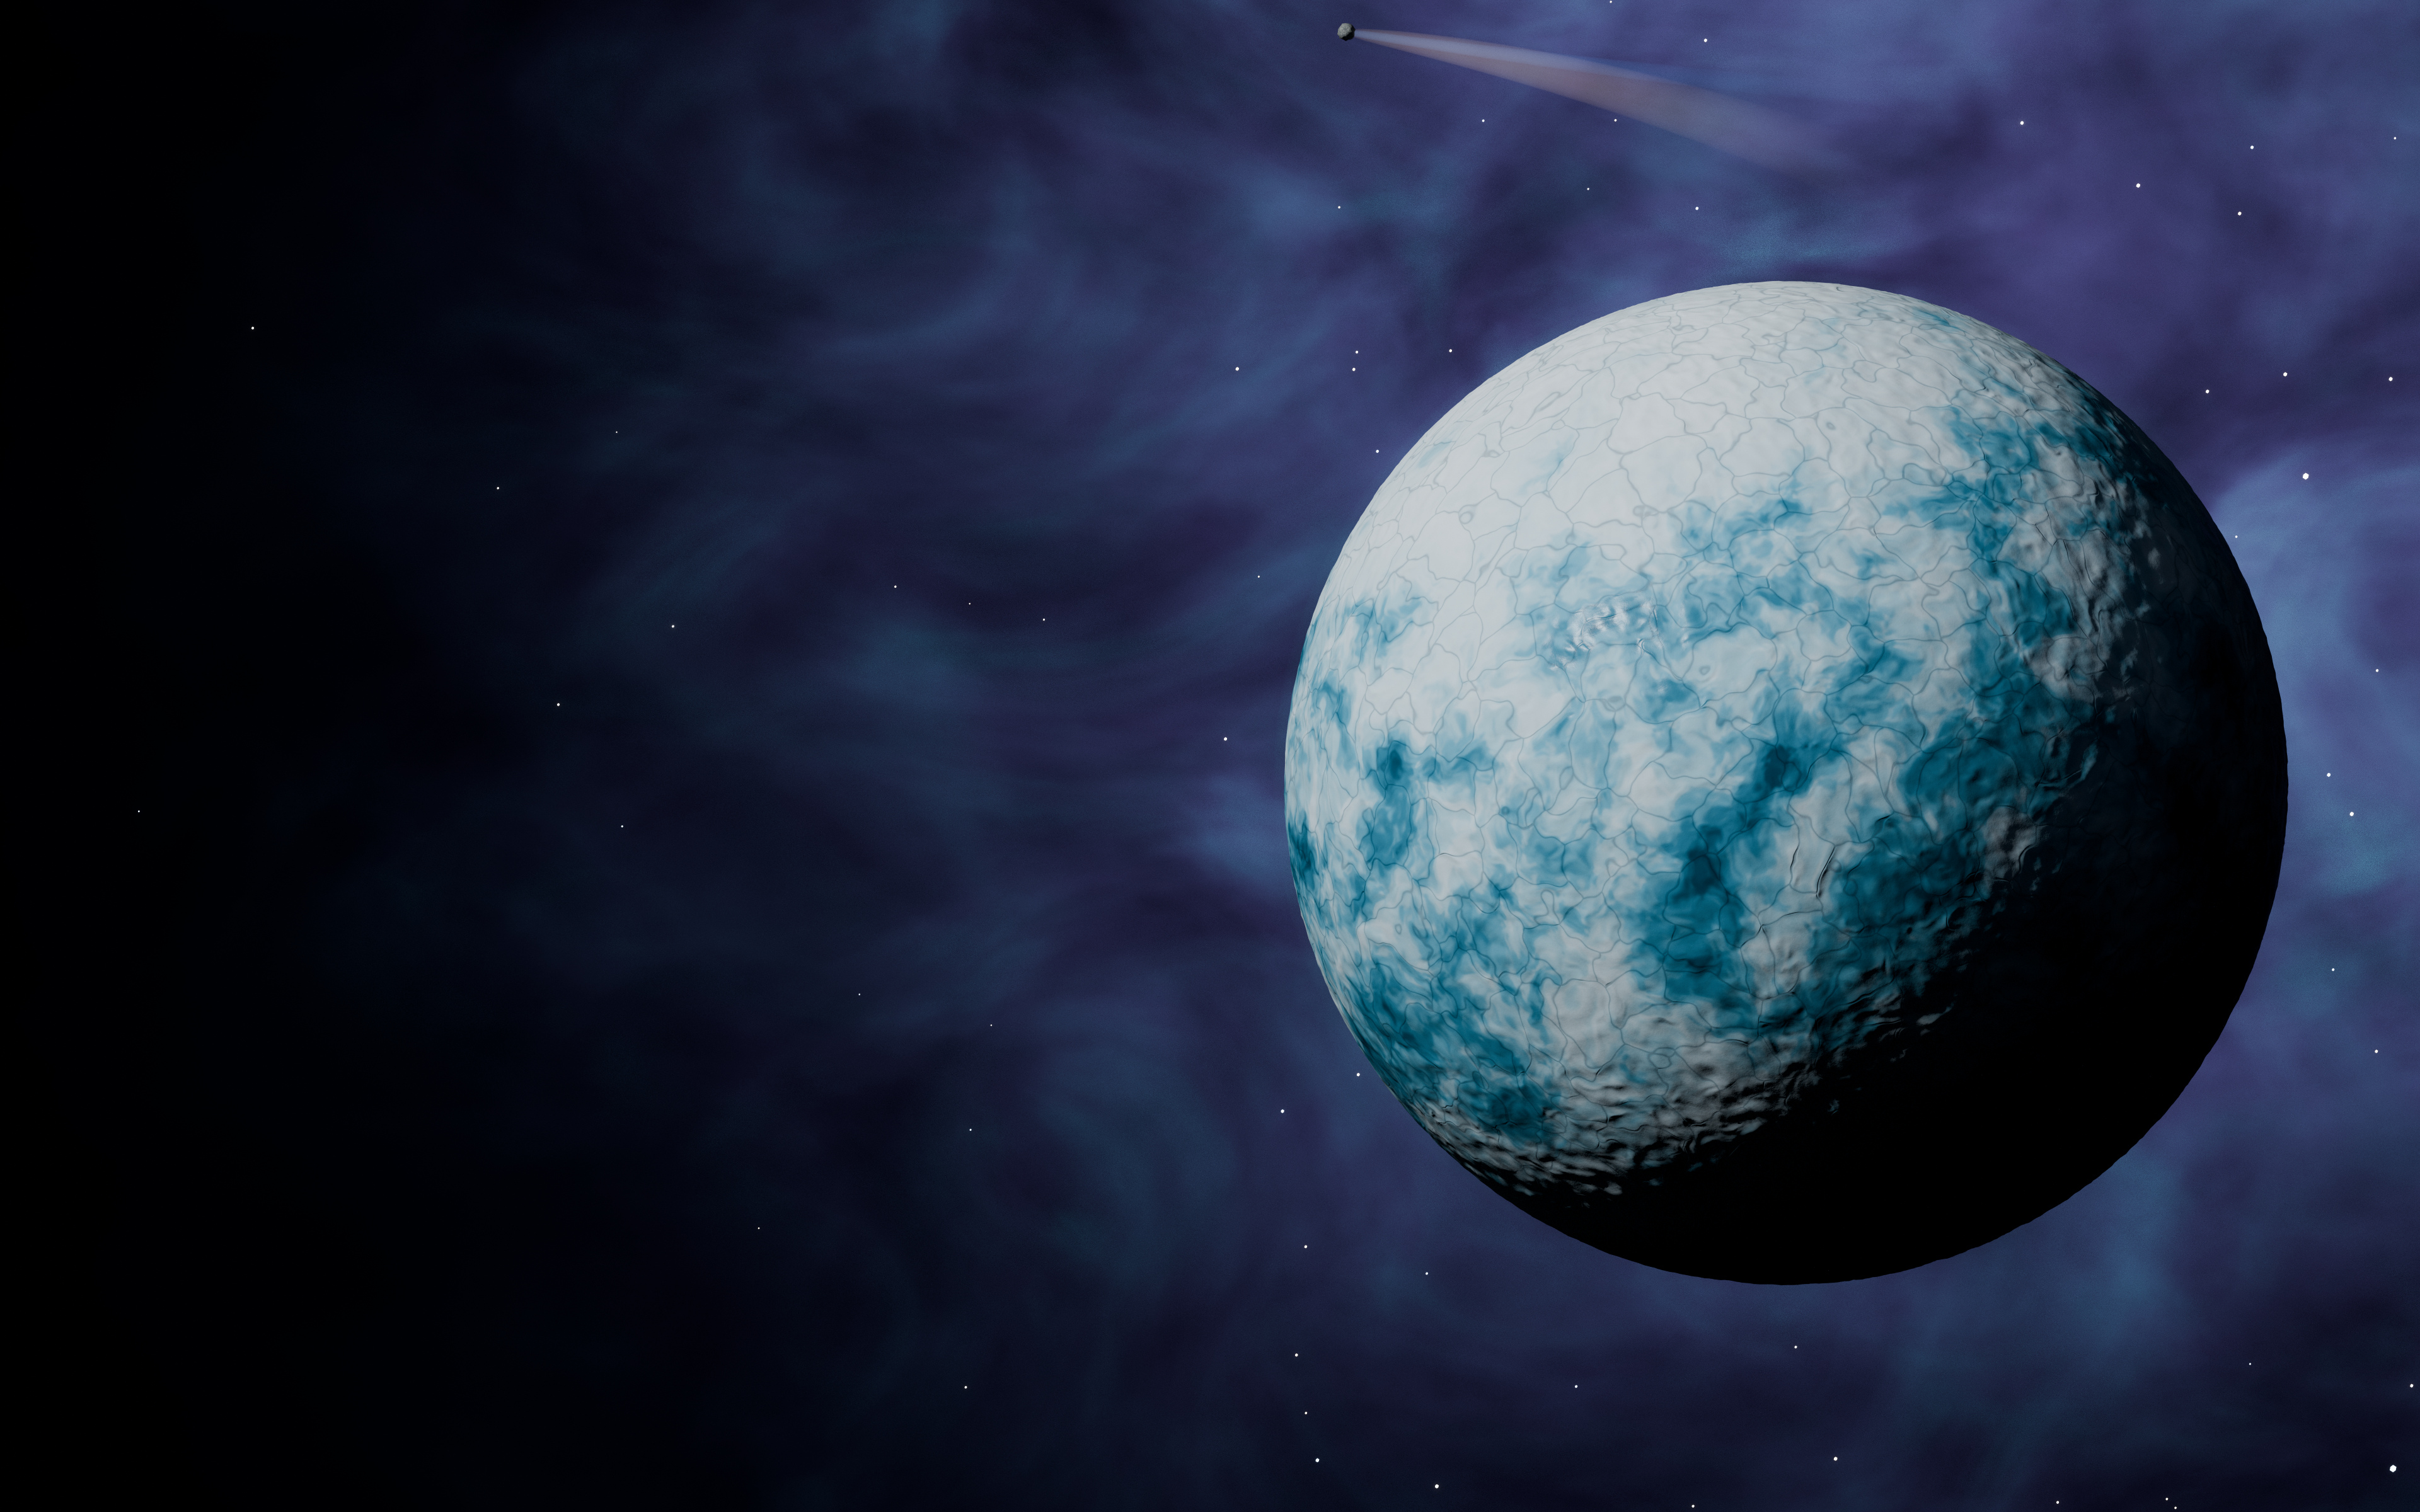
\includegraphics[width=20cm,height=12.5cm]{Risorse/Copertine/M09_Borealis.jpg}};}{}
\node[anchor=north west,inner sep=0] at([xshift=1.05cm,yshift=-1.10cm]current page.north west){\color{Mint}\bfseries\fontsize{23}{28}\selectfont BOREALIS};
\node[anchor=north west,inner sep=0] at([xshift=1.07cm,yshift=-2.16cm]current page.north west){\color{white}\fontsize{9}{12}\selectfont MODULO M09 · SCIENZE DELLA TERRA};
\draw[Mint,line width=1.5pt]([xshift=1.07cm,yshift=-2.78cm]current page.north west)--([xshift=2.6cm,yshift=-2.78cm]current page.north west);
\node[anchor=north west,inner sep=0] at([xshift=1.05cm,yshift=-3.35cm]current page.north west){\begin{minipage}{9.2cm}\raggedright\color{white}\bfseries\fontsize{30}{36}\selectfont Serie\\temporali\\ambientali\end{minipage}};
\node[anchor=north west,inner sep=0] at([xshift=1.07cm,yshift=-7.88cm]current page.north west){\begin{minipage}{8.9cm}\raggedright\color{Lilac}\fontsize{12.2}{17}\selectfont Calendario, dipendenza,\\trasformazioni e stazionarietà\end{minipage}};
\node[anchor=north west,inner sep=0] at([xshift=1.07cm,yshift=-10.52cm]current page.north west){\color{white}\fontsize{11.5}{15}\selectfont Marzio De Corato};
\node[anchor=north west,inner sep=0] at([xshift=1.07cm,yshift=-11.17cm]current page.north west){\color{Mint}\fontsize{8.8}{11}\selectfont\href{https://creativecommons.org/licenses/by-nc-sa/4.0/}{© 2026 · CC BY-NC-SA 4.0}};
\end{tikzpicture}\end{frame}
\begin{frame}[plain]\hypertarget{slide2}{}
\bookmark[level=0,page=2]{Tempo e calendario}
\bookmark[level=1,page=2]{Che cosa perdiamo senza l’ordine temporale?}
\begin{lrbox}{\PilotLeftBox}%
\begin{minipage}[t]{10.05cm}\raggedright\color{Ink}\fontsize{11.3}{14.8}\selectfont
\PLabel{Una stessa distribuzione, due successioni}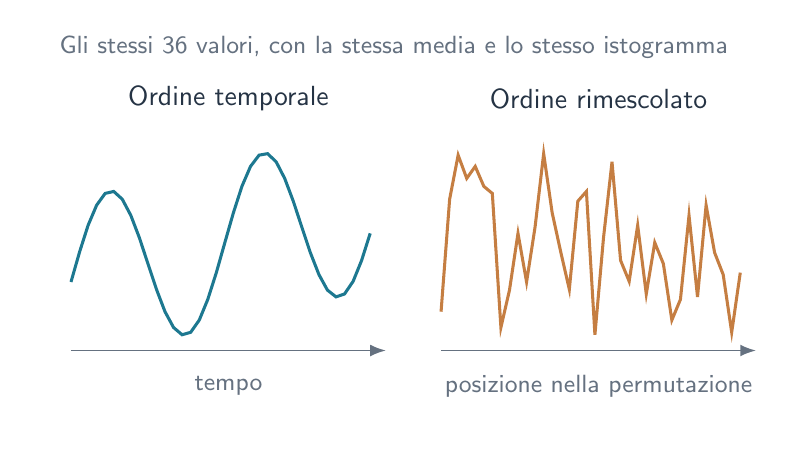
\begin{tikzpicture}[x=1cm,y=1cm]
\path[use as bounding box](-.15,-.15) rectangle(9.4,4.9);
\node[pLabel] at(2.4,4.0){Ordine temporale};\draw[pAxis](0.4,.8)--(4.4,.8);\draw[GeoA,line width=1.1pt] plot coordinates {(0.400,1.670) (0.509,2.051) (0.617,2.389) (0.726,2.646) (0.834,2.795) (0.943,2.820) (1.051,2.722) (1.160,2.516) (1.269,2.231) (1.377,1.903) (1.486,1.576) (1.594,1.293) (1.703,1.092) (1.811,1.000) (1.920,1.031) (2.029,1.186) (2.137,1.448) (2.246,1.789) (2.354,2.170) (2.463,2.550) (2.571,2.885) (2.680,3.138) (2.789,3.281) (2.897,3.300) (3.006,3.196) (3.114,2.986) (3.223,2.697) (3.331,2.369) (3.440,2.043) (3.549,1.764) (3.657,1.567) (3.766,1.481) (3.874,1.518) (3.983,1.678) (4.091,1.944) (4.200,2.288)};\node[pNote] at(2.4,.35){tempo};\node[pLabel] at(7.1000000000000005,4.0){Ordine rimescolato};\draw[pAxis](5.1000000000000005,.8)--(9.100000000000001,.8);\draw[GeoB,line width=1.1pt] plot coordinates {(5.100,1.293) (5.209,2.722) (5.317,3.281) (5.426,2.986) (5.534,3.138) (5.643,2.885) (5.751,2.795) (5.860,1.092) (5.969,1.567) (6.077,2.288) (6.186,1.670) (6.294,2.369) (6.403,3.300) (6.511,2.550) (6.620,2.051) (6.729,1.576) (6.837,2.697) (6.946,2.820) (7.054,1.000) (7.163,2.231) (7.271,3.196) (7.380,1.944) (7.489,1.678) (7.597,2.389) (7.706,1.518) (7.814,2.170) (7.923,1.903) (8.031,1.186) (8.140,1.448) (8.249,2.516) (8.357,1.481) (8.466,2.646) (8.574,2.043) (8.683,1.764) (8.791,1.031) (8.900,1.789)};\node[pNote] at(7.1000000000000005,.35){posizione nella permutazione};\node[pNote] at(4.5,4.65){Gli stessi 36 valori, con la stessa media e lo stesso istogramma};
\end{tikzpicture}
\end{minipage}%
\end{lrbox}
\typeout{FULLBOX:002:L:\the\ht\PilotLeftBox:\the\dp\PilotLeftBox}
\begin{lrbox}{\PilotRightBox}%
\begin{minipage}[t]{7.55cm}\raggedright\color{Ink}\fontsize{11.3}{14.8}\selectfont
\PBody{Rimescolare i valori lascia invariati media, quantili e istogramma. Cambia la relazione fra un’osservazione e quelle che la precedono.}
\vspace{4mm}
\[\mathcal D=\{(t_i,x_i)\}_{i=1}^{n}.\]
\PInfo{La domanda della lezione: quali caratteristiche della serie dipendono dal calendario e dalla successione dei valori?}
\vspace{3mm}
\PBody{Seguiremo una serie storica di CO$_2$ e due archivi simulati, in cui alcune proprietà sono note.}
\end{minipage}%
\end{lrbox}
\typeout{FULLBOX:002:R:\the\ht\PilotRightBox:\the\dp\PilotRightBox}
\begin{tikzpicture}[remember picture,overlay]
\PilotChrome{Che cosa perdiamo senza l’ordine temporale?}{I · TEMPO E CALENDARIO}{2}{Il tempo è una coordinata del dato. La distribuzione dei valori, da sola, non descrive una serie.}
\node[anchor=north west,inner sep=0] at([xshift=0.96cm,yshift=-2.13cm]current page.north west){\usebox{\PilotLeftBox}};
\node[anchor=north west,inner sep=0] at([xshift=11.52cm,yshift=-2.13cm]current page.north west){\usebox{\PilotRightBox}};
\end{tikzpicture}\end{frame}

\begin{frame}[plain]\hypertarget{slide3}{}
\bookmark[level=1,page=3]{Ogni valore ha un tempo e una durata}
\begin{lrbox}{\PilotLeftBox}%
\begin{minipage}[t]{10.05cm}\raggedright\color{Ink}\fontsize{11.3}{14.8}\selectfont
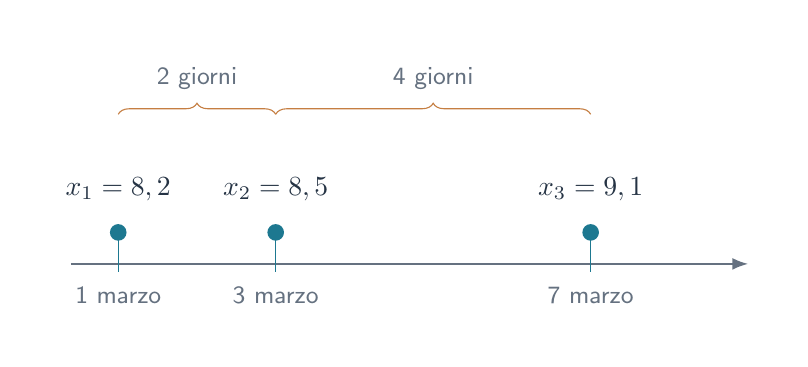
\begin{tikzpicture}[x=1cm,y=1cm]
\path[use as bounding box](-.15,-.15) rectangle(9.4,3.8);
\draw[pAxis](.4,.8)--(9,.8);\draw[GeoA](1,.7)--(1,1.1);\fill[GeoA](1,1.2)circle(3pt);\node[pLabel] at(1,1.75){$x_1=8,2$};\node[pNote] at(1,.4){1 marzo};\draw[GeoA](3,.7)--(3,1.1);\fill[GeoA](3,1.2)circle(3pt);\node[pLabel] at(3,1.75){$x_2=8,5$};\node[pNote] at(3,.4){3 marzo};\draw[GeoA](7,.7)--(7,1.1);\fill[GeoA](7,1.2)circle(3pt);\node[pLabel] at(7,1.75){$x_3=9,1$};\node[pNote] at(7,.4){7 marzo};\draw[decorate,decoration={brace,amplitude=4pt},GeoB](1,2.7)--(3,2.7);\node[pNote] at(2,3.15){2 giorni};\draw[decorate,decoration={brace,amplitude=4pt},GeoB](3,2.7)--(7,2.7);\node[pNote] at(5,3.15){4 giorni};
\end{tikzpicture}\[\Delta t_i=t_i-t_{i-1}.\]
\end{minipage}%
\end{lrbox}
\typeout{FULLBOX:003:L:\the\ht\PilotLeftBox:\the\dp\PilotLeftBox}
\begin{lrbox}{\PilotRightBox}%
\begin{minipage}[t]{7.55cm}\raggedright\color{Ink}\fontsize{11.3}{14.8}\selectfont
\PBody{L’indice $i$ conta le righe. Il tempo $t_i$ indica quando avviene la misura. Passare dalla riga 2 alla riga 3 può significare un giorno, un mese o un intervallo irregolare.}
\vspace{3mm}
\PInfo{Coordinate lungo una carota o una traversa sono spaziali. Si possono studiare dipendenze rispetto alla distanza, dichiarando unità e spaziatura.}
\vspace{3mm}
\PBody{Un ritardo ha significato soltanto quando sappiamo quale intervallo separa le osservazioni.}
\end{minipage}%
\end{lrbox}
\typeout{FULLBOX:003:R:\the\ht\PilotRightBox:\the\dp\PilotRightBox}
\begin{tikzpicture}[remember picture,overlay]
\PilotChrome{Ogni valore ha un tempo e una durata}{I · TEMPO E CALENDARIO}{3}{La distanza fra due tempi osservati deve restare distinguibile dal numero di righe che li separa.}
\node[anchor=north west,inner sep=0] at([xshift=0.96cm,yshift=-2.13cm]current page.north west){\usebox{\PilotLeftBox}};
\node[anchor=north west,inner sep=0] at([xshift=11.52cm,yshift=-2.13cm]current page.north west){\usebox{\PilotRightBox}};
\end{tikzpicture}\end{frame}

\begin{frame}[plain]\hypertarget{slide4}{}
\bookmark[level=1,page=4]{Le date diventano oggetti di R}
\begin{lrbox}{\PilotLeftBox}%
\begin{minipage}[t]{10.05cm}\raggedright\color{Ink}\fontsize{11.3}{14.8}\selectfont
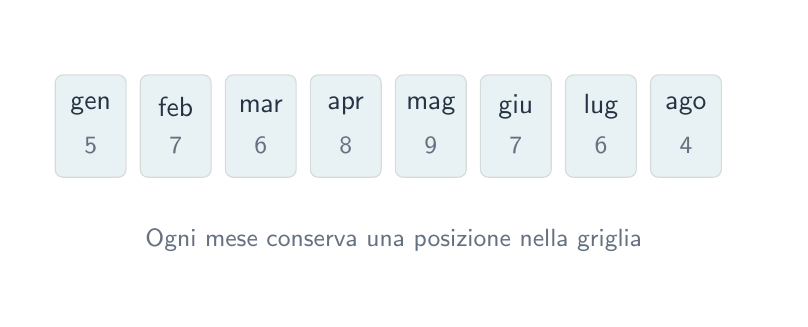
\begin{tikzpicture}[x=1cm,y=1cm]
\path[use as bounding box](-.15,-.15) rectangle(9.4,3.3);
\filldraw[fill=GeoA!10,draw=Rule,rounded corners=1mm](0.2,1.4)rectangle(1.1,2.7);\node[pLabel] at(0.65,2.3){gen};\node[pNote] at(0.65,1.8){5};\filldraw[fill=GeoA!10,draw=Rule,rounded corners=1mm](1.28,1.4)rectangle(2.18,2.7);\node[pLabel] at(1.73,2.3){feb};\node[pNote] at(1.73,1.8){7};\filldraw[fill=GeoA!10,draw=Rule,rounded corners=1mm](2.36,1.4)rectangle(3.2600000000000002,2.7);\node[pLabel] at(2.81,2.3){mar};\node[pNote] at(2.81,1.8){6};\filldraw[fill=GeoA!10,draw=Rule,rounded corners=1mm](3.44,1.4)rectangle(4.34,2.7);\node[pLabel] at(3.89,2.3){apr};\node[pNote] at(3.89,1.8){8};\filldraw[fill=GeoA!10,draw=Rule,rounded corners=1mm](4.5200000000000005,1.4)rectangle(5.420000000000001,2.7);\node[pLabel] at(4.970000000000001,2.3){mag};\node[pNote] at(4.970000000000001,1.8){9};\filldraw[fill=GeoA!10,draw=Rule,rounded corners=1mm](5.6000000000000005,1.4)rectangle(6.500000000000001,2.7);\node[pLabel] at(6.050000000000001,2.3){giu};\node[pNote] at(6.050000000000001,1.8){7};\filldraw[fill=GeoA!10,draw=Rule,rounded corners=1mm](6.680000000000001,1.4)rectangle(7.580000000000001,2.7);\node[pLabel] at(7.130000000000001,2.3){lug};\node[pNote] at(7.130000000000001,1.8){6};\filldraw[fill=GeoA!10,draw=Rule,rounded corners=1mm](7.760000000000001,1.4)rectangle(8.66,2.7);\node[pLabel] at(8.21,2.3){ago};\node[pNote] at(8.21,1.8){4};\node[pNote] at(4.5,.6){Ogni mese conserva una posizione nella griglia};
\end{tikzpicture}\PBody{Una data civile comprende anno, mese e giorno. Il formato anno-mese-giorno evita l’ambiguità fra notazioni italiane e anglosassoni.}
\end{minipage}%
\end{lrbox}
\typeout{FULLBOX:004:L:\the\ht\PilotLeftBox:\the\dp\PilotLeftBox}
\begin{lrbox}{\PilotRightBox}%
\begin{minipage}[t]{7.55cm}\raggedright\color{Ink}\fontsize{11.3}{14.8}\selectfont
\PCode{R · leggere le date}{004_date.R}\PInfo{Una griglia mensile è regolare nel calendario, anche se gli intervalli in giorni hanno durata diversa.}
\end{minipage}%
\end{lrbox}
\typeout{FULLBOX:004:R:\the\ht\PilotRightBox:\the\dp\PilotRightBox}
\begin{tikzpicture}[remember picture,overlay]
\PilotChrome{Le date diventano oggetti di R}{I · TEMPO E CALENDARIO}{4}{La classe Date conserva il calendario. Una successione di mesi non è una successione di 30 giorni.}
\node[anchor=north west,inner sep=0] at([xshift=0.96cm,yshift=-2.13cm]current page.north west){\usebox{\PilotLeftBox}};
\node[anchor=north west,inner sep=0] at([xshift=11.52cm,yshift=-2.13cm]current page.north west){\usebox{\PilotRightBox}};
\end{tikzpicture}\end{frame}

\begin{frame}[plain]\hypertarget{slide5}{}
\bookmark[level=1,page=5]{Istanti e intervalli descrivono misure diverse}
\begin{lrbox}{\PilotLeftBox}%
\begin{minipage}[t]{10.05cm}\raggedright\color{Ink}\fontsize{11.3}{14.8}\selectfont
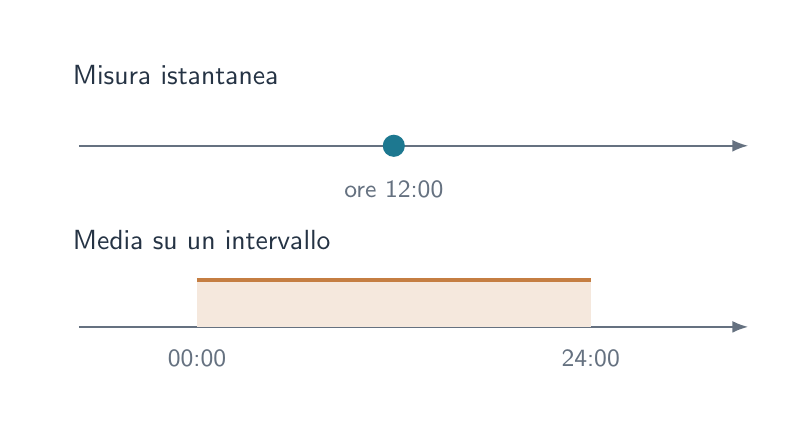
\begin{tikzpicture}[x=1cm,y=1cm]
\path[use as bounding box](-.15,-.15) rectangle(9.4,4.6);
\node[pLabel,anchor=west] at(.3,4){Misura istantanea};\draw[pAxis](.5,3.1)--(9,3.1);\fill[GeoA](4.5,3.1)circle(4pt);\node[pNote] at(4.5,2.55){ore 12:00};\node[pLabel,anchor=west] at(.3,1.9){Media su un intervallo};\draw[pAxis](.5,.8)--(9,.8);\fill[GeoB!18](2,.8)rectangle(7,1.4);\draw[GeoB,line width=1.5pt](2,1.4)--(7,1.4);\node[pNote] at(2,.4){00:00};\node[pNote] at(7,.4){24:00};
\end{tikzpicture}
\end{minipage}%
\end{lrbox}
\typeout{FULLBOX:005:L:\the\ht\PilotLeftBox:\the\dp\PilotLeftBox}
\begin{lrbox}{\PilotRightBox}%
\begin{minipage}[t]{7.55cm}\raggedright\color{Ink}\fontsize{11.3}{14.8}\selectfont
\PBody{Una temperatura alle ore 12 e una media giornaliera riassumono quantità diverse. Alla data occorre associare il significato della misura.}
\vspace{3mm}
\[\bar x_{[a,b]}=\frac{1}{b-a}\int_a^b x(t)\,dt.\]
\PSmall{La formula definisce una media temporale continua ideale. I dati discreti richiedono una regola di approssimazione.}
\vspace{3mm}
\PInfo{Per serie orarie servono anche fuso, ora legale e convenzione dell’istante: inizio, centro o fine dell’intervallo.}
\end{minipage}%
\end{lrbox}
\typeout{FULLBOX:005:R:\the\ht\PilotRightBox:\the\dp\PilotRightBox}
\begin{tikzpicture}[remember picture,overlay]
\PilotChrome{Istanti e intervalli descrivono misure diverse}{I · TEMPO E CALENDARIO}{5}{Data, durata e procedura di misura stabiliscono quale quantità stiamo confrontando.}
\node[anchor=north west,inner sep=0] at([xshift=0.96cm,yshift=-2.13cm]current page.north west){\usebox{\PilotLeftBox}};
\node[anchor=north west,inner sep=0] at([xshift=11.52cm,yshift=-2.13cm]current page.north west){\usebox{\PilotRightBox}};
\end{tikzpicture}\end{frame}

\begin{frame}[plain]\hypertarget{slide6}{}
\bookmark[level=1,page=6]{La provenienza della \texorpdfstring{CO$_2$}{CO2} storica}
\begin{lrbox}{\PilotLeftBox}%
\begin{minipage}[t]{10.05cm}\raggedright\color{Ink}\fontsize{11.3}{14.8}\selectfont
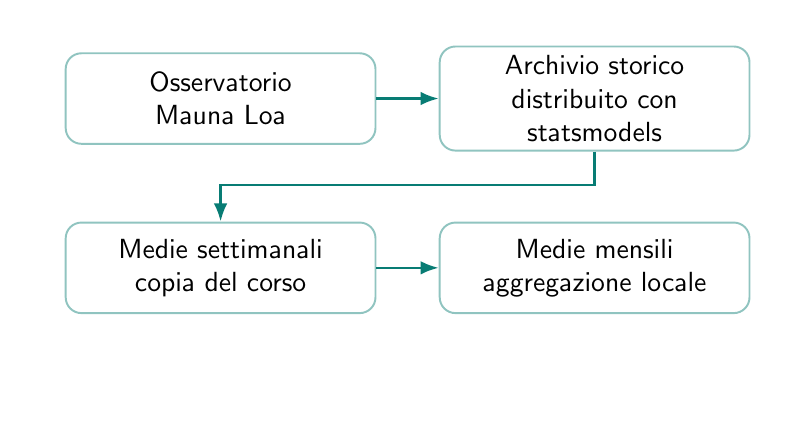
\begin{tikzpicture}[x=1cm,y=1cm]
\path[use as bounding box](-.15,-.15) rectangle(9.4,4.5);
\node[pFlow,text width=3.7cm,minimum height=1.15cm] (p0) at(2.3,3.6){Osservatorio\\Mauna Loa};\node[pFlow,text width=3.7cm,minimum height=1.15cm] (p1) at(7.05,3.6){Archivio storico\\distribuito con statsmodels};\node[pFlow,text width=3.7cm,minimum height=1.15cm] (p2) at(2.3,1.45){Medie settimanali\\copia del corso};\node[pFlow,text width=3.7cm,minimum height=1.15cm] (p3) at(7.05,1.45){Medie mensili\\aggregazione locale};\draw[pEdge](p0.east)--(p1.west);\draw[pEdge](p1.south)--(7.05,2.5)--(2.3,2.5)--(p2.north);\draw[pEdge](p2.east)--(p3.west);
\end{tikzpicture}\PSmall{Fonte: archivio distribuito con statsmodels, attribuito a Keeling e Whorf e al CDIAC.}
\end{minipage}%
\end{lrbox}
\typeout{FULLBOX:006:L:\the\ht\PilotLeftBox:\the\dp\PilotLeftBox}
\begin{lrbox}{\PilotRightBox}%
\begin{minipage}[t]{7.55cm}\raggedright\color{Ink}\fontsize{11.3}{14.8}\selectfont
\PBody{Il file settimanale del corso contiene le concentrazioni storiche dell’osservatorio di Mauna Loa. Il periodo va da marzo 1958 a dicembre 2001.}
\vspace{3mm}
\PInfo{La versione mensile del corso media i valori settimanali disponibili, assegnandoli al mese della data. È un’aggregazione locale documentata.}
\vspace{3mm}
\PBody{Questi dati servono a studiare tendenza, stagione e dipendenza temporale. La data finale dell’archivio resta esplicita in ogni analisi.}
\vspace{2mm}
\PSmall{\href{https://www.statsmodels.org/stable/datasets/generated/co2.html}{Fonte e descrizione dell’archivio storico}}
\end{minipage}%
\end{lrbox}
\typeout{FULLBOX:006:R:\the\ht\PilotRightBox:\the\dp\PilotRightBox}
\begin{tikzpicture}[remember picture,overlay]
\PilotChrome{La provenienza della \texorpdfstring{CO$_2$}{CO2} storica}{I · TEMPO E CALENDARIO}{6}{La media mensile derivata ha una definizione propria. Non va confusa con una serie mensile ufficiale aggiornata.}
\node[anchor=north west,inner sep=0] at([xshift=0.96cm,yshift=-2.13cm]current page.north west){\usebox{\PilotLeftBox}};
\node[anchor=north west,inner sep=0] at([xshift=11.52cm,yshift=-2.13cm]current page.north west){\usebox{\PilotRightBox}};
\end{tikzpicture}\end{frame}

\begin{frame}[plain]\hypertarget{slide7}{}
\bookmark[level=1,page=7]{Una crescita attraversata da oscillazioni}
\begin{lrbox}{\PilotLeftBox}%
\begin{minipage}[t]{10.05cm}\raggedright\color{Ink}\fontsize{11.3}{14.8}\selectfont
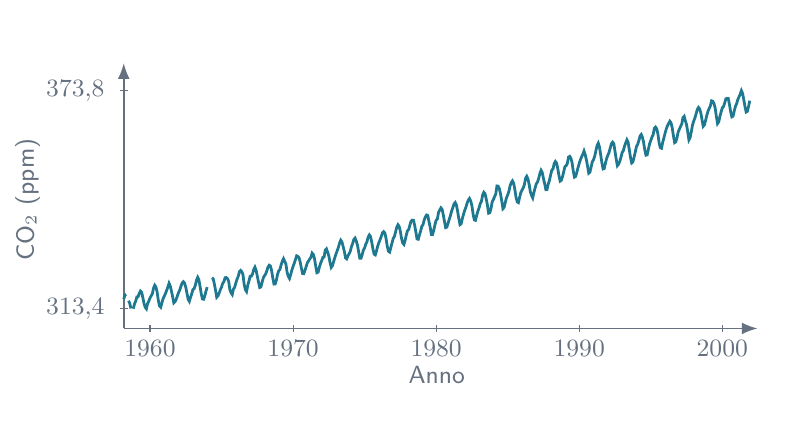
\begin{tikzpicture}[x=1cm,y=1cm]
\path[use as bounding box](-.3,-.2) rectangle(9.299999999999999,4.5);
\draw[pAxis](0.92,0.68)--(8.969999999999999,0.68);
\draw[pAxis](0.92,0.68)--(0.92,4.050000000000001);
\draw[Muted](1.2531,0.63)--(1.2531,0.7300000000000001);\node[pNote] at(1.2531,0.43000000000000005){$1960$};
\draw[Muted](3.0703,0.63)--(3.0703,0.7300000000000001);\node[pNote] at(3.0703,0.43000000000000005){$1970$};
\draw[Muted](4.8874,0.63)--(4.8874,0.7300000000000001);\node[pNote] at(4.8874,0.43000000000000005){$1980$};
\draw[Muted](6.7046,0.63)--(6.7046,0.7300000000000001);\node[pNote] at(6.7046,0.43000000000000005){$1990$};
\draw[Muted](8.5217,0.63)--(8.5217,0.7300000000000001);\node[pNote] at(8.5217,0.43000000000000005){$2000$};
\draw[Muted](0.87,0.9294)--(0.9700000000000001,0.9294);\node[pNote,anchor=east] at(0.8,0.9294){$313{,}4$};
\draw[Muted](0.87,3.7006)--(0.9700000000000001,3.7006);\node[pNote,anchor=east] at(0.8,3.7006){$373{,}8$};
\node[pNote] at(4.895,0.09000000000000008){Anno};
\node[pNote,rotate=90] at(-.3,2.3150000000000004){CO$_2$ (ppm)};
\draw[GeoA,line width=1.0pt] plot coordinates {(0.9200,1.0533) (0.9351,1.1038) (0.9503,1.1145)};
\draw[GeoA,line width=1.0pt] plot coordinates {(0.9806,1.0315) (0.9957,1.0005) (1.0109,0.9340)};
\draw[GeoA,line width=1.0pt] plot coordinates {(1.0411,0.9306) (1.0563,0.9891) (1.0714,1.0258) (1.0866,1.0808) (1.1017,1.0823) (1.1169,1.1255) (1.1320,1.1554) (1.1471,1.1416) (1.1623,1.0728) (1.1774,0.9982) (1.1926,0.9489) (1.2077,0.9294) (1.2229,0.9971) (1.2380,1.0269) (1.2531,1.0661) (1.2683,1.0934) (1.2834,1.1210) (1.2986,1.1918) (1.3137,1.2288) (1.3289,1.2070) (1.3440,1.1432) (1.3591,1.0384) (1.3743,0.9650) (1.3894,0.9496) (1.4046,1.0040) (1.4197,1.0579) (1.4349,1.0911) (1.4500,1.1244) (1.4651,1.1645) (1.4803,1.2056) (1.4954,1.2540) (1.5106,1.2207) (1.5257,1.1551) (1.5409,1.0843) (1.5560,1.0047) (1.5711,1.0189) (1.5863,1.0510) (1.6014,1.0937) (1.6166,1.1370) (1.6317,1.1691) (1.6469,1.2175) (1.6620,1.2575) (1.6771,1.2735) (1.6923,1.2552) (1.7074,1.2058) (1.7226,1.1282) (1.7377,1.0518) (1.7529,1.0246) (1.7680,1.0739) (1.7831,1.1187) (1.7983,1.1737) (1.8134,1.1848) (1.8286,1.2258) (1.8437,1.2907) (1.8589,1.3286) (1.8740,1.2992) (1.8891,1.2139) (1.9043,1.1221) (1.9194,1.0556) (1.9346,1.0510) (1.9497,1.0946) (1.9649,1.1565) (1.9800,1.2047)};
\draw[GeoA,line width=1.0pt] plot coordinates {(2.0406,1.3240) (2.0557,1.3125) (2.0709,1.2460) (2.0860,1.1634) (2.1011,1.0762) (2.1163,1.0927) (2.1314,1.1278) (2.1466,1.1714) (2.1617,1.2047) (2.1769,1.2529) (2.1920,1.2747) (2.2071,1.3240) (2.2223,1.3267) (2.2374,1.3137) (2.2526,1.2799) (2.2677,1.1737) (2.2829,1.1324) (2.2980,1.1102) (2.3131,1.1806) (2.3283,1.2012) (2.3434,1.2570) (2.3586,1.3045) (2.3737,1.3412) (2.3889,1.4001) (2.4040,1.4169) (2.4191,1.4020) (2.4343,1.3630) (2.4494,1.2414) (2.4646,1.1726) (2.4797,1.1487) (2.4949,1.2276) (2.5100,1.2809) (2.5251,1.3423) (2.5403,1.3435) (2.5554,1.3699) (2.5706,1.4286) (2.5857,1.4593) (2.6009,1.4192) (2.6160,1.3460) (2.6311,1.2712) (2.6463,1.2001) (2.6614,1.2070) (2.6766,1.2632) (2.6917,1.3203) (2.7069,1.3492) (2.7220,1.3722) (2.7371,1.4121) (2.7523,1.4605) (2.7674,1.4834) (2.7826,1.4736) (2.7977,1.4169) (2.8129,1.3212) (2.8280,1.2437) (2.8431,1.2448) (2.8583,1.2928) (2.8734,1.3664) (2.8886,1.4123) (2.9037,1.4284) (2.9189,1.4891) (2.9340,1.5339) (2.9491,1.5662) (2.9643,1.5327) (2.9794,1.4983) (2.9946,1.3946) (3.0097,1.3423) (3.0249,1.3148) (3.0400,1.3616) (3.0551,1.4215) (3.0703,1.4653) (3.0854,1.5086) (3.1006,1.5534) (3.1157,1.6027) (3.1309,1.5956) (3.1460,1.5786) (3.1611,1.5213) (3.1763,1.4460) (3.1914,1.3767) (3.2066,1.3763) (3.2217,1.4180) (3.2369,1.4662) (3.2520,1.5139) (3.2671,1.5373) (3.2823,1.5626) (3.2974,1.5844) (3.3126,1.6369) (3.3277,1.6211) (3.3429,1.5635) (3.3580,1.4731) (3.3731,1.3882) (3.3883,1.3946) (3.4034,1.4536) (3.4186,1.5041) (3.4337,1.5405) (3.4489,1.5821) (3.4640,1.5866) (3.4791,1.6745) (3.4943,1.6910) (3.5094,1.6486) (3.5246,1.6011) (3.5397,1.5190) (3.5549,1.4552) (3.5700,1.4754) (3.5851,1.5270) (3.6003,1.5782) (3.6154,1.6245) (3.6306,1.6669) (3.6457,1.7085) (3.6609,1.7633) (3.6760,1.8011) (3.6911,1.7800) (3.7063,1.7208) (3.7214,1.6601) (3.7366,1.5763) (3.7517,1.5637) (3.7669,1.6016) (3.7820,1.6286) (3.7971,1.6601) (3.8123,1.7197) (3.8274,1.7598) (3.8426,1.8115) (3.8577,1.8275) (3.8729,1.7901) (3.8880,1.7403) (3.9031,1.6552) (3.9183,1.5706) (3.9334,1.5706) (3.9486,1.6176) (3.9637,1.6761) (3.9789,1.7025) (3.9940,1.7507) (4.0091,1.7828) (4.0243,1.8413) (4.0394,1.8681) (4.0546,1.8470) (4.0697,1.7736) (4.0849,1.6901) (4.1000,1.6234) (4.1151,1.6142) (4.1303,1.6653) (4.1454,1.7266) (4.1606,1.7709) (4.1757,1.8080) (4.1909,1.8493) (4.2060,1.8952) (4.2211,1.9094) (4.2363,1.8929) (4.2514,1.8222) (4.2666,1.7243) (4.2817,1.6612) (4.2969,1.6497) (4.3120,1.7071) (4.3271,1.7656) (4.3423,1.8232) (4.3574,1.8482) (4.3726,1.9067) (4.3877,1.9681) (4.4029,1.9973) (4.4180,1.9755) (4.4331,1.9113) (4.4483,1.8229) (4.4634,1.7633) (4.4786,1.7461) (4.4937,1.7988) (4.5089,1.8681) (4.5240,1.9216) (4.5391,1.9365) (4.5543,1.9938) (4.5694,2.0416) (4.5846,2.0558) (4.5997,2.0546) (4.6149,1.9892) (4.6300,1.9044) (4.6451,1.8167) (4.6603,1.8126) (4.6754,1.8665) (4.6906,1.9186) (4.7057,1.9766) (4.7209,1.9984) (4.7360,2.0581) (4.7511,2.0982) (4.7663,2.1212) (4.7814,2.1150) (4.7966,2.0363) (4.8117,1.9675) (4.8269,1.8736) (4.8420,1.8723) (4.8571,1.9273) (4.8723,1.9966) (4.8874,2.0546) (4.9026,2.0684) (4.9177,2.1526) (4.9329,2.1842) (4.9480,2.2113) (4.9631,2.1934) (4.9783,2.1212) (4.9934,2.0397) (5.0086,1.9606) (5.0237,1.9675) (5.0389,2.0149) (5.0540,2.0672) (5.0691,2.1140) (5.0843,2.1705) (5.0994,2.2141) (5.1146,2.2622) (5.1297,2.2792) (5.1449,2.2473) (5.1600,2.1693) (5.1751,2.0764) (5.1903,1.9984) (5.2054,2.0094) (5.2206,2.0776) (5.2357,2.1315) (5.2509,2.1819) (5.2660,2.2209) (5.2811,2.2726) (5.2963,2.3093) (5.3114,2.3315) (5.3266,2.3012) (5.3417,2.2379) (5.3569,2.1326) (5.3720,2.0592) (5.3871,2.0535) (5.4023,2.1166) (5.4174,2.1693) (5.4326,2.2113) (5.4477,2.2645) (5.4629,2.2944) (5.4780,2.3746) (5.4931,2.4091) (5.5083,2.3918) (5.5234,2.3251) (5.5386,2.2485) (5.5537,2.1441) (5.5689,2.1507) (5.5840,2.2026) (5.5991,2.2866) (5.6143,2.3184) (5.6294,2.3529) (5.6446,2.3873) (5.6597,2.4893) (5.6749,2.4871) (5.6900,2.4554) (5.7051,2.3884) (5.7203,2.3012) (5.7354,2.2012) (5.7506,2.2175) (5.7657,2.2806) (5.7809,2.3398) (5.7960,2.3758) (5.8111,2.4194) (5.8263,2.4912) (5.8414,2.5318) (5.8566,2.5547) (5.8717,2.5251) (5.8869,2.4458) (5.9020,2.3471) (5.9171,2.2875) (5.9323,2.2783) (5.9474,2.3434) (5.9626,2.4056) (5.9777,2.4366) (5.9929,2.4630) (6.0080,2.5049) (6.0231,2.5868) (6.0383,2.6123) (6.0534,2.5800) (6.0686,2.5088) (6.0837,2.4169) (6.0989,2.3701) (6.1140,2.3379) (6.1291,2.4077) (6.1443,2.4653) (6.1594,2.5169) (6.1746,2.5398) (6.1897,2.5845) (6.2049,2.6476) (6.2200,2.6885) (6.2351,2.6614) (6.2503,2.5834) (6.2654,2.5205) (6.2806,2.4435) (6.2957,2.4453) (6.3109,2.5134) (6.3260,2.5593) (6.3411,2.6270) (6.3563,2.6901) (6.3714,2.7061) (6.3866,2.7729) (6.4017,2.8002) (6.4169,2.7807) (6.4320,2.7105) (6.4471,2.6224) (6.4623,2.5513) (6.4774,2.5609) (6.4926,2.6086) (6.5077,2.6710) (6.5229,2.7360) (6.5380,2.7463) (6.5531,2.7738) (6.5683,2.8546) (6.5834,2.8656) (6.5986,2.8438) (6.6137,2.7857) (6.6289,2.6809) (6.6440,2.6022) (6.6591,2.6109) (6.6743,2.6637) (6.6894,2.7224) (6.7046,2.7761) (6.7197,2.8220) (6.7349,2.8601) (6.7500,2.8919) (6.7651,2.9332) (6.7803,2.8876) (6.7954,2.8231) (6.8106,2.7417) (6.8257,2.6518) (6.8409,2.6648) (6.8560,2.7325) (6.8711,2.7986) (6.8863,2.8231) (6.9014,2.8679) (6.9166,2.9390) (6.9317,3.0032) (6.9469,3.0330) (6.9620,2.9839) (6.9771,2.8862) (6.9923,2.7857) (7.0074,2.7061) (7.0226,2.7119) (7.0377,2.7802) (7.0529,2.8392) (7.0680,2.8793) (7.0831,2.9151) (7.0983,2.9711) (7.1134,3.0250) (7.1286,3.0463) (7.1437,3.0273) (7.1589,2.9298) (7.1740,2.8316) (7.1891,2.7474) (7.2043,2.7655) (7.2194,2.8013) (7.2346,2.8541) (7.2497,2.9151) (7.2649,2.9378) (7.2800,2.9952) (7.2951,3.0365) (7.3103,3.0757) (7.3254,3.0445) (7.3406,2.9491) (7.3557,2.8529) (7.3709,2.7818) (7.3860,2.7949) (7.4011,2.8541) (7.4163,2.9195) (7.4314,2.9904) (7.4466,3.0170) (7.4617,3.0640) (7.4769,3.1234) (7.4920,3.1431) (7.5071,3.1087) (7.5223,3.0427) (7.5374,2.9470) (7.5526,2.8805) (7.5677,2.8848) (7.5829,2.9562) (7.5980,3.0243) (7.6131,3.0663) (7.6283,3.1099) (7.6434,3.1397) (7.6586,3.2216) (7.6737,3.2372) (7.6889,3.2166) (7.7040,3.1500) (7.7191,3.0388) (7.7343,2.9757) (7.7494,2.9688) (7.7646,3.0434) (7.7797,3.0996) (7.7949,3.1603) (7.8100,3.2131) (7.8251,3.2537) (7.8403,3.2831) (7.8554,3.3118) (7.8706,3.2913) (7.8857,3.2269) (7.9009,3.1280) (7.9160,3.0399) (7.9311,3.0502) (7.9463,3.1014) (7.9614,3.1764) (7.9766,3.2108) (7.9917,3.2452) (8.0069,3.2767) (8.0220,3.3576) (8.0371,3.3739) (8.0523,3.3186) (8.0674,3.2682) (8.0826,3.1803) (8.0977,3.0743) (8.1129,3.1019) (8.1280,3.1766) (8.1431,3.2624) (8.1583,3.3124) (8.1734,3.3519) (8.1886,3.4058) (8.2037,3.4586) (8.2189,3.4868) (8.2340,3.4689) (8.2491,3.4161) (8.2643,3.3299) (8.2794,3.2475) (8.2946,3.2656) (8.3097,3.3221) (8.3249,3.3852) (8.3400,3.4400) (8.3551,3.4735) (8.3703,3.5079) (8.3854,3.5710) (8.4006,3.5648) (8.4157,3.5377) (8.4309,3.4804) (8.4460,3.3748) (8.4611,3.2819) (8.4763,3.3033) (8.4914,3.3725) (8.5066,3.4299) (8.5217,3.4813) (8.5369,3.4976) (8.5520,3.5446) (8.5671,3.5969) (8.5823,3.6019) (8.5974,3.6008) (8.6126,3.5235) (8.6277,3.4322) (8.6429,3.3675) (8.6580,3.3760) (8.6731,3.4402) (8.6883,3.5006) (8.7034,3.5343) (8.7186,3.5870) (8.7337,3.6208) (8.7489,3.6536) (8.7640,3.7006) (8.7791,3.6666) (8.7943,3.5859) (8.8094,3.4999) (8.8246,3.4290) (8.8397,3.4368) (8.8549,3.4976) (8.8700,3.5730)};
\end{tikzpicture}\PSmall{Medie mensili derivate. Gli intervalli privi di valori restano interruzioni della linea.}
\end{minipage}%
\end{lrbox}
\typeout{FULLBOX:007:L:\the\ht\PilotLeftBox:\the\dp\PilotLeftBox}
\begin{lrbox}{\PilotRightBox}%
\begin{minipage}[t]{7.55cm}\raggedright\color{Ink}\fontsize{11.3}{14.8}\selectfont
\PCode{R · contare le osservazioni}{007_archivio.R}\PInfo{La crescita di lungo periodo e le oscillazioni annuali pongono domande diverse. Le esamineremo separatamente.}
\end{minipage}%
\end{lrbox}
\typeout{FULLBOX:007:R:\the\ht\PilotRightBox:\the\dp\PilotRightBox}
\begin{tikzpicture}[remember picture,overlay]
\PilotChrome{Una crescita attraversata da oscillazioni}{I · TEMPO E CALENDARIO}{7}{Un grafico della serie deve mostrare periodo, unità e assenze prima di qualsiasi trasformazione.}
\node[anchor=north west,inner sep=0] at([xshift=0.96cm,yshift=-2.13cm]current page.north west){\usebox{\PilotLeftBox}};
\node[anchor=north west,inner sep=0] at([xshift=11.52cm,yshift=-2.13cm]current page.north west){\usebox{\PilotRightBox}};
\end{tikzpicture}\end{frame}

\begin{frame}[plain]\hypertarget{slide8}{}
\bookmark[level=1,page=8]{La tabella conserva valore e copertura}
\begin{lrbox}{\PilotLeftBox}%
\begin{minipage}[t]{10.05cm}\raggedright\color{Ink}\fontsize{11.3}{14.8}\selectfont
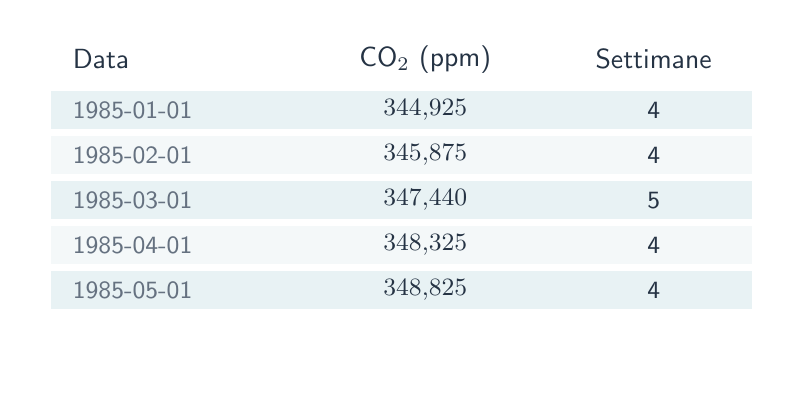
\begin{tikzpicture}[x=1cm,y=1cm]
\path[use as bounding box](-.15,-.15) rectangle(9.4,4.2);
\node[pLabel,anchor=west] at(.3,3.8){Data};\node[pLabel] at(4.9,3.8){CO$_2$ (ppm)};\node[pLabel] at(7.8,3.8){Settimane};\fill[GeoA!10](.15,2.91) rectangle(9.05,3.3899999999999997);\node[pNote,anchor=west] at(.3,3.15){1985-01-01};\node[pNote,text=Ink] at(4.9,3.15){$ 344{,}925 $};\node[pNote,text=Ink] at(7.8,3.15){4};\fill[GeoA!5](.15,2.34) rectangle(9.05,2.8200000000000003);\node[pNote,anchor=west] at(.3,2.58){1985-02-01};\node[pNote,text=Ink] at(4.9,2.58){$ 345{,}875 $};\node[pNote,text=Ink] at(7.8,2.58){4};\fill[GeoA!10](.15,1.7699999999999998) rectangle(9.05,2.25);\node[pNote,anchor=west] at(.3,2.01){1985-03-01};\node[pNote,text=Ink] at(4.9,2.01){$ 347{,}440 $};\node[pNote,text=Ink] at(7.8,2.01){5};\fill[GeoA!5](.15,1.2) rectangle(9.05,1.68);\node[pNote,anchor=west] at(.3,1.44){1985-04-01};\node[pNote,text=Ink] at(4.9,1.44){$ 348{,}325 $};\node[pNote,text=Ink] at(7.8,1.44){4};\fill[GeoA!10](.15,0.6300000000000001) rectangle(9.05,1.11);\node[pNote,anchor=west] at(.3,0.8700000000000001){1985-05-01};\node[pNote,text=Ink] at(4.9,0.8700000000000001){$ 348{,}825 $};\node[pNote,text=Ink] at(7.8,0.8700000000000001){4};
\end{tikzpicture}\PSmall{Prime cinque righe del segmento 1985–2001. La copertura conta i valori settimanali disponibili.}
\end{minipage}%
\end{lrbox}
\typeout{FULLBOX:008:L:\the\ht\PilotLeftBox:\the\dp\PilotLeftBox}
\begin{lrbox}{\PilotRightBox}%
\begin{minipage}[t]{7.55cm}\raggedright\color{Ink}\fontsize{11.3}{14.8}\selectfont
\PCode{R · riconoscere le colonne}{008_tabella.R}\PBody{La concentrazione e il numero di settimane devono viaggiare insieme. Due medie uguali possono poggiare su quantità diverse di osservazioni.}
\end{minipage}%
\end{lrbox}
\typeout{FULLBOX:008:R:\the\ht\PilotRightBox:\the\dp\PilotRightBox}
\begin{tikzpicture}[remember picture,overlay]
\PilotChrome{La tabella conserva valore e copertura}{I · TEMPO E CALENDARIO}{8}{La copertura è un’informazione sulla misura aggregata e deve rimanere nella tabella.}
\node[anchor=north west,inner sep=0] at([xshift=0.96cm,yshift=-2.13cm]current page.north west){\usebox{\PilotLeftBox}};
\node[anchor=north west,inner sep=0] at([xshift=11.52cm,yshift=-2.13cm]current page.north west){\usebox{\PilotRightBox}};
\end{tikzpicture}\end{frame}

\begin{frame}[plain]\hypertarget{slide9}{}
\bookmark[level=1,page=9]{L’ordinamento segue il calendario}
\begin{lrbox}{\PilotLeftBox}%
\begin{minipage}[t]{10.05cm}\raggedright\color{Ink}\fontsize{11.3}{14.8}\selectfont
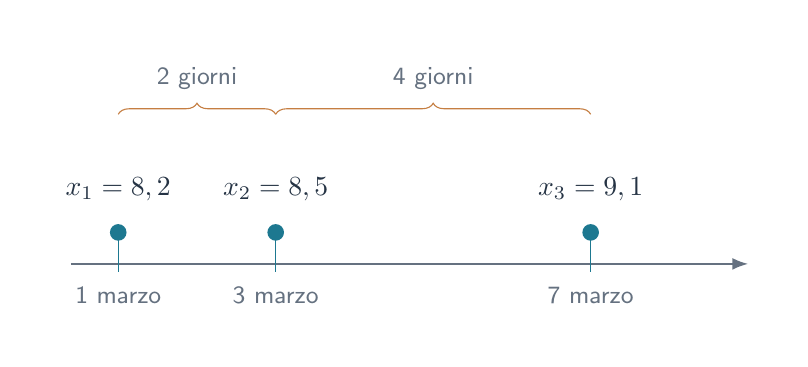
\begin{tikzpicture}[x=1cm,y=1cm]
\path[use as bounding box](-.15,-.15) rectangle(9.4,3.8);
\draw[pAxis](.4,.8)--(9,.8);\draw[GeoA](1,.7)--(1,1.1);\fill[GeoA](1,1.2)circle(3pt);\node[pLabel] at(1,1.75){$x_1=8,2$};\node[pNote] at(1,.4){1 marzo};\draw[GeoA](3,.7)--(3,1.1);\fill[GeoA](3,1.2)circle(3pt);\node[pLabel] at(3,1.75){$x_2=8,5$};\node[pNote] at(3,.4){3 marzo};\draw[GeoA](7,.7)--(7,1.1);\fill[GeoA](7,1.2)circle(3pt);\node[pLabel] at(7,1.75){$x_3=9,1$};\node[pNote] at(7,.4){7 marzo};\draw[decorate,decoration={brace,amplitude=4pt},GeoB](1,2.7)--(3,2.7);\node[pNote] at(2,3.15){2 giorni};\draw[decorate,decoration={brace,amplitude=4pt},GeoB](3,2.7)--(7,2.7);\node[pNote] at(5,3.15){4 giorni};
\end{tikzpicture}\PInfo{Il controllo delle date avviene prima dell’assegnazione di una frequenza alla serie.}
\end{minipage}%
\end{lrbox}
\typeout{FULLBOX:009:L:\the\ht\PilotLeftBox:\the\dp\PilotLeftBox}
\begin{lrbox}{\PilotRightBox}%
\begin{minipage}[t]{7.55cm}\raggedright\color{Ink}\fontsize{11.3}{14.8}\selectfont
\PCode{R · ordinare tutte le colonne}{009_ordinare.R}\PBody{Ordinare soltanto i valori romperebbe l’associazione con date e metadati. Ogni riga deve restare integra.}
\end{minipage}%
\end{lrbox}
\typeout{FULLBOX:009:R:\the\ht\PilotRightBox:\the\dp\PilotRightBox}
\begin{tikzpicture}[remember picture,overlay]
\PilotChrome{L’ordinamento segue il calendario}{I · TEMPO E CALENDARIO}{9}{La serie ordinata conserva le associazioni fra date, valori e informazioni sulla misura.}
\node[anchor=north west,inner sep=0] at([xshift=0.96cm,yshift=-2.13cm]current page.north west){\usebox{\PilotLeftBox}};
\node[anchor=north west,inner sep=0] at([xshift=11.52cm,yshift=-2.13cm]current page.north west){\usebox{\PilotRightBox}};
\end{tikzpicture}\end{frame}

\begin{frame}[plain]\hypertarget{slide10}{}
\bookmark[level=1,page=10]{Un’assenza occupa una posizione}
\begin{lrbox}{\PilotLeftBox}%
\begin{minipage}[t]{10.05cm}\raggedright\color{Ink}\fontsize{11.3}{14.8}\selectfont
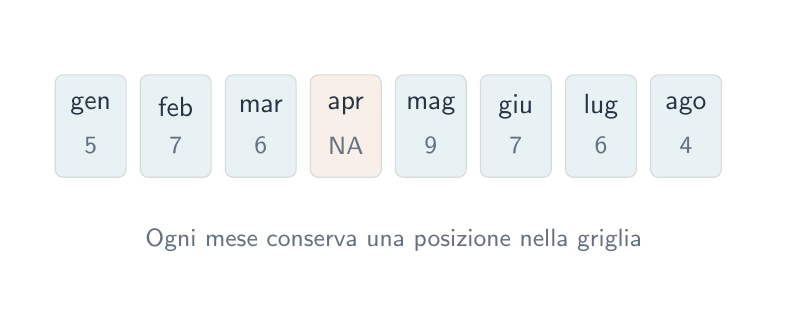
\begin{tikzpicture}[x=1cm,y=1cm]
\path[use as bounding box](-.15,-.15) rectangle(9.4,3.3);
\filldraw[fill=GeoA!10,draw=Rule,rounded corners=1mm](0.2,1.4)rectangle(1.1,2.7);\node[pLabel] at(0.65,2.3){gen};\node[pNote] at(0.65,1.8){5};\filldraw[fill=GeoA!10,draw=Rule,rounded corners=1mm](1.28,1.4)rectangle(2.18,2.7);\node[pLabel] at(1.73,2.3){feb};\node[pNote] at(1.73,1.8){7};\filldraw[fill=GeoA!10,draw=Rule,rounded corners=1mm](2.36,1.4)rectangle(3.2600000000000002,2.7);\node[pLabel] at(2.81,2.3){mar};\node[pNote] at(2.81,1.8){6};\filldraw[fill=GeoB!12,draw=Rule,rounded corners=1mm](3.44,1.4)rectangle(4.34,2.7);\node[pLabel] at(3.89,2.3){apr};\node[pNote] at(3.89,1.8){NA};\filldraw[fill=GeoA!10,draw=Rule,rounded corners=1mm](4.5200000000000005,1.4)rectangle(5.420000000000001,2.7);\node[pLabel] at(4.970000000000001,2.3){mag};\node[pNote] at(4.970000000000001,1.8){9};\filldraw[fill=GeoA!10,draw=Rule,rounded corners=1mm](5.6000000000000005,1.4)rectangle(6.500000000000001,2.7);\node[pLabel] at(6.050000000000001,2.3){giu};\node[pNote] at(6.050000000000001,1.8){7};\filldraw[fill=GeoA!10,draw=Rule,rounded corners=1mm](6.680000000000001,1.4)rectangle(7.580000000000001,2.7);\node[pLabel] at(7.130000000000001,2.3){lug};\node[pNote] at(7.130000000000001,1.8){6};\filldraw[fill=GeoA!10,draw=Rule,rounded corners=1mm](7.760000000000001,1.4)rectangle(8.66,2.7);\node[pLabel] at(8.21,2.3){ago};\node[pNote] at(8.21,1.8){4};\node[pNote] at(4.5,.6){Ogni mese conserva una posizione nella griglia};
\end{tikzpicture}\PBody{Aprile resta nella griglia con valore NA. La distanza fra marzo e maggio continua a essere di due mesi.}
\end{minipage}%
\end{lrbox}
\typeout{FULLBOX:010:L:\the\ht\PilotLeftBox:\the\dp\PilotLeftBox}
\begin{lrbox}{\PilotRightBox}%
\begin{minipage}[t]{7.55cm}\raggedright\color{Ink}\fontsize{11.3}{14.8}\selectfont
\PCode{R · conservare il mese assente}{010_assenze.R}\PInfo{Sostituire NA con zero affermerebbe che il valore osservato è nullo. È un’informazione diversa da un’assenza.}
\end{minipage}%
\end{lrbox}
\typeout{FULLBOX:010:R:\the\ht\PilotRightBox:\the\dp\PilotRightBox}
\begin{tikzpicture}[remember picture,overlay]
\PilotChrome{Un’assenza occupa una posizione}{I · TEMPO E CALENDARIO}{10}{Un valore mancante e un valore nullo esprimono situazioni diverse.}
\node[anchor=north west,inner sep=0] at([xshift=0.96cm,yshift=-2.13cm]current page.north west){\usebox{\PilotLeftBox}};
\node[anchor=north west,inner sep=0] at([xshift=11.52cm,yshift=-2.13cm]current page.north west){\usebox{\PilotRightBox}};
\end{tikzpicture}\end{frame}

\begin{frame}[plain]\hypertarget{slide11}{}
\bookmark[level=1,page=11]{Le date duplicate richiedono una spiegazione}
\begin{lrbox}{\PilotLeftBox}%
\begin{minipage}[t]{10.05cm}\raggedright\color{Ink}\fontsize{11.3}{14.8}\selectfont
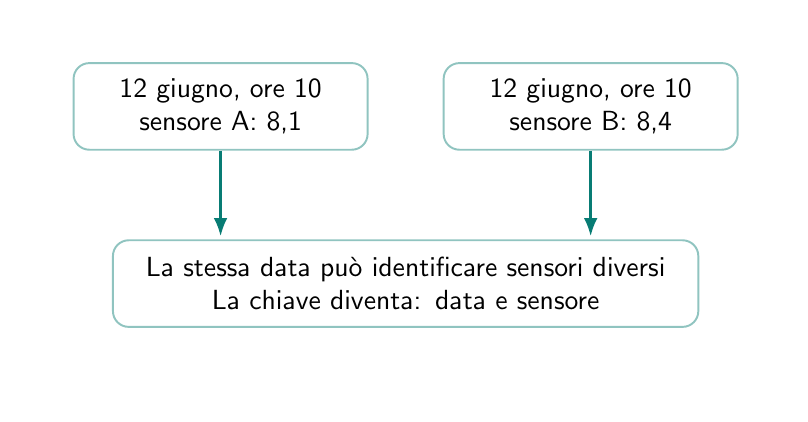
\begin{tikzpicture}[x=1cm,y=1cm]
\path[use as bounding box](-.15,-.15) rectangle(9.4,4.5);
\node[pFlow,text width=3.5cm] (a) at(2.3,3.5){12 giugno, ore 10\\sensore A: 8,1};\node[pFlow,text width=3.5cm] (b) at(7,3.5){12 giugno, ore 10\\sensore B: 8,4};\node[pFlow,text width=7.2cm] (c) at(4.65,1.25){La stessa data può identificare sensori diversi\\La chiave diventa: data e sensore};\draw[pEdge](a.south)--(2.3,2)--(2.3,1.85);\draw[pEdge](b.south)--(7,2)--(7,1.85);
\end{tikzpicture}\PBody{Repliche, sensori diversi ed errori di registrazione possono condividere una data. La regola di aggregazione dipende dalla loro origine.}
\end{minipage}%
\end{lrbox}
\typeout{FULLBOX:011:L:\the\ht\PilotLeftBox:\the\dp\PilotLeftBox}
\begin{lrbox}{\PilotRightBox}%
\begin{minipage}[t]{7.55cm}\raggedright\color{Ink}\fontsize{11.3}{14.8}\selectfont
\PCode{R · isolare i duplicati}{011_duplicati.R}\vspace{3mm}\PInfo{Eliminare una riga prima di identificarne il ruolo può cancellare una misura valida.}
\end{minipage}%
\end{lrbox}
\typeout{FULLBOX:011:R:\the\ht\PilotRightBox:\the\dp\PilotRightBox}
\begin{tikzpicture}[remember picture,overlay]
\PilotChrome{Le date duplicate richiedono una spiegazione}{I · TEMPO E CALENDARIO}{11}{La chiave che identifica un’osservazione può comprendere più campi oltre alla data.}
\node[anchor=north west,inner sep=0] at([xshift=0.96cm,yshift=-2.13cm]current page.north west){\usebox{\PilotLeftBox}};
\node[anchor=north west,inner sep=0] at([xshift=11.52cm,yshift=-2.13cm]current page.north west){\usebox{\PilotRightBox}};
\end{tikzpicture}\end{frame}

\begin{frame}[plain]\hypertarget{slide12}{}
\bookmark[level=1,page=12]{La griglia rende espliciti i mesi attesi}
\begin{lrbox}{\PilotLeftBox}%
\begin{minipage}[t]{10.05cm}\raggedright\color{Ink}\fontsize{11.3}{14.8}\selectfont
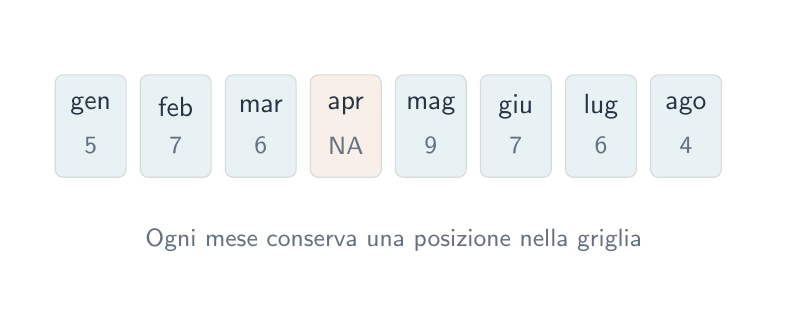
\begin{tikzpicture}[x=1cm,y=1cm]
\path[use as bounding box](-.15,-.15) rectangle(9.4,3.3);
\filldraw[fill=GeoA!10,draw=Rule,rounded corners=1mm](0.2,1.4)rectangle(1.1,2.7);\node[pLabel] at(0.65,2.3){gen};\node[pNote] at(0.65,1.8){5};\filldraw[fill=GeoA!10,draw=Rule,rounded corners=1mm](1.28,1.4)rectangle(2.18,2.7);\node[pLabel] at(1.73,2.3){feb};\node[pNote] at(1.73,1.8){7};\filldraw[fill=GeoA!10,draw=Rule,rounded corners=1mm](2.36,1.4)rectangle(3.2600000000000002,2.7);\node[pLabel] at(2.81,2.3){mar};\node[pNote] at(2.81,1.8){6};\filldraw[fill=GeoB!12,draw=Rule,rounded corners=1mm](3.44,1.4)rectangle(4.34,2.7);\node[pLabel] at(3.89,2.3){apr};\node[pNote] at(3.89,1.8){NA};\filldraw[fill=GeoA!10,draw=Rule,rounded corners=1mm](4.5200000000000005,1.4)rectangle(5.420000000000001,2.7);\node[pLabel] at(4.970000000000001,2.3){mag};\node[pNote] at(4.970000000000001,1.8){9};\filldraw[fill=GeoA!10,draw=Rule,rounded corners=1mm](5.6000000000000005,1.4)rectangle(6.500000000000001,2.7);\node[pLabel] at(6.050000000000001,2.3){giu};\node[pNote] at(6.050000000000001,1.8){7};\filldraw[fill=GeoA!10,draw=Rule,rounded corners=1mm](6.680000000000001,1.4)rectangle(7.580000000000001,2.7);\node[pLabel] at(7.130000000000001,2.3){lug};\node[pNote] at(7.130000000000001,1.8){6};\filldraw[fill=GeoA!10,draw=Rule,rounded corners=1mm](7.760000000000001,1.4)rectangle(8.66,2.7);\node[pLabel] at(8.21,2.3){ago};\node[pNote] at(8.21,1.8){4};\node[pNote] at(4.5,.6){Ogni mese conserva una posizione nella griglia};
\end{tikzpicture}\PBody{Il confronto con una griglia completa distingue una riga assente da una riga presente con misura mancante.}
\end{minipage}%
\end{lrbox}
\typeout{FULLBOX:012:L:\the\ht\PilotLeftBox:\the\dp\PilotLeftBox}
\begin{lrbox}{\PilotRightBox}%
\begin{minipage}[t]{7.55cm}\raggedright\color{Ink}\fontsize{11.3}{14.8}\selectfont
\PCode{R · ricostruire il calendario}{012_griglia.R}\PSmall{La chiave data deve essere univoca prima del merge. In caso contrario, una data può generare più righe.}
\end{minipage}%
\end{lrbox}
\typeout{FULLBOX:012:R:\the\ht\PilotRightBox:\the\dp\PilotRightBox}
\begin{tikzpicture}[remember picture,overlay]
\PilotChrome{La griglia rende espliciti i mesi attesi}{I · TEMPO E CALENDARIO}{12}{La griglia attesa è una scelta esplicita fondata sul calendario e sul protocollo di osservazione.}
\node[anchor=north west,inner sep=0] at([xshift=0.96cm,yshift=-2.13cm]current page.north west){\usebox{\PilotLeftBox}};
\node[anchor=north west,inner sep=0] at([xshift=11.52cm,yshift=-2.13cm]current page.north west){\usebox{\PilotRightBox}};
\end{tikzpicture}\end{frame}

\begin{frame}[plain]\hypertarget{slide13}{}
\bookmark[level=1,page=13]{ts assegna una frequenza alla successione}
\begin{lrbox}{\PilotLeftBox}%
\begin{minipage}[t]{10.05cm}\raggedright\color{Ink}\fontsize{11.3}{14.8}\selectfont
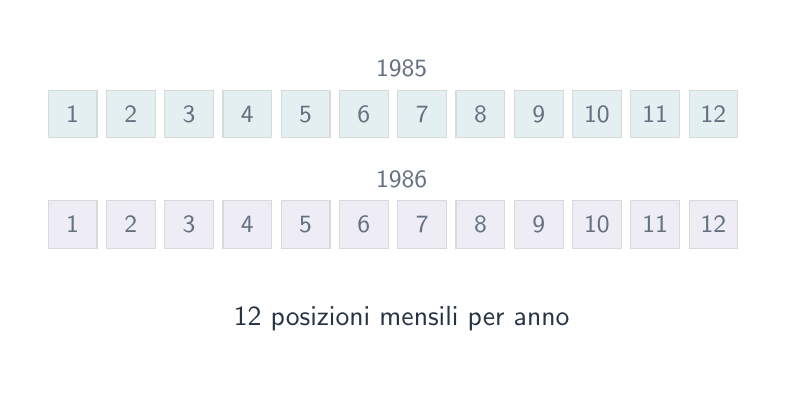
\begin{tikzpicture}[x=1cm,y=1cm]
\path[use as bounding box](-.15,-.15) rectangle(9.4,4.2);
\filldraw[fill=GeoA!12,draw=Rule](0.10999999999999999,2.8000000000000003)rectangle(0.73,3.4);\node[pNote] at(0.42,3.1){1};\filldraw[fill=GeoA!12,draw=Rule](0.8499999999999999,2.8000000000000003)rectangle(1.47,3.4);\node[pNote] at(1.16,3.1){2};\filldraw[fill=GeoA!12,draw=Rule](1.5899999999999999,2.8000000000000003)rectangle(2.21,3.4);\node[pNote] at(1.9,3.1){3};\filldraw[fill=GeoA!12,draw=Rule](2.3299999999999996,2.8000000000000003)rectangle(2.9499999999999997,3.4);\node[pNote] at(2.6399999999999997,3.1){4};\filldraw[fill=GeoA!12,draw=Rule](3.07,2.8000000000000003)rectangle(3.69,3.4);\node[pNote] at(3.38,3.1){5};\filldraw[fill=GeoA!12,draw=Rule](3.81,2.8000000000000003)rectangle(4.43,3.4);\node[pNote] at(4.12,3.1){6};\filldraw[fill=GeoA!12,draw=Rule](4.55,2.8000000000000003)rectangle(5.169999999999999,3.4);\node[pNote] at(4.859999999999999,3.1){7};\filldraw[fill=GeoA!12,draw=Rule](5.29,2.8000000000000003)rectangle(5.909999999999999,3.4);\node[pNote] at(5.6,3.1){8};\filldraw[fill=GeoA!12,draw=Rule](6.03,2.8000000000000003)rectangle(6.6499999999999995,3.4);\node[pNote] at(6.34,3.1){9};\filldraw[fill=GeoA!12,draw=Rule](6.7700000000000005,2.8000000000000003)rectangle(7.39,3.4);\node[pNote] at(7.08,3.1){10};\filldraw[fill=GeoA!12,draw=Rule](7.510000000000001,2.8000000000000003)rectangle(8.13,3.4);\node[pNote] at(7.82,3.1){11};\filldraw[fill=GeoA!12,draw=Rule](8.25,2.8000000000000003)rectangle(8.870000000000001,3.4);\node[pNote] at(8.56,3.1){12};\node[pNote] at(4.6,3.68){1985};\filldraw[fill=GeoC!12,draw=Rule](0.10999999999999999,1.4000000000000001)rectangle(0.73,2.0);\node[pNote] at(0.42,1.7000000000000002){1};\filldraw[fill=GeoC!12,draw=Rule](0.8499999999999999,1.4000000000000001)rectangle(1.47,2.0);\node[pNote] at(1.16,1.7000000000000002){2};\filldraw[fill=GeoC!12,draw=Rule](1.5899999999999999,1.4000000000000001)rectangle(2.21,2.0);\node[pNote] at(1.9,1.7000000000000002){3};\filldraw[fill=GeoC!12,draw=Rule](2.3299999999999996,1.4000000000000001)rectangle(2.9499999999999997,2.0);\node[pNote] at(2.6399999999999997,1.7000000000000002){4};\filldraw[fill=GeoC!12,draw=Rule](3.07,1.4000000000000001)rectangle(3.69,2.0);\node[pNote] at(3.38,1.7000000000000002){5};\filldraw[fill=GeoC!12,draw=Rule](3.81,1.4000000000000001)rectangle(4.43,2.0);\node[pNote] at(4.12,1.7000000000000002){6};\filldraw[fill=GeoC!12,draw=Rule](4.55,1.4000000000000001)rectangle(5.169999999999999,2.0);\node[pNote] at(4.859999999999999,1.7000000000000002){7};\filldraw[fill=GeoC!12,draw=Rule](5.29,1.4000000000000001)rectangle(5.909999999999999,2.0);\node[pNote] at(5.6,1.7000000000000002){8};\filldraw[fill=GeoC!12,draw=Rule](6.03,1.4000000000000001)rectangle(6.6499999999999995,2.0);\node[pNote] at(6.34,1.7000000000000002){9};\filldraw[fill=GeoC!12,draw=Rule](6.7700000000000005,1.4000000000000001)rectangle(7.39,2.0);\node[pNote] at(7.08,1.7000000000000002){10};\filldraw[fill=GeoC!12,draw=Rule](7.510000000000001,1.4000000000000001)rectangle(8.13,2.0);\node[pNote] at(7.82,1.7000000000000002){11};\filldraw[fill=GeoC!12,draw=Rule](8.25,1.4000000000000001)rectangle(8.870000000000001,2.0);\node[pNote] at(8.56,1.7000000000000002){12};\node[pNote] at(4.6,2.2800000000000002){1986};\node[pLabel] at(4.6,.5){12 posizioni mensili per anno};
\end{tikzpicture}\[t_i=1985+\frac{i-1}{12},\qquad i=1,\ldots,204.\]
\end{minipage}%
\end{lrbox}
\typeout{FULLBOX:013:L:\the\ht\PilotLeftBox:\the\dp\PilotLeftBox}
\begin{lrbox}{\PilotRightBox}%
\begin{minipage}[t]{7.55cm}\raggedright\color{Ink}\fontsize{11.3}{14.8}\selectfont
\PCode{R · costruire la serie mensile}{013_ts.R}\PInfo{ts memorizza inizio e frequenza. La tabella con le date civili resta necessaria per ricondurre ogni risultato al calendario.}
\end{minipage}%
\end{lrbox}
\typeout{FULLBOX:013:R:\the\ht\PilotRightBox:\the\dp\PilotRightBox}
\begin{tikzpicture}[remember picture,overlay]
\PilotChrome{ts assegna una frequenza alla successione}{I · TEMPO E CALENDARIO}{13}{frequency = 12 dichiara dodici passi per anno. Non verifica da sola la regolarità del file.}
\node[anchor=north west,inner sep=0] at([xshift=0.96cm,yshift=-2.13cm]current page.north west){\usebox{\PilotLeftBox}};
\node[anchor=north west,inner sep=0] at([xshift=11.52cm,yshift=-2.13cm]current page.north west){\usebox{\PilotRightBox}};
\end{tikzpicture}\end{frame}

\begin{frame}[plain]\hypertarget{slide14}{}
\bookmark[level=1,page=14]{Il segmento completo comprende 204 mesi}
\begin{lrbox}{\PilotLeftBox}%
\begin{minipage}[t]{10.05cm}\raggedright\color{Ink}\fontsize{11.3}{14.8}\selectfont
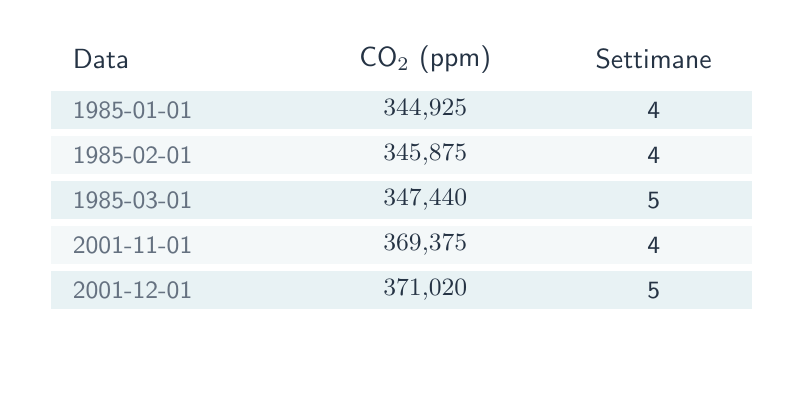
\begin{tikzpicture}[x=1cm,y=1cm]
\path[use as bounding box](-.15,-.15) rectangle(9.4,4.2);
\node[pLabel,anchor=west] at(.3,3.8){Data};\node[pLabel] at(4.9,3.8){CO$_2$ (ppm)};\node[pLabel] at(7.8,3.8){Settimane};\fill[GeoA!10](.15,2.91) rectangle(9.05,3.3899999999999997);\node[pNote,anchor=west] at(.3,3.15){1985-01-01};\node[pNote,text=Ink] at(4.9,3.15){$ 344{,}925 $};\node[pNote,text=Ink] at(7.8,3.15){4};\fill[GeoA!5](.15,2.34) rectangle(9.05,2.8200000000000003);\node[pNote,anchor=west] at(.3,2.58){1985-02-01};\node[pNote,text=Ink] at(4.9,2.58){$ 345{,}875 $};\node[pNote,text=Ink] at(7.8,2.58){4};\fill[GeoA!10](.15,1.7699999999999998) rectangle(9.05,2.25);\node[pNote,anchor=west] at(.3,2.01){1985-03-01};\node[pNote,text=Ink] at(4.9,2.01){$ 347{,}440 $};\node[pNote,text=Ink] at(7.8,2.01){5};\fill[GeoA!5](.15,1.2) rectangle(9.05,1.68);\node[pNote,anchor=west] at(.3,1.44){2001-11-01};\node[pNote,text=Ink] at(4.9,1.44){$ 369{,}375 $};\node[pNote,text=Ink] at(7.8,1.44){4};\fill[GeoA!10](.15,0.6300000000000001) rectangle(9.05,1.11);\node[pNote,anchor=west] at(.3,0.8700000000000001){2001-12-01};\node[pNote,text=Ink] at(4.9,0.8700000000000001){$ 371{,}020 $};\node[pNote,text=Ink] at(7.8,0.8700000000000001){5};
\end{tikzpicture}\PSmall{Gennaio 1985–dicembre 2001: 17 anni, 204 mesi, nessun valore mancante.}
\end{minipage}%
\end{lrbox}
\typeout{FULLBOX:014:L:\the\ht\PilotLeftBox:\the\dp\PilotLeftBox}
\begin{lrbox}{\PilotRightBox}%
\begin{minipage}[t]{7.55cm}\raggedright\color{Ink}\fontsize{11.3}{14.8}\selectfont
\PCode{R · verificare prima del calcolo}{014_controllo_ts.R}\PBody{Useremo questo segmento per confrontare trasformazioni. Il calendario sarà mantenuto anche quando le differenze accorciano la serie.}
\end{minipage}%
\end{lrbox}
\typeout{FULLBOX:014:R:\the\ht\PilotRightBox:\the\dp\PilotRightBox}
\begin{tikzpicture}[remember picture,overlay]
\PilotChrome{Il segmento completo comprende 204 mesi}{I · TEMPO E CALENDARIO}{14}{Un controllo esplicito del calendario rende verificabili le trasformazioni successive.}
\node[anchor=north west,inner sep=0] at([xshift=0.96cm,yshift=-2.13cm]current page.north west){\usebox{\PilotLeftBox}};
\node[anchor=north west,inner sep=0] at([xshift=11.52cm,yshift=-2.13cm]current page.north west){\usebox{\PilotRightBox}};
\end{tikzpicture}\end{frame}

\begin{frame}[plain]\hypertarget{slide15}{}
\bookmark[level=0,page=15]{Aggregazione e risoluzione}
\bookmark[level=1,page=15]{Ogni media porta con sé la copertura}
\begin{lrbox}{\PilotLeftBox}%
\begin{minipage}[t]{10.05cm}\raggedright\color{Ink}\fontsize{11.3}{14.8}\selectfont
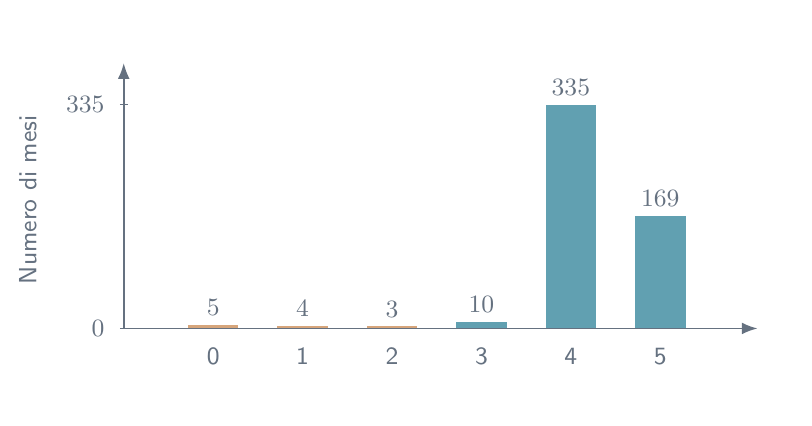
\begin{tikzpicture}[x=1cm,y=1cm]
\path[use as bounding box](-.3,-.2) rectangle(9.299999999999999,4.5);
\draw[pAxis](0.92,0.68)--(8.969999999999999,0.68);
\draw[pAxis](0.92,0.68)--(0.92,4.050000000000001);
\draw[Muted](0.87,0.6800)--(0.9700000000000001,0.6800);\node[pNote,anchor=east] at(0.8,0.6800){$0$};
\draw[Muted](0.87,3.5235)--(0.9700000000000001,3.5235);\node[pNote,anchor=east] at(0.8,3.5235){$335$};
\node[pNote] at(4.895,0.09000000000000008){};
\node[pNote,rotate=90] at(-.3,2.3150000000000004){Numero di mesi};
\fill[GeoB!70](1.7357142857142855,0.6800)rectangle(2.3757142857142854,0.7224);\node[pNote] at(2.0557142857142856,0.9424){$ 5 $};\node[pNote] at(2.0557142857142856,.32){0};
\fill[GeoB!70](2.871428571428571,0.6800)rectangle(3.5114285714285707,0.7140);\node[pNote] at(3.191428571428571,0.9340){$ 4 $};\node[pNote] at(3.191428571428571,.32){1};
\fill[GeoB!70](4.007142857142856,0.6800)rectangle(4.647142857142857,0.7055);\node[pNote] at(4.3271428571428565,0.9255){$ 3 $};\node[pNote] at(4.3271428571428565,.32){2};
\fill[GeoA!70](5.1428571428571415,0.6800)rectangle(5.782857142857142,0.7649);\node[pNote] at(5.462857142857142,0.9849){$ 10 $};\node[pNote] at(5.462857142857142,.32){3};
\fill[GeoA!70](6.278571428571428,0.6800)rectangle(6.918571428571428,3.5235);\node[pNote] at(6.598571428571428,3.7435){$ 335 $};\node[pNote] at(6.598571428571428,.32){4};
\fill[GeoA!70](7.414285714285713,0.6800)rectangle(8.054285714285713,2.1145);\node[pNote] at(7.734285714285713,2.3345){$ 169 $};\node[pNote] at(7.734285714285713,.32){5};
\end{tikzpicture}\PSmall{Archivio mensile completo: numero di mesi per quantità di valori settimanali disponibili.}
\end{minipage}%
\end{lrbox}
\typeout{FULLBOX:015:L:\the\ht\PilotLeftBox:\the\dp\PilotLeftBox}
\begin{lrbox}{\PilotRightBox}%
\begin{minipage}[t]{7.55cm}\raggedright\color{Ink}\fontsize{11.3}{14.8}\selectfont
\[\bar x_m=\frac{1}{n_m}\sum_{\substack{i\in m\\x_i\ \mathrm{osservato}}}x_i.\]
\PBody{$n_m$ conta le osservazioni disponibili nel mese. Quando $n_m=0$, la media rimane assente.}
\vspace{3mm}
\PInfo{Un conteggio alto non garantisce una copertura uniforme: anche la posizione delle assenze nel mese può influenzare il risultato.}
\vspace{3mm}
\PBody{Nel segmento 1985–2001 ogni mese ha almeno tre osservazioni settimanali. L’archivio completo ha copertura più variabile.}
\end{minipage}%
\end{lrbox}
\typeout{FULLBOX:015:R:\the\ht\PilotRightBox:\the\dp\PilotRightBox}
\begin{tikzpicture}[remember picture,overlay]
\PilotChrome{Ogni media porta con sé la copertura}{II · AGGREGAZIONE E RISOLUZIONE}{15}{Una media senza informazioni sulla copertura può nascondere periodi osservati in modo disomogeneo.}
\node[anchor=north west,inner sep=0] at([xshift=0.96cm,yshift=-2.13cm]current page.north west){\usebox{\PilotLeftBox}};
\node[anchor=north west,inner sep=0] at([xshift=11.52cm,yshift=-2.13cm]current page.north west){\usebox{\PilotRightBox}};
\end{tikzpicture}\end{frame}

\begin{frame}[plain]\hypertarget{slide16}{}
\bookmark[level=1,page=16]{Dal valore settimanale alla media mensile}
\begin{lrbox}{\PilotLeftBox}%
\begin{minipage}[t]{10.05cm}\raggedright\color{Ink}\fontsize{11.3}{14.8}\selectfont
\PLabel{Una regola riproducibile}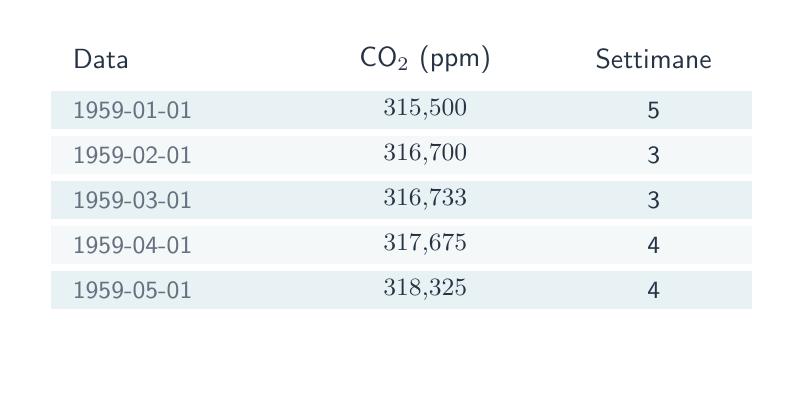
\begin{tikzpicture}[x=1cm,y=1cm]
\path[use as bounding box](-.15,-.15) rectangle(9.4,4.2);
\node[pLabel,anchor=west] at(.3,3.8){Data};\node[pLabel] at(4.9,3.8){CO$_2$ (ppm)};\node[pLabel] at(7.8,3.8){Settimane};\fill[GeoA!10](.15,2.91) rectangle(9.05,3.3899999999999997);\node[pNote,anchor=west] at(.3,3.15){1959-01-01};\node[pNote,text=Ink] at(4.9,3.15){$ 315{,}500 $};\node[pNote,text=Ink] at(7.8,3.15){5};\fill[GeoA!5](.15,2.34) rectangle(9.05,2.8200000000000003);\node[pNote,anchor=west] at(.3,2.58){1959-02-01};\node[pNote,text=Ink] at(4.9,2.58){$ 316{,}700 $};\node[pNote,text=Ink] at(7.8,2.58){3};\fill[GeoA!10](.15,1.7699999999999998) rectangle(9.05,2.25);\node[pNote,anchor=west] at(.3,2.01){1959-03-01};\node[pNote,text=Ink] at(4.9,2.01){$ 316{,}733 $};\node[pNote,text=Ink] at(7.8,2.01){3};\fill[GeoA!5](.15,1.2) rectangle(9.05,1.68);\node[pNote,anchor=west] at(.3,1.44){1959-04-01};\node[pNote,text=Ink] at(4.9,1.44){$ 317{,}675 $};\node[pNote,text=Ink] at(7.8,1.44){4};\fill[GeoA!10](.15,0.6300000000000001) rectangle(9.05,1.11);\node[pNote,anchor=west] at(.3,0.8700000000000001){1959-05-01};\node[pNote,text=Ink] at(4.9,0.8700000000000001){$ 318{,}325 $};\node[pNote,text=Ink] at(7.8,0.8700000000000001){4};
\end{tikzpicture}\PBody{Il raggruppamento usa il mese della data. Una settimana che attraversa due mesi non viene suddivisa fra loro.}
\end{minipage}%
\end{lrbox}
\typeout{FULLBOX:016:L:\the\ht\PilotLeftBox:\the\dp\PilotLeftBox}
\begin{lrbox}{\PilotRightBox}%
\begin{minipage}[t]{7.55cm}\raggedright\color{Ink}\fontsize{11.3}{14.8}\selectfont
\PCode{R · aggregare con una regola esplicita}{016_aggregare.R}\PSmall{La condizione all(is.na(v)) evita di restituire NaN per un mese completamente privo di valori.}
\end{minipage}%
\end{lrbox}
\typeout{FULLBOX:016:R:\the\ht\PilotRightBox:\the\dp\PilotRightBox}
\begin{tikzpicture}[remember picture,overlay]
\PilotChrome{Dal valore settimanale alla media mensile}{II · AGGREGAZIONE E RISOLUZIONE}{16}{La convenzione di assegnazione al mese appartiene alla definizione del dato derivato.}
\node[anchor=north west,inner sep=0] at([xshift=0.96cm,yshift=-2.13cm]current page.north west){\usebox{\PilotLeftBox}};
\node[anchor=north west,inner sep=0] at([xshift=11.52cm,yshift=-2.13cm]current page.north west){\usebox{\PilotRightBox}};
\end{tikzpicture}\end{frame}

\begin{frame}[plain]\hypertarget{slide17}{}
\bookmark[level=1,page=17]{La ricostruzione si confronta con il file}
\begin{lrbox}{\PilotLeftBox}%
\begin{minipage}[t]{10.05cm}\raggedright\color{Ink}\fontsize{11.3}{14.8}\selectfont
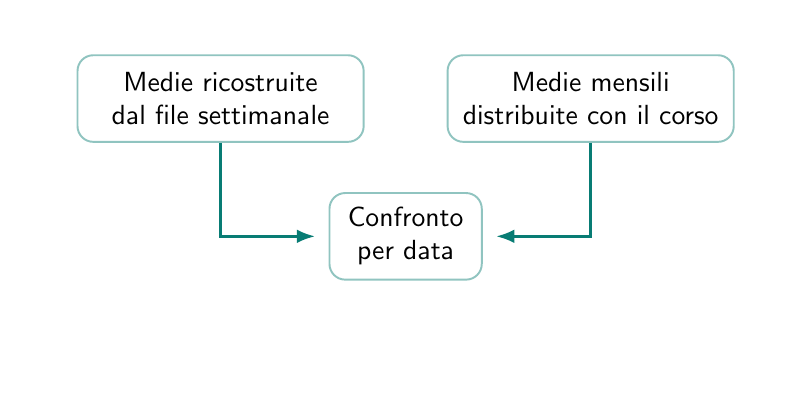
\begin{tikzpicture}[x=1cm,y=1cm]
\path[use as bounding box](-.15,-.15) rectangle(9.4,4.2);
\node[pFlow,text width=3.4cm] (a) at(2.3,3.3){Medie ricostruite\\dal file settimanale};\node[pFlow,text width=3.4cm] (b) at(7,3.3){Medie mensili\\distribuite con il corso};\draw[pEdge](a.south)--(2.3,1.55)--(3.5,1.55);\draw[pEdge](b.south)--(7,1.55)--(5.8,1.55);\node[pFlow,text width=1.7cm] at(4.65,1.55){Confronto\\per data};
\end{tikzpicture}\PBody{La corrispondenza è verificata dopo l’allineamento delle date. La tolleranza riflette gli arrotondamenti del CSV.}
\end{minipage}%
\end{lrbox}
\typeout{FULLBOX:017:L:\the\ht\PilotLeftBox:\the\dp\PilotLeftBox}
\begin{lrbox}{\PilotRightBox}%
\begin{minipage}[t]{7.55cm}\raggedright\color{Ink}\fontsize{11.3}{14.8}\selectfont
\PCode{R · verificare la ricostruzione}{017_confronto.R}
\end{minipage}%
\end{lrbox}
\typeout{FULLBOX:017:R:\the\ht\PilotRightBox:\the\dp\PilotRightBox}
\begin{tikzpicture}[remember picture,overlay]
\PilotChrome{La ricostruzione si confronta con il file}{II · AGGREGAZIONE E RISOLUZIONE}{17}{Il confronto numerico richiede le stesse date, la stessa regola e una tolleranza dichiarata.}
\node[anchor=north west,inner sep=0] at([xshift=0.96cm,yshift=-2.13cm]current page.north west){\usebox{\PilotLeftBox}};
\node[anchor=north west,inner sep=0] at([xshift=11.52cm,yshift=-2.13cm]current page.north west){\usebox{\PilotRightBox}};
\end{tikzpicture}\end{frame}

\begin{frame}[plain]\hypertarget{slide18}{}
\bookmark[level=1,page=18]{La media delle medie cambia i pesi}
\begin{lrbox}{\PilotLeftBox}%
\begin{minipage}[t]{10.05cm}\raggedright\color{Ink}\fontsize{11.3}{14.8}\selectfont
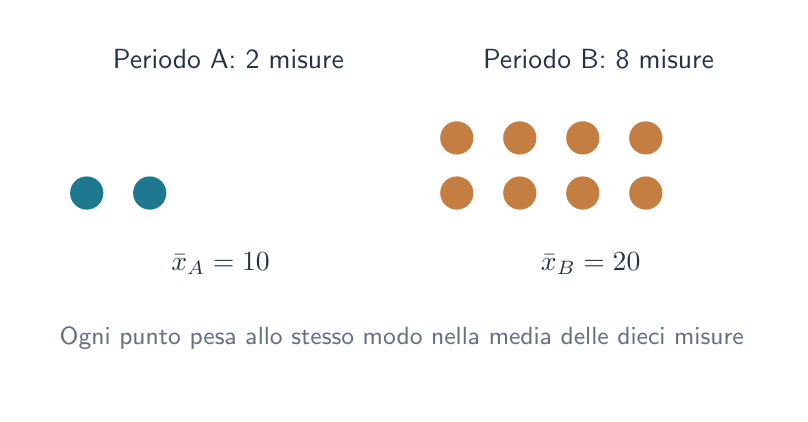
\begin{tikzpicture}[x=1cm,y=1cm]
\path[use as bounding box](-.15,-.15) rectangle(9.4,4.5);
\node[pLabel] at(2.4,4.1){Periodo A: 2 misure};\fill[GeoA](0.6,2.4)circle(6pt);\fill[GeoA](1.4,2.4)circle(6pt);\node[pLabel] at(2.3,1.5){$\bar x_A=10$};\node[pLabel] at(7.1,4.1){Periodo B: 8 misure};\fill[GeoB](5.3,2.4)circle(6pt);\fill[GeoB](6.1,2.4)circle(6pt);\fill[GeoB](6.9,2.4)circle(6pt);\fill[GeoB](7.7,2.4)circle(6pt);\fill[GeoB](5.3,3.0999999999999996)circle(6pt);\fill[GeoB](6.1,3.0999999999999996)circle(6pt);\fill[GeoB](6.9,3.0999999999999996)circle(6pt);\fill[GeoB](7.7,3.0999999999999996)circle(6pt);\node[pLabel] at(7.0,1.5){$\bar x_B=20$};\node[pNote] at(4.6,.55){Ogni punto pesa allo stesso modo nella media delle dieci misure};
\end{tikzpicture}
\end{minipage}%
\end{lrbox}
\typeout{FULLBOX:018:L:\the\ht\PilotLeftBox:\the\dp\PilotLeftBox}
\begin{lrbox}{\PilotRightBox}%
\begin{minipage}[t]{7.55cm}\raggedright\color{Ink}\fontsize{11.3}{14.8}\selectfont
\PBody{Due periodi hanno medie 10 e 20. Il primo contiene due misure, il secondo otto.}
\vspace{3mm}
\[\bar x_{\rm periodi}=\frac{10+20}{2}=15.\]
\[\bar x_{\rm misure}=\frac{2\cdot10+8\cdot20}{10}=18.\]
\PInfo{La prima quantità pesa allo stesso modo i periodi. La seconda pesa allo stesso modo le dieci misure disponibili.}
\end{minipage}%
\end{lrbox}
\typeout{FULLBOX:018:R:\the\ht\PilotRightBox:\the\dp\PilotRightBox}
\begin{tikzpicture}[remember picture,overlay]
\PilotChrome{La media delle medie cambia i pesi}{II · AGGREGAZIONE E RISOLUZIONE}{18}{La media dei periodi e la media delle misure rispondono a domande diverse quando le numerosità cambiano.}
\node[anchor=north west,inner sep=0] at([xshift=0.96cm,yshift=-2.13cm]current page.north west){\usebox{\PilotLeftBox}};
\node[anchor=north west,inner sep=0] at([xshift=11.52cm,yshift=-2.13cm]current page.north west){\usebox{\PilotRightBox}};
\end{tikzpicture}\end{frame}

\begin{frame}[plain]\hypertarget{slide19}{}
\bookmark[level=1,page=19]{I pesi dichiarano la quantità stimata}
\begin{lrbox}{\PilotLeftBox}%
\begin{minipage}[t]{10.05cm}\raggedright\color{Ink}\fontsize{11.3}{14.8}\selectfont
\[\bar x_{\rm misure}=\frac{\sum_{m=1}^{M}n_m\bar x_m}{\sum_{m=1}^{M}n_m}.\]
\[\bar x_{\rm periodi}=\frac{1}{M}\sum_{m=1}^{M}\bar x_m.\]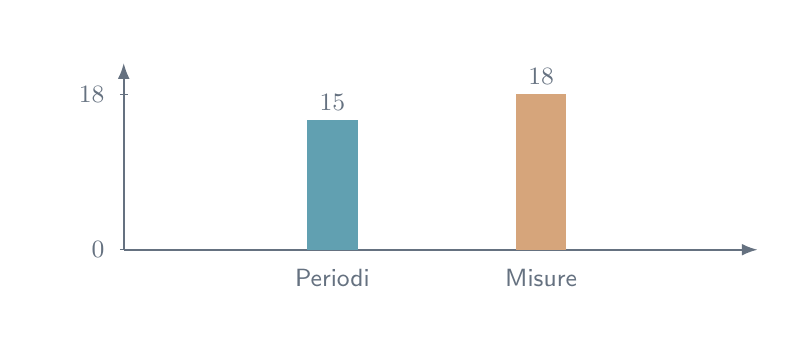
\begin{tikzpicture}[x=1cm,y=1cm]
\path[use as bounding box](-.3,-.2) rectangle(9.299999999999999,3.5);
\draw[pAxis](0.92,0.68)--(8.969999999999999,0.68);
\draw[pAxis](0.92,0.68)--(0.92,3.0500000000000003);
\draw[Muted](0.87,0.6800)--(0.9700000000000001,0.6800);\node[pNote,anchor=east] at(0.8,0.6800){$0$};
\draw[Muted](0.87,2.6539)--(0.9700000000000001,2.6539);\node[pNote,anchor=east] at(0.8,2.6539){$18$};
\node[pNote] at(4.895,0.09000000000000008){};
\fill[GeoA!70](3.2499999999999996,0.6800)rectangle(3.8899999999999992,2.3249);\node[pNote] at(3.5699999999999994,2.5449){$ 15 $};\node[pNote] at(3.5699999999999994,.32){Periodi};
\fill[GeoB!70](5.899999999999999,0.6800)rectangle(6.539999999999999,2.6539);\node[pNote] at(6.219999999999999,2.8739){$ 18 $};\node[pNote] at(6.219999999999999,.32){Misure};
\end{tikzpicture}
\end{minipage}%
\end{lrbox}
\typeout{FULLBOX:019:L:\the\ht\PilotLeftBox:\the\dp\PilotLeftBox}
\begin{lrbox}{\PilotRightBox}%
\begin{minipage}[t]{7.55cm}\raggedright\color{Ink}\fontsize{11.3}{14.8}\selectfont
\PCode{R · calcolare le due medie}{019_pesi.R}\PBody{Numerosità uguali fanno coincidere le due formule. Possono coincidere anche in casi particolari, per esempio se tutte le medie dei periodi sono uguali.}
\end{minipage}%
\end{lrbox}
\typeout{FULLBOX:019:R:\the\ht\PilotRightBox:\the\dp\PilotRightBox}
\begin{tikzpicture}[remember picture,overlay]
\PilotChrome{I pesi dichiarano la quantità stimata}{II · AGGREGAZIONE E RISOLUZIONE}{19}{Prima di calcolare una media complessiva bisogna scegliere cosa riceve uguale peso.}
\node[anchor=north west,inner sep=0] at([xshift=0.96cm,yshift=-2.13cm]current page.north west){\usebox{\PilotLeftBox}};
\node[anchor=north west,inner sep=0] at([xshift=11.52cm,yshift=-2.13cm]current page.north west){\usebox{\PilotRightBox}};
\end{tikzpicture}\end{frame}

\begin{frame}[plain]\hypertarget{slide20}{}
\bookmark[level=1,page=20]{Intervalli diversi possono richiedere durate}
\begin{lrbox}{\PilotLeftBox}%
\begin{minipage}[t]{10.05cm}\raggedright\color{Ink}\fontsize{11.3}{14.8}\selectfont
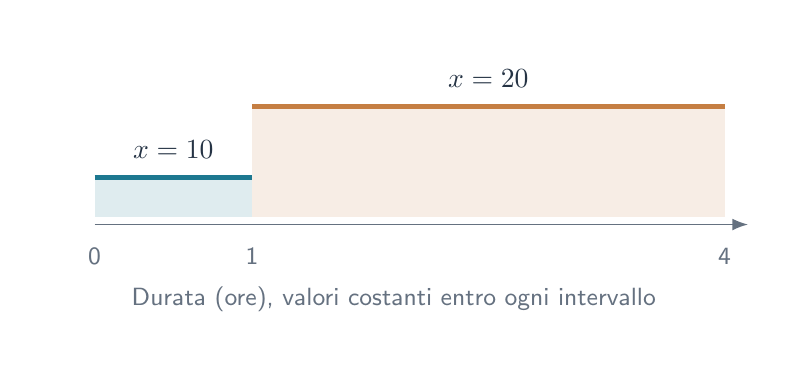
\begin{tikzpicture}[x=1cm,y=1cm]
\path[use as bounding box](-.15,-.15) rectangle(9.4,3.8);
\fill[GeoA!14](0.7,1.4)rectangle(2.7,1.9);\draw[GeoA,line width=2pt](0.7,1.9)--(2.7,1.9);\node[pLabel] at(1.7,2.25){$x=10$};\fill[GeoB!14](2.7,1.4)rectangle(8.7,2.8);\draw[GeoB,line width=2pt](2.7,2.8)--(8.7,2.8);\node[pLabel] at(5.7,3.15){$x=20$};\draw[pAxis](.7,1.3)--(9,1.3);\node[pNote] at(.7,.9){0};\node[pNote] at(2.7,.9){1};\node[pNote] at(8.7,.9){4};\node[pNote] at(4.5,.35){Durata (ore), valori costanti entro ogni intervallo};
\end{tikzpicture}\[\bar x_{\rm tempo}=\frac{1\cdot10+3\cdot20}{1+3}=17{,}5.\]
\end{minipage}%
\end{lrbox}
\typeout{FULLBOX:020:L:\the\ht\PilotLeftBox:\the\dp\PilotLeftBox}
\begin{lrbox}{\PilotRightBox}%
\begin{minipage}[t]{7.55cm}\raggedright\color{Ink}\fontsize{11.3}{14.8}\selectfont
\PCode{R · pesare per il tempo rappresentato}{020_durate.R}\PInfo{I pesi di durata sono appropriati se il valore rappresenta l’intero intervallo. Misure puntuali irregolari richiedono un modello di interpolazione o integrazione.}
\end{minipage}%
\end{lrbox}
\typeout{FULLBOX:020:R:\the\ht\PilotRightBox:\the\dp\PilotRightBox}
\begin{tikzpicture}[remember picture,overlay]
\PilotChrome{Intervalli diversi possono richiedere durate}{II · AGGREGAZIONE E RISOLUZIONE}{20}{Un peso temporale ha senso soltanto insieme all’ipotesi su ciò che accade fra due misure.}
\node[anchor=north west,inner sep=0] at([xshift=0.96cm,yshift=-2.13cm]current page.north west){\usebox{\PilotLeftBox}};
\node[anchor=north west,inner sep=0] at([xshift=11.52cm,yshift=-2.13cm]current page.north west){\usebox{\PilotRightBox}};
\end{tikzpicture}\end{frame}

\begin{frame}[plain]\hypertarget{slide21}{}
\bookmark[level=1,page=21]{Somma, media e massimo cambiano la domanda}
\begin{lrbox}{\PilotLeftBox}%
\begin{minipage}[t]{10.05cm}\raggedright\color{Ink}\fontsize{11.3}{14.8}\selectfont
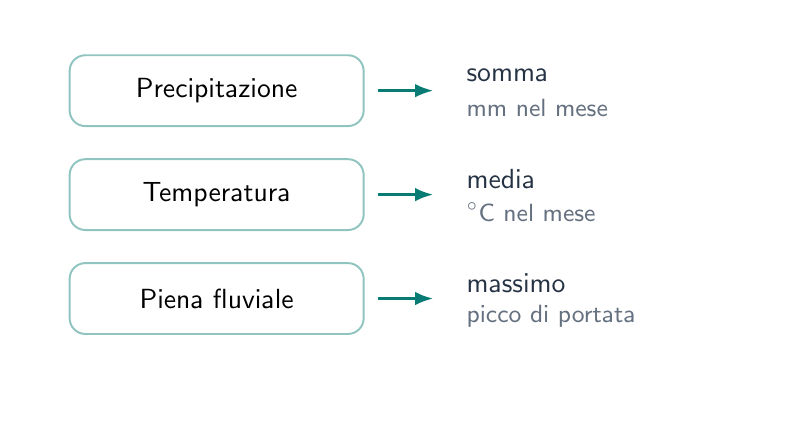
\begin{tikzpicture}[x=1cm,y=1cm]
\path[use as bounding box](-.15,-.15) rectangle(9.4,4.5);
\node[pFlow,text width=3.5cm,minimum height=.9cm] at(2.25,3.7){Precipitazione};\draw[pEdge](4.3,3.7)--(5.0,3.7);\node[pLabel,anchor=west] at(5.3,3.9000000000000004){somma};\node[pNote,anchor=west] at(5.3,3.48){mm nel mese};\node[pFlow,text width=3.5cm,minimum height=.9cm] at(2.25,2.38){Temperatura};\draw[pEdge](4.3,2.38)--(5.0,2.38);\node[pLabel,anchor=west] at(5.3,2.58){media};\node[pNote,anchor=west] at(5.3,2.1599999999999997){$^\circ$C nel mese};\node[pFlow,text width=3.5cm,minimum height=.9cm] at(2.25,1.06){Piena fluviale};\draw[pEdge](4.3,1.06)--(5.0,1.06);\node[pLabel,anchor=west] at(5.3,1.26){massimo};\node[pNote,anchor=west] at(5.3,0.8400000000000001){picco di portata};
\end{tikzpicture}
\end{minipage}%
\end{lrbox}
\typeout{FULLBOX:021:L:\the\ht\PilotLeftBox:\the\dp\PilotLeftBox}
\begin{lrbox}{\PilotRightBox}%
\begin{minipage}[t]{7.55cm}\raggedright\color{Ink}\fontsize{11.3}{14.8}\selectfont
\PCode{R · specificare l’aggregato}{021_operatori.R}\PBody{Una somma con un giorno assente è il totale dei soli giorni osservati. Un massimo su un periodo incompleto può perdere proprio il picco.}
\end{minipage}%
\end{lrbox}
\typeout{FULLBOX:021:R:\the\ht\PilotRightBox:\the\dp\PilotRightBox}
\begin{tikzpicture}[remember picture,overlay]
\PilotChrome{Somma, media e massimo cambiano la domanda}{II · AGGREGAZIONE E RISOLUZIONE}{21}{La gestione delle assenze deve essere coerente con la quantità che l’aggregato intende descrivere.}
\node[anchor=north west,inner sep=0] at([xshift=0.96cm,yshift=-2.13cm]current page.north west){\usebox{\PilotLeftBox}};
\node[anchor=north west,inner sep=0] at([xshift=11.52cm,yshift=-2.13cm]current page.north west){\usebox{\PilotRightBox}};
\end{tikzpicture}\end{frame}

\begin{frame}[plain]\hypertarget{slide22}{}
\bookmark[level=1,page=22]{Aggregare attenua le variazioni rapide}
\begin{lrbox}{\PilotLeftBox}%
\begin{minipage}[t]{10.05cm}\raggedright\color{Ink}\fontsize{11.3}{14.8}\selectfont
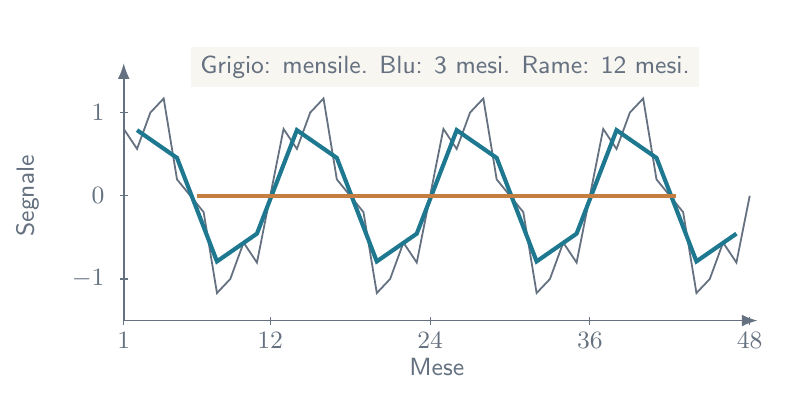
\begin{tikzpicture}[x=1cm,y=1cm]
\path[use as bounding box](-.3,-.2) rectangle(9.299999999999999,4.3999999999999995);
\draw[pAxis](0.92,0.68)--(8.969999999999999,0.68);
\draw[pAxis](0.92,0.68)--(0.92,3.95);
\draw[Muted](0.9200,0.63)--(0.9200,0.7300000000000001);\node[pNote] at(0.9200,0.43000000000000005){$1$};
\draw[Muted](2.7806,0.63)--(2.7806,0.7300000000000001);\node[pNote] at(2.7806,0.43000000000000005){$12$};
\draw[Muted](4.8104,0.63)--(4.8104,0.7300000000000001);\node[pNote] at(4.8104,0.43000000000000005){$24$};
\draw[Muted](6.8402,0.63)--(6.8402,0.7300000000000001);\node[pNote] at(6.8402,0.43000000000000005){$36$};
\draw[Muted](8.8700,0.63)--(8.8700,0.7300000000000001);\node[pNote] at(8.8700,0.43000000000000005){$48$};
\draw[Muted](0.87,1.2083)--(0.9700000000000001,1.2083);\node[pNote,anchor=east] at(0.8,1.2083){$-1$};
\draw[Muted](0.87,2.2650)--(0.9700000000000001,2.2650);\node[pNote,anchor=east] at(0.8,2.2650){$0$};
\draw[Muted](0.87,3.3217)--(0.9700000000000001,3.3217);\node[pNote,anchor=east] at(0.8,3.3217){$1$};
\node[pNote] at(4.895,0.09000000000000008){Mese};
\node[pNote,rotate=90] at(-.3,2.265){Segnale};
\draw[Muted,line width=.65pt] plot coordinates {(0.9200,3.1136) (1.0891,2.8598) (1.2583,3.3217) (1.4274,3.5004) (1.5966,2.4730) (1.7657,2.2650) (1.9349,2.0570) (2.1040,1.0296) (2.2732,1.2083) (2.4423,1.6702) (2.6115,1.4164) (2.7806,2.2650) (2.9498,3.1136) (3.1189,2.8598) (3.2881,3.3217) (3.4572,3.5004) (3.6264,2.4730) (3.7955,2.2650) (3.9647,2.0570) (4.1338,1.0296) (4.3030,1.2083) (4.4721,1.6702) (4.6413,1.4164) (4.8104,2.2650) (4.9796,3.1136) (5.1487,2.8598) (5.3179,3.3217) (5.4870,3.5004) (5.6562,2.4730) (5.8253,2.2650) (5.9945,2.0570) (6.1636,1.0296) (6.3328,1.2083) (6.5019,1.6702) (6.6711,1.4164) (6.8402,2.2650) (7.0094,3.1136) (7.1785,2.8598) (7.3477,3.3217) (7.5168,3.5004) (7.6860,2.4730) (7.8551,2.2650) (8.0243,2.0570) (8.1934,1.0296) (8.3626,1.2083) (8.5317,1.6702) (8.7009,1.4164) (8.8700,2.2650)};
\draw[GeoA,line width=1.5pt] plot coordinates {(1.0891,3.0984) (1.5966,2.7461) (2.1040,1.4316) (2.6115,1.7839) (3.1189,3.0984) (3.6264,2.7461) (4.1338,1.4316) (4.6413,1.7839) (5.1487,3.0984) (5.6562,2.7461) (6.1636,1.4316) (6.6711,1.7839) (7.1785,3.0984) (7.6860,2.7461) (8.1934,1.4316) (8.7009,1.7839)};
\draw[GeoB,line width=1.5pt] plot coordinates {(1.8503,2.2650) (3.8801,2.2650) (5.9099,2.2650) (7.9397,2.2650)};
\node[pNote,fill=Paper] at(5,3.9){Grigio: mensile. Blu: 3 mesi. Rame: 12 mesi.};
\end{tikzpicture}\PSmall{Segnale illustrativo con periodicità di 12 e 3 mesi. Le medie sono calcolate su blocchi disgiunti.}
\end{minipage}%
\end{lrbox}
\typeout{FULLBOX:022:L:\the\ht\PilotLeftBox:\the\dp\PilotLeftBox}
\begin{lrbox}{\PilotRightBox}%
\begin{minipage}[t]{7.55cm}\raggedright\color{Ink}\fontsize{11.3}{14.8}\selectfont
\PCode{R · cambiare la risoluzione}{022_risoluzione.R}\PInfo{Una media annuale può cancellare il ciclo entro l’anno. Dal dato aggregato non si ricostruiscono in generale i valori originali.}
\end{minipage}%
\end{lrbox}
\typeout{FULLBOX:022:R:\the\ht\PilotRightBox:\the\dp\PilotRightBox}
\begin{tikzpicture}[remember picture,overlay]
\PilotChrome{Aggregare attenua le variazioni rapide}{II · AGGREGAZIONE E RISOLUZIONE}{22}{La risoluzione temporale limita le oscillazioni e gli eventi che possiamo riconoscere.}
\node[anchor=north west,inner sep=0] at([xshift=0.96cm,yshift=-2.13cm]current page.north west){\usebox{\PilotLeftBox}};
\node[anchor=north west,inner sep=0] at([xshift=11.52cm,yshift=-2.13cm]current page.north west){\usebox{\PilotRightBox}};
\end{tikzpicture}\end{frame}

\begin{frame}[plain]\hypertarget{slide23}{}
\bookmark[level=1,page=23]{Un campionamento rado può nascondere un ciclo}
\begin{lrbox}{\PilotLeftBox}%
\begin{minipage}[t]{10.05cm}\raggedright\color{Ink}\fontsize{11.3}{14.8}\selectfont
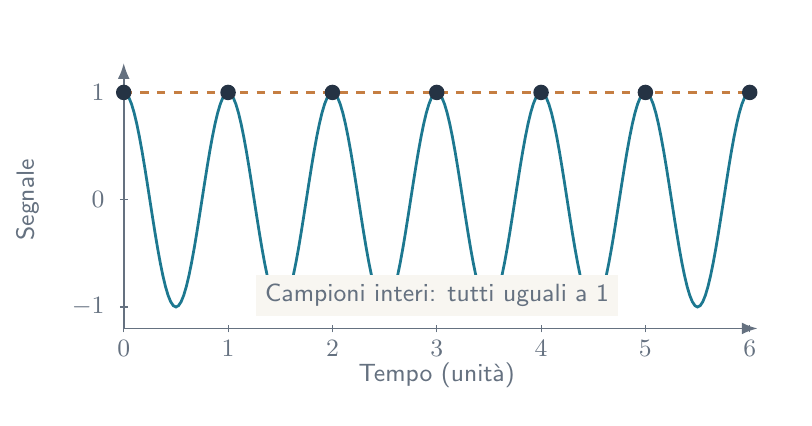
\begin{tikzpicture}[x=1cm,y=1cm]
\path[use as bounding box](-.3,-.2) rectangle(9.299999999999999,4.5);
\draw[pAxis](0.92,0.68)--(8.969999999999999,0.68);
\draw[pAxis](0.92,0.68)--(0.92,4.050000000000001);
\draw[Muted](0.9200,0.63)--(0.9200,0.7300000000000001);\node[pNote] at(0.9200,0.43000000000000005){$0$};
\draw[Muted](2.2450,0.63)--(2.2450,0.7300000000000001);\node[pNote] at(2.2450,0.43000000000000005){$1$};
\draw[Muted](3.5700,0.63)--(3.5700,0.7300000000000001);\node[pNote] at(3.5700,0.43000000000000005){$2$};
\draw[Muted](4.8950,0.63)--(4.8950,0.7300000000000001);\node[pNote] at(4.8950,0.43000000000000005){$3$};
\draw[Muted](6.2200,0.63)--(6.2200,0.7300000000000001);\node[pNote] at(6.2200,0.43000000000000005){$4$};
\draw[Muted](7.5450,0.63)--(7.5450,0.7300000000000001);\node[pNote] at(7.5450,0.43000000000000005){$5$};
\draw[Muted](8.8700,0.63)--(8.8700,0.7300000000000001);\node[pNote] at(8.8700,0.43000000000000005){$6$};
\draw[Muted](0.87,0.9525)--(0.9700000000000001,0.9525);\node[pNote,anchor=east] at(0.8,0.9525){$-1$};
\draw[Muted](0.87,2.3150)--(0.9700000000000001,2.3150);\node[pNote,anchor=east] at(0.8,2.3150){$0$};
\draw[Muted](0.87,3.6775)--(0.9700000000000001,3.6775);\node[pNote,anchor=east] at(0.8,3.6775){$1$};
\node[pNote] at(4.895,0.09000000000000008){Tempo (unità)};
\node[pNote,rotate=90] at(-.3,2.3150000000000004){Segnale};
\draw[GeoA,line width=1.0pt] plot coordinates {(0.9200,3.6775) (0.9531,3.6607) (0.9863,3.6108) (1.0194,3.5290) (1.0525,3.4173) (1.0856,3.2784) (1.1187,3.1159) (1.1519,2.9336) (1.1850,2.7360) (1.2181,2.5281) (1.2512,2.3150) (1.2844,2.1019) (1.3175,1.8940) (1.3506,1.6964) (1.3838,1.5141) (1.4169,1.3516) (1.4500,1.2127) (1.4831,1.1010) (1.5162,1.0192) (1.5494,0.9693) (1.5825,0.9525) (1.6156,0.9693) (1.6488,1.0192) (1.6819,1.1010) (1.7150,1.2127) (1.7481,1.3516) (1.7812,1.5141) (1.8144,1.6964) (1.8475,1.8940) (1.8806,2.1019) (1.9137,2.3150) (1.9469,2.5281) (1.9800,2.7360) (2.0131,2.9336) (2.0463,3.1159) (2.0794,3.2784) (2.1125,3.4173) (2.1456,3.5290) (2.1787,3.6108) (2.2119,3.6607) (2.2450,3.6775) (2.2781,3.6607) (2.3113,3.6108) (2.3444,3.5290) (2.3775,3.4173) (2.4106,3.2784) (2.4437,3.1159) (2.4769,2.9336) (2.5100,2.7360) (2.5431,2.5281) (2.5762,2.3150) (2.6094,2.1019) (2.6425,1.8940) (2.6756,1.6964) (2.7087,1.5141) (2.7419,1.3516) (2.7750,1.2127) (2.8081,1.1010) (2.8413,1.0192) (2.8744,0.9693) (2.9075,0.9525) (2.9406,0.9693) (2.9737,1.0192) (3.0069,1.1010) (3.0400,1.2127) (3.0731,1.3516) (3.1062,1.5141) (3.1394,1.6964) (3.1725,1.8940) (3.2056,2.1019) (3.2388,2.3150) (3.2719,2.5281) (3.3050,2.7360) (3.3381,2.9336) (3.3712,3.1159) (3.4044,3.2784) (3.4375,3.4173) (3.4706,3.5290) (3.5037,3.6108) (3.5369,3.6607) (3.5700,3.6775) (3.6031,3.6607) (3.6362,3.6108) (3.6694,3.5290) (3.7025,3.4173) (3.7356,3.2784) (3.7687,3.1159) (3.8019,2.9336) (3.8350,2.7360) (3.8681,2.5281) (3.9012,2.3150) (3.9344,2.1019) (3.9675,1.8940) (4.0006,1.6964) (4.0337,1.5141) (4.0669,1.3516) (4.1000,1.2127) (4.1331,1.1010) (4.1663,1.0192) (4.1994,0.9693) (4.2325,0.9525) (4.2656,0.9693) (4.2988,1.0192) (4.3319,1.1010) (4.3650,1.2127) (4.3981,1.3516) (4.4312,1.5141) (4.4644,1.6964) (4.4975,1.8940) (4.5306,2.1019) (4.5637,2.3150) (4.5969,2.5281) (4.6300,2.7360) (4.6631,2.9336) (4.6963,3.1159) (4.7294,3.2784) (4.7625,3.4173) (4.7956,3.5290) (4.8288,3.6108) (4.8619,3.6607) (4.8950,3.6775) (4.9281,3.6607) (4.9612,3.6108) (4.9944,3.5290) (5.0275,3.4173) (5.0606,3.2784) (5.0938,3.1159) (5.1269,2.9336) (5.1600,2.7360) (5.1931,2.5281) (5.2262,2.3150) (5.2594,2.1019) (5.2925,1.8940) (5.3256,1.6964) (5.3587,1.5141) (5.3919,1.3516) (5.4250,1.2127) (5.4581,1.1010) (5.4912,1.0192) (5.5244,0.9693) (5.5575,0.9525) (5.5906,0.9693) (5.6237,1.0192) (5.6569,1.1010) (5.6900,1.2127) (5.7231,1.3516) (5.7562,1.5141) (5.7894,1.6964) (5.8225,1.8940) (5.8556,2.1019) (5.8887,2.3150) (5.9219,2.5281) (5.9550,2.7360) (5.9881,2.9336) (6.0213,3.1159) (6.0544,3.2784) (6.0875,3.4173) (6.1206,3.5290) (6.1537,3.6108) (6.1869,3.6607) (6.2200,3.6775) (6.2531,3.6607) (6.2862,3.6108) (6.3194,3.5290) (6.3525,3.4173) (6.3856,3.2784) (6.4188,3.1159) (6.4519,2.9336) (6.4850,2.7360) (6.5181,2.5281) (6.5512,2.3150) (6.5844,2.1019) (6.6175,1.8940) (6.6506,1.6964) (6.6837,1.5141) (6.7169,1.3516) (6.7500,1.2127) (6.7831,1.1010) (6.8162,1.0192) (6.8494,0.9693) (6.8825,0.9525) (6.9156,0.9693) (6.9487,1.0192) (6.9819,1.1010) (7.0150,1.2127) (7.0481,1.3516) (7.0812,1.5141) (7.1144,1.6964) (7.1475,1.8940) (7.1806,2.1019) (7.2137,2.3150) (7.2469,2.5281) (7.2800,2.7360) (7.3131,2.9336) (7.3462,3.1159) (7.3794,3.2784) (7.4125,3.4173) (7.4456,3.5290) (7.4787,3.6108) (7.5119,3.6607) (7.5450,3.6775) (7.5781,3.6607) (7.6112,3.6108) (7.6444,3.5290) (7.6775,3.4173) (7.7106,3.2784) (7.7437,3.1159) (7.7769,2.9336) (7.8100,2.7360) (7.8431,2.5281) (7.8762,2.3150) (7.9094,2.1019) (7.9425,1.8940) (7.9756,1.6964) (8.0087,1.5141) (8.0419,1.3516) (8.0750,1.2127) (8.1081,1.1010) (8.1412,1.0192) (8.1744,0.9693) (8.2075,0.9525) (8.2406,0.9693) (8.2737,1.0192) (8.3069,1.1010) (8.3400,1.2127) (8.3731,1.3516) (8.4062,1.5141) (8.4394,1.6964) (8.4725,1.8940) (8.5056,2.1019) (8.5388,2.3150) (8.5719,2.5281) (8.6050,2.7360) (8.6381,2.9336) (8.6712,3.1159) (8.7044,3.2784) (8.7375,3.4173) (8.7706,3.5290) (8.8037,3.6108) (8.8369,3.6607) (8.8700,3.6775)};
\draw[GeoB,dashed,line width=1.2pt] plot coordinates {(0.9200,3.6775) (8.8700,3.6775)};
\fill[Ink](0.9200,3.6775)circle(2.8pt);
\fill[Ink](2.2450,3.6775)circle(2.8pt);
\fill[Ink](3.5700,3.6775)circle(2.8pt);
\fill[Ink](4.8950,3.6775)circle(2.8pt);
\fill[Ink](6.2200,3.6775)circle(2.8pt);
\fill[Ink](7.5450,3.6775)circle(2.8pt);
\fill[Ink](8.8700,3.6775)circle(2.8pt);
\node[pNote,fill=Paper] at(4.9,1.1){Campioni interi: tutti uguali a 1};
\end{tikzpicture}
\end{minipage}%
\end{lrbox}
\typeout{FULLBOX:023:L:\the\ht\PilotLeftBox:\the\dp\PilotLeftBox}
\begin{lrbox}{\PilotRightBox}%
\begin{minipage}[t]{7.55cm}\raggedright\color{Ink}\fontsize{11.3}{14.8}\selectfont
\PBody{Nel disegno, il segnale oscilla fra $-1$ e $1$. I campioni cadono sempre nella stessa fase e sono tutti uguali a 1.}
\vspace{3mm}
\[f_s>2f_{\max}.\]
\PSmall{Condizione del modello ideale: segnale limitato in frequenza e campionamento uniforme. $f_s$ è la frequenza di campionamento.}
\vspace{3mm}
\PInfo{L’aliasing rende indistinguibili frequenze diverse alla risoluzione osservata. Irregolarità e assenze richiedono analisi ulteriori.}
\end{minipage}%
\end{lrbox}
\typeout{FULLBOX:023:R:\the\ht\PilotRightBox:\the\dp\PilotRightBox}
\begin{tikzpicture}[remember picture,overlay]
\PilotChrome{Un campionamento rado può nascondere un ciclo}{II · AGGREGAZIONE E RISOLUZIONE}{23}{Una serie osservata quasi costante può derivare da un segnale variabile campionato sempre alla stessa fase.}
\node[anchor=north west,inner sep=0] at([xshift=0.96cm,yshift=-2.13cm]current page.north west){\usebox{\PilotLeftBox}};
\node[anchor=north west,inner sep=0] at([xshift=11.52cm,yshift=-2.13cm]current page.north west){\usebox{\PilotRightBox}};
\end{tikzpicture}\end{frame}

\begin{frame}[plain]\hypertarget{slide24}{}
\bookmark[level=1,page=24]{Risoluzione e copertura si esaminano insieme}
\begin{lrbox}{\PilotLeftBox}%
\begin{minipage}[t]{10.05cm}\raggedright\color{Ink}\fontsize{11.3}{14.8}\selectfont
\PLab{https://marzione00.github.io/Lab_Geo/\#laboratorio/m09-aggregazione}{Esperimento · Aggregazione}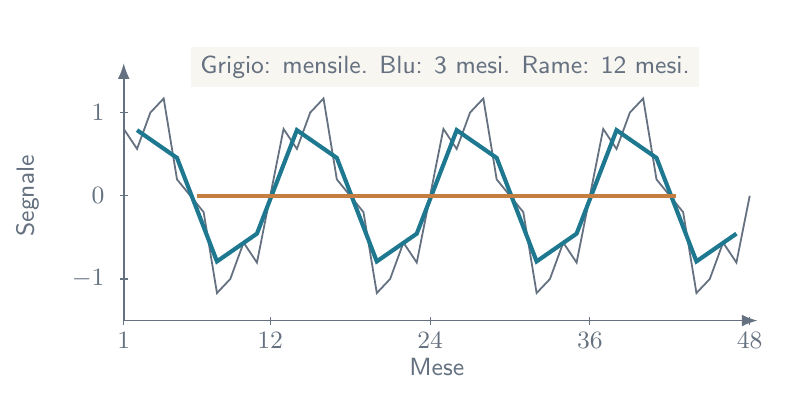
\begin{tikzpicture}[x=1cm,y=1cm]
\path[use as bounding box](-.3,-.2) rectangle(9.299999999999999,4.3999999999999995);
\draw[pAxis](0.92,0.68)--(8.969999999999999,0.68);
\draw[pAxis](0.92,0.68)--(0.92,3.95);
\draw[Muted](0.9200,0.63)--(0.9200,0.7300000000000001);\node[pNote] at(0.9200,0.43000000000000005){$1$};
\draw[Muted](2.7806,0.63)--(2.7806,0.7300000000000001);\node[pNote] at(2.7806,0.43000000000000005){$12$};
\draw[Muted](4.8104,0.63)--(4.8104,0.7300000000000001);\node[pNote] at(4.8104,0.43000000000000005){$24$};
\draw[Muted](6.8402,0.63)--(6.8402,0.7300000000000001);\node[pNote] at(6.8402,0.43000000000000005){$36$};
\draw[Muted](8.8700,0.63)--(8.8700,0.7300000000000001);\node[pNote] at(8.8700,0.43000000000000005){$48$};
\draw[Muted](0.87,1.2083)--(0.9700000000000001,1.2083);\node[pNote,anchor=east] at(0.8,1.2083){$-1$};
\draw[Muted](0.87,2.2650)--(0.9700000000000001,2.2650);\node[pNote,anchor=east] at(0.8,2.2650){$0$};
\draw[Muted](0.87,3.3217)--(0.9700000000000001,3.3217);\node[pNote,anchor=east] at(0.8,3.3217){$1$};
\node[pNote] at(4.895,0.09000000000000008){Mese};
\node[pNote,rotate=90] at(-.3,2.265){Segnale};
\draw[Muted,line width=.65pt] plot coordinates {(0.9200,3.1136) (1.0891,2.8598) (1.2583,3.3217) (1.4274,3.5004) (1.5966,2.4730) (1.7657,2.2650) (1.9349,2.0570) (2.1040,1.0296) (2.2732,1.2083) (2.4423,1.6702) (2.6115,1.4164) (2.7806,2.2650) (2.9498,3.1136) (3.1189,2.8598) (3.2881,3.3217) (3.4572,3.5004) (3.6264,2.4730) (3.7955,2.2650) (3.9647,2.0570) (4.1338,1.0296) (4.3030,1.2083) (4.4721,1.6702) (4.6413,1.4164) (4.8104,2.2650) (4.9796,3.1136) (5.1487,2.8598) (5.3179,3.3217) (5.4870,3.5004) (5.6562,2.4730) (5.8253,2.2650) (5.9945,2.0570) (6.1636,1.0296) (6.3328,1.2083) (6.5019,1.6702) (6.6711,1.4164) (6.8402,2.2650) (7.0094,3.1136) (7.1785,2.8598) (7.3477,3.3217) (7.5168,3.5004) (7.6860,2.4730) (7.8551,2.2650) (8.0243,2.0570) (8.1934,1.0296) (8.3626,1.2083) (8.5317,1.6702) (8.7009,1.4164) (8.8700,2.2650)};
\draw[GeoA,line width=1.5pt] plot coordinates {(1.0891,3.0984) (1.5966,2.7461) (2.1040,1.4316) (2.6115,1.7839) (3.1189,3.0984) (3.6264,2.7461) (4.1338,1.4316) (4.6413,1.7839) (5.1487,3.0984) (5.6562,2.7461) (6.1636,1.4316) (6.6711,1.7839) (7.1785,3.0984) (7.6860,2.7461) (8.1934,1.4316) (8.7009,1.7839)};
\draw[GeoB,line width=1.5pt] plot coordinates {(1.8503,2.2650) (3.8801,2.2650) (5.9099,2.2650) (7.9397,2.2650)};
\node[pNote,fill=Paper] at(5,3.9){Grigio: mensile. Blu: 3 mesi. Rame: 12 mesi.};
\end{tikzpicture}
\end{minipage}%
\end{lrbox}
\typeout{FULLBOX:024:L:\the\ht\PilotLeftBox:\the\dp\PilotLeftBox}
\begin{lrbox}{\PilotRightBox}%
\begin{minipage}[t]{7.55cm}\raggedright\color{Ink}\fontsize{11.3}{14.8}\selectfont
\PBody{Nell’esperimento, allargare l’intervallo di aggregazione modifica la forma e la variabilità della serie.}
\vspace{3mm}
\PInfo{Confrontare finestre da 1, 3 e 12 mesi. Descrivere quale oscillazione si attenua e quali picchi non restano riconoscibili.}
\vspace{3mm}
\PBody{Il confronto è interpretabile se teniamo ferma anche la regola sulle assenze. Un cambiamento di copertura può alterare la media quanto un cambiamento del segnale.}
\vspace{3mm}
\PSmall{\href{https://marzione00.github.io/Lab_Geo/\#laboratorio/m09-calendario}{Esperimento complementare: calendario e mesi mancanti}}
\end{minipage}%
\end{lrbox}
\typeout{FULLBOX:024:R:\the\ht\PilotRightBox:\the\dp\PilotRightBox}
\begin{tikzpicture}[remember picture,overlay]
\PilotChrome{Risoluzione e copertura si esaminano insieme}{II · AGGREGAZIONE E RISOLUZIONE}{24}{L’aggregazione modifica insieme il dettaglio visibile e il significato delle osservazioni.}
\node[anchor=north west,inner sep=0] at([xshift=0.96cm,yshift=-2.13cm]current page.north west){\usebox{\PilotLeftBox}};
\node[anchor=north west,inner sep=0] at([xshift=11.52cm,yshift=-2.13cm]current page.north west){\usebox{\PilotRightBox}};
\end{tikzpicture}\end{frame}

\begin{frame}[plain]\hypertarget{slide25}{}
\bookmark[level=1,page=25]{Il dato analizzabile conserva la sua storia}
\begin{lrbox}{\PilotLeftBox}%
\begin{minipage}[t]{10.05cm}\raggedright\color{Ink}\fontsize{11.3}{14.8}\selectfont
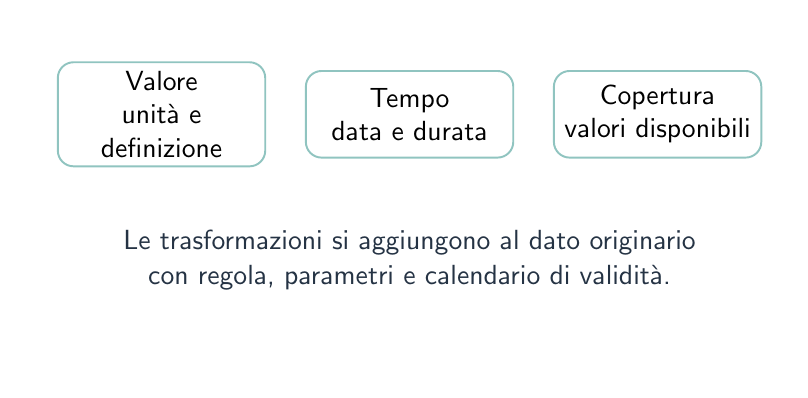
\begin{tikzpicture}[x=1cm,y=1cm]
\path[use as bounding box](-.15,-.15) rectangle(9.4,4.2);
\node[pFlow,text width=2.4cm] (a) at(1.55,3.1){Valore\\unità e definizione};\node[pFlow,text width=2.4cm] (b) at(4.7,3.1){Tempo\\data e durata};\node[pFlow,text width=2.4cm] (c) at(7.85,3.1){Copertura\\valori disponibili};\node[pLabel,text width=8.5cm] at(4.7,1.25){Le trasformazioni si aggiungono al dato originario\\con regola, parametri e calendario di validità.};
\end{tikzpicture}
\end{minipage}%
\end{lrbox}
\typeout{FULLBOX:025:L:\the\ht\PilotLeftBox:\the\dp\PilotLeftBox}
\begin{lrbox}{\PilotRightBox}%
\begin{minipage}[t]{7.55cm}\raggedright\color{Ink}\fontsize{11.3}{14.8}\selectfont
\PCode{R · preparare il registro}{025_registro.R}\PBody{Passiamo ora alla forma della serie: andamento graduale, oscillazione periodica e variazioni che restano dopo averle rappresentate.}
\end{minipage}%
\end{lrbox}
\typeout{FULLBOX:025:R:\the\ht\PilotRightBox:\the\dp\PilotRightBox}
\begin{tikzpicture}[remember picture,overlay]
\PilotChrome{Il dato analizzabile conserva la sua storia}{II · AGGREGAZIONE E RISOLUZIONE}{25}{Un’analisi riproducibile mantiene collegati osservazione originaria, calendario e trasformazioni.}
\node[anchor=north west,inner sep=0] at([xshift=0.96cm,yshift=-2.13cm]current page.north west){\usebox{\PilotLeftBox}};
\node[anchor=north west,inner sep=0] at([xshift=11.52cm,yshift=-2.13cm]current page.north west){\usebox{\PilotRightBox}};
\end{tikzpicture}\end{frame}

\begin{frame}[plain]\hypertarget{slide26}{}
\bookmark[level=0,page=26]{Trend, stagione e smoothing}
\bookmark[level=1,page=26]{Una serie può essere descritta per componenti}
\begin{lrbox}{\PilotLeftBox}%
\begin{minipage}[t]{10.05cm}\raggedright\color{Ink}\fontsize{11.3}{14.8}\selectfont
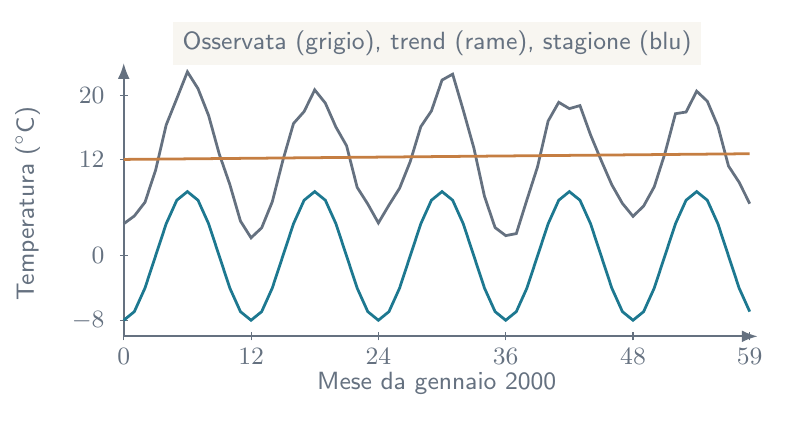
\begin{tikzpicture}[x=1cm,y=1cm]
\path[use as bounding box](-.3,-.2) rectangle(9.299999999999999,4.6);
\draw[pAxis](0.92,0.68)--(8.969999999999999,0.68);
\draw[pAxis](0.92,0.68)--(0.92,4.1499999999999995);
\draw[Muted](0.9200,0.63)--(0.9200,0.7300000000000001);\node[pNote] at(0.9200,0.43000000000000005){$0$};
\draw[Muted](2.5369,0.63)--(2.5369,0.7300000000000001);\node[pNote] at(2.5369,0.43000000000000005){$12$};
\draw[Muted](4.1539,0.63)--(4.1539,0.7300000000000001);\node[pNote] at(4.1539,0.43000000000000005){$24$};
\draw[Muted](5.7708,0.63)--(5.7708,0.7300000000000001);\node[pNote] at(5.7708,0.43000000000000005){$36$};
\draw[Muted](7.3878,0.63)--(7.3878,0.7300000000000001);\node[pNote] at(7.3878,0.43000000000000005){$48$};
\draw[Muted](8.8700,0.63)--(8.8700,0.7300000000000001);\node[pNote] at(8.8700,0.43000000000000005){$59$};
\draw[Muted](0.87,0.8842)--(0.9700000000000001,0.8842);\node[pNote,anchor=east] at(0.8,0.8842){$-8$};
\draw[Muted](0.87,1.7012)--(0.9700000000000001,1.7012);\node[pNote,anchor=east] at(0.8,1.7012){$0$};
\draw[Muted](0.87,2.9267)--(0.9700000000000001,2.9267);\node[pNote,anchor=east] at(0.8,2.9267){$12$};
\draw[Muted](0.87,3.7436)--(0.9700000000000001,3.7436);\node[pNote,anchor=east] at(0.8,3.7436){$20$};
\node[pNote] at(4.895,0.09000000000000008){Mese da gennaio 2000};
\node[pNote,rotate=90] at(-.3,2.365){Temperatura ($^\circ$C)};
\draw[Muted,line width=1.0pt] plot coordinates {(0.9200,2.1097) (1.0547,2.2086) (1.1895,2.3825) (1.3242,2.7879) (1.4590,3.3641) (1.5937,3.6993) (1.7285,4.0389) (1.8632,3.8260) (1.9980,3.4841) (2.1327,2.9964) (2.2675,2.6078) (2.4022,2.1444) (2.5369,1.9312) (2.6717,2.0580) (2.8064,2.3885) (2.9412,2.9158) (3.0759,3.3829) (3.2107,3.5348) (3.3454,3.8099) (3.4802,3.6422) (3.6149,3.3372) (3.7497,3.1009) (3.8844,2.5722) (4.0192,2.3606) (4.1539,2.1199) (4.2886,2.3466) (4.4234,2.5612) (4.5581,2.8982) (4.6929,3.3432) (4.8276,3.5425) (4.9624,3.9349) (5.0971,4.0095) (5.2319,3.5516) (5.3666,3.0718) (5.5014,2.4579) (5.6361,2.0611) (5.7708,1.9592) (5.9056,1.9846) (6.0403,2.4134) (6.1751,2.8328) (6.3098,3.4143) (6.4446,3.6520) (6.5793,3.5718) (6.7141,3.6102) (6.8488,3.2375) (6.9836,2.9136) (7.1183,2.6047) (7.2531,2.3683) (7.3878,2.2042) (7.5225,2.3347) (7.6573,2.5785) (7.7920,2.9995) (7.9268,3.5073) (8.0615,3.5288) (8.1963,3.7933) (8.3310,3.6658) (8.4658,3.3504) (8.6005,2.8431) (8.7353,2.6364) (8.8700,2.3647)};
\draw[GeoB,line width=1.0pt] plot coordinates {(0.9200,2.9267) (1.0547,2.9279) (1.1895,2.9291) (1.3242,2.9303) (1.4590,2.9316) (1.5937,2.9328) (1.7285,2.9340) (1.8632,2.9352) (1.9980,2.9365) (2.1327,2.9377) (2.2675,2.9389) (2.4022,2.9401) (2.5369,2.9414) (2.6717,2.9426) (2.8064,2.9438) (2.9412,2.9450) (3.0759,2.9463) (3.2107,2.9475) (3.3454,2.9487) (3.4802,2.9500) (3.6149,2.9512) (3.7497,2.9524) (3.8844,2.9536) (4.0192,2.9549) (4.1539,2.9561) (4.2886,2.9573) (4.4234,2.9585) (4.5581,2.9598) (4.6929,2.9610) (4.8276,2.9622) (4.9624,2.9634) (5.0971,2.9647) (5.2319,2.9659) (5.3666,2.9671) (5.5014,2.9683) (5.6361,2.9696) (5.7708,2.9708) (5.9056,2.9720) (6.0403,2.9732) (6.1751,2.9745) (6.3098,2.9757) (6.4446,2.9769) (6.5793,2.9781) (6.7141,2.9794) (6.8488,2.9806) (6.9836,2.9818) (7.1183,2.9830) (7.2531,2.9843) (7.3878,2.9855) (7.5225,2.9867) (7.6573,2.9879) (7.7920,2.9892) (7.9268,2.9904) (8.0615,2.9916) (8.1963,2.9928) (8.3310,2.9941) (8.4658,2.9953) (8.6005,2.9965) (8.7353,2.9977) (8.8700,2.9990)};
\draw[GeoA,line width=1.0pt] plot coordinates {(0.9200,0.8842) (1.0547,0.9937) (1.1895,1.2927) (1.3242,1.7012) (1.4590,2.1097) (1.5937,2.4087) (1.7285,2.5182) (1.8632,2.4087) (1.9980,2.1097) (2.1327,1.7012) (2.2675,1.2927) (2.4022,0.9937) (2.5369,0.8842) (2.6717,0.9937) (2.8064,1.2927) (2.9412,1.7012) (3.0759,2.1097) (3.2107,2.4087) (3.3454,2.5182) (3.4802,2.4087) (3.6149,2.1097) (3.7497,1.7012) (3.8844,1.2927) (4.0192,0.9937) (4.1539,0.8842) (4.2886,0.9937) (4.4234,1.2927) (4.5581,1.7012) (4.6929,2.1097) (4.8276,2.4087) (4.9624,2.5182) (5.0971,2.4087) (5.2319,2.1097) (5.3666,1.7012) (5.5014,1.2927) (5.6361,0.9937) (5.7708,0.8842) (5.9056,0.9937) (6.0403,1.2927) (6.1751,1.7012) (6.3098,2.1097) (6.4446,2.4087) (6.5793,2.5182) (6.7141,2.4087) (6.8488,2.1097) (6.9836,1.7012) (7.1183,1.2927) (7.2531,0.9937) (7.3878,0.8842) (7.5225,0.9937) (7.6573,1.2927) (7.7920,1.7012) (7.9268,2.1097) (8.0615,2.4087) (8.1963,2.5182) (8.3310,2.4087) (8.4658,2.1097) (8.6005,1.7012) (8.7353,1.2927) (8.8700,0.9937)};
\node[pNote,fill=Paper] at(4.9,4.4){Osservata (grigio), trend (rame), stagione (blu)};
\end{tikzpicture}\[X_t=T_t+S_t+R_t.\]
\end{minipage}%
\end{lrbox}
\typeout{FULLBOX:026:L:\the\ht\PilotLeftBox:\the\dp\PilotLeftBox}
\begin{lrbox}{\PilotRightBox}%
\begin{minipage}[t]{7.55cm}\raggedright\color{Ink}\fontsize{11.3}{14.8}\selectfont
\PBody{Un andamento graduale $T_t$ e una stagione $S_t$ descrivono due scale di variazione. Il resto $R_t$ raccoglie ciò che rimane dopo questa rappresentazione.}
\vspace{3mm}
\PInfo{Nella temperatura simulata conosciamo le componenti del generatore. Nei dati osservati dobbiamo stimarle attraverso un modello.}
\vspace{3mm}
\PBody{La scomposizione additiva è una scelta. Componenti con ampiezza proporzionale al livello possono richiedere una trasformazione, se compatibile con il significato e il dominio dei dati.}
\end{minipage}%
\end{lrbox}
\typeout{FULLBOX:026:R:\the\ht\PilotRightBox:\the\dp\PilotRightBox}
\begin{tikzpicture}[remember picture,overlay]
\PilotChrome{Una serie può essere descritta per componenti}{III · TREND, STAGIONE E SMOOTHING}{26}{Le componenti dipendono dalla rappresentazione adottata. Il resto può conservare struttura.}
\node[anchor=north west,inner sep=0] at([xshift=0.96cm,yshift=-2.13cm]current page.north west){\usebox{\PilotLeftBox}};
\node[anchor=north west,inner sep=0] at([xshift=11.52cm,yshift=-2.13cm]current page.north west){\usebox{\PilotRightBox}};
\end{tikzpicture}\end{frame}

\begin{frame}[plain]\hypertarget{slide27}{}
\bookmark[level=1,page=27]{Nel simulatore conosciamo le componenti}
\begin{lrbox}{\PilotLeftBox}%
\begin{minipage}[t]{10.05cm}\raggedright\color{Ink}\fontsize{11.3}{14.8}\selectfont
\begin{tikzpicture}[x=1cm,y=1cm]
\path[use as bounding box](-.3,-.2) rectangle(9.299999999999999,4.199999999999999);
\draw[pAxis](0.92,0.68)--(8.969999999999999,0.68);
\draw[pAxis](0.92,0.68)--(0.92,3.75);
\draw[Muted](0.9200,0.63)--(0.9200,0.7300000000000001);\node[pNote] at(0.9200,0.43000000000000005){$0$};
\draw[Muted](4.8950,0.63)--(4.8950,0.7300000000000001);\node[pNote] at(4.8950,0.43000000000000005){$29{,}5$};
\draw[Muted](8.8700,0.63)--(8.8700,0.7300000000000001);\node[pNote] at(8.8700,0.43000000000000005){$59$};
\draw[Muted](0.87,0.9065)--(0.9700000000000001,0.9065);\node[pNote,anchor=east] at(0.8,0.9065){$-8$};
\draw[Muted](0.87,3.4235)--(0.9700000000000001,3.4235);\node[pNote,anchor=east] at(0.8,3.4235){$12{,}708$};
\node[pNote] at(4.895,0.09000000000000008){Mese da gennaio 2000};
\node[pNote,rotate=90] at(-.3,2.165){$^\circ$C};
\draw[GeoA,line width=1.0pt] plot coordinates {(0.9200,3.3374) (1.0547,3.3389) (1.1895,3.3403) (1.3242,3.3418) (1.4590,3.3433) (1.5937,3.3447) (1.7285,3.3462) (1.8632,3.3476) (1.9980,3.3491) (2.1327,3.3505) (2.2675,3.3520) (2.4022,3.3535) (2.5369,3.3549) (2.6717,3.3564) (2.8064,3.3578) (2.9412,3.3593) (3.0759,3.3608) (3.2107,3.3622) (3.3454,3.3637) (3.4802,3.3651) (3.6149,3.3666) (3.7497,3.3681) (3.8844,3.3695) (4.0192,3.3710) (4.1539,3.3724) (4.2886,3.3739) (4.4234,3.3753) (4.5581,3.3768) (4.6929,3.3783) (4.8276,3.3797) (4.9624,3.3812) (5.0971,3.3826) (5.2319,3.3841) (5.3666,3.3856) (5.5014,3.3870) (5.6361,3.3885) (5.7708,3.3899) (5.9056,3.3914) (6.0403,3.3928) (6.1751,3.3943) (6.3098,3.3958) (6.4446,3.3972) (6.5793,3.3987) (6.7141,3.4001) (6.8488,3.4016) (6.9836,3.4031) (7.1183,3.4045) (7.2531,3.4060) (7.3878,3.4074) (7.5225,3.4089) (7.6573,3.4103) (7.7920,3.4118) (7.9268,3.4133) (8.0615,3.4147) (8.1963,3.4162) (8.3310,3.4176) (8.4658,3.4191) (8.6005,3.4206) (8.7353,3.4220) (8.8700,3.4235)};
\draw[GeoB,line width=1.0pt] plot coordinates {(0.9200,0.9065) (1.0547,1.0368) (1.1895,1.3927) (1.3242,1.8789) (1.4590,2.3651) (1.5937,2.7210) (1.7285,2.8512) (1.8632,2.7210) (1.9980,2.3651) (2.1327,1.8789) (2.2675,1.3927) (2.4022,1.0368) (2.5369,0.9065) (2.6717,1.0368) (2.8064,1.3927) (2.9412,1.8789) (3.0759,2.3651) (3.2107,2.7210) (3.3454,2.8512) (3.4802,2.7210) (3.6149,2.3651) (3.7497,1.8789) (3.8844,1.3927) (4.0192,1.0368) (4.1539,0.9065) (4.2886,1.0368) (4.4234,1.3927) (4.5581,1.8789) (4.6929,2.3651) (4.8276,2.7210) (4.9624,2.8512) (5.0971,2.7210) (5.2319,2.3651) (5.3666,1.8789) (5.5014,1.3927) (5.6361,1.0368) (5.7708,0.9065) (5.9056,1.0368) (6.0403,1.3927) (6.1751,1.8789) (6.3098,2.3651) (6.4446,2.7210) (6.5793,2.8512) (6.7141,2.7210) (6.8488,2.3651) (6.9836,1.8789) (7.1183,1.3927) (7.2531,1.0368) (7.3878,0.9065) (7.5225,1.0368) (7.6573,1.3927) (7.7920,1.8789) (7.9268,2.3651) (8.0615,2.7210) (8.1963,2.8512) (8.3310,2.7210) (8.4658,2.3651) (8.6005,1.8789) (8.7353,1.3927) (8.8700,1.0368)};
\end{tikzpicture}\PSmall{Trend in blu, stagione in rame. Le due curve hanno la stessa unità.}\PBody{L’identità consente di confrontare una stima delle componenti con la verità del simulatore.}
\end{minipage}%
\end{lrbox}
\typeout{FULLBOX:027:L:\the\ht\PilotLeftBox:\the\dp\PilotLeftBox}
\begin{lrbox}{\PilotRightBox}%
\begin{minipage}[t]{7.55cm}\raggedright\color{Ink}\fontsize{11.3}{14.8}\selectfont
\[T_t=12+0{,}012t,\qquad S_t=-8\cos\!\left(\frac{2\pi t}{12}\right).\]
\PSmall{$t=0$ corrisponde a gennaio 2000. Il file comprende 240 mesi.}\PCode{R · verificare l’identità}{027_componenti.R}
\end{minipage}%
\end{lrbox}
\typeout{FULLBOX:027:R:\the\ht\PilotRightBox:\the\dp\PilotRightBox}
\begin{tikzpicture}[remember picture,overlay]
\PilotChrome{Nel simulatore conosciamo le componenti}{III · TREND, STAGIONE E SMOOTHING}{27}{Conoscere il generatore permette di distinguere una ricostruzione esatta da una stima statistica.}
\node[anchor=north west,inner sep=0] at([xshift=0.96cm,yshift=-2.13cm]current page.north west){\usebox{\PilotLeftBox}};
\node[anchor=north west,inner sep=0] at([xshift=11.52cm,yshift=-2.13cm]current page.north west){\usebox{\PilotRightBox}};
\end{tikzpicture}\end{frame}

\begin{frame}[plain]\hypertarget{slide28}{}
\bookmark[level=1,page=28]{La stagione ricorre entro l’anno}
\begin{lrbox}{\PilotLeftBox}%
\begin{minipage}[t]{10.05cm}\raggedright\color{Ink}\fontsize{11.3}{14.8}\selectfont
\begin{tikzpicture}[x=1cm,y=1cm]
\path[use as bounding box](-.3,-.2) rectangle(9.299999999999999,4.5);
\draw[pAxis](0.92,0.68)--(8.969999999999999,0.68);
\draw[pAxis](0.92,0.68)--(0.92,4.050000000000001);
\draw[Muted](0.9200,0.63)--(0.9200,0.7300000000000001);\node[pNote] at(0.9200,0.43000000000000005){$1$};
\draw[Muted](3.0882,0.63)--(3.0882,0.7300000000000001);\node[pNote] at(3.0882,0.43000000000000005){$4$};
\draw[Muted](5.2564,0.63)--(5.2564,0.7300000000000001);\node[pNote] at(5.2564,0.43000000000000005){$7$};
\draw[Muted](7.4245,0.63)--(7.4245,0.7300000000000001);\node[pNote] at(7.4245,0.43000000000000005){$10$};
\draw[Muted](8.8700,0.63)--(8.8700,0.7300000000000001);\node[pNote] at(8.8700,0.43000000000000005){$12$};
\draw[Muted](0.87,0.6800)--(0.9700000000000001,0.6800);\node[pNote,anchor=east] at(0.8,0.6800){$340$};
\draw[Muted](0.87,1.6143)--(0.9700000000000001,1.6143);\node[pNote,anchor=east] at(0.8,1.6143){$350$};
\draw[Muted](0.87,2.5486)--(0.9700000000000001,2.5486);\node[pNote,anchor=east] at(0.8,2.5486){$360$};
\draw[Muted](0.87,3.4829)--(0.9700000000000001,3.4829);\node[pNote,anchor=east] at(0.8,3.4829){$370$};
\node[pNote] at(4.895,0.09000000000000008){Mese};
\node[pNote,rotate=90] at(-.3,2.3150000000000004){CO$_2$ (ppm)};
\draw[GeoA,line width=1.0pt] plot coordinates {(0.9200,1.1401) (1.6427,1.2289) (2.3655,1.3751) (3.0882,1.4578) (3.8109,1.5045) (4.5336,1.4442) (5.2564,1.2826) (5.9791,1.0817) (6.7018,0.9603) (7.4245,0.9416) (8.1473,1.0743) (8.8700,1.2009)};
\draw[GeoB,line width=1.0pt] plot coordinates {(0.9200,2.1655) (1.6427,2.2384) (2.3655,2.3524) (3.0882,2.4621) (3.8109,2.5056) (4.5336,2.4668) (5.2564,2.2683) (5.9791,2.0683) (6.7018,1.8969) (7.4245,1.9338) (8.1473,2.0067) (8.8700,2.1141)};
\draw[GeoC,line width=1.0pt] plot coordinates {(0.9200,3.4992) (1.6427,3.6066) (2.3655,3.6753) (3.0882,3.7421) (3.8109,3.8379) (4.5336,3.7687) (5.2564,3.6043) (5.9791,3.4291) (6.7018,3.2848) (7.4245,3.3007) (8.1473,3.4245) (8.8700,3.5782)};
\node[pNote,fill=Paper] at(4.9,4.05){1985: blu. 1992: rame. 2001: viola.};
\end{tikzpicture}
\end{minipage}%
\end{lrbox}
\typeout{FULLBOX:028:L:\the\ht\PilotLeftBox:\the\dp\PilotLeftBox}
\begin{lrbox}{\PilotRightBox}%
\begin{minipage}[t]{7.55cm}\raggedright\color{Ink}\fontsize{11.3}{14.8}\selectfont
\PCode{R · confrontare gli anni}{028_stagione.R}\PBody{La forma entro l’anno può ripetersi mentre il livello cresce. Un ciclo di calendario si distingue da oscillazioni con durata variabile.}
\end{minipage}%
\end{lrbox}
\typeout{FULLBOX:028:R:\the\ht\PilotRightBox:\the\dp\PilotRightBox}
\begin{tikzpicture}[remember picture,overlay]
\PilotChrome{La stagione ricorre entro l’anno}{III · TREND, STAGIONE E SMOOTHING}{28}{Il confronto fra gli stessi mesi di anni diversi aiuta a riconoscere la stagionalità.}
\node[anchor=north west,inner sep=0] at([xshift=0.96cm,yshift=-2.13cm]current page.north west){\usebox{\PilotLeftBox}};
\node[anchor=north west,inner sep=0] at([xshift=11.52cm,yshift=-2.13cm]current page.north west){\usebox{\PilotRightBox}};
\end{tikzpicture}\end{frame}

\begin{frame}[plain]\hypertarget{slide29}{}
\bookmark[level=1,page=29]{Una media mobile combina valori vicini}
\begin{lrbox}{\PilotLeftBox}%
\begin{minipage}[t]{10.05cm}\raggedright\color{Ink}\fontsize{11.3}{14.8}\selectfont
\begin{tikzpicture}[x=1cm,y=1cm]
\path[use as bounding box](-.15,-.15) rectangle(9.4,4.4);
\fill[GeoA](0.6,2.05)circle(3pt);\node[pNote] at(0.6,1){$t-4$};\fill[GeoA](1.63,2.05)circle(3pt);\node[pNote] at(1.63,1){$t-3$};\fill[GeoA!13](2.23,1.3)rectangle(3.0900000000000003,3.1);\fill[GeoA](2.66,2.05)circle(3pt);\node[pNote] at(2.66,1){$t-2$};\node[pNote] at(2.66,2.65){$1/5$};\fill[GeoA!13](3.26,1.3)rectangle(4.12,3.1);\fill[GeoA](3.69,2.05)circle(3pt);\node[pNote] at(3.69,1){$t-1$};\node[pNote] at(3.69,2.65){$1/5$};\fill[GeoA!13](4.29,1.3)rectangle(5.1499999999999995,3.1);\fill[GeoA](4.72,2.05)circle(3pt);\node[pNote] at(4.72,1){$t$};\node[pNote] at(4.72,2.65){$1/5$};\fill[GeoB!13](5.32,1.3)rectangle(6.18,3.1);\fill[GeoB](5.75,2.05)circle(3pt);\node[pNote] at(5.75,1){$t+1$};\node[pNote] at(5.75,2.65){$1/5$};\fill[GeoB!13](6.35,1.3)rectangle(7.209999999999999,3.1);\fill[GeoB](6.779999999999999,2.05)circle(3pt);\node[pNote] at(6.779999999999999,1){$t+2$};\node[pNote] at(6.779999999999999,2.65){$1/5$};\fill[GeoB](7.81,2.05)circle(3pt);\node[pNote] at(7.81,1){$t+3$};\fill[GeoB](8.84,2.05)circle(3pt);\node[pNote] at(8.84,1){$t+4$};\draw[Ink,dashed](4.72,.6)--(4.72,3.5);\node[pLabel] at(4.7,4){Due valori sono successivi a $t$};
\end{tikzpicture}\[M_t^{(q)}=\frac{1}{2q+1}\sum_{j=-q}^{q}X_{t+j}.\]
\end{minipage}%
\end{lrbox}
\typeout{FULLBOX:029:L:\the\ht\PilotLeftBox:\the\dp\PilotLeftBox}
\begin{lrbox}{\PilotRightBox}%
\begin{minipage}[t]{7.55cm}\raggedright\color{Ink}\fontsize{11.3}{14.8}\selectfont
\PBody{La semilarghezza $q$ conta i vicini su ciascun lato. Con $q=2$ la finestra contiene cinque valori, tutti con peso $1/5$.}
\vspace{3mm}
\PInfo{Il risultato viene collocato al tempo centrale $t$. Un’oscillazione può attenuarsi quando la finestra include fasi diverse del ciclo.}
\vspace{3mm}
\PBody{La media mobile modifica la risoluzione con cui leggiamo l’andamento locale. La scelta della finestra va motivata rispetto alla domanda.}
\end{minipage}%
\end{lrbox}
\typeout{FULLBOX:029:R:\the\ht\PilotRightBox:\the\dp\PilotRightBox}
\begin{tikzpicture}[remember picture,overlay]
\PilotChrome{Una media mobile combina valori vicini}{III · TREND, STAGIONE E SMOOTHING}{29}{La larghezza della finestra stabilisce quali variazioni contribuiscono a ciascun valore smussato.}
\node[anchor=north west,inner sep=0] at([xshift=0.96cm,yshift=-2.13cm]current page.north west){\usebox{\PilotLeftBox}};
\node[anchor=north west,inner sep=0] at([xshift=11.52cm,yshift=-2.13cm]current page.north west){\usebox{\PilotRightBox}};
\end{tikzpicture}\end{frame}

\begin{frame}[plain]\hypertarget{slide30}{}
\bookmark[level=1,page=30]{Tre e tredici mesi mostrano dettagli diversi}
\begin{lrbox}{\PilotLeftBox}%
\begin{minipage}[t]{10.05cm}\raggedright\color{Ink}\fontsize{11.3}{14.8}\selectfont
\begin{tikzpicture}[x=1cm,y=1cm]
\path[use as bounding box](-.3,-.2) rectangle(9.299999999999999,4.3999999999999995);
\draw[pAxis](0.92,0.68)--(8.969999999999999,0.68);
\draw[pAxis](0.92,0.68)--(0.92,3.95);
\draw[Muted](0.9200,0.63)--(0.9200,0.7300000000000001);\node[pNote] at(0.9200,0.43000000000000005){$0$};
\draw[Muted](4.8950,0.63)--(4.8950,0.7300000000000001);\node[pNote] at(4.8950,0.43000000000000005){$35{,}5$};
\draw[Muted](8.8700,0.63)--(8.8700,0.7300000000000001);\node[pNote] at(8.8700,0.43000000000000005){$71$};
\draw[Muted](0.87,0.9218)--(0.9700000000000001,0.9218);\node[pNote,anchor=east] at(0.8,0.9218){$2{,}2524$};
\draw[Muted](0.87,3.6082)--(0.9700000000000001,3.6082);\node[pNote,anchor=east] at(0.8,3.6082){$22{,}892$};
\node[pNote] at(4.895,0.09000000000000008){Mese da gennaio 2000};
\node[pNote,rotate=90] at(-.3,2.265){Temperatura ($^\circ$C)};
\draw[GeoA,line width=1.0pt] plot coordinates {(0.9200,1.1492) (1.0320,1.2753) (1.1439,1.4970) (1.2559,2.0137) (1.3679,2.7481) (1.4799,3.1754) (1.5918,3.6082) (1.7038,3.3368) (1.8158,2.9010) (1.9277,2.2794) (2.0397,1.7842) (2.1517,1.1935) (2.2637,0.9218) (2.3756,1.0834) (2.4876,1.5046) (2.5996,2.1767) (2.7115,2.7720) (2.8235,2.9656) (2.9355,3.3163) (3.0475,3.1025) (3.1594,2.7138) (3.2714,2.4126) (3.3834,1.7387) (3.4954,1.4690) (3.6073,1.1622) (3.7193,1.4512) (3.8313,1.7247) (3.9432,2.1543) (4.0552,2.7214) (4.1672,2.9755) (4.2792,3.4756) (4.3911,3.5707) (4.5031,2.9870) (4.6151,2.3755) (4.7270,1.5930) (4.8390,1.0873) (4.9510,0.9574) (5.0630,0.9898) (5.1749,1.5363) (5.2869,2.0709) (5.3989,2.8121) (5.5108,3.1150) (5.6228,3.0129) (5.7348,3.0617) (5.8468,2.5867) (5.9587,2.1739) (6.0707,1.7802) (6.1827,1.4788) (6.2946,1.2697) (6.4066,1.4360) (6.5186,1.7468) (6.6306,2.2834) (6.7425,2.9306) (6.8545,2.9580) (6.9665,3.2951) (7.0785,3.1326) (7.1904,2.7306) (7.3024,2.0841) (7.4144,1.8206) (7.5263,1.4742) (7.6383,1.1957) (7.7503,1.4250) (7.8623,1.7447) (7.9742,2.2039) (8.0862,2.8800) (8.1982,3.0917) (8.3101,3.5000) (8.4221,3.2376) (8.5341,2.6389) (8.6461,2.0575) (8.7580,1.5930) (8.8700,1.3558)};
\draw[GeoB,line width=1.0pt] plot coordinates {(1.0320,1.3072) (1.1439,1.5953) (1.2559,2.0863) (1.3679,2.6457) (1.4799,3.1772) (1.5918,3.3735) (1.7038,3.2820) (1.8158,2.8391) (1.9277,2.3215) (2.0397,1.7523) (2.1517,1.2998) (2.2637,1.0662) (2.3756,1.1699) (2.4876,1.5882) (2.5996,2.1511) (2.7115,2.6381) (2.8235,3.0180) (2.9355,3.1281) (3.0475,3.0442) (3.1594,2.7430) (3.2714,2.2884) (3.3834,1.8734) (3.4954,1.4567) (3.6073,1.3608) (3.7193,1.4460) (3.8313,1.7767) (3.9432,2.2001) (4.0552,2.6171) (4.1672,3.0575) (4.2792,3.3406) (4.3911,3.3444) (4.5031,2.9778) (4.6151,2.3185) (4.7270,1.6853) (4.8390,1.2126) (4.9510,1.0115) (5.0630,1.1612) (5.1749,1.5323) (5.2869,2.1398) (5.3989,2.6660) (5.5108,2.9800) (5.6228,3.0632) (5.7348,2.8871) (5.8468,2.6075) (5.9587,2.1803) (6.0707,1.8110) (6.1827,1.5096) (6.2946,1.3949) (6.4066,1.4842) (6.5186,1.8221) (6.6306,2.3203) (6.7425,2.7240) (6.8545,3.0612) (6.9665,3.1285) (7.0785,3.0528) (7.1904,2.6491) (7.3024,2.2118) (7.4144,1.7930) (7.5263,1.4969) (7.6383,1.3650) (7.7503,1.4551) (7.8623,1.7912) (7.9742,2.2762) (8.0862,2.7252) (8.1982,3.1572) (8.3101,3.2764) (8.4221,3.1255) (8.5341,2.6447) (8.6461,2.0965) (8.7580,1.6688) (8.8700,1.3851)};
\draw[GeoC,line width=1.0pt] plot coordinates {(1.5918,2.1449) (1.7038,2.1398) (1.8158,2.1575) (1.9277,2.2097) (2.0397,2.2681) (2.1517,2.2848) (2.2637,2.2956) (2.3756,2.2567) (2.4876,2.2088) (2.5996,2.1713) (2.7115,2.1297) (2.8235,2.1054) (2.9355,2.1030) (3.0475,2.1437) (3.1594,2.1931) (3.2714,2.2431) (3.3834,2.2850) (3.4954,2.3006) (3.6073,2.3398) (3.7193,2.3594) (3.8313,2.3505) (3.9432,2.3245) (4.0552,2.2615) (4.1672,2.2113) (4.2792,2.1720) (4.3911,2.1587) (4.5031,2.1653) (4.6151,2.1919) (4.7270,2.2425) (4.8390,2.2728) (4.9510,2.2757) (5.0630,2.2438) (5.1749,2.1681) (5.2869,2.1056) (5.3989,2.0598) (5.5108,2.0510) (5.6228,2.0650) (5.7348,2.1019) (5.8468,2.1601) (5.9587,2.2176) (6.0707,2.2837) (6.1827,2.2949) (6.2946,2.3088) (6.4066,2.3180) (6.5186,2.2925) (6.6306,2.2538) (6.7425,2.2267) (6.8545,2.2031) (6.9665,2.1813) (7.0785,2.1933) (7.1904,2.2170) (7.3024,2.2522) (7.4144,2.2981) (7.5263,2.3105) (7.6383,2.3522) (7.7503,2.3477) (7.8623,2.3098) (7.9742,2.2580) (8.0862,2.2202) (8.1982,2.1845) (8.3101,2.1639) (8.4221,2.1716) (8.5341,2.2198) (8.6461,2.2631) (8.7580,2.3016) (8.8700,2.3229)};
\end{tikzpicture}\PSmall{Blu: osservata. Rame: media a 3 mesi. Viola: media a 13 mesi.}
\end{minipage}%
\end{lrbox}
\typeout{FULLBOX:030:L:\the\ht\PilotLeftBox:\the\dp\PilotLeftBox}
\begin{lrbox}{\PilotRightBox}%
\begin{minipage}[t]{7.55cm}\raggedright\color{Ink}\fontsize{11.3}{14.8}\selectfont
\PCode{R · confrontare due finestre}{030_media_mobile.R}\PInfo{La finestra di tredici mesi attenua fortemente il ciclo annuale. Non garantisce di eliminarlo esattamente: i pesi e il numero di mesi contano.}
\end{minipage}%
\end{lrbox}
\typeout{FULLBOX:030:R:\the\ht\PilotRightBox:\the\dp\PilotRightBox}
\begin{tikzpicture}[remember picture,overlay]
\PilotChrome{Tre e tredici mesi mostrano dettagli diversi}{III · TREND, STAGIONE E SMOOTHING}{30}{Una curva più liscia conserva meno dettaglio. La finestra deve essere sempre dichiarata.}
\node[anchor=north west,inner sep=0] at([xshift=0.96cm,yshift=-2.13cm]current page.north west){\usebox{\PilotLeftBox}};
\node[anchor=north west,inner sep=0] at([xshift=11.52cm,yshift=-2.13cm]current page.north west){\usebox{\PilotRightBox}};
\end{tikzpicture}\end{frame}

\begin{frame}[plain]\hypertarget{slide31}{}
\bookmark[level=1,page=31]{Ai bordi mancano alcuni vicini}
\begin{lrbox}{\PilotLeftBox}%
\begin{minipage}[t]{10.05cm}\raggedright\color{Ink}\fontsize{11.3}{14.8}\selectfont
\begin{tikzpicture}[x=1cm,y=1cm]
\path[use as bounding box](-.15,-.15) rectangle(9.4,4.1);
\filldraw[fill=Paper,draw=GeoB,dashed](0.25,1.6)rectangle(1.05,2.6);\node[pNote] at(0.65,2.1){?};\filldraw[fill=Paper,draw=GeoB,dashed](1.25,1.6)rectangle(2.05,2.6);\node[pNote] at(1.65,2.1){?};\filldraw[fill=GeoA!15,draw=GeoA,dashed](2.25,1.6)rectangle(3.05,2.6);\node[pNote] at(2.65,2.1){1};\filldraw[fill=GeoA!15,draw=GeoA,dashed](3.25,1.6)rectangle(4.05,2.6);\node[pNote] at(3.65,2.1){2};\filldraw[fill=GeoA!15,draw=GeoA,dashed](4.25,1.6)rectangle(5.050000000000001,2.6);\node[pNote] at(4.65,2.1){3};\filldraw[fill=GeoA!15,draw=GeoA,dashed](5.25,1.6)rectangle(6.050000000000001,2.6);\node[pNote] at(5.65,2.1){4};\filldraw[fill=GeoA!15,draw=GeoA,dashed](6.25,1.6)rectangle(7.050000000000001,2.6);\node[pNote] at(6.65,2.1){5};\filldraw[fill=GeoA!15,draw=GeoA,dashed](7.25,1.6)rectangle(8.05,2.6);\node[pNote] at(7.65,2.1){6};\filldraw[fill=GeoA!15,draw=GeoA,dashed](8.25,1.6)rectangle(9.05,2.6);\node[pNote] at(8.65,2.1){7};\draw[GeoB,line width=1.1pt,rounded corners=1mm](.2,1.4)rectangle(5.1,2.8);\node[pLabel] at(4.6,3.5){Finestra centrata sul primo valore};\node[pNote] at(4.5,.8){Due vicini precedenti sono fuori dall’archivio};
\end{tikzpicture}\PBody{Con una finestra centrata di $2q+1$ valori, i primi e gli ultimi $q$ risultati sono NA se non estendiamo la serie.}
\end{minipage}%
\end{lrbox}
\typeout{FULLBOX:031:L:\the\ht\PilotLeftBox:\the\dp\PilotLeftBox}
\begin{lrbox}{\PilotRightBox}%
\begin{minipage}[t]{7.55cm}\raggedright\color{Ink}\fontsize{11.3}{14.8}\selectfont
\PCode{R · riconoscere i bordi incompleti}{031_bordi.R}\PInfo{Una finestra più corta al bordo cambia la definizione della stima. Un’estensione artificiale introduce ipotesi sui dati esterni.}
\end{minipage}%
\end{lrbox}
\typeout{FULLBOX:031:R:\the\ht\PilotRightBox:\the\dp\PilotRightBox}
\begin{tikzpicture}[remember picture,overlay]
\PilotChrome{Ai bordi mancano alcuni vicini}{III · TREND, STAGIONE E SMOOTHING}{31}{La regola ai bordi è parte del metodo e può influenzare le conclusioni sulle osservazioni più recenti.}
\node[anchor=north west,inner sep=0] at([xshift=0.96cm,yshift=-2.13cm]current page.north west){\usebox{\PilotLeftBox}};
\node[anchor=north west,inner sep=0] at([xshift=11.52cm,yshift=-2.13cm]current page.north west){\usebox{\PilotRightBox}};
\end{tikzpicture}\end{frame}

\begin{frame}[plain]\hypertarget{slide32}{}
\bookmark[level=1,page=32]{Una finestra rivolta al passato è causale}
\begin{lrbox}{\PilotLeftBox}%
\begin{minipage}[t]{10.05cm}\raggedright\color{Ink}\fontsize{11.3}{14.8}\selectfont
\begin{tikzpicture}[x=1cm,y=1cm]
\path[use as bounding box](-.15,-.15) rectangle(9.4,4.4);
\fill[GeoA!13](0.16999999999999998,1.3)rectangle(1.03,3.1);\fill[GeoA](0.6,2.05)circle(3pt);\node[pNote] at(0.6,1){$t-4$};\node[pNote] at(0.6,2.65){$1/5$};\fill[GeoA!13](1.2,1.3)rectangle(2.06,3.1);\fill[GeoA](1.63,2.05)circle(3pt);\node[pNote] at(1.63,1){$t-3$};\node[pNote] at(1.63,2.65){$1/5$};\fill[GeoA!13](2.23,1.3)rectangle(3.0900000000000003,3.1);\fill[GeoA](2.66,2.05)circle(3pt);\node[pNote] at(2.66,1){$t-2$};\node[pNote] at(2.66,2.65){$1/5$};\fill[GeoA!13](3.26,1.3)rectangle(4.12,3.1);\fill[GeoA](3.69,2.05)circle(3pt);\node[pNote] at(3.69,1){$t-1$};\node[pNote] at(3.69,2.65){$1/5$};\fill[GeoA!13](4.29,1.3)rectangle(5.1499999999999995,3.1);\fill[GeoA](4.72,2.05)circle(3pt);\node[pNote] at(4.72,1){$t$};\node[pNote] at(4.72,2.65){$1/5$};\fill[GeoB](5.75,2.05)circle(3pt);\node[pNote] at(5.75,1){$t+1$};\fill[GeoB](6.779999999999999,2.05)circle(3pt);\node[pNote] at(6.779999999999999,1){$t+2$};\fill[GeoB](7.81,2.05)circle(3pt);\node[pNote] at(7.81,1){$t+3$};\fill[GeoB](8.84,2.05)circle(3pt);\node[pNote] at(8.84,1){$t+4$};\draw[Ink,dashed](4.72,.6)--(4.72,3.5);\node[pLabel] at(4.7,4){Cinque valori già disponibili};
\end{tikzpicture}\[M_t^-=\frac{1}{L}\sum_{j=0}^{L-1}X_{t-j}.\]
\end{minipage}%
\end{lrbox}
\typeout{FULLBOX:032:L:\the\ht\PilotLeftBox:\the\dp\PilotLeftBox}
\begin{lrbox}{\PilotRightBox}%
\begin{minipage}[t]{7.55cm}\raggedright\color{Ink}\fontsize{11.3}{14.8}\selectfont
\PCode{R · usare soltanto dati già disponibili}{032_filtro_causale.R}\PBody{$L$ indica il numero complessivo di valori, incluso il presente. Qui la finestra è causale nel senso temporale del filtro.}\vspace{3mm}\PInfo{La curva segue più lentamente un cambiamento. Questo ritardo è distinto dalla disponibilità di dati futuri.}
\end{minipage}%
\end{lrbox}
\typeout{FULLBOX:032:R:\the\ht\PilotRightBox:\the\dp\PilotRightBox}
\begin{tikzpicture}[remember picture,overlay]
\PilotChrome{Una finestra rivolta al passato è causale}{III · TREND, STAGIONE E SMOOTHING}{32}{Un filtro causale rispetta l’ordine di disponibilità dei dati. Non stabilisce relazioni di causa fra variabili.}
\node[anchor=north west,inner sep=0] at([xshift=0.96cm,yshift=-2.13cm]current page.north west){\usebox{\PilotLeftBox}};
\node[anchor=north west,inner sep=0] at([xshift=11.52cm,yshift=-2.13cm]current page.north west){\usebox{\PilotRightBox}};
\end{tikzpicture}\end{frame}

\begin{frame}[plain]\hypertarget{slide33}{}
\bookmark[level=1,page=33]{Una trasformazione può anticipare il futuro}
\begin{lrbox}{\PilotLeftBox}%
\begin{minipage}[t]{10.05cm}\raggedright\color{Ink}\fontsize{11.3}{14.8}\selectfont
\begin{tikzpicture}[x=1cm,y=1cm]
\path[use as bounding box](-.15,-.15) rectangle(9.4,4.4);
\fill[GeoA!9](.3,1.2)rectangle(5.5,3.25);\fill[GeoB!11](5.5,1.2)rectangle(9,3.25);\node[pLabel] at(2.8,3.85){Periodo disponibile};\node[pLabel] at(7.3,3.85){Periodo futuro};\draw[GeoB,dashed,line width=1pt](5.5,.7)--(5.5,3.5);\fill[GeoA](0.6,2.25)circle(3pt);\fill[GeoA](1.6,2.25)circle(3pt);\fill[GeoA](2.6,2.25)circle(3pt);\fill[GeoA](3.6,2.25)circle(3pt);\fill[GeoA](4.6,2.25)circle(3pt);\fill[GeoB](5.6,2.25)circle(3pt);\fill[GeoB](6.6,2.25)circle(3pt);\fill[GeoB](7.6,2.25)circle(3pt);\fill[GeoB](8.6,2.25)circle(3pt);\draw[GeoC,line width=1.4pt,rounded corners=1mm](2.2,1.65)rectangle(7,2.85);\node[pNote,text width=8.4cm] at(4.7,.55){Una finestra centrata vicino al confine entra nel periodo futuro};
\end{tikzpicture}
\end{minipage}%
\end{lrbox}
\typeout{FULLBOX:033:L:\the\ht\PilotLeftBox:\the\dp\PilotLeftBox}
\begin{lrbox}{\PilotRightBox}%
\begin{minipage}[t]{7.55cm}\raggedright\color{Ink}\fontsize{11.3}{14.8}\selectfont
\PBody{Se calcoliamo una media centrata su tutta la serie, alcuni valori vicini al confine usano osservazioni del periodo successivo.}
\vspace{3mm}
\PInfo{Una valutazione predittiva deve riprodurre ciò che sarebbe stato disponibile in quel momento, compresa la stima delle trasformazioni.}
\vspace{3mm}
\PBody{Per una descrizione retrospettiva possiamo usare vicini futuri, dichiarandolo. Per una previsione dobbiamo rispettare la data in cui il risultato viene prodotto.}
\end{minipage}%
\end{lrbox}
\typeout{FULLBOX:033:R:\the\ht\PilotRightBox:\the\dp\PilotRightBox}
\begin{tikzpicture}[remember picture,overlay]
\PilotChrome{Una trasformazione può anticipare il futuro}{III · TREND, STAGIONE E SMOOTHING}{33}{La disponibilità temporale dei dati riguarda anche preprocessing, riferimenti e parametri stimati.}
\node[anchor=north west,inner sep=0] at([xshift=0.96cm,yshift=-2.13cm]current page.north west){\usebox{\PilotLeftBox}};
\node[anchor=north west,inner sep=0] at([xshift=11.52cm,yshift=-2.13cm]current page.north west){\usebox{\PilotRightBox}};
\end{tikzpicture}\end{frame}

\begin{frame}[plain]\hypertarget{slide34}{}
\bookmark[level=1,page=34]{LOESS adatta una regressione locale}
\begin{lrbox}{\PilotLeftBox}%
\begin{minipage}[t]{10.05cm}\raggedright\color{Ink}\fontsize{11.3}{14.8}\selectfont
\begin{tikzpicture}[x=1cm,y=1cm]
\path[use as bounding box](-.3,-.2) rectangle(9.299999999999999,4.3);
\draw[pAxis](0.92,0.68)--(8.969999999999999,0.68);
\draw[pAxis](0.92,0.68)--(0.92,3.8500000000000005);
\draw[Muted](0.9200,0.63)--(0.9200,0.7300000000000001);\node[pNote] at(0.9200,0.43000000000000005){$0$};
\draw[Muted](4.8950,0.63)--(4.8950,0.7300000000000001);\node[pNote] at(4.8950,0.43000000000000005){$5$};
\draw[Muted](8.8700,0.63)--(8.8700,0.7300000000000001);\node[pNote] at(8.8700,0.43000000000000005){$10$};
\draw[Muted](0.87,0.6800)--(0.9700000000000001,0.6800);\node[pNote,anchor=east] at(0.8,0.6800){$0$};
\draw[Muted](0.87,2.2150)--(0.9700000000000001,2.2150);\node[pNote,anchor=east] at(0.8,2.2150){$5$};
\draw[Muted](0.87,3.7500)--(0.9700000000000001,3.7500);\node[pNote,anchor=east] at(0.8,3.7500){$10$};
\node[pNote] at(4.895,0.09000000000000008){Tempo};
\node[pNote,rotate=90] at(-.3,2.2150000000000003){Valore};
\fill[Rule](0.920,1.110)circle(2pt);
\fill[Rule](1.119,1.360)circle(2pt);
\fill[Rule](1.317,1.074)circle(2pt);
\fill[Rule](1.516,1.124)circle(2pt);
\fill[Rule](1.715,1.500)circle(2pt);
\fill[Rule](1.914,1.335)circle(2pt);
\fill[Rule](2.112,1.184)circle(2pt);
\fill[Rule](2.311,1.565)circle(2pt);
\fill[Rule](2.510,1.597)circle(2pt);
\fill[Rule](2.709,1.317)circle(2pt);
\fill[Rule](2.907,1.581)circle(2pt);
\fill[Rule](3.106,1.817)circle(2pt);
\fill[Rule](3.305,1.526)circle(2pt);
\fill[Rule](3.504,1.594)circle(2pt);
\fill[GeoA](3.702,1.963)circle(2pt);
\fill[GeoA](3.901,1.784)circle(2pt);
\fill[GeoA](4.100,1.648)circle(2pt);
\fill[GeoA](4.299,2.033)circle(2pt);
\fill[GeoA](4.497,2.049)circle(2pt);
\fill[GeoA](4.696,1.775)circle(2pt);
\fill[GeoA](4.895,2.052)circle(2pt);
\fill[GeoA](5.094,2.273)circle(2pt);
\fill[GeoA](5.292,1.978)circle(2pt);
\fill[GeoA](5.491,2.064)circle(2pt);
\fill[GeoA](5.690,2.426)circle(2pt);
\fill[GeoA](5.889,2.234)circle(2pt);
\fill[GeoA](6.087,2.113)circle(2pt);
\fill[Rule](6.286,2.502)circle(2pt);
\fill[Rule](6.485,2.500)circle(2pt);
\fill[Rule](6.684,2.233)circle(2pt);
\fill[Rule](6.882,2.524)circle(2pt);
\fill[Rule](7.081,2.729)circle(2pt);
\fill[Rule](7.280,2.431)circle(2pt);
\fill[Rule](7.479,2.534)circle(2pt);
\fill[Rule](7.677,2.888)circle(2pt);
\fill[Rule](7.876,2.684)circle(2pt);
\fill[Rule](8.075,2.579)circle(2pt);
\fill[Rule](8.274,2.970)circle(2pt);
\fill[Rule](8.473,2.951)circle(2pt);
\fill[Rule](8.671,2.692)circle(2pt);
\fill[Rule](8.870,2.995)circle(2pt);
\draw[GeoB,line width=1.6pt] plot coordinates {(3.7025,1.7545) (6.0875,2.3071)};
\draw[GeoA,dashed](4.895,0.680)--(4.895,2.522);
\end{tikzpicture}\PSmall{Schema illustrativo: vicino al tempo centrale, i punti evidenziati contribuiscono alla regressione locale.}
\end{minipage}%
\end{lrbox}
\typeout{FULLBOX:034:L:\the\ht\PilotLeftBox:\the\dp\PilotLeftBox}
\begin{lrbox}{\PilotRightBox}%
\begin{minipage}[t]{7.55cm}\raggedright\color{Ink}\fontsize{11.3}{14.8}\selectfont
\PBody{LOESS stima un polinomio in un intorno di ciascun tempo. I punti più vicini ricevono maggiore peso.}
\vspace{3mm}
\[\widehat\beta(t)=\arg\min_\beta\sum_i w_i(t)\,[x_i-p_\beta(t_i-t)]^2.\]
\PSmall{$p_\beta$ è il polinomio locale. I pesi $w_i(t)$ dipendono dalla distanza temporale.}
\vspace{3mm}
\PInfo{Lo span stabilisce la quota di osservazioni coinvolte nell’intorno, per i valori usuali fra 0 e 1. Uno span piccolo segue dettagli più locali.}
\end{minipage}%
\end{lrbox}
\typeout{FULLBOX:034:R:\the\ht\PilotRightBox:\the\dp\PilotRightBox}
\begin{tikzpicture}[remember picture,overlay]
\PilotChrome{LOESS adatta una regressione locale}{III · TREND, STAGIONE E SMOOTHING}{34}{Il parametro span governa la scala locale di adattamento. La curva stimata dipende da questa scelta.}
\node[anchor=north west,inner sep=0] at([xshift=0.96cm,yshift=-2.13cm]current page.north west){\usebox{\PilotLeftBox}};
\node[anchor=north west,inner sep=0] at([xshift=11.52cm,yshift=-2.13cm]current page.north west){\usebox{\PilotRightBox}};
\end{tikzpicture}\end{frame}

\begin{frame}[plain]\hypertarget{slide35}{}
\bookmark[level=1,page=35]{Lo span modifica l’andamento stimato}
\begin{lrbox}{\PilotLeftBox}%
\begin{minipage}[t]{10.05cm}\raggedright\color{Ink}\fontsize{11.3}{14.8}\selectfont
\begin{tikzpicture}[x=1cm,y=1cm]
\path[use as bounding box](-.3,-.2) rectangle(9.299999999999999,4.3999999999999995);
\draw[pAxis](0.92,0.68)--(8.969999999999999,0.68);
\draw[pAxis](0.92,0.68)--(0.92,3.95);
\draw[Muted](0.9200,0.63)--(0.9200,0.7300000000000001);\node[pNote] at(0.9200,0.43000000000000005){$0$};
\draw[Muted](4.8950,0.63)--(4.8950,0.7300000000000001);\node[pNote] at(4.8950,0.43000000000000005){$119{,}5$};
\draw[Muted](8.8700,0.63)--(8.8700,0.7300000000000001);\node[pNote] at(8.8700,0.43000000000000005){$239$};
\draw[Muted](0.87,0.9218)--(0.9700000000000001,0.9218);\node[pNote,anchor=east] at(0.8,0.9218){$2{,}2524$};
\draw[Muted](0.87,3.6082)--(0.9700000000000001,3.6082);\node[pNote,anchor=east] at(0.8,3.6082){$24{,}408$};
\node[pNote] at(4.895,0.09000000000000008){Mese da gennaio 2000};
\node[pNote,rotate=90] at(-.3,2.265){Temperatura ($^\circ$C)};
\draw[GeoA,line width=1.0pt] plot coordinates {(0.9200,1.1337) (0.9533,1.2511) (0.9865,1.4577) (1.0198,1.9390) (1.0531,2.6231) (1.0863,3.0211) (1.1196,3.4244) (1.1528,3.1716) (1.1861,2.7656) (1.2194,2.1865) (1.2526,1.7251) (1.2859,1.1749) (1.3192,0.9218) (1.3524,1.0723) (1.3857,1.4647) (1.4190,2.0909) (1.4522,2.6454) (1.4855,2.8258) (1.5187,3.1524) (1.5520,2.9533) (1.5853,2.5912) (1.6185,2.3106) (1.6518,1.6828) (1.6851,1.4316) (1.7183,1.1458) (1.7516,1.4150) (1.7849,1.6697) (1.8181,2.0700) (1.8514,2.5983) (1.8846,2.8349) (1.9179,3.3008) (1.9512,3.3895) (1.9844,2.8457) (2.0177,2.2761) (2.0510,1.5471) (2.0842,1.0760) (2.1175,0.9549) (2.1508,0.9851) (2.1840,1.4943) (2.2173,1.9923) (2.2505,2.6827) (2.2838,2.9649) (2.3171,2.8698) (2.3503,2.9153) (2.3836,2.4728) (2.4169,2.0882) (2.4501,1.7215) (2.4834,1.4407) (2.5167,1.2459) (2.5499,1.4008) (2.5832,1.6903) (2.6164,2.1902) (2.6497,2.7932) (2.6830,2.8186) (2.7162,3.1327) (2.7495,2.9813) (2.7828,2.6068) (2.8160,2.0045) (2.8493,1.7591) (2.8826,1.4364) (2.9158,1.1770) (2.9491,1.3905) (2.9823,1.6884) (3.0156,2.1162) (3.0489,2.7460) (3.0821,2.9432) (3.1154,3.3236) (3.1487,3.0791) (3.1819,2.5214) (3.2152,1.9798) (3.2485,1.5471) (3.2817,1.3261) (3.3150,1.1870) (3.3482,1.2708) (3.3815,1.9740) (3.4148,2.2130) (3.4480,2.5818) (3.4813,3.0040) (3.5146,3.2736) (3.5478,3.2022) (3.5811,2.6793) (3.6144,2.3773) (3.6476,1.8888) (3.6809,1.4546) (3.7141,1.5512) (3.7474,1.5487) (3.7807,1.8065) (3.8139,2.1662) (3.8472,2.7417) (3.8805,3.0700) (3.9137,3.0243) (3.9470,2.9853) (3.9803,2.7351) (4.0135,2.2473) (4.0468,1.7996) (4.0800,1.2185) (4.1133,1.1402) (4.1466,1.2882) (4.1798,1.6152) (4.2131,2.1254) (4.2464,2.7506) (4.2796,3.0438) (4.3129,3.2268) (4.3462,2.9429) (4.3794,2.5763) (4.4127,2.1720) (4.4459,1.7474) (4.4792,1.2920) (4.5125,1.1734) (4.5457,1.1814) (4.5790,1.5507) (4.6123,2.1549) (4.6455,2.7584) (4.6788,3.2221) (4.7121,3.4324) (4.7453,3.1776) (4.7786,2.9379) (4.8118,2.3263) (4.8451,1.8771) (4.8784,1.4334) (4.9116,1.3979) (4.9449,1.4379) (4.9782,1.7921) (5.0114,2.2750) (5.0447,2.8458) (5.0779,3.1898) (5.1112,3.1782) (5.1445,3.1163) (5.1777,2.9228) (5.2110,2.4326) (5.2443,1.8977) (5.2775,1.5712) (5.3108,1.4347) (5.3441,1.6860) (5.3773,1.8639) (5.4106,2.2514) (5.4438,2.7208) (5.4771,3.0961) (5.5104,3.5486) (5.5436,3.2061) (5.5769,2.9851) (5.6102,2.3302) (5.6434,1.8990) (5.6767,1.5408) (5.7100,1.3571) (5.7432,1.4443) (5.7765,1.6988) (5.8097,2.0595) (5.8430,2.7196) (5.8763,3.1704) (5.9095,3.4616) (5.9428,3.2556) (5.9761,2.8803) (6.0093,2.4761) (6.0426,1.9580) (6.0759,1.5595) (6.1091,1.3373) (6.1424,1.3423) (6.1756,1.8141) (6.2089,2.2763) (6.2422,2.8467) (6.2754,3.1526) (6.3087,3.4239) (6.3420,3.4341) (6.3752,2.9958) (6.4085,2.2642) (6.4418,1.8566) (6.4750,1.3428) (6.5083,1.1859) (6.5415,1.3274) (6.5748,1.7547) (6.6081,2.2611) (6.6413,2.8188) (6.6746,3.0526) (6.7079,3.2632) (6.7411,3.2601) (6.7744,2.8607) (6.8077,2.4924) (6.8409,1.7848) (6.8742,1.3805) (6.9074,1.5839) (6.9407,1.6588) (6.9740,1.9076) (7.0072,2.1574) (7.0405,2.7250) (7.0738,3.2353) (7.1070,3.3739) (7.1403,3.1554) (7.1736,2.8107) (7.2068,2.3521) (7.2401,1.9299) (7.2733,1.6505) (7.3066,1.4898) (7.3399,1.4209) (7.3731,1.8596) (7.4064,2.4228) (7.4397,2.7682) (7.4729,3.2927) (7.5062,3.4047) (7.5395,3.2121) (7.5727,2.7547) (7.6060,2.3870) (7.6392,1.9247) (7.6725,1.6168) (7.7058,1.4607) (7.7390,1.6416) (7.7723,2.0670) (7.8056,2.3883) (7.8388,3.1278) (7.8721,3.4293) (7.9054,3.6082) (7.9386,3.5133) (7.9719,3.0088) (8.0051,2.6757) (8.0384,1.9704) (8.0717,1.5045) (8.1049,1.4594) (8.1382,1.3813) (8.1715,1.6448) (8.2047,2.1929) (8.2380,2.8089) (8.2713,3.0704) (8.3045,3.2481) (8.3378,3.2267) (8.3710,2.8365) (8.4043,2.1938) (8.4376,1.7784) (8.4708,1.4549) (8.5041,1.2304) (8.5374,1.5006) (8.5706,2.0298) (8.6039,2.4722) (8.6372,2.9437) (8.6704,3.2180) (8.7037,3.2591) (8.7369,3.1629) (8.7702,2.7762) (8.8035,2.2838) (8.8367,1.8606) (8.8700,1.5773)};
\draw[GeoB,line width=1.0pt] plot coordinates {(0.9200,1.8899) (0.9533,1.9217) (0.9865,1.9518) (1.0198,1.9801) (1.0531,2.0067) (1.0863,2.0314) (1.1196,2.0543) (1.1528,2.0753) (1.1861,2.0945) (1.2194,2.1119) (1.2526,2.1276) (1.2859,2.1415) (1.3192,2.1536) (1.3524,2.1640) (1.3857,2.1725) (1.4190,2.1773) (1.4522,2.1772) (1.4855,2.1735) (1.5187,2.1673) (1.5520,2.1600) (1.5853,2.1526) (1.6185,2.1465) (1.6518,2.1428) (1.6851,2.1428) (1.7183,2.1462) (1.7516,2.1517) (1.7849,2.1579) (1.8181,2.1638) (1.8514,2.1679) (1.8846,2.1690) (1.9179,2.1647) (1.9512,2.1547) (1.9844,2.1409) (2.0177,2.1252) (2.0510,2.1096) (2.0842,2.0958) (2.1175,2.0860) (2.1508,2.0819) (2.1840,2.0824) (2.2173,2.0844) (2.2505,2.0874) (2.2838,2.0908) (2.3171,2.0939) (2.3503,2.0962) (2.3836,2.0969) (2.4169,2.0992) (2.4501,2.1058) (2.4834,2.1156) (2.5167,2.1274) (2.5499,2.1400) (2.5832,2.1524) (2.6164,2.1634) (2.6497,2.1719) (2.6830,2.1765) (2.7162,2.1772) (2.7495,2.1752) (2.7828,2.1716) (2.8160,2.1675) (2.8493,2.1642) (2.8826,2.1626) (2.9158,2.1623) (2.9491,2.1620) (2.9823,2.1618) (3.0156,2.1619) (3.0489,2.1623) (3.0821,2.1633) (3.1154,2.1649) (3.1487,2.1672) (3.1819,2.1710) (3.2152,2.1765) (3.2485,2.1833) (3.2817,2.1910) (3.3150,2.1991) (3.3482,2.2074) (3.3815,2.2152) (3.4148,2.2237) (3.4480,2.2335) (3.4813,2.2438) (3.5146,2.2538) (3.5478,2.2627) (3.5811,2.2696) (3.6144,2.2737) (3.6476,2.2742) (3.6809,2.2726) (3.7141,2.2708) (3.7474,2.2688) (3.7807,2.2666) (3.8139,2.2641) (3.8472,2.2613) (3.8805,2.2582) (3.9137,2.2511) (3.9470,2.2379) (3.9803,2.2205) (4.0135,2.2011) (4.0468,2.1818) (4.0800,2.1648) (4.1133,2.1521) (4.1466,2.1458) (4.1798,2.1447) (4.2131,2.1459) (4.2464,2.1486) (4.2796,2.1523) (4.3129,2.1564) (4.3462,2.1601) (4.3794,2.1630) (4.4127,2.1673) (4.4459,2.1750) (4.4792,2.1854) (4.5125,2.1976) (4.5457,2.2109) (4.5790,2.2244) (4.6123,2.2372) (4.6455,2.2487) (4.6788,2.2590) (4.7121,2.2689) (4.7453,2.2784) (4.7786,2.2873) (4.8118,2.2955) (4.8451,2.3030) (4.8784,2.3097) (4.9116,2.3170) (4.9449,2.3260) (4.9782,2.3358) (5.0114,2.3459) (5.0447,2.3554) (5.0779,2.3635) (5.1112,2.3695) (5.1445,2.3728) (5.1777,2.3729) (5.2110,2.3708) (5.2443,2.3674) (5.2775,2.3636) (5.3108,2.3603) (5.3441,2.3586) (5.3773,2.3592) (5.4106,2.3605) (5.4438,2.3602) (5.4771,2.3587) (5.5104,2.3562) (5.5436,2.3530) (5.5769,2.3493) (5.6102,2.3456) (5.6434,2.3421) (5.6767,2.3397) (5.7100,2.3390) (5.7432,2.3396) (5.7765,2.3410) (5.8097,2.3429) (5.8430,2.3448) (5.8763,2.3462) (5.9095,2.3469) (5.9428,2.3469) (5.9761,2.3463) (6.0093,2.3454) (6.0426,2.3443) (6.0759,2.3434) (6.1091,2.3427) (6.1424,2.3424) (6.1756,2.3422) (6.2089,2.3416) (6.2422,2.3404) (6.2754,2.3387) (6.3087,2.3365) (6.3420,2.3337) (6.3752,2.3305) (6.4085,2.3269) (6.4418,2.3233) (6.4750,2.3201) (6.5083,2.3174) (6.5415,2.3155) (6.5748,2.3147) (6.6081,2.3153) (6.6413,2.3174) (6.6746,2.3198) (6.7079,2.3213) (6.7411,2.3220) (6.7744,2.3224) (6.8077,2.3227) (6.8409,2.3232) (6.8742,2.3243) (6.9074,2.3276) (6.9407,2.3338) (6.9740,2.3418) (7.0072,2.3509) (7.0405,2.3599) (7.0738,2.3680) (7.1070,2.3742) (7.1403,2.3776) (7.1736,2.3770) (7.2068,2.3731) (7.2401,2.3676) (7.2733,2.3621) (7.3066,2.3583) (7.3399,2.3579) (7.3731,2.3626) (7.4064,2.3725) (7.4397,2.3858) (7.4729,2.4011) (7.5062,2.4170) (7.5395,2.4321) (7.5727,2.4452) (7.6060,2.4547) (7.6392,2.4593) (7.6725,2.4628) (7.7058,2.4690) (7.7390,2.4764) (7.7723,2.4840) (7.8056,2.4903) (7.8388,2.4942) (7.8721,2.4944) (7.9054,2.4879) (7.9386,2.4743) (7.9719,2.4559) (8.0051,2.4348) (8.0384,2.4133) (8.0717,2.3936) (8.1049,2.3778) (8.1382,2.3683) (8.1715,2.3633) (8.2047,2.3595) (8.2380,2.3567) (8.2713,2.3547) (8.3045,2.3534) (8.3378,2.3525) (8.3710,2.3519) (8.4043,2.3515) (8.4376,2.3514) (8.4708,2.3515) (8.5041,2.3520) (8.5374,2.3529) (8.5706,2.3543) (8.6039,2.3562) (8.6372,2.3586) (8.6704,2.3618) (8.7037,2.3656) (8.7369,2.3702) (8.7702,2.3753) (8.8035,2.3811) (8.8367,2.3874) (8.8700,2.3943)};
\draw[GeoC,line width=1.0pt] plot coordinates {(0.9200,2.0666) (0.9533,2.0689) (0.9865,2.0711) (1.0198,2.0734) (1.0531,2.0756) (1.0863,2.0778) (1.1196,2.0800) (1.1528,2.0822) (1.1861,2.0843) (1.2194,2.0865) (1.2526,2.0886) (1.2859,2.0907) (1.3192,2.0928) (1.3524,2.0949) (1.3857,2.0969) (1.4190,2.0989) (1.4522,2.1010) (1.4855,2.1030) (1.5187,2.1050) (1.5520,2.1070) (1.5853,2.1089) (1.6185,2.1109) (1.6518,2.1129) (1.6851,2.1148) (1.7183,2.1167) (1.7516,2.1186) (1.7849,2.1205) (1.8181,2.1223) (1.8514,2.1242) (1.8846,2.1260) (1.9179,2.1277) (1.9512,2.1295) (1.9844,2.1312) (2.0177,2.1329) (2.0510,2.1345) (2.0842,2.1362) (2.1175,2.1378) (2.1508,2.1394) (2.1840,2.1410) (2.2173,2.1425) (2.2505,2.1441) (2.2838,2.1456) (2.3171,2.1472) (2.3503,2.1487) (2.3836,2.1503) (2.4169,2.1518) (2.4501,2.1531) (2.4834,2.1544) (2.5167,2.1555) (2.5499,2.1566) (2.5832,2.1576) (2.6164,2.1587) (2.6497,2.1596) (2.6830,2.1606) (2.7162,2.1616) (2.7495,2.1627) (2.7828,2.1637) (2.8160,2.1649) (2.8493,2.1661) (2.8826,2.1675) (2.9158,2.1689) (2.9491,2.1702) (2.9823,2.1715) (3.0156,2.1728) (3.0489,2.1741) (3.0821,2.1754) (3.1154,2.1767) (3.1487,2.1780) (3.1819,2.1793) (3.2152,2.1807) (3.2485,2.1821) (3.2817,2.1835) (3.3150,2.1850) (3.3482,2.1866) (3.3815,2.1882) (3.4148,2.1899) (3.4480,2.1915) (3.4813,2.1931) (3.5146,2.1947) (3.5478,2.1963) (3.5811,2.1979) (3.6144,2.1995) (3.6476,2.2012) (3.6809,2.2029) (3.7141,2.2046) (3.7474,2.2064) (3.7807,2.2082) (3.8139,2.2101) (3.8472,2.2121) (3.8805,2.2142) (3.9137,2.2163) (3.9470,2.2185) (3.9803,2.2207) (4.0135,2.2230) (4.0468,2.2252) (4.0800,2.2275) (4.1133,2.2298) (4.1466,2.2321) (4.1798,2.2344) (4.2131,2.2367) (4.2464,2.2390) (4.2796,2.2413) (4.3129,2.2435) (4.3462,2.2457) (4.3794,2.2479) (4.4127,2.2502) (4.4459,2.2527) (4.4792,2.2554) (4.5125,2.2582) (4.5457,2.2612) (4.5790,2.2642) (4.6123,2.2673) (4.6455,2.2703) (4.6788,2.2734) (4.7121,2.2763) (4.7453,2.2792) (4.7786,2.2819) (4.8118,2.2845) (4.8451,2.2869) (4.8784,2.2890) (4.9116,2.2910) (4.9449,2.2933) (4.9782,2.2958) (5.0114,2.2983) (5.0447,2.3010) (5.0779,2.3037) (5.1112,2.3065) (5.1445,2.3092) (5.1777,2.3119) (5.2110,2.3146) (5.2443,2.3171) (5.2775,2.3195) (5.3108,2.3217) (5.3441,2.3237) (5.3773,2.3255) (5.4106,2.3271) (5.4438,2.3286) (5.4771,2.3301) (5.5104,2.3314) (5.5436,2.3327) (5.5769,2.3340) (5.6102,2.3352) (5.6434,2.3364) (5.6767,2.3376) (5.7100,2.3388) (5.7432,2.3399) (5.7765,2.3411) (5.8097,2.3423) (5.8430,2.3435) (5.8763,2.3448) (5.9095,2.3458) (5.9428,2.3465) (5.9761,2.3468) (6.0093,2.3468) (6.0426,2.3465) (6.0759,2.3461) (6.1091,2.3456) (6.1424,2.3450) (6.1756,2.3445) (6.2089,2.3440) (6.2422,2.3436) (6.2754,2.3434) (6.3087,2.3435) (6.3420,2.3439) (6.3752,2.3447) (6.4085,2.3458) (6.4418,2.3470) (6.4750,2.3484) (6.5083,2.3498) (6.5415,2.3514) (6.5748,2.3530) (6.6081,2.3546) (6.6413,2.3562) (6.6746,2.3578) (6.7079,2.3593) (6.7411,2.3608) (6.7744,2.3622) (6.8077,2.3634) (6.8409,2.3644) (6.8742,2.3653) (6.9074,2.3661) (6.9407,2.3670) (6.9740,2.3678) (7.0072,2.3687) (7.0405,2.3696) (7.0738,2.3705) (7.1070,2.3714) (7.1403,2.3723) (7.1736,2.3732) (7.2068,2.3740) (7.2401,2.3749) (7.2733,2.3756) (7.3066,2.3763) (7.3399,2.3770) (7.3731,2.3776) (7.4064,2.3782) (7.4397,2.3788) (7.4729,2.3793) (7.5062,2.3799) (7.5395,2.3805) (7.5727,2.3810) (7.6060,2.3816) (7.6392,2.3821) (7.6725,2.3826) (7.7058,2.3831) (7.7390,2.3836) (7.7723,2.3840) (7.8056,2.3844) (7.8388,2.3848) (7.8721,2.3851) (7.9054,2.3854) (7.9386,2.3857) (7.9719,2.3860) (8.0051,2.3863) (8.0384,2.3865) (8.0717,2.3867) (8.1049,2.3869) (8.1382,2.3871) (8.1715,2.3873) (8.2047,2.3874) (8.2380,2.3875) (8.2713,2.3876) (8.3045,2.3877) (8.3378,2.3877) (8.3710,2.3877) (8.4043,2.3876) (8.4376,2.3875) (8.4708,2.3873) (8.5041,2.3870) (8.5374,2.3867) (8.5706,2.3864) (8.6039,2.3860) (8.6372,2.3856) (8.6704,2.3852) (8.7037,2.3847) (8.7369,2.3842) (8.7702,2.3837) (8.8035,2.3832) (8.8367,2.3827) (8.8700,2.3822)};
\end{tikzpicture}\PSmall{Blu: osservata. Rame: span 0,20. Viola: span 0,60.}
\end{minipage}%
\end{lrbox}
\typeout{FULLBOX:035:L:\the\ht\PilotLeftBox:\the\dp\PilotLeftBox}
\begin{lrbox}{\PilotRightBox}%
\begin{minipage}[t]{7.55cm}\raggedright\color{Ink}\fontsize{11.3}{14.8}\selectfont
\PCode{R · confrontare gli span}{035_loess.R}\PBody{La curva più regolare non è automaticamente più corretta. Confrontiamo le scelte e cerchiamo quali conclusioni rimangono stabili.}
\end{minipage}%
\end{lrbox}
\typeout{FULLBOX:035:R:\the\ht\PilotRightBox:\the\dp\PilotRightBox}
\begin{tikzpicture}[remember picture,overlay]
\PilotChrome{Lo span modifica l’andamento stimato}{III · TREND, STAGIONE E SMOOTHING}{35}{Una scelta di smoothing va valutata rispetto alla scala del fenomeno e ai cambiamenti che interessa descrivere.}
\node[anchor=north west,inner sep=0] at([xshift=0.96cm,yshift=-2.13cm]current page.north west){\usebox{\PilotLeftBox}};
\node[anchor=north west,inner sep=0] at([xshift=11.52cm,yshift=-2.13cm]current page.north west){\usebox{\PilotRightBox}};
\end{tikzpicture}\end{frame}

\begin{frame}[plain]\hypertarget{slide36}{}
\bookmark[level=1,page=36]{La mediana mobile risponde meno a un picco}
\begin{lrbox}{\PilotLeftBox}%
\begin{minipage}[t]{10.05cm}\raggedright\color{Ink}\fontsize{11.3}{14.8}\selectfont
\begin{tikzpicture}[x=1cm,y=1cm]
\path[use as bounding box](-.3,-.2) rectangle(9.299999999999999,4.5);
\draw[pAxis](0.92,0.68)--(8.969999999999999,0.68);
\draw[pAxis](0.92,0.68)--(0.92,4.050000000000001);
\draw[Muted](0.9200,0.63)--(0.9200,0.7300000000000001);\node[pNote] at(0.9200,0.43000000000000005){$1$};
\draw[Muted](2.9075,0.63)--(2.9075,0.7300000000000001);\node[pNote] at(2.9075,0.43000000000000005){$3$};
\draw[Muted](4.8950,0.63)--(4.8950,0.7300000000000001);\node[pNote] at(4.8950,0.43000000000000005){$5$};
\draw[Muted](6.8825,0.63)--(6.8825,0.7300000000000001);\node[pNote] at(6.8825,0.43000000000000005){$7$};
\draw[Muted](8.8700,0.63)--(8.8700,0.7300000000000001);\node[pNote] at(8.8700,0.43000000000000005){$9$};
\draw[Muted](0.87,0.9136)--(0.9700000000000001,0.9136);\node[pNote,anchor=east] at(0.8,0.9136){$0$};
\draw[Muted](0.87,2.3150)--(0.9700000000000001,2.3150);\node[pNote,anchor=east] at(0.8,2.3150){$3$};
\draw[Muted](0.87,3.7164)--(0.9700000000000001,3.7164);\node[pNote,anchor=east] at(0.8,3.7164){$6$};
\node[pNote] at(4.895,0.09000000000000008){Posizione};
\node[pNote,rotate=90] at(-.3,2.3150000000000004){Valore};
\draw[Muted,line width=1.0pt] plot coordinates {(0.9200,0.9136) (1.9137,1.0070) (2.9075,0.8669) (3.9012,0.9603) (4.8950,3.7164) (5.8887,0.8669) (6.8825,1.0070) (7.8762,0.9136) (8.8700,0.9603)};
\draw[GeoB,line width=1.0pt] plot coordinates {(1.9137,0.9291) (2.9075,0.9447) (3.9012,1.8479) (4.8950,1.8479) (5.8887,1.8634) (6.8825,0.9291) (7.8762,0.9603)};
\draw[GeoA,line width=1.0pt] plot coordinates {(0.9200,0.9136) (1.9137,0.9136) (2.9075,0.9603) (3.9012,0.9603) (4.8950,0.9603) (5.8887,1.0070) (6.8825,0.9136) (7.8762,0.9603) (8.8700,0.9603)};
\node[pNote,fill=Paper] at(5,4.0){Finestra 3: media (rame), mediana (blu)};
\end{tikzpicture}\PSmall{Esempio illustrativo. Ai bordi la mediana conserva il dato originale.}
\end{minipage}%
\end{lrbox}
\typeout{FULLBOX:036:L:\the\ht\PilotLeftBox:\the\dp\PilotLeftBox}
\begin{lrbox}{\PilotRightBox}%
\begin{minipage}[t]{7.55cm}\raggedright\color{Ink}\fontsize{11.3}{14.8}\selectfont
\PCode{R · confrontare media e mediana}{036_mediana.R}\PInfo{La mediana limita l’effetto di un valore isolato. Prima di attenuarlo, occorre capire se rappresenta un errore o un evento reale.}
\end{minipage}%
\end{lrbox}
\typeout{FULLBOX:036:R:\the\ht\PilotRightBox:\the\dp\PilotRightBox}
\begin{tikzpicture}[remember picture,overlay]
\PilotChrome{La mediana mobile risponde meno a un picco}{III · TREND, STAGIONE E SMOOTHING}{36}{Una procedura robusta può proteggere da errori isolati e, allo stesso tempo, attenuare eventi importanti.}
\node[anchor=north west,inner sep=0] at([xshift=0.96cm,yshift=-2.13cm]current page.north west){\usebox{\PilotLeftBox}};
\node[anchor=north west,inner sep=0] at([xshift=11.52cm,yshift=-2.13cm]current page.north west){\usebox{\PilotRightBox}};
\end{tikzpicture}\end{frame}

\begin{frame}[plain]\hypertarget{slide37}{}
\bookmark[level=1,page=37]{Un’anomalia dipende dal riferimento}
\begin{lrbox}{\PilotLeftBox}%
\begin{minipage}[t]{10.05cm}\raggedright\color{Ink}\fontsize{11.3}{14.8}\selectfont
\begin{tikzpicture}[x=1cm,y=1cm]
\path[use as bounding box](-.15,-.15) rectangle(9.4,4.3);
\filldraw[fill=GeoB!55,draw=Rule](0.31000000000000005,3.6199999999999997)rectangle(0.79,3.98);\filldraw[fill=GeoA!10,draw=Rule](1.03,3.6199999999999997)rectangle(1.51,3.98);\filldraw[fill=GeoA!10,draw=Rule](1.75,3.6199999999999997)rectangle(2.23,3.98);\filldraw[fill=GeoA!10,draw=Rule](2.4699999999999998,3.6199999999999997)rectangle(2.95,3.98);\filldraw[fill=GeoA!10,draw=Rule](3.1899999999999995,3.6199999999999997)rectangle(3.67,3.98);\filldraw[fill=GeoA!10,draw=Rule](3.9099999999999993,3.6199999999999997)rectangle(4.39,3.98);\filldraw[fill=GeoA!10,draw=Rule](4.63,3.6199999999999997)rectangle(5.11,3.98);\filldraw[fill=GeoA!10,draw=Rule](5.35,3.6199999999999997)rectangle(5.83,3.98);\filldraw[fill=GeoA!10,draw=Rule](6.069999999999999,3.6199999999999997)rectangle(6.55,3.98);\filldraw[fill=GeoA!10,draw=Rule](6.789999999999999,3.6199999999999997)rectangle(7.27,3.98);\filldraw[fill=GeoA!10,draw=Rule](7.509999999999999,3.6199999999999997)rectangle(7.989999999999999,3.98);\filldraw[fill=GeoA!10,draw=Rule](8.23,3.6199999999999997)rectangle(8.71,3.98);\node[pNote,anchor=east] at(.16,3.8){2000};\filldraw[fill=GeoB!55,draw=Rule](0.31000000000000005,3.0399999999999996)rectangle(0.79,3.4);\filldraw[fill=GeoA!10,draw=Rule](1.03,3.0399999999999996)rectangle(1.51,3.4);\filldraw[fill=GeoA!10,draw=Rule](1.75,3.0399999999999996)rectangle(2.23,3.4);\filldraw[fill=GeoA!10,draw=Rule](2.4699999999999998,3.0399999999999996)rectangle(2.95,3.4);\filldraw[fill=GeoA!10,draw=Rule](3.1899999999999995,3.0399999999999996)rectangle(3.67,3.4);\filldraw[fill=GeoA!10,draw=Rule](3.9099999999999993,3.0399999999999996)rectangle(4.39,3.4);\filldraw[fill=GeoA!10,draw=Rule](4.63,3.0399999999999996)rectangle(5.11,3.4);\filldraw[fill=GeoA!10,draw=Rule](5.35,3.0399999999999996)rectangle(5.83,3.4);\filldraw[fill=GeoA!10,draw=Rule](6.069999999999999,3.0399999999999996)rectangle(6.55,3.4);\filldraw[fill=GeoA!10,draw=Rule](6.789999999999999,3.0399999999999996)rectangle(7.27,3.4);\filldraw[fill=GeoA!10,draw=Rule](7.509999999999999,3.0399999999999996)rectangle(7.989999999999999,3.4);\filldraw[fill=GeoA!10,draw=Rule](8.23,3.0399999999999996)rectangle(8.71,3.4);\node[pNote,anchor=east] at(.16,3.2199999999999998){2001};\filldraw[fill=GeoB!55,draw=Rule](0.31000000000000005,2.4599999999999995)rectangle(0.79,2.82);\filldraw[fill=GeoA!10,draw=Rule](1.03,2.4599999999999995)rectangle(1.51,2.82);\filldraw[fill=GeoA!10,draw=Rule](1.75,2.4599999999999995)rectangle(2.23,2.82);\filldraw[fill=GeoA!10,draw=Rule](2.4699999999999998,2.4599999999999995)rectangle(2.95,2.82);\filldraw[fill=GeoA!10,draw=Rule](3.1899999999999995,2.4599999999999995)rectangle(3.67,2.82);\filldraw[fill=GeoA!10,draw=Rule](3.9099999999999993,2.4599999999999995)rectangle(4.39,2.82);\filldraw[fill=GeoA!10,draw=Rule](4.63,2.4599999999999995)rectangle(5.11,2.82);\filldraw[fill=GeoA!10,draw=Rule](5.35,2.4599999999999995)rectangle(5.83,2.82);\filldraw[fill=GeoA!10,draw=Rule](6.069999999999999,2.4599999999999995)rectangle(6.55,2.82);\filldraw[fill=GeoA!10,draw=Rule](6.789999999999999,2.4599999999999995)rectangle(7.27,2.82);\filldraw[fill=GeoA!10,draw=Rule](7.509999999999999,2.4599999999999995)rectangle(7.989999999999999,2.82);\filldraw[fill=GeoA!10,draw=Rule](8.23,2.4599999999999995)rectangle(8.71,2.82);\node[pNote,anchor=east] at(.16,2.6399999999999997){2002};\filldraw[fill=GeoB!55,draw=Rule](0.31000000000000005,1.8800000000000001)rectangle(0.79,2.24);\filldraw[fill=GeoA!10,draw=Rule](1.03,1.8800000000000001)rectangle(1.51,2.24);\filldraw[fill=GeoA!10,draw=Rule](1.75,1.8800000000000001)rectangle(2.23,2.24);\filldraw[fill=GeoA!10,draw=Rule](2.4699999999999998,1.8800000000000001)rectangle(2.95,2.24);\filldraw[fill=GeoA!10,draw=Rule](3.1899999999999995,1.8800000000000001)rectangle(3.67,2.24);\filldraw[fill=GeoA!10,draw=Rule](3.9099999999999993,1.8800000000000001)rectangle(4.39,2.24);\filldraw[fill=GeoA!10,draw=Rule](4.63,1.8800000000000001)rectangle(5.11,2.24);\filldraw[fill=GeoA!10,draw=Rule](5.35,1.8800000000000001)rectangle(5.83,2.24);\filldraw[fill=GeoA!10,draw=Rule](6.069999999999999,1.8800000000000001)rectangle(6.55,2.24);\filldraw[fill=GeoA!10,draw=Rule](6.789999999999999,1.8800000000000001)rectangle(7.27,2.24);\filldraw[fill=GeoA!10,draw=Rule](7.509999999999999,1.8800000000000001)rectangle(7.989999999999999,2.24);\filldraw[fill=GeoA!10,draw=Rule](8.23,1.8800000000000001)rectangle(8.71,2.24);\node[pNote,anchor=east] at(.16,2.06){2003};\filldraw[fill=GeoB!55,draw=Rule](0.31000000000000005,1.3)rectangle(0.79,1.66);\filldraw[fill=GeoA!10,draw=Rule](1.03,1.3)rectangle(1.51,1.66);\filldraw[fill=GeoA!10,draw=Rule](1.75,1.3)rectangle(2.23,1.66);\filldraw[fill=GeoA!10,draw=Rule](2.4699999999999998,1.3)rectangle(2.95,1.66);\filldraw[fill=GeoA!10,draw=Rule](3.1899999999999995,1.3)rectangle(3.67,1.66);\filldraw[fill=GeoA!10,draw=Rule](3.9099999999999993,1.3)rectangle(4.39,1.66);\filldraw[fill=GeoA!10,draw=Rule](4.63,1.3)rectangle(5.11,1.66);\filldraw[fill=GeoA!10,draw=Rule](5.35,1.3)rectangle(5.83,1.66);\filldraw[fill=GeoA!10,draw=Rule](6.069999999999999,1.3)rectangle(6.55,1.66);\filldraw[fill=GeoA!10,draw=Rule](6.789999999999999,1.3)rectangle(7.27,1.66);\filldraw[fill=GeoA!10,draw=Rule](7.509999999999999,1.3)rectangle(7.989999999999999,1.66);\filldraw[fill=GeoA!10,draw=Rule](8.23,1.3)rectangle(8.71,1.66);\node[pNote,anchor=east] at(.16,1.48){2004};\node[pNote] at(4.6,.65){I cinque mesi di gennaio definiscono il riferimento di gennaio};
\end{tikzpicture}\[A_t=X_t-C_{m(t)},\qquad C_m=\operatorname{media}_{\rm base}(X_t\mid m(t)=m).\]\PInfo{Base didattica di cinque anni (2000–2004), distinta da una normale climatologica trentennale.}
\end{minipage}%
\end{lrbox}
\typeout{FULLBOX:037:L:\the\ht\PilotLeftBox:\the\dp\PilotLeftBox}
\begin{lrbox}{\PilotRightBox}%
\begin{minipage}[t]{7.55cm}\raggedright\color{Ink}\fontsize{11.3}{14.8}\selectfont
\PCode{R · usare la base 2000–2004}{037_anomalia.R}
\end{minipage}%
\end{lrbox}
\typeout{FULLBOX:037:R:\the\ht\PilotRightBox:\the\dp\PilotRightBox}
\begin{tikzpicture}[remember picture,overlay]
\PilotChrome{Un’anomalia dipende dal riferimento}{III · TREND, STAGIONE E SMOOTHING}{37}{Ogni anomalia deve dichiarare la base, la variabile e il periodo cui si riferisce.}
\node[anchor=north west,inner sep=0] at([xshift=0.96cm,yshift=-2.13cm]current page.north west){\usebox{\PilotLeftBox}};
\node[anchor=north west,inner sep=0] at([xshift=11.52cm,yshift=-2.13cm]current page.north west){\usebox{\PilotRightBox}};
\end{tikzpicture}\end{frame}

\begin{frame}[plain]\hypertarget{slide38}{}
\bookmark[level=1,page=38]{STL separa trend, stagione e resto}
\begin{lrbox}{\PilotLeftBox}%
\begin{minipage}[t]{10.05cm}\raggedright\color{Ink}\fontsize{11.3}{14.8}\selectfont
\begin{tikzpicture}[x=1cm,y=1cm]
\path[use as bounding box](-.3,-.2) rectangle(9.299999999999999,4.3999999999999995);
\draw[pAxis](0.92,0.68)--(8.969999999999999,0.68);
\draw[pAxis](0.92,0.68)--(0.92,3.95);
\draw[Muted](0.9200,0.63)--(0.9200,0.7300000000000001);\node[pNote] at(0.9200,0.43000000000000005){$0$};
\draw[Muted](4.8950,0.63)--(4.8950,0.7300000000000001);\node[pNote] at(4.8950,0.43000000000000005){$35{,}5$};
\draw[Muted](8.8700,0.63)--(8.8700,0.7300000000000001);\node[pNote] at(8.8700,0.43000000000000005){$71$};
\draw[Muted](0.87,0.9218)--(0.9700000000000001,0.9218);\node[pNote,anchor=east] at(0.8,0.9218){$-8{,}1459$};
\draw[Muted](0.87,3.6082)--(0.9700000000000001,3.6082);\node[pNote,anchor=east] at(0.8,3.6082){$12{,}741$};
\node[pNote] at(4.895,0.09000000000000008){Mese da gennaio 2000};
\node[pNote,rotate=90] at(-.3,2.265){Temperatura ($^\circ$C)};
\draw[GeoA,line width=1.0pt] plot coordinates {(0.9200,3.5186) (1.0320,3.5235) (1.1439,3.5284) (1.2559,3.5307) (1.3679,3.5331) (1.4799,3.5332) (1.5918,3.5333) (1.7038,3.5340) (1.8158,3.5346) (1.9277,3.5344) (2.0397,3.5341) (2.1517,3.5232) (2.2637,3.5123) (2.3756,3.5001) (2.4876,3.4880) (2.5996,3.4880) (2.7115,3.4880) (2.8235,3.5017) (2.9355,3.5155) (3.0475,3.5331) (3.1594,3.5506) (3.2714,3.5596) (3.3834,3.5686) (3.4954,3.5733) (3.6073,3.5780) (3.7193,3.5808) (3.8313,3.5836) (3.9432,3.5773) (4.0552,3.5710) (4.1672,3.5507) (4.2792,3.5304) (4.3911,3.5097) (4.5031,3.4890) (4.6151,3.4788) (4.7270,3.4687) (4.8390,3.4614) (4.9510,3.4541) (5.0630,3.4456) (5.1749,3.4372) (5.2869,3.4409) (5.3989,3.4446) (5.5108,3.4640) (5.6228,3.4833) (5.7348,3.5065) (5.8468,3.5297) (5.9587,3.5472) (6.0707,3.5646) (6.1827,3.5765) (6.2946,3.5883) (6.4066,3.5931) (6.5186,3.5979) (6.6306,3.5952) (6.7425,3.5926) (6.8545,3.5880) (6.9665,3.5835) (7.0785,3.5807) (7.1904,3.5779) (7.3024,3.5789) (7.4144,3.5799) (7.5263,3.5878) (7.6383,3.5957) (7.7503,3.6019) (7.8623,3.6082) (7.9742,3.6018) (8.0862,3.5953) (8.1982,3.5841) (8.3101,3.5729) (8.4221,3.5658) (8.5341,3.5588) (8.6461,3.5563) (8.7580,3.5538) (8.8700,3.5559)};
\draw[GeoB,line width=1.0pt] plot coordinates {(0.9200,0.9218) (1.0320,1.0372) (1.1439,1.4003) (1.2559,1.8959) (1.3679,2.5053) (1.4799,2.8449) (1.5918,3.0778) (1.7038,2.8949) (1.8158,2.5030) (1.9277,1.9968) (2.0397,1.4832) (2.1517,1.0743) (2.2637,0.9218) (2.3756,1.0372) (2.4876,1.4003) (2.5996,1.8959) (2.7115,2.5053) (2.8235,2.8449) (2.9355,3.0778) (3.0475,2.8949) (3.1594,2.5030) (3.2714,1.9968) (3.3834,1.4832) (3.4954,1.0743) (3.6073,0.9218) (3.7193,1.0372) (3.8313,1.4003) (3.9432,1.8959) (4.0552,2.5053) (4.1672,2.8449) (4.2792,3.0778) (4.3911,2.8949) (4.5031,2.5030) (4.6151,1.9968) (4.7270,1.4832) (4.8390,1.0743) (4.9510,0.9218) (5.0630,1.0372) (5.1749,1.4003) (5.2869,1.8959) (5.3989,2.5053) (5.5108,2.8449) (5.6228,3.0778) (5.7348,2.8949) (5.8468,2.5030) (5.9587,1.9968) (6.0707,1.4832) (6.1827,1.0743) (6.2946,0.9218) (6.4066,1.0372) (6.5186,1.4003) (6.6306,1.8959) (6.7425,2.5053) (6.8545,2.8449) (6.9665,3.0778) (7.0785,2.8949) (7.1904,2.5030) (7.3024,1.9968) (7.4144,1.4832) (7.5263,1.0743) (7.6383,0.9218) (7.7503,1.0372) (7.8623,1.4003) (7.9742,1.8959) (8.0862,2.5053) (8.1982,2.8449) (8.3101,3.0778) (8.4221,2.8949) (8.5341,2.5030) (8.6461,1.9968) (8.7580,1.4832) (8.8700,1.0743)};
\draw[GeoC,line width=1.0pt] plot coordinates {(0.9200,1.9825) (1.0320,1.9868) (1.1439,1.8379) (1.2559,1.8504) (1.3679,1.9643) (1.4799,2.0468) (1.5918,2.2416) (1.7038,2.1556) (1.8158,2.1162) (1.9277,2.0084) (2.0397,2.0330) (2.1517,1.8691) (2.2637,1.7640) (2.3756,1.8205) (2.4876,1.8858) (2.5996,2.0543) (2.7115,2.0331) (2.8235,1.8710) (2.9355,1.9709) (3.0475,1.9249) (3.1594,1.9153) (3.2714,2.1149) (3.3834,1.9536) (3.4954,2.0913) (3.6073,1.9360) (3.7193,2.1033) (3.8313,2.0076) (3.9432,1.9428) (4.0552,1.9001) (4.1672,1.8318) (4.2792,2.1134) (4.3911,2.4110) (4.5031,2.2468) (4.6151,2.1590) (4.7270,1.9095) (4.8390,1.8260) (4.9510,1.8574) (5.0630,1.7825) (5.1749,1.9679) (5.2869,1.9967) (5.3989,2.1160) (5.5108,2.0564) (5.6228,1.7033) (5.7348,1.9112) (5.8468,1.8105) (5.9587,1.8914) (6.0707,1.9986) (6.1827,2.0978) (6.2946,2.0318) (6.4066,2.0760) (6.5186,2.0152) (6.6306,2.0524) (6.7425,2.0852) (6.8545,1.7772) (6.9665,1.8820) (7.0785,1.9070) (7.1904,1.9045) (7.3024,1.7709) (7.4144,2.0233) (7.5263,2.0819) (7.6383,1.9514) (7.7503,2.0562) (7.8623,2.0027) (7.9742,1.9674) (8.0862,2.0324) (8.1982,1.9132) (8.3101,2.0951) (8.4221,2.0257) (8.5341,1.8330) (8.6461,1.7673) (8.7580,1.8244) (8.8700,1.9967)};
\end{tikzpicture}\PSmall{Blu: trend stimato. Rame: stagione stimata. Viola: resto.}
\end{minipage}%
\end{lrbox}
\typeout{FULLBOX:038:L:\the\ht\PilotLeftBox:\the\dp\PilotLeftBox}
\begin{lrbox}{\PilotRightBox}%
\begin{minipage}[t]{7.55cm}\raggedright\color{Ink}\fontsize{11.3}{14.8}\selectfont
\PCode{R · ricostruire la serie da STL}{038_stl.R}\PInfo{s.window = "periodic" impone una stagione che si ripete. robust = TRUE riduce l’influenza dei valori anomali nella stima.}
\end{minipage}%
\end{lrbox}
\typeout{FULLBOX:038:R:\the\ht\PilotRightBox:\the\dp\PilotRightBox}
\begin{tikzpicture}[remember picture,overlay]
\PilotChrome{STL separa trend, stagione e resto}{III · TREND, STAGIONE E SMOOTHING}{38}{Una ricostruzione esatta verifica l’identità additiva. Non dimostra che le singole componenti stimate siano vere.}
\node[anchor=north west,inner sep=0] at([xshift=0.96cm,yshift=-2.13cm]current page.north west){\usebox{\PilotLeftBox}};
\node[anchor=north west,inner sep=0] at([xshift=11.52cm,yshift=-2.13cm]current page.north west){\usebox{\PilotRightBox}};
\end{tikzpicture}\end{frame}

\begin{frame}[plain]\hypertarget{slide39}{}
\bookmark[level=1,page=39]{Il resto merita una nuova analisi}
\begin{lrbox}{\PilotLeftBox}%
\begin{minipage}[t]{10.05cm}\raggedright\color{Ink}\fontsize{11.3}{14.8}\selectfont
\begin{tikzpicture}[x=1cm,y=1cm]
\path[use as bounding box](-.3,-.2) rectangle(9.299999999999999,4.5);
\draw[pAxis](0.92,0.68)--(8.969999999999999,0.68);
\draw[pAxis](0.92,0.68)--(0.92,4.050000000000001);
\draw[Muted](0.9200,0.63)--(0.9200,0.7300000000000001);\node[pNote] at(0.9200,0.43000000000000005){$0$};
\draw[Muted](4.8950,0.63)--(4.8950,0.7300000000000001);\node[pNote] at(4.8950,0.43000000000000005){$119{,}5$};
\draw[Muted](8.8700,0.63)--(8.8700,0.7300000000000001);\node[pNote] at(8.8700,0.43000000000000005){$239$};
\draw[Muted](0.87,0.9294)--(0.9700000000000001,0.9294);\node[pNote,anchor=east] at(0.8,0.9294){$-2{,}5256$};
\draw[Muted](0.87,3.7006)--(0.9700000000000001,3.7006);\node[pNote,anchor=east] at(0.8,3.7006){$4{,}4222$};
\node[pNote] at(4.895,0.09000000000000008){Mese da gennaio 2000};
\node[pNote,rotate=90] at(-.3,2.3150000000000004){Anomalia ($^\circ$C)};
\draw[GeoA,line width=1.0pt] plot coordinates {(0.9200,2.1120) (0.9533,2.0231) (0.9865,1.6154) (1.0198,1.5503) (1.0531,1.7873) (1.0863,2.3580) (1.1196,2.7538) (1.1528,2.2308) (1.1861,2.2959) (1.2194,1.9805) (1.2526,2.0618) (1.2859,1.4860) (1.3192,1.4149) (1.3524,1.4349) (1.3857,1.6387) (1.4190,2.0499) (1.4522,1.8606) (1.4855,1.7153) (1.5187,1.8591) (1.5520,1.5127) (1.5853,1.7222) (1.6185,2.3888) (1.6518,1.9226) (1.6851,2.3304) (1.7183,2.1518) (1.7516,2.5621) (1.7849,2.3131) (1.8181,1.9812) (1.8514,1.7057) (1.8846,1.7455) (1.9179,2.3473) (1.9512,2.9476) (1.9844,2.5593) (2.0177,2.2752) (2.0510,1.4761) (2.0842,1.1607) (2.1175,1.5240) (2.1508,1.1481) (2.1840,1.7358) (2.2173,1.7256) (2.2505,1.9835) (2.2838,2.1732) (2.3171,0.9294) (2.3503,1.3877) (2.3836,1.3328) (2.4169,1.6574) (2.4501,2.0497) (2.4834,2.3605) (2.5167,2.4811) (2.5499,2.5157) (2.5832,2.3808) (2.6164,2.3768) (2.6497,2.3467) (2.6830,1.6919) (2.7162,1.7943) (2.7495,1.6049) (2.7828,1.7736) (2.8160,1.3820) (2.8493,2.1736) (2.8826,2.3464) (2.9158,2.2544) (2.9491,2.4818) (2.9823,2.3743) (3.0156,2.1333) (3.0489,2.1915) (3.0821,2.1016) (3.1154,2.4223) (3.1487,1.9268) (3.1819,1.4925) (3.2152,1.3007) (3.2485,1.4761) (3.2817,1.9833) (3.3150,2.2874) (3.3482,2.0879) (3.3815,3.3138) (3.4148,2.4516) (3.4480,1.6515) (3.4813,2.3015) (3.5146,2.2577) (3.5478,2.3315) (3.5811,2.0121) (3.6144,2.6081) (3.6476,2.6003) (3.6809,2.4061) (3.7141,3.4853) (3.7474,3.0021) (3.7807,2.7628) (3.8139,2.2979) (3.8472,2.1774) (3.8805,2.5186) (3.9137,1.4377) (3.9470,1.6181) (3.9803,2.1957) (4.0135,2.1805) (4.0468,2.3069) (4.0800,1.6296) (4.1133,2.1334) (4.1466,2.1450) (4.1798,2.1337) (4.2131,2.1634) (4.2464,2.2067) (4.2796,2.4327) (4.3129,2.1040) (4.3462,1.4787) (4.3794,1.6731) (4.4127,1.9328) (4.4459,2.1349) (4.4792,1.8712) (4.5125,2.2426) (4.5457,1.7938) (4.5790,1.9215) (4.6123,2.2606) (4.6455,2.2325) (4.6788,3.0192) (4.7121,2.7802) (4.7453,2.2505) (4.7786,2.8626) (4.8118,2.4405) (4.8451,2.5617) (4.8784,2.3363) (4.9116,2.9810) (4.9449,2.6376) (4.9782,2.7156) (5.0114,2.6555) (5.0447,2.5198) (5.0779,2.9127) (5.1112,1.9440) (5.1445,2.0490) (5.1777,2.8129) (5.2110,2.7901) (5.2443,2.6295) (5.2775,2.7896) (5.3108,3.1022) (5.3441,3.4537) (5.3773,2.9517) (5.4106,2.5780) (5.4438,2.1086) (5.4771,2.6046) (5.5104,3.1623) (5.5436,2.3444) (5.5769,3.0180) (5.6102,2.4531) (5.6434,2.6336) (5.6767,2.6896) (5.7100,2.8470) (5.7432,2.6584) (5.7765,2.4086) (5.8097,1.9469) (5.8430,2.1048) (5.8763,2.8490) (5.9095,2.8762) (5.9428,2.5073) (5.9761,2.6730) (6.0093,2.9333) (6.0426,2.8280) (6.0759,2.7512) (6.1091,2.7819) (6.1424,2.3231) (6.1756,2.7878) (6.2089,2.6601) (6.2422,2.5228) (6.2754,2.7903) (6.3087,2.7520) (6.3420,3.0944) (6.3752,3.0531) (6.4085,2.2362) (6.4418,2.4943) (6.4750,2.0383) (6.5083,2.2838) (6.5415,2.2740) (6.5748,2.5926) (6.6081,2.6100) (6.6413,2.4312) (6.6746,2.4616) (6.7079,2.2235) (6.7411,2.5221) (6.7744,2.6087) (6.8077,2.9869) (6.8409,2.2582) (6.8742,2.1625) (6.9074,3.5929) (6.9407,3.3641) (6.9740,3.0956) (7.0072,2.2687) (7.0405,2.1223) (7.0738,3.0624) (7.1070,2.5878) (7.1403,2.1777) (7.1736,2.4444) (7.2068,2.5253) (7.2401,2.7354) (7.2733,3.0506) (7.3066,3.2833) (7.3399,2.5815) (7.3731,2.9376) (7.4064,3.1419) (7.4397,2.2645) (7.4729,3.2513) (7.5062,2.6891) (7.5395,2.3642) (7.5727,2.2599) (7.6060,2.6402) (7.6392,2.7183) (7.6725,2.9397) (7.7058,3.1876) (7.7390,3.3076) (7.7723,3.6198) (7.8056,3.0284) (7.8388,3.4476) (7.8721,3.7006) (7.9054,3.3585) (7.9386,3.3551) (7.9719,3.0959) (8.0051,3.5898) (8.0384,2.8686) (8.0717,2.5701) (8.1049,3.1833) (8.1382,2.4515) (8.1715,2.2311) (8.2047,2.3855) (8.2380,2.3983) (8.2713,2.5202) (8.3045,2.1739) (8.3378,2.4121) (8.3710,2.5292) (8.4043,2.0046) (8.4376,2.2370) (8.4708,2.4073) (8.5041,2.4302) (8.5374,2.8439) (8.5706,3.4974) (8.6039,3.3043) (8.6372,2.8419) (8.6704,3.0055) (8.7037,2.2102) (8.7369,2.2023) (8.7702,2.3309) (8.8035,2.3005) (8.8367,2.5075) (8.8700,2.8097)};
\end{tikzpicture}\PSmall{Temperatura simulata: anomalie rispetto alla base 2000–2004. Il trend successivo resta visibile.}
\end{minipage}%
\end{lrbox}
\typeout{FULLBOX:039:L:\the\ht\PilotLeftBox:\the\dp\PilotLeftBox}
\begin{lrbox}{\PilotRightBox}%
\begin{minipage}[t]{7.55cm}\raggedright\color{Ink}\fontsize{11.3}{14.8}\selectfont
\PCode{R · conservare osservazioni e derivati}{039_registro_componenti.R}\PBody{Togliere una stagione o una curva graduale non garantisce che il resto sia indipendente. Il prossimo controllo riguarda le relazioni fra tempi diversi.}\vspace{2mm}\PLab{https://marzione00.github.io/Lab_Geo/\#laboratorio/m09-smoothing}{Esperimento · Smoothing}
\end{minipage}%
\end{lrbox}
\typeout{FULLBOX:039:R:\the\ht\PilotRightBox:\the\dp\PilotRightBox}
\begin{tikzpicture}[remember picture,overlay]
\PilotChrome{Il resto merita una nuova analisi}{III · TREND, STAGIONE E SMOOTHING}{39}{Anomalie e resti rispondono a definizioni diverse. Entrambi possono mantenere autocorrelazione.}
\node[anchor=north west,inner sep=0] at([xshift=0.96cm,yshift=-2.13cm]current page.north west){\usebox{\PilotLeftBox}};
\node[anchor=north west,inner sep=0] at([xshift=11.52cm,yshift=-2.13cm]current page.north west){\usebox{\PilotRightBox}};
\end{tikzpicture}\end{frame}

\begin{frame}[plain]\hypertarget{slide40}{}
\bookmark[level=0,page=40]{Ritardi e autocorrelazione}
\bookmark[level=1,page=40]{Un ritardo costruisce coppie di osservazioni}
\begin{lrbox}{\PilotLeftBox}%
\begin{minipage}[t]{10.05cm}\raggedright\color{Ink}\fontsize{11.3}{14.8}\selectfont
\begin{tikzpicture}[x=1cm,y=1cm]
\path[use as bounding box](-.15,-.15) rectangle(9.4,3.8);
\filldraw[fill=GeoA!12,draw=Rule,rounded corners=1mm](0.13000000000000006,2.64)rectangle(0.97,3.36);\node[pNote] at(0.55,3.0){$x_{t}$};\draw[pEdge](0.55,2.52)--(0.55,1.78);\filldraw[fill=GeoA!12,draw=Rule,rounded corners=1mm](1.4100000000000001,2.64)rectangle(2.25,3.36);\node[pNote] at(1.83,3.0){$x_{t+1}$};\draw[pEdge](1.83,2.52)--(1.83,1.78);\filldraw[fill=GeoA!12,draw=Rule,rounded corners=1mm](2.6900000000000004,2.64)rectangle(3.5300000000000002,3.36);\node[pNote] at(3.1100000000000003,3.0){$x_{t+2}$};\draw[pEdge](3.1100000000000003,2.52)--(3.1100000000000003,1.78);\filldraw[fill=GeoA!12,draw=Rule,rounded corners=1mm](3.9699999999999998,2.64)rectangle(4.81,3.36);\node[pNote] at(4.39,3.0){$x_{t+3}$};\draw[pEdge](4.39,2.52)--(4.39,1.78);\filldraw[fill=GeoA!12,draw=Rule,rounded corners=1mm](5.25,2.64)rectangle(6.09,3.36);\node[pNote] at(5.67,3.0){$x_{t+4}$};\draw[pEdge](5.67,2.52)--(5.67,1.78);\filldraw[fill=GeoA!12,draw=Rule,rounded corners=1mm](6.53,2.64)rectangle(7.37,3.36);\node[pNote] at(6.95,3.0){$x_{t+5}$};\draw[pEdge](6.95,2.52)--(6.95,1.78);\filldraw[fill=GeoA!12,draw=Rule,rounded corners=1mm](7.8100000000000005,2.64)rectangle(8.65,3.36);\node[pNote] at(8.23,3.0){$x_{t+6}$};\draw[pEdge](8.23,2.52)--(8.23,1.78);\filldraw[fill=GeoB!12,draw=Rule,rounded corners=1mm](0.13000000000000006,0.89)rectangle(0.97,1.6099999999999999);\node[pNote] at(0.55,1.25){$x_{t-1}$};\filldraw[fill=GeoB!12,draw=Rule,rounded corners=1mm](1.4100000000000001,0.89)rectangle(2.25,1.6099999999999999);\node[pNote] at(1.83,1.25){$x_{t+1-1}$};\filldraw[fill=GeoB!12,draw=Rule,rounded corners=1mm](2.6900000000000004,0.89)rectangle(3.5300000000000002,1.6099999999999999);\node[pNote] at(3.1100000000000003,1.25){$x_{t+2-1}$};\filldraw[fill=GeoB!12,draw=Rule,rounded corners=1mm](3.9699999999999998,0.89)rectangle(4.81,1.6099999999999999);\node[pNote] at(4.39,1.25){$x_{t+3-1}$};\filldraw[fill=GeoB!12,draw=Rule,rounded corners=1mm](5.25,0.89)rectangle(6.09,1.6099999999999999);\node[pNote] at(5.67,1.25){$x_{t+4-1}$};\filldraw[fill=GeoB!12,draw=Rule,rounded corners=1mm](6.53,0.89)rectangle(7.37,1.6099999999999999);\node[pNote] at(6.95,1.25){$x_{t+5-1}$};\filldraw[fill=GeoB!12,draw=Rule,rounded corners=1mm](7.8100000000000005,0.89)rectangle(8.65,1.6099999999999999);\node[pNote] at(8.23,1.25){$x_{t+6-1}$};\node[pNote] at(4.4,.42){Ogni coppia confronta valori distanti 1 passo};
\end{tikzpicture}\[(x_{t-1},x_t),\qquad t=2,\ldots,n.\]
\end{minipage}%
\end{lrbox}
\typeout{FULLBOX:040:L:\the\ht\PilotLeftBox:\the\dp\PilotLeftBox}
\begin{lrbox}{\PilotRightBox}%
\begin{minipage}[t]{7.55cm}\raggedright\color{Ink}\fontsize{11.3}{14.8}\selectfont
\PCode{R · allineare passato e presente}{040_lag1.R}\PBody{In una serie regolare, un passo separa ogni coppia. La prima osservazione non ha un precedente nel file.}
\end{minipage}%
\end{lrbox}
\typeout{FULLBOX:040:R:\the\ht\PilotRightBox:\the\dp\PilotRightBox}
\begin{tikzpicture}[remember picture,overlay]
\PilotChrome{Un ritardo costruisce coppie di osservazioni}{IV · RITARDI E AUTOCORRELAZIONE}{40}{Il ritardo k specifica quali coppie confrontiamo. Aumentando k diminuisce il numero di coppie disponibili.}
\node[anchor=north west,inner sep=0] at([xshift=0.96cm,yshift=-2.13cm]current page.north west){\usebox{\PilotLeftBox}};
\node[anchor=north west,inner sep=0] at([xshift=11.52cm,yshift=-2.13cm]current page.north west){\usebox{\PilotRightBox}};
\end{tikzpicture}\end{frame}

\begin{frame}[plain]\hypertarget{slide41}{}
\bookmark[level=1,page=41]{Dodici passi collegano lo stesso mese}
\begin{lrbox}{\PilotLeftBox}%
\begin{minipage}[t]{10.05cm}\raggedright\color{Ink}\fontsize{11.3}{14.8}\selectfont
\begin{tikzpicture}[x=1cm,y=1cm]
\path[use as bounding box](-.15,-.15) rectangle(9.4,3.8);
\filldraw[fill=GeoA!12,draw=Rule,rounded corners=1mm](0.13000000000000006,2.64)rectangle(0.97,3.36);\node[pNote] at(0.55,3.0){$x_{t}$};\draw[pEdge](0.55,2.52)--(0.55,1.78);\filldraw[fill=GeoA!12,draw=Rule,rounded corners=1mm](1.4100000000000001,2.64)rectangle(2.25,3.36);\node[pNote] at(1.83,3.0){$x_{t+1}$};\draw[pEdge](1.83,2.52)--(1.83,1.78);\filldraw[fill=GeoA!12,draw=Rule,rounded corners=1mm](2.6900000000000004,2.64)rectangle(3.5300000000000002,3.36);\node[pNote] at(3.1100000000000003,3.0){$x_{t+2}$};\draw[pEdge](3.1100000000000003,2.52)--(3.1100000000000003,1.78);\filldraw[fill=GeoA!12,draw=Rule,rounded corners=1mm](3.9699999999999998,2.64)rectangle(4.81,3.36);\node[pNote] at(4.39,3.0){$x_{t+3}$};\draw[pEdge](4.39,2.52)--(4.39,1.78);\filldraw[fill=GeoA!12,draw=Rule,rounded corners=1mm](5.25,2.64)rectangle(6.09,3.36);\node[pNote] at(5.67,3.0){$x_{t+4}$};\draw[pEdge](5.67,2.52)--(5.67,1.78);\filldraw[fill=GeoA!12,draw=Rule,rounded corners=1mm](6.53,2.64)rectangle(7.37,3.36);\node[pNote] at(6.95,3.0){$x_{t+5}$};\draw[pEdge](6.95,2.52)--(6.95,1.78);\filldraw[fill=GeoA!12,draw=Rule,rounded corners=1mm](7.8100000000000005,2.64)rectangle(8.65,3.36);\node[pNote] at(8.23,3.0){$x_{t+6}$};\draw[pEdge](8.23,2.52)--(8.23,1.78);\filldraw[fill=GeoB!12,draw=Rule,rounded corners=1mm](0.13000000000000006,0.89)rectangle(0.97,1.6099999999999999);\node[pNote] at(0.55,1.25){$x_{t-12}$};\filldraw[fill=GeoB!12,draw=Rule,rounded corners=1mm](1.4100000000000001,0.89)rectangle(2.25,1.6099999999999999);\node[pNote] at(1.83,1.25){$x_{t+1-12}$};\filldraw[fill=GeoB!12,draw=Rule,rounded corners=1mm](2.6900000000000004,0.89)rectangle(3.5300000000000002,1.6099999999999999);\node[pNote] at(3.1100000000000003,1.25){$x_{t+2-12}$};\filldraw[fill=GeoB!12,draw=Rule,rounded corners=1mm](3.9699999999999998,0.89)rectangle(4.81,1.6099999999999999);\node[pNote] at(4.39,1.25){$x_{t+3-12}$};\filldraw[fill=GeoB!12,draw=Rule,rounded corners=1mm](5.25,0.89)rectangle(6.09,1.6099999999999999);\node[pNote] at(5.67,1.25){$x_{t+4-12}$};\filldraw[fill=GeoB!12,draw=Rule,rounded corners=1mm](6.53,0.89)rectangle(7.37,1.6099999999999999);\node[pNote] at(6.95,1.25){$x_{t+5-12}$};\filldraw[fill=GeoB!12,draw=Rule,rounded corners=1mm](7.8100000000000005,0.89)rectangle(8.65,1.6099999999999999);\node[pNote] at(8.23,1.25){$x_{t+6-12}$};\node[pNote] at(4.4,.42){Ogni coppia confronta valori distanti 12 mesi};
\end{tikzpicture}\[(x_{t-12},x_t),\qquad t=13,\ldots,204.\]
\end{minipage}%
\end{lrbox}
\typeout{FULLBOX:041:L:\the\ht\PilotLeftBox:\the\dp\PilotLeftBox}
\begin{lrbox}{\PilotRightBox}%
\begin{minipage}[t]{7.55cm}\raggedright\color{Ink}\fontsize{11.3}{14.8}\selectfont
\PCode{R · allineare due anni}{041_lag12.R}\PInfo{Dodici passi valgono un anno perché la griglia è mensile e completa. In una tabella con mesi eliminati, dodici righe avrebbero un altro significato.}
\end{minipage}%
\end{lrbox}
\typeout{FULLBOX:041:R:\the\ht\PilotRightBox:\the\dp\PilotRightBox}
\begin{tikzpicture}[remember picture,overlay]
\PilotChrome{Dodici passi collegano lo stesso mese}{IV · RITARDI E AUTOCORRELAZIONE}{41}{L’unità temporale del ritardo deriva dal calendario, non dal nome attribuito alla colonna.}
\node[anchor=north west,inner sep=0] at([xshift=0.96cm,yshift=-2.13cm]current page.north west){\usebox{\PilotLeftBox}};
\node[anchor=north west,inner sep=0] at([xshift=11.52cm,yshift=-2.13cm]current page.north west){\usebox{\PilotRightBox}};
\end{tikzpicture}\end{frame}

\begin{frame}[plain]\hypertarget{slide42}{}
\bookmark[level=1,page=42]{Il diagramma di ritardo mostra la dipendenza}
\begin{lrbox}{\PilotLeftBox}%
\begin{minipage}[t]{10.05cm}\raggedright\color{Ink}\fontsize{11.3}{14.8}\selectfont
\begin{tikzpicture}[x=1cm,y=1cm]
\path[use as bounding box](-.3,-.2) rectangle(9.299999999999999,4.699999999999999);
\draw[pAxis](0.92,0.68)--(8.969999999999999,0.68);
\draw[pAxis](0.92,0.68)--(0.92,4.249999999999999);
\draw[Muted](1.5805,0.63)--(1.5805,0.7300000000000001);\node[pNote] at(1.5805,0.43000000000000005){$-4$};
\draw[Muted](5.1881,0.63)--(5.1881,0.7300000000000001);\node[pNote] at(5.1881,0.43000000000000005){$0$};
\draw[Muted](7.8938,0.63)--(7.8938,0.7300000000000001);\node[pNote] at(7.8938,0.43000000000000005){$3$};
\draw[Muted](0.87,0.9683)--(0.9700000000000001,0.9683);\node[pNote,anchor=east] at(0.8,0.9683){$-4$};
\draw[Muted](0.87,2.5429)--(0.9700000000000001,2.5429);\node[pNote,anchor=east] at(0.8,2.5429){$0$};
\draw[Muted](0.87,3.7239)--(0.9700000000000001,3.7239);\node[pNote,anchor=east] at(0.8,3.7239){$3$};
\node[pNote] at(4.895,0.09000000000000008){$x_{t-1}$};
\node[pNote,rotate=90] at(-.3,2.415){$x_t$};
\fill[GeoA,opacity=.65](5.1881,2.8310)circle(1.5pt);
\fill[GeoA,opacity=.65](5.8482,2.3998)circle(1.5pt);
\fill[GeoA,opacity=.65](4.8602,2.5267)circle(1.5pt);
\fill[GeoA,opacity=.65](5.1509,2.4317)circle(1.5pt);
\fill[GeoA,opacity=.65](4.9332,2.4435)circle(1.5pt);
\fill[GeoA,opacity=.65](4.9603,2.1930)circle(1.5pt);
\fill[GeoA,opacity=.65](4.3865,2.5634)circle(1.5pt);
\fill[GeoA,opacity=.65](5.2349,3.0186)circle(1.5pt);
\fill[GeoA,opacity=.65](6.2779,3.1242)circle(1.5pt);
\fill[GeoA,opacity=.65](6.5198,2.1917)circle(1.5pt);
\fill[GeoA,opacity=.65](4.3834,1.9977)circle(1.5pt);
\fill[GeoA,opacity=.65](3.9389,2.4425)circle(1.5pt);
\fill[GeoA,opacity=.65](4.9581,2.3029)circle(1.5pt);
\fill[GeoA,opacity=.65](4.6382,2.8321)circle(1.5pt);
\fill[GeoA,opacity=.65](5.8507,2.5980)circle(1.5pt);
\fill[GeoA,opacity=.65](5.3142,2.2170)circle(1.5pt);
\fill[GeoA,opacity=.65](4.4414,2.6688)circle(1.5pt);
\fill[GeoA,opacity=.65](5.4765,2.7659)circle(1.5pt);
\fill[GeoA,opacity=.65](5.6989,2.2104)circle(1.5pt);
\fill[GeoA,opacity=.65](4.4263,2.3920)circle(1.5pt);
\fill[GeoA,opacity=.65](4.8424,1.7897)circle(1.5pt);
\fill[GeoA,opacity=.65](3.4623,2.2231)circle(1.5pt);
\fill[GeoA,opacity=.65](4.4552,2.1606)circle(1.5pt);
\fill[GeoA,opacity=.65](4.3121,2.1003)circle(1.5pt);
\fill[GeoA,opacity=.65](4.1740,2.2185)circle(1.5pt);
\fill[GeoA,opacity=.65](4.4448,1.7846)circle(1.5pt);
\fill[GeoA,opacity=.65](3.4506,1.9226)circle(1.5pt);
\fill[GeoA,opacity=.65](3.7670,2.1337)circle(1.5pt);
\fill[GeoA,opacity=.65](4.2504,2.6432)circle(1.5pt);
\fill[GeoA,opacity=.65](5.4178,3.1886)circle(1.5pt);
\fill[GeoA,opacity=.65](6.6673,2.5669)circle(1.5pt);
\fill[GeoA,opacity=.65](5.2429,2.7501)circle(1.5pt);
\fill[GeoA,opacity=.65](5.6627,2.0969)circle(1.5pt);
\fill[GeoA,opacity=.65](4.1662,1.9645)circle(1.5pt);
\fill[GeoA,opacity=.65](3.8629,1.5713)circle(1.5pt);
\fill[GeoA,opacity=.65](2.9620,1.8105)circle(1.5pt);
\fill[GeoA,opacity=.65](3.5100,2.1458)circle(1.5pt);
\fill[GeoA,opacity=.65](4.2782,2.3540)circle(1.5pt);
\fill[GeoA,opacity=.65](4.7553,3.0131)circle(1.5pt);
\fill[GeoA,opacity=.65](6.2653,3.2350)circle(1.5pt);
\fill[GeoA,opacity=.65](6.7737,2.0289)circle(1.5pt);
\fill[GeoA,opacity=.65](4.0105,2.2069)circle(1.5pt);
\fill[GeoA,opacity=.65](4.4183,3.3115)circle(1.5pt);
\fill[GeoA,opacity=.65](6.9489,3.8393)circle(1.5pt);
\fill[GeoA,opacity=.65](8.1581,2.8930)circle(1.5pt);
\fill[GeoA,opacity=.65](5.9901,2.5897)circle(1.5pt);
\fill[GeoA,opacity=.65](5.2952,3.2290)circle(1.5pt);
\fill[GeoA,opacity=.65](6.7599,1.9752)circle(1.5pt);
\fill[GeoA,opacity=.65](3.8875,2.6720)circle(1.5pt);
\fill[GeoA,opacity=.65](5.4837,2.4825)circle(1.5pt);
\fill[GeoA,opacity=.65](5.0497,2.2537)circle(1.5pt);
\fill[GeoA,opacity=.65](4.5255,2.4756)circle(1.5pt);
\fill[GeoA,opacity=.65](5.0339,2.6945)circle(1.5pt);
\fill[GeoA,opacity=.65](5.5353,2.4615)circle(1.5pt);
\fill[GeoA,opacity=.65](5.0016,2.8291)circle(1.5pt);
\fill[GeoA,opacity=.65](5.8436,3.2122)circle(1.5pt);
\fill[GeoA,opacity=.65](6.7214,3.1395)circle(1.5pt);
\fill[GeoA,opacity=.65](6.5548,2.8128)circle(1.5pt);
\fill[GeoA,opacity=.65](5.8064,2.5698)circle(1.5pt);
\fill[GeoA,opacity=.65](5.2497,2.5241)circle(1.5pt);
\fill[GeoA,opacity=.65](5.1450,2.3219)circle(1.5pt);
\fill[GeoA,opacity=.65](4.6817,2.4252)circle(1.5pt);
\fill[GeoA,opacity=.65](4.9184,1.9147)circle(1.5pt);
\fill[GeoA,opacity=.65](3.7487,1.5873)circle(1.5pt);
\fill[GeoA,opacity=.65](2.9986,1.7339)circle(1.5pt);
\fill[GeoA,opacity=.65](3.3345,2.0594)circle(1.5pt);
\fill[GeoA,opacity=.65](4.0804,2.2556)circle(1.5pt);
\fill[GeoA,opacity=.65](4.5299,2.4229)circle(1.5pt);
\fill[GeoA,opacity=.65](4.9132,2.4184)circle(1.5pt);
\fill[GeoA,opacity=.65](4.9028,2.8698)circle(1.5pt);
\fill[GeoA,opacity=.65](5.9369,2.5654)circle(1.5pt);
\fill[GeoA,opacity=.65](5.2397,2.7825)circle(1.5pt);
\fill[GeoA,opacity=.65](5.7371,2.1799)circle(1.5pt);
\fill[GeoA,opacity=.65](4.3563,2.8610)circle(1.5pt);
\fill[GeoA,opacity=.65](5.9169,2.7811)circle(1.5pt);
\fill[GeoA,opacity=.65](5.7337,3.0944)circle(1.5pt);
\fill[GeoA,opacity=.65](6.4514,3.2659)circle(1.5pt);
\fill[GeoA,opacity=.65](6.8444,3.2887)circle(1.5pt);
\fill[GeoA,opacity=.65](6.8967,3.1831)circle(1.5pt);
\fill[GeoA,opacity=.65](6.6549,3.1660)circle(1.5pt);
\fill[GeoA,opacity=.65](6.6157,2.8014)circle(1.5pt);
\fill[GeoA,opacity=.65](5.7802,2.8521)circle(1.5pt);
\fill[GeoA,opacity=.65](5.8965,2.2880)circle(1.5pt);
\fill[GeoA,opacity=.65](4.6041,2.8527)circle(1.5pt);
\fill[GeoA,opacity=.65](5.8977,2.9543)circle(1.5pt);
\fill[GeoA,opacity=.65](6.1306,3.0539)circle(1.5pt);
\fill[GeoA,opacity=.65](6.3587,3.7807)circle(1.5pt);
\fill[GeoA,opacity=.65](8.0240,3.5866)circle(1.5pt);
\fill[GeoA,opacity=.65](7.5793,3.0746)circle(1.5pt);
\fill[GeoA,opacity=.65](6.4061,2.6688)circle(1.5pt);
\fill[GeoA,opacity=.65](5.4765,3.2529)circle(1.5pt);
\fill[GeoA,opacity=.65](6.8146,2.2155)circle(1.5pt);
\fill[GeoA,opacity=.65](4.4380,2.7521)circle(1.5pt);
\fill[GeoA,opacity=.65](5.6673,2.9459)circle(1.5pt);
\fill[GeoA,opacity=.65](6.1113,2.2627)circle(1.5pt);
\fill[GeoA,opacity=.65](4.5461,1.8639)circle(1.5pt);
\fill[GeoA,opacity=.65](3.6324,2.4775)circle(1.5pt);
\fill[GeoA,opacity=.65](5.0381,2.6041)circle(1.5pt);
\fill[GeoA,opacity=.65](5.3282,1.7710)circle(1.5pt);
\fill[GeoA,opacity=.65](3.4195,0.9193)circle(1.5pt);
\fill[GeoA,opacity=.65](1.4683,1.5322)circle(1.5pt);
\fill[GeoA,opacity=.65](2.8725,2.3327)circle(1.5pt);
\fill[GeoA,opacity=.65](4.7064,1.9033)circle(1.5pt);
\fill[GeoA,opacity=.65](3.7226,1.9650)circle(1.5pt);
\fill[GeoA,opacity=.65](3.8639,2.1511)circle(1.5pt);
\fill[GeoA,opacity=.65](4.2903,1.9601)circle(1.5pt);
\fill[GeoA,opacity=.65](3.8527,1.9146)circle(1.5pt);
\fill[GeoA,opacity=.65](3.7486,2.2494)circle(1.5pt);
\fill[GeoA,opacity=.65](4.5155,2.3025)circle(1.5pt);
\fill[GeoA,opacity=.65](4.6372,3.0271)circle(1.5pt);
\fill[GeoA,opacity=.65](6.2974,3.4268)circle(1.5pt);
\fill[GeoA,opacity=.65](7.2131,3.4653)circle(1.5pt);
\fill[GeoA,opacity=.65](7.3014,3.5243)circle(1.5pt);
\fill[GeoA,opacity=.65](7.4366,3.6890)circle(1.5pt);
\fill[GeoA,opacity=.65](7.8139,3.7057)circle(1.5pt);
\fill[GeoA,opacity=.65](7.8520,3.3784)circle(1.5pt);
\fill[GeoA,opacity=.65](7.1022,3.1977)circle(1.5pt);
\fill[GeoA,opacity=.65](6.6882,3.0461)circle(1.5pt);
\fill[GeoA,opacity=.65](6.3410,2.9339)circle(1.5pt);
\fill[GeoA,opacity=.65](6.0838,2.8628)circle(1.5pt);
\fill[GeoA,opacity=.65](5.9210,2.5418)circle(1.5pt);
\fill[GeoA,opacity=.65](5.1856,2.7749)circle(1.5pt);
\fill[GeoA,opacity=.65](5.7196,3.2209)circle(1.5pt);
\fill[GeoA,opacity=.65](6.7414,2.6475)circle(1.5pt);
\fill[GeoA,opacity=.65](5.4277,2.7058)circle(1.5pt);
\fill[GeoA,opacity=.65](5.5613,2.5861)circle(1.5pt);
\fill[GeoA,opacity=.65](5.2870,2.4461)circle(1.5pt);
\fill[GeoA,opacity=.65](4.9663,3.3320)circle(1.5pt);
\fill[GeoA,opacity=.65](6.9959,3.2704)circle(1.5pt);
\fill[GeoA,opacity=.65](6.8548,3.0400)circle(1.5pt);
\fill[GeoA,opacity=.65](6.3269,3.0807)circle(1.5pt);
\fill[GeoA,opacity=.65](6.4203,2.7415)circle(1.5pt);
\fill[GeoA,opacity=.65](5.6431,2.6259)circle(1.5pt);
\fill[GeoA,opacity=.65](5.3781,2.7038)circle(1.5pt);
\fill[GeoA,opacity=.65](5.5567,2.5599)circle(1.5pt);
\fill[GeoA,opacity=.65](5.2271,3.0490)circle(1.5pt);
\fill[GeoA,opacity=.65](6.3475,2.4348)circle(1.5pt);
\fill[GeoA,opacity=.65](4.9403,2.4868)circle(1.5pt);
\fill[GeoA,opacity=.65](5.0596,3.0024)circle(1.5pt);
\fill[GeoA,opacity=.65](6.2408,2.6527)circle(1.5pt);
\fill[GeoA,opacity=.65](5.4395,2.3555)circle(1.5pt);
\fill[GeoA,opacity=.65](4.7586,2.2321)circle(1.5pt);
\fill[GeoA,opacity=.65](4.4759,2.0417)circle(1.5pt);
\fill[GeoA,opacity=.65](4.0396,1.5939)circle(1.5pt);
\fill[GeoA,opacity=.65](3.0138,1.0090)circle(1.5pt);
\fill[GeoA,opacity=.65](1.6738,1.7323)circle(1.5pt);
\fill[GeoA,opacity=.65](3.3309,2.5495)circle(1.5pt);
\fill[GeoA,opacity=.65](5.2031,2.0053)circle(1.5pt);
\fill[GeoA,opacity=.65](3.9563,1.4428)circle(1.5pt);
\fill[GeoA,opacity=.65](2.6677,2.3753)circle(1.5pt);
\fill[GeoA,opacity=.65](4.8039,2.5151)circle(1.5pt);
\fill[GeoA,opacity=.65](5.1244,2.2092)circle(1.5pt);
\fill[GeoA,opacity=.65](4.4235,2.1619)circle(1.5pt);
\fill[GeoA,opacity=.65](4.3151,1.6463)circle(1.5pt);
\fill[GeoA,opacity=.65](3.1340,2.2520)circle(1.5pt);
\fill[GeoA,opacity=.65](4.5216,1.8388)circle(1.5pt);
\fill[GeoA,opacity=.65](3.5748,1.6023)circle(1.5pt);
\fill[GeoA,opacity=.65](3.0330,2.1576)circle(1.5pt);
\fill[GeoA,opacity=.65](4.3052,2.4632)circle(1.5pt);
\fill[GeoA,opacity=.65](5.0054,2.1200)circle(1.5pt);
\fill[GeoA,opacity=.65](4.2192,2.8962)circle(1.5pt);
\fill[GeoA,opacity=.65](5.9974,2.6848)circle(1.5pt);
\fill[GeoA,opacity=.65](5.5132,2.5507)circle(1.5pt);
\fill[GeoA,opacity=.65](5.2059,2.6152)circle(1.5pt);
\fill[GeoA,opacity=.65](5.3536,2.7861)circle(1.5pt);
\fill[GeoA,opacity=.65](5.7453,2.1787)circle(1.5pt);
\fill[GeoA,opacity=.65](4.3537,2.4722)circle(1.5pt);
\fill[GeoA,opacity=.65](5.0261,2.0966)circle(1.5pt);
\fill[GeoA,opacity=.65](4.1655,2.1989)circle(1.5pt);
\fill[GeoA,opacity=.65](4.3999,2.6210)circle(1.5pt);
\fill[GeoA,opacity=.65](5.3669,2.1102)circle(1.5pt);
\fill[GeoA,opacity=.65](4.1967,1.8049)circle(1.5pt);
\fill[GeoA,opacity=.65](3.4972,1.9937)circle(1.5pt);
\fill[GeoA,opacity=.65](3.9298,2.2955)circle(1.5pt);
\fill[GeoA,opacity=.65](4.6213,1.7948)circle(1.5pt);
\fill[GeoA,opacity=.65](3.4740,1.8718)circle(1.5pt);
\fill[GeoA,opacity=.65](3.6504,2.4271)circle(1.5pt);
\fill[GeoA,opacity=.65](4.9226,2.4653)circle(1.5pt);
\fill[GeoA,opacity=.65](5.0102,2.3629)circle(1.5pt);
\fill[GeoA,opacity=.65](4.7756,2.7495)circle(1.5pt);
\fill[GeoA,opacity=.65](5.6613,2.5856)circle(1.5pt);
\fill[GeoA,opacity=.65](5.2858,1.9617)circle(1.5pt);
\fill[GeoA,opacity=.65](3.8565,1.9503)circle(1.5pt);
\fill[GeoA,opacity=.65](3.8303,2.4049)circle(1.5pt);
\fill[GeoA,opacity=.65](4.8720,2.0024)circle(1.5pt);
\fill[GeoA,opacity=.65](3.9497,2.1399)circle(1.5pt);
\fill[GeoA,opacity=.65](4.2648,1.9822)circle(1.5pt);
\fill[GeoA,opacity=.65](3.9034,2.3346)circle(1.5pt);
\fill[GeoA,opacity=.65](4.7109,2.8347)circle(1.5pt);
\fill[GeoA,opacity=.65](5.8565,2.3555)circle(1.5pt);
\fill[GeoA,opacity=.65](4.7588,1.7394)circle(1.5pt);
\fill[GeoA,opacity=.65](3.3472,1.9726)circle(1.5pt);
\fill[GeoA,opacity=.65](3.8814,1.7789)circle(1.5pt);
\fill[GeoA,opacity=.65](3.4377,1.9220)circle(1.5pt);
\fill[GeoA,opacity=.65](3.7655,2.4484)circle(1.5pt);
\fill[GeoA,opacity=.65](4.9716,2.3681)circle(1.5pt);
\fill[GeoA,opacity=.65](4.7877,1.7306)circle(1.5pt);
\fill[GeoA,opacity=.65](3.3270,1.6077)circle(1.5pt);
\fill[GeoA,opacity=.65](3.0454,1.8728)circle(1.5pt);
\fill[GeoA,opacity=.65](3.6527,1.4471)circle(1.5pt);
\fill[GeoA,opacity=.65](2.6776,1.6267)circle(1.5pt);
\fill[GeoA,opacity=.65](3.0889,1.6578)circle(1.5pt);
\fill[GeoA,opacity=.65](3.1603,1.8515)circle(1.5pt);
\fill[GeoA,opacity=.65](3.6039,2.3738)circle(1.5pt);
\fill[GeoA,opacity=.65](4.8006,2.3302)circle(1.5pt);
\fill[GeoA,opacity=.65](4.7007,2.6921)circle(1.5pt);
\fill[GeoA,opacity=.65](5.5298,2.2981)circle(1.5pt);
\fill[GeoA,opacity=.65](4.6271,2.1994)circle(1.5pt);
\fill[GeoA,opacity=.65](4.4011,2.5753)circle(1.5pt);
\fill[GeoA,opacity=.65](5.2624,2.3324)circle(1.5pt);
\fill[GeoA,opacity=.65](4.7058,2.9779)circle(1.5pt);
\fill[GeoA,opacity=.65](6.1846,3.1631)circle(1.5pt);
\fill[GeoA,opacity=.65](6.6089,2.8790)circle(1.5pt);
\fill[GeoA,opacity=.65](5.9581,2.9572)circle(1.5pt);
\fill[GeoA,opacity=.65](6.1373,2.9317)circle(1.5pt);
\fill[GeoA,opacity=.65](6.0788,2.6637)circle(1.5pt);
\fill[GeoA,opacity=.65](5.4647,1.7908)circle(1.5pt);
\fill[GeoA,opacity=.65](3.4650,1.7894)circle(1.5pt);
\fill[GeoA,opacity=.65](3.4617,2.8348)circle(1.5pt);
\fill[GeoA,opacity=.65](5.8567,2.2917)circle(1.5pt);
\fill[GeoA,opacity=.65](4.6125,2.1790)circle(1.5pt);
\fill[GeoA,opacity=.65](4.3544,1.6793)circle(1.5pt);
\fill[GeoA,opacity=.65](3.2094,1.9245)circle(1.5pt);
\fill[GeoA,opacity=.65](3.7711,2.4688)circle(1.5pt);
\fill[GeoA,opacity=.65](5.0182,2.1134)circle(1.5pt);
\fill[GeoA,opacity=.65](4.2040,2.5186)circle(1.5pt);
\fill[GeoA,opacity=.65](5.1323,2.6491)circle(1.5pt);
\fill[GeoA,opacity=.65](5.4314,3.3495)circle(1.5pt);
\fill[GeoA,opacity=.65](7.0360,2.8565)circle(1.5pt);
\fill[GeoA,opacity=.65](5.9065,3.1834)circle(1.5pt);
\fill[GeoA,opacity=.65](6.6554,2.9786)circle(1.5pt);
\fill[GeoA,opacity=.65](6.1862,2.8853)circle(1.5pt);
\fill[GeoA,opacity=.65](5.9724,2.5211)circle(1.5pt);
\fill[GeoA,opacity=.65](5.1381,1.7962)circle(1.5pt);
\fill[GeoA,opacity=.65](3.4773,2.9216)circle(1.5pt);
\fill[GeoA,opacity=.65](6.0557,2.5366)circle(1.5pt);
\fill[GeoA,opacity=.65](5.1736,2.6042)circle(1.5pt);
\fill[GeoA,opacity=.65](5.3286,2.7720)circle(1.5pt);
\fill[GeoA,opacity=.65](5.7129,3.7472)circle(1.5pt);
\fill[GeoA,opacity=.65](7.9471,3.0991)circle(1.5pt);
\fill[GeoA,opacity=.65](6.4622,3.2707)circle(1.5pt);
\fill[GeoA,opacity=.65](6.8555,2.9502)circle(1.5pt);
\fill[GeoA,opacity=.65](6.1212,3.4313)circle(1.5pt);
\fill[GeoA,opacity=.65](7.2235,2.3626)circle(1.5pt);
\fill[GeoA,opacity=.65](4.7751,2.9941)circle(1.5pt);
\fill[GeoA,opacity=.65](6.2217,3.3186)circle(1.5pt);
\fill[GeoA,opacity=.65](6.9652,3.7967)circle(1.5pt);
\fill[GeoA,opacity=.65](8.0606,3.9107)circle(1.5pt);
\fill[GeoA,opacity=.65](8.3217,3.2289)circle(1.5pt);
\fill[GeoA,opacity=.65](6.7596,3.1244)circle(1.5pt);
\fill[GeoA,opacity=.65](6.5202,2.7546)circle(1.5pt);
\fill[GeoA,opacity=.65](5.6730,2.6780)circle(1.5pt);
\fill[GeoA,opacity=.65](5.4977,2.5823)circle(1.5pt);
\fill[GeoA,opacity=.65](5.2784,2.5401)circle(1.5pt);
\fill[GeoA,opacity=.65](5.1816,3.1608)circle(1.5pt);
\fill[GeoA,opacity=.65](6.6037,2.8438)circle(1.5pt);
\fill[GeoA,opacity=.65](5.8773,2.0453)circle(1.5pt);
\fill[GeoA,opacity=.65](4.0479,2.3438)circle(1.5pt);
\fill[GeoA,opacity=.65](4.7319,2.2114)circle(1.5pt);
\fill[GeoA,opacity=.65](4.4286,2.8643)circle(1.5pt);
\fill[GeoA,opacity=.65](5.9243,2.7196)circle(1.5pt);
\fill[GeoA,opacity=.65](5.5929,2.8519)circle(1.5pt);
\fill[GeoA,opacity=.65](5.8961,2.7203)circle(1.5pt);
\fill[GeoA,opacity=.65](5.5944,3.1219)circle(1.5pt);
\fill[GeoA,opacity=.65](6.5145,2.6533)circle(1.5pt);
\fill[GeoA,opacity=.65](5.4410,2.8134)circle(1.5pt);
\fill[GeoA,opacity=.65](5.8077,3.0946)circle(1.5pt);
\fill[GeoA,opacity=.65](6.4520,3.0437)circle(1.5pt);
\fill[GeoA,opacity=.65](6.3353,2.7904)circle(1.5pt);
\fill[GeoA,opacity=.65](5.7552,2.5584)circle(1.5pt);
\fill[GeoA,opacity=.65](5.2235,2.4870)circle(1.5pt);
\fill[GeoA,opacity=.65](5.0599,2.9308)circle(1.5pt);
\fill[GeoA,opacity=.65](6.0768,2.4861)circle(1.5pt);
\fill[GeoA,opacity=.65](5.0580,2.4154)circle(1.5pt);
\fill[GeoA,opacity=.65](4.8959,2.5843)circle(1.5pt);
\fill[GeoA,opacity=.65](5.2829,2.5697)circle(1.5pt);
\fill[GeoA,opacity=.65](5.2493,2.7485)circle(1.5pt);
\fill[GeoA,opacity=.65](5.6590,2.4881)circle(1.5pt);
\fill[GeoA,opacity=.65](5.0624,2.1836)circle(1.5pt);
\fill[GeoA,opacity=.65](4.3649,1.5721)circle(1.5pt);
\fill[GeoA,opacity=.65](2.9639,1.7720)circle(1.5pt);
\fill[GeoA,opacity=.65](3.4219,2.1054)circle(1.5pt);
\fill[GeoA,opacity=.65](4.1856,1.8283)circle(1.5pt);
\fill[GeoA,opacity=.65](3.5509,2.4467)circle(1.5pt);
\fill[GeoA,opacity=.65](4.9675,2.5964)circle(1.5pt);
\fill[GeoA,opacity=.65](5.3105,3.1863)circle(1.5pt);
\fill[GeoA,opacity=.65](6.6622,2.4198)circle(1.5pt);
\fill[GeoA,opacity=.65](4.9061,2.3247)circle(1.5pt);
\fill[GeoA,opacity=.65](4.6881,2.8897)circle(1.5pt);
\fill[GeoA,opacity=.65](5.9825,3.3141)circle(1.5pt);
\fill[GeoA,opacity=.65](6.9549,3.2195)circle(1.5pt);
\fill[GeoA,opacity=.65](6.7381,2.8385)circle(1.5pt);
\fill[GeoA,opacity=.65](5.8653,2.4532)circle(1.5pt);
\fill[GeoA,opacity=.65](4.9826,2.6368)circle(1.5pt);
\fill[GeoA,opacity=.65](5.4032,2.8824)circle(1.5pt);
\fill[GeoA,opacity=.65](5.9658,2.1298)circle(1.5pt);
\fill[GeoA,opacity=.65](4.2415,2.7493)circle(1.5pt);
\fill[GeoA,opacity=.65](5.6608,2.7470)circle(1.5pt);
\fill[GeoA,opacity=.65](5.6557,2.7185)circle(1.5pt);
\end{tikzpicture}\PSmall{AR(1) del file simulato: ciascun punto confronta un valore con il precedente.}
\end{minipage}%
\end{lrbox}
\typeout{FULLBOX:042:L:\the\ht\PilotLeftBox:\the\dp\PilotLeftBox}
\begin{lrbox}{\PilotRightBox}%
\begin{minipage}[t]{7.55cm}\raggedright\color{Ink}\fontsize{11.3}{14.8}\selectfont
\PCode{R · disegnare le coppie}{042_scatter_lag.R}\PBody{Una nube orientata segnala una relazione lineare fra i valori. Strutture curve o ampiezze variabili possono richiedere descrizioni ulteriori.}\vspace{2mm}\PLab{https://marzione00.github.io/Lab_Geo/\#laboratorio/m09-autocorrelazione}{Esperimento · Autocorrelazione}
\end{minipage}%
\end{lrbox}
\typeout{FULLBOX:042:R:\the\ht\PilotRightBox:\the\dp\PilotRightBox}
\begin{tikzpicture}[remember picture,overlay]
\PilotChrome{Il diagramma di ritardo mostra la dipendenza}{IV · RITARDI E AUTOCORRELAZIONE}{42}{La correlazione fra valori vicini descrive persistenza. Non identifica da sola il meccanismo fisico che la produce.}
\node[anchor=north west,inner sep=0] at([xshift=0.96cm,yshift=-2.13cm]current page.north west){\usebox{\PilotLeftBox}};
\node[anchor=north west,inner sep=0] at([xshift=11.52cm,yshift=-2.13cm]current page.north west){\usebox{\PilotRightBox}};
\end{tikzpicture}\end{frame}

\begin{frame}[plain]\hypertarget{slide43}{}
\bookmark[level=1,page=43]{La correlazione delle coppie e l’ACF}
\begin{lrbox}{\PilotLeftBox}%
\begin{minipage}[t]{10.05cm}\raggedright\color{Ink}\fontsize{11.3}{14.8}\selectfont
\begin{tikzpicture}[x=1cm,y=1cm]
\path[use as bounding box](-.15,-.15) rectangle(9.4,4);
\node[pFlow,draw=GeoA,text width=1.65cm,minimum height=1.4cm] at(1.2,2.7){$(-2)(-1)$\\[2mm]$=2$};\node[pFlow,draw=GeoA,text width=1.65cm,minimum height=1.4cm] at(3.45,2.7){$(-1)(0)$\\[2mm]$=0$};\node[pFlow,draw=GeoA,text width=1.65cm,minimum height=1.4cm] at(5.7,2.7){$(0)(2)$\\[2mm]$=0$};\node[pFlow,draw=GeoA,text width=1.65cm,minimum height=1.4cm] at(7.95,2.7){$(2)(1)$\\[2mm]$=2$};\node[pLabel] at(4.7,.9){Somma al ritardo 1: $2+0+0+2=4$};
\end{tikzpicture}\PSmall{Esempio $x=(1,2,3,5,4)$, media complessiva 3. I prodotti usano valori centrati sulla stessa media.}
\end{minipage}%
\end{lrbox}
\typeout{FULLBOX:043:L:\the\ht\PilotLeftBox:\the\dp\PilotLeftBox}
\begin{lrbox}{\PilotRightBox}%
\begin{minipage}[t]{7.55cm}\raggedright\color{Ink}\fontsize{11.3}{14.8}\selectfont
\PCode{R · confrontare due definizioni}{043_cor_vs_acf.R}\PInfo{I due numeri possono differire nei campioni finiti. Prima di confrontare risultati bisogna conoscere centratura e normalizzazione.}
\end{minipage}%
\end{lrbox}
\typeout{FULLBOX:043:R:\the\ht\PilotRightBox:\the\dp\PilotRightBox}
\begin{tikzpicture}[remember picture,overlay]
\PilotChrome{La correlazione delle coppie e l’ACF}{IV · RITARDI E AUTOCORRELAZIONE}{43}{cor(head(x), tail(x)) e acf(x) non sono, in generale, lo stesso stimatore.}
\node[anchor=north west,inner sep=0] at([xshift=0.96cm,yshift=-2.13cm]current page.north west){\usebox{\PilotLeftBox}};
\node[anchor=north west,inner sep=0] at([xshift=11.52cm,yshift=-2.13cm]current page.north west){\usebox{\PilotRightBox}};
\end{tikzpicture}\end{frame}

\begin{frame}[plain]\hypertarget{slide44}{}
\bookmark[level=1,page=44]{Lo stimatore usato da acf in R}
\begin{lrbox}{\PilotLeftBox}%
\begin{minipage}[t]{10.05cm}\raggedright\color{Ink}\fontsize{11.3}{14.8}\selectfont
\[\widehat\rho(k)=
\frac{\sum_{t=k+1}^{n}(x_t-\bar x)(x_{t-k}-\bar x)}
     {\sum_{t=1}^{n}(x_t-\bar x)^2}.\]
\PSmall{Serie completa, demeaning predefinito. A ritardo zero il rapporto vale uno.}\begin{tikzpicture}[x=1cm,y=1cm]
\path[use as bounding box](-.15,-.15) rectangle(9.4,4);
\node[pFlow,draw=GeoA,text width=1.65cm,minimum height=1.4cm] at(1.2,2.7){$(-2)(-1)$\\[2mm]$=2$};\node[pFlow,draw=GeoA,text width=1.65cm,minimum height=1.4cm] at(3.45,2.7){$(-1)(0)$\\[2mm]$=0$};\node[pFlow,draw=GeoA,text width=1.65cm,minimum height=1.4cm] at(5.7,2.7){$(0)(2)$\\[2mm]$=0$};\node[pFlow,draw=GeoA,text width=1.65cm,minimum height=1.4cm] at(7.95,2.7){$(2)(1)$\\[2mm]$=2$};\node[pLabel] at(4.7,.9){Somma al ritardo 1: $2+0+0+2=4$};
\end{tikzpicture}
\end{minipage}%
\end{lrbox}
\typeout{FULLBOX:044:L:\the\ht\PilotLeftBox:\the\dp\PilotLeftBox}
\begin{lrbox}{\PilotRightBox}%
\begin{minipage}[t]{7.55cm}\raggedright\color{Ink}\fontsize{11.3}{14.8}\selectfont
\PCode{R · ricostruire il calcolo}{044_acf_manuale.R}\PInfo{Nell’esempio il numeratore vale 4 e il denominatore 10. Il denominatore usa tutti i valori centrati, anche ai ritardi maggiori.}
\end{minipage}%
\end{lrbox}
\typeout{FULLBOX:044:R:\the\ht\PilotRightBox:\the\dp\PilotRightBox}
\begin{tikzpicture}[remember picture,overlay]
\PilotChrome{Lo stimatore usato da acf in R}{IV · RITARDI E AUTOCORRELAZIONE}{44}{La definizione dello stimatore spiega differenze numeriche che non sono errori di calcolo.}
\node[anchor=north west,inner sep=0] at([xshift=0.96cm,yshift=-2.13cm]current page.north west){\usebox{\PilotLeftBox}};
\node[anchor=north west,inner sep=0] at([xshift=11.52cm,yshift=-2.13cm]current page.north west){\usebox{\PilotRightBox}};
\end{tikzpicture}\end{frame}

\begin{frame}[plain]\hypertarget{slide45}{}
\bookmark[level=1,page=45]{L’autocovarianza ha un ritardo}
\begin{lrbox}{\PilotLeftBox}%
\begin{minipage}[t]{10.05cm}\raggedright\color{Ink}\fontsize{11.3}{14.8}\selectfont
\begin{tikzpicture}[x=1cm,y=1cm]
\path[use as bounding box](-.3,-.2) rectangle(9.299999999999999,4.699999999999999);
\draw[pAxis](0.92,0.68)--(8.969999999999999,0.68);
\draw[pAxis](0.92,0.68)--(0.92,4.249999999999999);
\draw[Muted](1.5805,0.63)--(1.5805,0.7300000000000001);\node[pNote] at(1.5805,0.43000000000000005){$-4$};
\draw[Muted](5.1881,0.63)--(5.1881,0.7300000000000001);\node[pNote] at(5.1881,0.43000000000000005){$0$};
\draw[Muted](7.8938,0.63)--(7.8938,0.7300000000000001);\node[pNote] at(7.8938,0.43000000000000005){$3$};
\draw[Muted](0.87,0.9683)--(0.9700000000000001,0.9683);\node[pNote,anchor=east] at(0.8,0.9683){$-4$};
\draw[Muted](0.87,2.5429)--(0.9700000000000001,2.5429);\node[pNote,anchor=east] at(0.8,2.5429){$0$};
\draw[Muted](0.87,3.7239)--(0.9700000000000001,3.7239);\node[pNote,anchor=east] at(0.8,3.7239){$3$};
\node[pNote] at(4.895,0.09000000000000008){$x_{t-4}$};
\node[pNote,rotate=90] at(-.3,2.415){$x_t$};
\fill[GeoA,opacity=.65](5.1881,2.4317)circle(1.5pt);
\fill[GeoA,opacity=.65](5.8482,2.4435)circle(1.5pt);
\fill[GeoA,opacity=.65](4.8602,2.1930)circle(1.5pt);
\fill[GeoA,opacity=.65](5.1509,2.5634)circle(1.5pt);
\fill[GeoA,opacity=.65](4.9332,3.0186)circle(1.5pt);
\fill[GeoA,opacity=.65](4.9603,3.1242)circle(1.5pt);
\fill[GeoA,opacity=.65](4.3865,2.1917)circle(1.5pt);
\fill[GeoA,opacity=.65](5.2349,1.9977)circle(1.5pt);
\fill[GeoA,opacity=.65](6.2779,2.4425)circle(1.5pt);
\fill[GeoA,opacity=.65](6.5198,2.3029)circle(1.5pt);
\fill[GeoA,opacity=.65](4.3834,2.8321)circle(1.5pt);
\fill[GeoA,opacity=.65](3.9389,2.5980)circle(1.5pt);
\fill[GeoA,opacity=.65](4.9581,2.2170)circle(1.5pt);
\fill[GeoA,opacity=.65](4.6382,2.6688)circle(1.5pt);
\fill[GeoA,opacity=.65](5.8507,2.7659)circle(1.5pt);
\fill[GeoA,opacity=.65](5.3142,2.2104)circle(1.5pt);
\fill[GeoA,opacity=.65](4.4414,2.3920)circle(1.5pt);
\fill[GeoA,opacity=.65](5.4765,1.7897)circle(1.5pt);
\fill[GeoA,opacity=.65](5.6989,2.2231)circle(1.5pt);
\fill[GeoA,opacity=.65](4.4263,2.1606)circle(1.5pt);
\fill[GeoA,opacity=.65](4.8424,2.1003)circle(1.5pt);
\fill[GeoA,opacity=.65](3.4623,2.2185)circle(1.5pt);
\fill[GeoA,opacity=.65](4.4552,1.7846)circle(1.5pt);
\fill[GeoA,opacity=.65](4.3121,1.9226)circle(1.5pt);
\fill[GeoA,opacity=.65](4.1740,2.1337)circle(1.5pt);
\fill[GeoA,opacity=.65](4.4448,2.6432)circle(1.5pt);
\fill[GeoA,opacity=.65](3.4506,3.1886)circle(1.5pt);
\fill[GeoA,opacity=.65](3.7670,2.5669)circle(1.5pt);
\fill[GeoA,opacity=.65](4.2504,2.7501)circle(1.5pt);
\fill[GeoA,opacity=.65](5.4178,2.0969)circle(1.5pt);
\fill[GeoA,opacity=.65](6.6673,1.9645)circle(1.5pt);
\fill[GeoA,opacity=.65](5.2429,1.5713)circle(1.5pt);
\fill[GeoA,opacity=.65](5.6627,1.8105)circle(1.5pt);
\fill[GeoA,opacity=.65](4.1662,2.1458)circle(1.5pt);
\fill[GeoA,opacity=.65](3.8629,2.3540)circle(1.5pt);
\fill[GeoA,opacity=.65](2.9620,3.0131)circle(1.5pt);
\fill[GeoA,opacity=.65](3.5100,3.2350)circle(1.5pt);
\fill[GeoA,opacity=.65](4.2782,2.0289)circle(1.5pt);
\fill[GeoA,opacity=.65](4.7553,2.2069)circle(1.5pt);
\fill[GeoA,opacity=.65](6.2653,3.3115)circle(1.5pt);
\fill[GeoA,opacity=.65](6.7737,3.8393)circle(1.5pt);
\fill[GeoA,opacity=.65](4.0105,2.8930)circle(1.5pt);
\fill[GeoA,opacity=.65](4.4183,2.5897)circle(1.5pt);
\fill[GeoA,opacity=.65](6.9489,3.2290)circle(1.5pt);
\fill[GeoA,opacity=.65](8.1581,1.9752)circle(1.5pt);
\fill[GeoA,opacity=.65](5.9901,2.6720)circle(1.5pt);
\fill[GeoA,opacity=.65](5.2952,2.4825)circle(1.5pt);
\fill[GeoA,opacity=.65](6.7599,2.2537)circle(1.5pt);
\fill[GeoA,opacity=.65](3.8875,2.4756)circle(1.5pt);
\fill[GeoA,opacity=.65](5.4837,2.6945)circle(1.5pt);
\fill[GeoA,opacity=.65](5.0497,2.4615)circle(1.5pt);
\fill[GeoA,opacity=.65](4.5255,2.8291)circle(1.5pt);
\fill[GeoA,opacity=.65](5.0339,3.2122)circle(1.5pt);
\fill[GeoA,opacity=.65](5.5353,3.1395)circle(1.5pt);
\fill[GeoA,opacity=.65](5.0016,2.8128)circle(1.5pt);
\fill[GeoA,opacity=.65](5.8436,2.5698)circle(1.5pt);
\fill[GeoA,opacity=.65](6.7214,2.5241)circle(1.5pt);
\fill[GeoA,opacity=.65](6.5548,2.3219)circle(1.5pt);
\fill[GeoA,opacity=.65](5.8064,2.4252)circle(1.5pt);
\fill[GeoA,opacity=.65](5.2497,1.9147)circle(1.5pt);
\fill[GeoA,opacity=.65](5.1450,1.5873)circle(1.5pt);
\fill[GeoA,opacity=.65](4.6817,1.7339)circle(1.5pt);
\fill[GeoA,opacity=.65](4.9184,2.0594)circle(1.5pt);
\fill[GeoA,opacity=.65](3.7487,2.2556)circle(1.5pt);
\fill[GeoA,opacity=.65](2.9986,2.4229)circle(1.5pt);
\fill[GeoA,opacity=.65](3.3345,2.4184)circle(1.5pt);
\fill[GeoA,opacity=.65](4.0804,2.8698)circle(1.5pt);
\fill[GeoA,opacity=.65](4.5299,2.5654)circle(1.5pt);
\fill[GeoA,opacity=.65](4.9132,2.7825)circle(1.5pt);
\fill[GeoA,opacity=.65](4.9028,2.1799)circle(1.5pt);
\fill[GeoA,opacity=.65](5.9369,2.8610)circle(1.5pt);
\fill[GeoA,opacity=.65](5.2397,2.7811)circle(1.5pt);
\fill[GeoA,opacity=.65](5.7371,3.0944)circle(1.5pt);
\fill[GeoA,opacity=.65](4.3563,3.2659)circle(1.5pt);
\fill[GeoA,opacity=.65](5.9169,3.2887)circle(1.5pt);
\fill[GeoA,opacity=.65](5.7337,3.1831)circle(1.5pt);
\fill[GeoA,opacity=.65](6.4514,3.1660)circle(1.5pt);
\fill[GeoA,opacity=.65](6.8444,2.8014)circle(1.5pt);
\fill[GeoA,opacity=.65](6.8967,2.8521)circle(1.5pt);
\fill[GeoA,opacity=.65](6.6549,2.2880)circle(1.5pt);
\fill[GeoA,opacity=.65](6.6157,2.8527)circle(1.5pt);
\fill[GeoA,opacity=.65](5.7802,2.9543)circle(1.5pt);
\fill[GeoA,opacity=.65](5.8965,3.0539)circle(1.5pt);
\fill[GeoA,opacity=.65](4.6041,3.7807)circle(1.5pt);
\fill[GeoA,opacity=.65](5.8977,3.5866)circle(1.5pt);
\fill[GeoA,opacity=.65](6.1306,3.0746)circle(1.5pt);
\fill[GeoA,opacity=.65](6.3587,2.6688)circle(1.5pt);
\fill[GeoA,opacity=.65](8.0240,3.2529)circle(1.5pt);
\fill[GeoA,opacity=.65](7.5793,2.2155)circle(1.5pt);
\fill[GeoA,opacity=.65](6.4061,2.7521)circle(1.5pt);
\fill[GeoA,opacity=.65](5.4765,2.9459)circle(1.5pt);
\fill[GeoA,opacity=.65](6.8146,2.2627)circle(1.5pt);
\fill[GeoA,opacity=.65](4.4380,1.8639)circle(1.5pt);
\fill[GeoA,opacity=.65](5.6673,2.4775)circle(1.5pt);
\fill[GeoA,opacity=.65](6.1113,2.6041)circle(1.5pt);
\fill[GeoA,opacity=.65](4.5461,1.7710)circle(1.5pt);
\fill[GeoA,opacity=.65](3.6324,0.9193)circle(1.5pt);
\fill[GeoA,opacity=.65](5.0381,1.5322)circle(1.5pt);
\fill[GeoA,opacity=.65](5.3282,2.3327)circle(1.5pt);
\fill[GeoA,opacity=.65](3.4195,1.9033)circle(1.5pt);
\fill[GeoA,opacity=.65](1.4683,1.9650)circle(1.5pt);
\fill[GeoA,opacity=.65](2.8725,2.1511)circle(1.5pt);
\fill[GeoA,opacity=.65](4.7064,1.9601)circle(1.5pt);
\fill[GeoA,opacity=.65](3.7226,1.9146)circle(1.5pt);
\fill[GeoA,opacity=.65](3.8639,2.2494)circle(1.5pt);
\fill[GeoA,opacity=.65](4.2903,2.3025)circle(1.5pt);
\fill[GeoA,opacity=.65](3.8527,3.0271)circle(1.5pt);
\fill[GeoA,opacity=.65](3.7486,3.4268)circle(1.5pt);
\fill[GeoA,opacity=.65](4.5155,3.4653)circle(1.5pt);
\fill[GeoA,opacity=.65](4.6372,3.5243)circle(1.5pt);
\fill[GeoA,opacity=.65](6.2974,3.6890)circle(1.5pt);
\fill[GeoA,opacity=.65](7.2131,3.7057)circle(1.5pt);
\fill[GeoA,opacity=.65](7.3014,3.3784)circle(1.5pt);
\fill[GeoA,opacity=.65](7.4366,3.1977)circle(1.5pt);
\fill[GeoA,opacity=.65](7.8139,3.0461)circle(1.5pt);
\fill[GeoA,opacity=.65](7.8520,2.9339)circle(1.5pt);
\fill[GeoA,opacity=.65](7.1022,2.8628)circle(1.5pt);
\fill[GeoA,opacity=.65](6.6882,2.5418)circle(1.5pt);
\fill[GeoA,opacity=.65](6.3410,2.7749)circle(1.5pt);
\fill[GeoA,opacity=.65](6.0838,3.2209)circle(1.5pt);
\fill[GeoA,opacity=.65](5.9210,2.6475)circle(1.5pt);
\fill[GeoA,opacity=.65](5.1856,2.7058)circle(1.5pt);
\fill[GeoA,opacity=.65](5.7196,2.5861)circle(1.5pt);
\fill[GeoA,opacity=.65](6.7414,2.4461)circle(1.5pt);
\fill[GeoA,opacity=.65](5.4277,3.3320)circle(1.5pt);
\fill[GeoA,opacity=.65](5.5613,3.2704)circle(1.5pt);
\fill[GeoA,opacity=.65](5.2870,3.0400)circle(1.5pt);
\fill[GeoA,opacity=.65](4.9663,3.0807)circle(1.5pt);
\fill[GeoA,opacity=.65](6.9959,2.7415)circle(1.5pt);
\fill[GeoA,opacity=.65](6.8548,2.6259)circle(1.5pt);
\fill[GeoA,opacity=.65](6.3269,2.7038)circle(1.5pt);
\fill[GeoA,opacity=.65](6.4203,2.5599)circle(1.5pt);
\fill[GeoA,opacity=.65](5.6431,3.0490)circle(1.5pt);
\fill[GeoA,opacity=.65](5.3781,2.4348)circle(1.5pt);
\fill[GeoA,opacity=.65](5.5567,2.4868)circle(1.5pt);
\fill[GeoA,opacity=.65](5.2271,3.0024)circle(1.5pt);
\fill[GeoA,opacity=.65](6.3475,2.6527)circle(1.5pt);
\fill[GeoA,opacity=.65](4.9403,2.3555)circle(1.5pt);
\fill[GeoA,opacity=.65](5.0596,2.2321)circle(1.5pt);
\fill[GeoA,opacity=.65](6.2408,2.0417)circle(1.5pt);
\fill[GeoA,opacity=.65](5.4395,1.5939)circle(1.5pt);
\fill[GeoA,opacity=.65](4.7586,1.0090)circle(1.5pt);
\fill[GeoA,opacity=.65](4.4759,1.7323)circle(1.5pt);
\fill[GeoA,opacity=.65](4.0396,2.5495)circle(1.5pt);
\fill[GeoA,opacity=.65](3.0138,2.0053)circle(1.5pt);
\fill[GeoA,opacity=.65](1.6738,1.4428)circle(1.5pt);
\fill[GeoA,opacity=.65](3.3309,2.3753)circle(1.5pt);
\fill[GeoA,opacity=.65](5.2031,2.5151)circle(1.5pt);
\fill[GeoA,opacity=.65](3.9563,2.2092)circle(1.5pt);
\fill[GeoA,opacity=.65](2.6677,2.1619)circle(1.5pt);
\fill[GeoA,opacity=.65](4.8039,1.6463)circle(1.5pt);
\fill[GeoA,opacity=.65](5.1244,2.2520)circle(1.5pt);
\fill[GeoA,opacity=.65](4.4235,1.8388)circle(1.5pt);
\fill[GeoA,opacity=.65](4.3151,1.6023)circle(1.5pt);
\fill[GeoA,opacity=.65](3.1340,2.1576)circle(1.5pt);
\fill[GeoA,opacity=.65](4.5216,2.4632)circle(1.5pt);
\fill[GeoA,opacity=.65](3.5748,2.1200)circle(1.5pt);
\fill[GeoA,opacity=.65](3.0330,2.8962)circle(1.5pt);
\fill[GeoA,opacity=.65](4.3052,2.6848)circle(1.5pt);
\fill[GeoA,opacity=.65](5.0054,2.5507)circle(1.5pt);
\fill[GeoA,opacity=.65](4.2192,2.6152)circle(1.5pt);
\fill[GeoA,opacity=.65](5.9974,2.7861)circle(1.5pt);
\fill[GeoA,opacity=.65](5.5132,2.1787)circle(1.5pt);
\fill[GeoA,opacity=.65](5.2059,2.4722)circle(1.5pt);
\fill[GeoA,opacity=.65](5.3536,2.0966)circle(1.5pt);
\fill[GeoA,opacity=.65](5.7453,2.1989)circle(1.5pt);
\fill[GeoA,opacity=.65](4.3537,2.6210)circle(1.5pt);
\fill[GeoA,opacity=.65](5.0261,2.1102)circle(1.5pt);
\fill[GeoA,opacity=.65](4.1655,1.8049)circle(1.5pt);
\fill[GeoA,opacity=.65](4.3999,1.9937)circle(1.5pt);
\fill[GeoA,opacity=.65](5.3669,2.2955)circle(1.5pt);
\fill[GeoA,opacity=.65](4.1967,1.7948)circle(1.5pt);
\fill[GeoA,opacity=.65](3.4972,1.8718)circle(1.5pt);
\fill[GeoA,opacity=.65](3.9298,2.4271)circle(1.5pt);
\fill[GeoA,opacity=.65](4.6213,2.4653)circle(1.5pt);
\fill[GeoA,opacity=.65](3.4740,2.3629)circle(1.5pt);
\fill[GeoA,opacity=.65](3.6504,2.7495)circle(1.5pt);
\fill[GeoA,opacity=.65](4.9226,2.5856)circle(1.5pt);
\fill[GeoA,opacity=.65](5.0102,1.9617)circle(1.5pt);
\fill[GeoA,opacity=.65](4.7756,1.9503)circle(1.5pt);
\fill[GeoA,opacity=.65](5.6613,2.4049)circle(1.5pt);
\fill[GeoA,opacity=.65](5.2858,2.0024)circle(1.5pt);
\fill[GeoA,opacity=.65](3.8565,2.1399)circle(1.5pt);
\fill[GeoA,opacity=.65](3.8303,1.9822)circle(1.5pt);
\fill[GeoA,opacity=.65](4.8720,2.3346)circle(1.5pt);
\fill[GeoA,opacity=.65](3.9497,2.8347)circle(1.5pt);
\fill[GeoA,opacity=.65](4.2648,2.3555)circle(1.5pt);
\fill[GeoA,opacity=.65](3.9034,1.7394)circle(1.5pt);
\fill[GeoA,opacity=.65](4.7109,1.9726)circle(1.5pt);
\fill[GeoA,opacity=.65](5.8565,1.7789)circle(1.5pt);
\fill[GeoA,opacity=.65](4.7588,1.9220)circle(1.5pt);
\fill[GeoA,opacity=.65](3.3472,2.4484)circle(1.5pt);
\fill[GeoA,opacity=.65](3.8814,2.3681)circle(1.5pt);
\fill[GeoA,opacity=.65](3.4377,1.7306)circle(1.5pt);
\fill[GeoA,opacity=.65](3.7655,1.6077)circle(1.5pt);
\fill[GeoA,opacity=.65](4.9716,1.8728)circle(1.5pt);
\fill[GeoA,opacity=.65](4.7877,1.4471)circle(1.5pt);
\fill[GeoA,opacity=.65](3.3270,1.6267)circle(1.5pt);
\fill[GeoA,opacity=.65](3.0454,1.6578)circle(1.5pt);
\fill[GeoA,opacity=.65](3.6527,1.8515)circle(1.5pt);
\fill[GeoA,opacity=.65](2.6776,2.3738)circle(1.5pt);
\fill[GeoA,opacity=.65](3.0889,2.3302)circle(1.5pt);
\fill[GeoA,opacity=.65](3.1603,2.6921)circle(1.5pt);
\fill[GeoA,opacity=.65](3.6039,2.2981)circle(1.5pt);
\fill[GeoA,opacity=.65](4.8006,2.1994)circle(1.5pt);
\fill[GeoA,opacity=.65](4.7007,2.5753)circle(1.5pt);
\fill[GeoA,opacity=.65](5.5298,2.3324)circle(1.5pt);
\fill[GeoA,opacity=.65](4.6271,2.9779)circle(1.5pt);
\fill[GeoA,opacity=.65](4.4011,3.1631)circle(1.5pt);
\fill[GeoA,opacity=.65](5.2624,2.8790)circle(1.5pt);
\fill[GeoA,opacity=.65](4.7058,2.9572)circle(1.5pt);
\fill[GeoA,opacity=.65](6.1846,2.9317)circle(1.5pt);
\fill[GeoA,opacity=.65](6.6089,2.6637)circle(1.5pt);
\fill[GeoA,opacity=.65](5.9581,1.7908)circle(1.5pt);
\fill[GeoA,opacity=.65](6.1373,1.7894)circle(1.5pt);
\fill[GeoA,opacity=.65](6.0788,2.8348)circle(1.5pt);
\fill[GeoA,opacity=.65](5.4647,2.2917)circle(1.5pt);
\fill[GeoA,opacity=.65](3.4650,2.1790)circle(1.5pt);
\fill[GeoA,opacity=.65](3.4617,1.6793)circle(1.5pt);
\fill[GeoA,opacity=.65](5.8567,1.9245)circle(1.5pt);
\fill[GeoA,opacity=.65](4.6125,2.4688)circle(1.5pt);
\fill[GeoA,opacity=.65](4.3544,2.1134)circle(1.5pt);
\fill[GeoA,opacity=.65](3.2094,2.5186)circle(1.5pt);
\fill[GeoA,opacity=.65](3.7711,2.6491)circle(1.5pt);
\fill[GeoA,opacity=.65](5.0182,3.3495)circle(1.5pt);
\fill[GeoA,opacity=.65](4.2040,2.8565)circle(1.5pt);
\fill[GeoA,opacity=.65](5.1323,3.1834)circle(1.5pt);
\fill[GeoA,opacity=.65](5.4314,2.9786)circle(1.5pt);
\fill[GeoA,opacity=.65](7.0360,2.8853)circle(1.5pt);
\fill[GeoA,opacity=.65](5.9065,2.5211)circle(1.5pt);
\fill[GeoA,opacity=.65](6.6554,1.7962)circle(1.5pt);
\fill[GeoA,opacity=.65](6.1862,2.9216)circle(1.5pt);
\fill[GeoA,opacity=.65](5.9724,2.5366)circle(1.5pt);
\fill[GeoA,opacity=.65](5.1381,2.6042)circle(1.5pt);
\fill[GeoA,opacity=.65](3.4773,2.7720)circle(1.5pt);
\fill[GeoA,opacity=.65](6.0557,3.7472)circle(1.5pt);
\fill[GeoA,opacity=.65](5.1736,3.0991)circle(1.5pt);
\fill[GeoA,opacity=.65](5.3286,3.2707)circle(1.5pt);
\fill[GeoA,opacity=.65](5.7129,2.9502)circle(1.5pt);
\fill[GeoA,opacity=.65](7.9471,3.4313)circle(1.5pt);
\fill[GeoA,opacity=.65](6.4622,2.3626)circle(1.5pt);
\fill[GeoA,opacity=.65](6.8555,2.9941)circle(1.5pt);
\fill[GeoA,opacity=.65](6.1212,3.3186)circle(1.5pt);
\fill[GeoA,opacity=.65](7.2235,3.7967)circle(1.5pt);
\fill[GeoA,opacity=.65](4.7751,3.9107)circle(1.5pt);
\fill[GeoA,opacity=.65](6.2217,3.2289)circle(1.5pt);
\fill[GeoA,opacity=.65](6.9652,3.1244)circle(1.5pt);
\fill[GeoA,opacity=.65](8.0606,2.7546)circle(1.5pt);
\fill[GeoA,opacity=.65](8.3217,2.6780)circle(1.5pt);
\fill[GeoA,opacity=.65](6.7596,2.5823)circle(1.5pt);
\fill[GeoA,opacity=.65](6.5202,2.5401)circle(1.5pt);
\fill[GeoA,opacity=.65](5.6730,3.1608)circle(1.5pt);
\fill[GeoA,opacity=.65](5.4977,2.8438)circle(1.5pt);
\fill[GeoA,opacity=.65](5.2784,2.0453)circle(1.5pt);
\fill[GeoA,opacity=.65](5.1816,2.3438)circle(1.5pt);
\fill[GeoA,opacity=.65](6.6037,2.2114)circle(1.5pt);
\fill[GeoA,opacity=.65](5.8773,2.8643)circle(1.5pt);
\fill[GeoA,opacity=.65](4.0479,2.7196)circle(1.5pt);
\fill[GeoA,opacity=.65](4.7319,2.8519)circle(1.5pt);
\fill[GeoA,opacity=.65](4.4286,2.7203)circle(1.5pt);
\fill[GeoA,opacity=.65](5.9243,3.1219)circle(1.5pt);
\fill[GeoA,opacity=.65](5.5929,2.6533)circle(1.5pt);
\fill[GeoA,opacity=.65](5.8961,2.8134)circle(1.5pt);
\fill[GeoA,opacity=.65](5.5944,3.0946)circle(1.5pt);
\fill[GeoA,opacity=.65](6.5145,3.0437)circle(1.5pt);
\fill[GeoA,opacity=.65](5.4410,2.7904)circle(1.5pt);
\fill[GeoA,opacity=.65](5.8077,2.5584)circle(1.5pt);
\fill[GeoA,opacity=.65](6.4520,2.4870)circle(1.5pt);
\fill[GeoA,opacity=.65](6.3353,2.9308)circle(1.5pt);
\fill[GeoA,opacity=.65](5.7552,2.4861)circle(1.5pt);
\fill[GeoA,opacity=.65](5.2235,2.4154)circle(1.5pt);
\fill[GeoA,opacity=.65](5.0599,2.5843)circle(1.5pt);
\fill[GeoA,opacity=.65](6.0768,2.5697)circle(1.5pt);
\fill[GeoA,opacity=.65](5.0580,2.7485)circle(1.5pt);
\fill[GeoA,opacity=.65](4.8959,2.4881)circle(1.5pt);
\fill[GeoA,opacity=.65](5.2829,2.1836)circle(1.5pt);
\fill[GeoA,opacity=.65](5.2493,1.5721)circle(1.5pt);
\fill[GeoA,opacity=.65](5.6590,1.7720)circle(1.5pt);
\fill[GeoA,opacity=.65](5.0624,2.1054)circle(1.5pt);
\fill[GeoA,opacity=.65](4.3649,1.8283)circle(1.5pt);
\fill[GeoA,opacity=.65](2.9639,2.4467)circle(1.5pt);
\fill[GeoA,opacity=.65](3.4219,2.5964)circle(1.5pt);
\fill[GeoA,opacity=.65](4.1856,3.1863)circle(1.5pt);
\fill[GeoA,opacity=.65](3.5509,2.4198)circle(1.5pt);
\fill[GeoA,opacity=.65](4.9675,2.3247)circle(1.5pt);
\fill[GeoA,opacity=.65](5.3105,2.8897)circle(1.5pt);
\fill[GeoA,opacity=.65](6.6622,3.3141)circle(1.5pt);
\fill[GeoA,opacity=.65](4.9061,3.2195)circle(1.5pt);
\fill[GeoA,opacity=.65](4.6881,2.8385)circle(1.5pt);
\fill[GeoA,opacity=.65](5.9825,2.4532)circle(1.5pt);
\fill[GeoA,opacity=.65](6.9549,2.6368)circle(1.5pt);
\fill[GeoA,opacity=.65](6.7381,2.8824)circle(1.5pt);
\fill[GeoA,opacity=.65](5.8653,2.1298)circle(1.5pt);
\fill[GeoA,opacity=.65](4.9826,2.7493)circle(1.5pt);
\fill[GeoA,opacity=.65](5.4032,2.7470)circle(1.5pt);
\fill[GeoA,opacity=.65](5.9658,2.7185)circle(1.5pt);
\end{tikzpicture}\PSmall{Le stesse osservazioni del simulatore, qui separate da quattro passi.}
\end{minipage}%
\end{lrbox}
\typeout{FULLBOX:045:L:\the\ht\PilotLeftBox:\the\dp\PilotLeftBox}
\begin{lrbox}{\PilotRightBox}%
\begin{minipage}[t]{7.55cm}\raggedright\color{Ink}\fontsize{11.3}{14.8}\selectfont
\[\gamma(k)=\operatorname{Cov}(X_t,X_{t-k}).\]
\[\rho(k)=\frac{\gamma(k)}{\gamma(0)}.\]
\PBody{Per un processo debolmente stazionario, $\gamma(k)$ dipende dal ritardo e la varianza $\gamma(0)$ è costante e finita. Supponiamo $\gamma(0)>0$.}
\vspace{3mm}
\PInfo{L’autocovarianza conserva l’unità al quadrato. L’autocorrelazione è adimensionale e vale uno per $k=0$.}
\vspace{2mm}
\PSmall{Le condizioni di stazionarietà saranno sviluppate nella sezione successiva.}
\end{minipage}%
\end{lrbox}
\typeout{FULLBOX:045:R:\the\ht\PilotRightBox:\the\dp\PilotRightBox}
\begin{tikzpicture}[remember picture,overlay]
\PilotChrome{L’autocovarianza ha un ritardo}{IV · RITARDI E AUTOCORRELAZIONE}{45}{Per interpretare l’ACF come una proprietà stabile del processo occorre esplicitare le ipotesi sulla serie.}
\node[anchor=north west,inner sep=0] at([xshift=0.96cm,yshift=-2.13cm]current page.north west){\usebox{\PilotLeftBox}};
\node[anchor=north west,inner sep=0] at([xshift=11.52cm,yshift=-2.13cm]current page.north west){\usebox{\PilotRightBox}};
\end{tikzpicture}\end{frame}

\begin{frame}[plain]\hypertarget{slide46}{}
\bookmark[level=1,page=46]{Cambiare unità non cambia l’autocorrelazione}
\begin{lrbox}{\PilotLeftBox}%
\begin{minipage}[t]{10.05cm}\raggedright\color{Ink}\fontsize{11.3}{14.8}\selectfont
\begin{tikzpicture}[x=1cm,y=1cm]
\path[use as bounding box](-.3,-.2) rectangle(9.299999999999999,4.3999999999999995);
\draw[pAxis](0.92,0.68)--(8.969999999999999,0.68);
\draw[pAxis](0.92,0.68)--(0.92,3.95);
\draw[Muted](0.9200,0.63)--(0.9200,0.7300000000000001);\node[pNote] at(0.9200,0.43000000000000005){$0$};
\draw[Muted](2.9075,0.63)--(2.9075,0.7300000000000001);\node[pNote] at(2.9075,0.43000000000000005){$3$};
\draw[Muted](4.8950,0.63)--(4.8950,0.7300000000000001);\node[pNote] at(4.8950,0.43000000000000005){$6$};
\draw[Muted](6.8825,0.63)--(6.8825,0.7300000000000001);\node[pNote] at(6.8825,0.43000000000000005){$9$};
\draw[Muted](8.8700,0.63)--(8.8700,0.7300000000000001);\node[pNote] at(8.8700,0.43000000000000005){$12$};
\draw[Muted](0.87,0.6800)--(0.9700000000000001,0.6800);\node[pNote,anchor=east] at(0.8,0.6800){$0$};
\draw[Muted](0.87,2.1209)--(0.9700000000000001,2.1209);\node[pNote,anchor=east] at(0.8,2.1209){$50$};
\draw[Muted](0.87,3.5618)--(0.9700000000000001,3.5618);\node[pNote,anchor=east] at(0.8,3.5618){$100$};
\node[pNote] at(4.895,0.09000000000000008){Ritardo $k$};
\node[pNote,rotate=90] at(-.3,2.265){$\gamma(k)$};
\draw[GeoA,line width=1.0pt] plot coordinates {(0.9200,0.7088) (1.5825,0.6987) (2.2450,0.6922) (2.9075,0.6879) (3.5700,0.6851) (4.2325,0.6833) (4.8950,0.6822) (5.5575,0.6814) (6.2200,0.6809) (6.8825,0.6806) (7.5450,0.6804) (8.2075,0.6803) (8.8700,0.6802)};
\draw[GeoB,line width=1.0pt] plot coordinates {(0.9200,3.5618) (1.5825,2.5532) (2.2450,1.8976) (2.9075,1.4714) (3.5700,1.1944) (4.2325,1.0144) (4.8950,0.8973) (5.5575,0.8213) (6.2200,0.7718) (6.8825,0.7397) (7.5450,0.7188) (8.2075,0.7052) (8.8700,0.6964)};
\node[pNote,fill=Paper] at(5.2,3.9){Moltiplicare $X$ per 10 moltiplica $\gamma$ per 100};
\end{tikzpicture}\[\gamma_{aX}(k)=a^2\gamma_X(k),\qquad \rho_{aX+b}(k)=\rho_X(k)\ (a\ne0).\]
\end{minipage}%
\end{lrbox}
\typeout{FULLBOX:046:L:\the\ht\PilotLeftBox:\the\dp\PilotLeftBox}
\begin{lrbox}{\PilotRightBox}%
\begin{minipage}[t]{7.55cm}\raggedright\color{Ink}\fontsize{11.3}{14.8}\selectfont
\PCode{R · verificare l’invarianza}{046_scala_acf.R}\PBody{Una trasformazione affine cambia livello e scala, ma conserva la struttura lineare relativa fra i ritardi. Questo non vale per trasformazioni arbitrarie.}
\end{minipage}%
\end{lrbox}
\typeout{FULLBOX:046:R:\the\ht\PilotRightBox:\the\dp\PilotRightBox}
\begin{tikzpicture}[remember picture,overlay]
\PilotChrome{Cambiare unità non cambia l’autocorrelazione}{IV · RITARDI E AUTOCORRELAZIONE}{46}{L’ACF permette di confrontare dipendenze lineari senza incorporare l’unità di misura.}
\node[anchor=north west,inner sep=0] at([xshift=0.96cm,yshift=-2.13cm]current page.north west){\usebox{\PilotLeftBox}};
\node[anchor=north west,inner sep=0] at([xshift=11.52cm,yshift=-2.13cm]current page.north west){\usebox{\PilotRightBox}};
\end{tikzpicture}\end{frame}

\begin{frame}[plain]\hypertarget{slide47}{}
\bookmark[level=1,page=47]{L’ACF raccoglie molti ritardi}
\begin{lrbox}{\PilotLeftBox}%
\begin{minipage}[t]{10.05cm}\raggedright\color{Ink}\fontsize{11.3}{14.8}\selectfont
\begin{tikzpicture}[x=1cm,y=1cm]
\path[use as bounding box](-.3,-.2) rectangle(9.299999999999999,4.5);
\draw[pAxis](0.92,0.68)--(8.969999999999999,0.68);
\draw[pAxis](0.92,0.68)--(0.92,4.050000000000001);
\draw[Muted](0.9200,0.63)--(0.9200,0.7300000000000001);\node[pNote] at(0.9200,0.43000000000000005){$0$};
\draw[Muted](2.8669,0.63)--(2.8669,0.7300000000000001);\node[pNote] at(2.8669,0.43000000000000005){$6$};
\draw[Muted](4.8139,0.63)--(4.8139,0.7300000000000001);\node[pNote] at(4.8139,0.43000000000000005){$12$};
\draw[Muted](6.7608,0.63)--(6.7608,0.7300000000000001);\node[pNote] at(6.7608,0.43000000000000005){$18$};
\draw[Muted](8.7078,0.63)--(8.7078,0.7300000000000001);\node[pNote] at(8.7078,0.43000000000000005){$24$};
\draw[Muted](0.87,0.7568)--(0.9700000000000001,0.7568);\node[pNote,anchor=east] at(0.8,0.7568){$-1$};
\draw[Muted](0.87,2.2920)--(0.9700000000000001,2.2920);\node[pNote,anchor=east] at(0.8,2.2920){$0$};
\draw[Muted](0.87,3.8272)--(0.9700000000000001,3.8272);\node[pNote,anchor=east] at(0.8,3.8272){$1$};
\node[pNote] at(4.895,0.09000000000000008){Ritardo (passi)};
\node[pNote,rotate=90] at(-.3,2.3150000000000004){$\widehat\rho(k)$};
\draw[Rule,line width=1.0pt] plot coordinates {(0.9200,2.2920) (8.7727,2.2920)};
\draw[GeoB,dashed,line width=.6pt] plot coordinates {(0.9200,2.1182) (8.7727,2.1182)};
\draw[GeoB,dashed,line width=.6pt] plot coordinates {(0.9200,2.4657) (8.7727,2.4657)};
\draw[GeoA,line width=1.6pt](0.9200,2.2920)--(0.9200,3.8272);
\draw[GeoA,line width=1.6pt](1.2445,2.2920)--(1.2445,3.2998);
\draw[GeoA,line width=1.6pt](1.5690,2.2920)--(1.5690,2.9961);
\draw[GeoA,line width=1.6pt](1.8935,2.2920)--(1.8935,2.8912);
\draw[GeoA,line width=1.6pt](2.2180,2.2920)--(2.2180,2.7993);
\draw[GeoA,line width=1.6pt](2.5424,2.2920)--(2.5424,2.6349);
\draw[GeoA,line width=1.6pt](2.8669,2.2920)--(2.8669,2.5426);
\draw[GeoA,line width=1.6pt](3.1914,2.2920)--(3.1914,2.5399);
\draw[GeoA,line width=1.6pt](3.5159,2.2920)--(3.5159,2.5269);
\draw[GeoA,line width=1.6pt](3.8404,2.2920)--(3.8404,2.4369);
\draw[GeoA,line width=1.6pt](4.1649,2.2920)--(4.1649,2.3656);
\draw[GeoA,line width=1.6pt](4.4894,2.2920)--(4.4894,2.3261);
\draw[GeoA,line width=1.6pt](4.8139,2.2920)--(4.8139,2.2963);
\draw[GeoA,line width=1.6pt](5.1384,2.2920)--(5.1384,2.2817);
\draw[GeoA,line width=1.6pt](5.4629,2.2920)--(5.4629,2.2616);
\draw[GeoA,line width=1.6pt](5.7873,2.2920)--(5.7873,2.3154);
\draw[GeoA,line width=1.6pt](6.1118,2.2920)--(6.1118,2.2989);
\draw[GeoA,line width=1.6pt](6.4363,2.2920)--(6.4363,2.3361);
\draw[GeoA,line width=1.6pt](6.7608,2.2920)--(6.7608,2.2533);
\draw[GeoA,line width=1.6pt](7.0853,2.2920)--(7.0853,2.2752);
\draw[GeoA,line width=1.6pt](7.4098,2.2920)--(7.4098,2.2320);
\draw[GeoA,line width=1.6pt](7.7343,2.2920)--(7.7343,2.2082);
\draw[GeoA,line width=1.6pt](8.0588,2.2920)--(8.0588,2.2630);
\draw[GeoA,line width=1.6pt](8.3833,2.2920)--(8.3833,2.3049);
\draw[GeoA,line width=1.6pt](8.7078,2.2920)--(8.7078,2.3264);
\node[pNote,fill=Paper] at(5,4.300000000000001){AR(1) simulato: stime fino al ritardo 24};
\end{tikzpicture}
\end{minipage}%
\end{lrbox}
\typeout{FULLBOX:047:L:\the\ht\PilotLeftBox:\the\dp\PilotLeftBox}
\begin{lrbox}{\PilotRightBox}%
\begin{minipage}[t]{7.55cm}\raggedright\color{Ink}\fontsize{11.3}{14.8}\selectfont
\PCode{R · leggere l’asse dei ritardi}{047_leggere_acf.R}\PInfo{Su un oggetto ts, R esprime l’asse in unità di tempo. Su un vettore numerico, lo esprime in passi. Le figure didattiche indicano qui i passi.}
\end{minipage}%
\end{lrbox}
\typeout{FULLBOX:047:R:\the\ht\PilotRightBox:\the\dp\PilotRightBox}
\begin{tikzpicture}[remember picture,overlay]
\PilotChrome{L’ACF raccoglie molti ritardi}{IV · RITARDI E AUTOCORRELAZIONE}{47}{Prima di leggere un picco dell’ACF bisogna controllare l’unità dell’asse orizzontale.}
\node[anchor=north west,inner sep=0] at([xshift=0.96cm,yshift=-2.13cm]current page.north west){\usebox{\PilotLeftBox}};
\node[anchor=north west,inner sep=0] at([xshift=11.52cm,yshift=-2.13cm]current page.north west){\usebox{\PilotRightBox}};
\end{tikzpicture}\end{frame}

\begin{frame}[plain]\hypertarget{slide48}{}
\bookmark[level=1,page=48]{Le bande usuali hanno un riferimento preciso}
\begin{lrbox}{\PilotLeftBox}%
\begin{minipage}[t]{10.05cm}\raggedright\color{Ink}\fontsize{11.3}{14.8}\selectfont
\begin{tikzpicture}[x=1cm,y=1cm]
\path[use as bounding box](-.3,-.2) rectangle(9.299999999999999,4.5);
\draw[pAxis](0.92,0.68)--(8.969999999999999,0.68);
\draw[pAxis](0.92,0.68)--(0.92,4.050000000000001);
\draw[Muted](0.9200,0.63)--(0.9200,0.7300000000000001);\node[pNote] at(0.9200,0.43000000000000005){$0$};
\draw[Muted](2.8669,0.63)--(2.8669,0.7300000000000001);\node[pNote] at(2.8669,0.43000000000000005){$6$};
\draw[Muted](4.8139,0.63)--(4.8139,0.7300000000000001);\node[pNote] at(4.8139,0.43000000000000005){$12$};
\draw[Muted](6.7608,0.63)--(6.7608,0.7300000000000001);\node[pNote] at(6.7608,0.43000000000000005){$18$};
\draw[Muted](8.7078,0.63)--(8.7078,0.7300000000000001);\node[pNote] at(8.7078,0.43000000000000005){$24$};
\draw[Muted](0.87,0.7568)--(0.9700000000000001,0.7568);\node[pNote,anchor=east] at(0.8,0.7568){$-1$};
\draw[Muted](0.87,2.2920)--(0.9700000000000001,2.2920);\node[pNote,anchor=east] at(0.8,2.2920){$0$};
\draw[Muted](0.87,3.8272)--(0.9700000000000001,3.8272);\node[pNote,anchor=east] at(0.8,3.8272){$1$};
\node[pNote] at(4.895,0.09000000000000008){Ritardo (passi)};
\node[pNote,rotate=90] at(-.3,2.3150000000000004){$\widehat\rho(k)$};
\draw[Rule,line width=1.0pt] plot coordinates {(0.9200,2.2920) (8.7727,2.2920)};
\draw[GeoB,dashed,line width=.6pt] plot coordinates {(0.9200,2.1182) (8.7727,2.1182)};
\draw[GeoB,dashed,line width=.6pt] plot coordinates {(0.9200,2.4657) (8.7727,2.4657)};
\draw[GeoA,line width=1.6pt](0.9200,2.2920)--(0.9200,3.8272);
\draw[GeoA,line width=1.6pt](1.2445,2.2920)--(1.2445,2.2544);
\draw[GeoA,line width=1.6pt](1.5690,2.2920)--(1.5690,2.2159);
\draw[GeoA,line width=1.6pt](1.8935,2.2920)--(1.8935,2.4083);
\draw[GeoA,line width=1.6pt](2.2180,2.2920)--(2.2180,2.4812);
\draw[GeoA,line width=1.6pt](2.5424,2.2920)--(2.5424,2.2844);
\draw[GeoA,line width=1.6pt](2.8669,2.2920)--(2.8669,2.2436);
\draw[GeoA,line width=1.6pt](3.1914,2.2920)--(3.1914,2.3566);
\draw[GeoA,line width=1.6pt](3.5159,2.2920)--(3.5159,2.4311);
\draw[GeoA,line width=1.6pt](3.8404,2.2920)--(3.8404,2.3034);
\draw[GeoA,line width=1.6pt](4.1649,2.2920)--(4.1649,2.2719);
\draw[GeoA,line width=1.6pt](4.4894,2.2920)--(4.4894,2.2896);
\draw[GeoA,line width=1.6pt](4.8139,2.2920)--(4.8139,2.2757);
\draw[GeoA,line width=1.6pt](5.1384,2.2920)--(5.1384,2.2933);
\draw[GeoA,line width=1.6pt](5.4629,2.2920)--(5.4629,2.2048);
\draw[GeoA,line width=1.6pt](5.7873,2.2920)--(5.7873,2.3775);
\draw[GeoA,line width=1.6pt](6.1118,2.2920)--(6.1118,2.2329);
\draw[GeoA,line width=1.6pt](6.4363,2.2920)--(6.4363,2.4377);
\draw[GeoA,line width=1.6pt](6.7608,2.2920)--(6.7608,2.1646);
\draw[GeoA,line width=1.6pt](7.0853,2.2920)--(7.0853,2.3610);
\draw[GeoA,line width=1.6pt](7.4098,2.2920)--(7.4098,2.2541);
\draw[GeoA,line width=1.6pt](7.7343,2.2920)--(7.7343,2.1809);
\draw[GeoA,line width=1.6pt](8.0588,2.2920)--(8.0588,2.3003);
\draw[GeoA,line width=1.6pt](8.3833,2.2920)--(8.3833,2.3183);
\draw[GeoA,line width=1.6pt](8.7078,2.2920)--(8.7078,2.2822);
\node[pNote,fill=Paper] at(5,4.300000000000001){ACF del rumore bianco simulato, $n=300$};
\end{tikzpicture}
\end{minipage}%
\end{lrbox}
\typeout{FULLBOX:048:L:\the\ht\PilotLeftBox:\the\dp\PilotLeftBox}
\begin{lrbox}{\PilotRightBox}%
\begin{minipage}[t]{7.55cm}\raggedright\color{Ink}\fontsize{11.3}{14.8}\selectfont
\[\widehat\rho(k)\ \approx\ \mathcal N(0,1/n),\qquad
\pm\frac{1{,}96}{\sqrt n}.\]
\PSmall{Approssimazione per ritardi fissati, con riferimento a rumore IID (per esempio gaussiano), momenti appropriati e campioni grandi.}
\vspace{3mm}
\PBody{Per $n=300$, la semilarghezza è circa $0{,}113$. Un valore oltre la banda richiede attenzione rispetto a questo riferimento.}
\vspace{3mm}
\PInfo{Le bande puntuali non sono un intervallo di confidenza simultaneo per tutta l’ACF. Con dipendenza generale, la variabilità delle stime può cambiare.}
\end{minipage}%
\end{lrbox}
\typeout{FULLBOX:048:R:\the\ht\PilotRightBox:\the\dp\PilotRightBox}
\begin{tikzpicture}[remember picture,overlay]
\PilotChrome{Le bande usuali hanno un riferimento preciso}{IV · RITARDI E AUTOCORRELAZIONE}{48}{La banda dell’ACF si interpreta insieme al modello di riferimento e al numero di ritardi esaminati.}
\node[anchor=north west,inner sep=0] at([xshift=0.96cm,yshift=-2.13cm]current page.north west){\usebox{\PilotLeftBox}};
\node[anchor=north west,inner sep=0] at([xshift=11.52cm,yshift=-2.13cm]current page.north west){\usebox{\PilotRightBox}};
\end{tikzpicture}\end{frame}

\begin{frame}[plain]\hypertarget{slide49}{}
\bookmark[level=1,page=49]{Molti ritardi generano molti confronti}
\begin{lrbox}{\PilotLeftBox}%
\begin{minipage}[t]{10.05cm}\raggedright\color{Ink}\fontsize{11.3}{14.8}\selectfont
\begin{tikzpicture}[x=1cm,y=1cm]
\path[use as bounding box](-.3,-.2) rectangle(9.299999999999999,4.5);
\draw[pAxis](0.92,0.68)--(8.969999999999999,0.68);
\draw[pAxis](0.92,0.68)--(0.92,4.050000000000001);
\draw[Muted](0.9200,0.63)--(0.9200,0.7300000000000001);\node[pNote] at(0.9200,0.43000000000000005){$0$};
\draw[Muted](2.8669,0.63)--(2.8669,0.7300000000000001);\node[pNote] at(2.8669,0.43000000000000005){$6$};
\draw[Muted](4.8139,0.63)--(4.8139,0.7300000000000001);\node[pNote] at(4.8139,0.43000000000000005){$12$};
\draw[Muted](6.7608,0.63)--(6.7608,0.7300000000000001);\node[pNote] at(6.7608,0.43000000000000005){$18$};
\draw[Muted](8.7078,0.63)--(8.7078,0.7300000000000001);\node[pNote] at(8.7078,0.43000000000000005){$24$};
\draw[Muted](0.87,0.7568)--(0.9700000000000001,0.7568);\node[pNote,anchor=east] at(0.8,0.7568){$-1$};
\draw[Muted](0.87,2.2920)--(0.9700000000000001,2.2920);\node[pNote,anchor=east] at(0.8,2.2920){$0$};
\draw[Muted](0.87,3.8272)--(0.9700000000000001,3.8272);\node[pNote,anchor=east] at(0.8,3.8272){$1$};
\node[pNote] at(4.895,0.09000000000000008){Ritardo (passi)};
\node[pNote,rotate=90] at(-.3,2.3150000000000004){$\widehat\rho(k)$};
\draw[Rule,line width=1.0pt] plot coordinates {(0.9200,2.2920) (8.7727,2.2920)};
\draw[GeoB,dashed,line width=.6pt] plot coordinates {(0.9200,2.1182) (8.7727,2.1182)};
\draw[GeoB,dashed,line width=.6pt] plot coordinates {(0.9200,2.4657) (8.7727,2.4657)};
\draw[GeoA,line width=1.6pt](0.9200,2.2920)--(0.9200,3.8272);
\draw[GeoA,line width=1.6pt](1.2445,2.2920)--(1.2445,2.2544);
\draw[GeoA,line width=1.6pt](1.5690,2.2920)--(1.5690,2.2159);
\draw[GeoA,line width=1.6pt](1.8935,2.2920)--(1.8935,2.4083);
\draw[GeoA,line width=1.6pt](2.2180,2.2920)--(2.2180,2.4812);
\draw[GeoA,line width=1.6pt](2.5424,2.2920)--(2.5424,2.2844);
\draw[GeoA,line width=1.6pt](2.8669,2.2920)--(2.8669,2.2436);
\draw[GeoA,line width=1.6pt](3.1914,2.2920)--(3.1914,2.3566);
\draw[GeoA,line width=1.6pt](3.5159,2.2920)--(3.5159,2.4311);
\draw[GeoA,line width=1.6pt](3.8404,2.2920)--(3.8404,2.3034);
\draw[GeoA,line width=1.6pt](4.1649,2.2920)--(4.1649,2.2719);
\draw[GeoA,line width=1.6pt](4.4894,2.2920)--(4.4894,2.2896);
\draw[GeoA,line width=1.6pt](4.8139,2.2920)--(4.8139,2.2757);
\draw[GeoA,line width=1.6pt](5.1384,2.2920)--(5.1384,2.2933);
\draw[GeoA,line width=1.6pt](5.4629,2.2920)--(5.4629,2.2048);
\draw[GeoA,line width=1.6pt](5.7873,2.2920)--(5.7873,2.3775);
\draw[GeoA,line width=1.6pt](6.1118,2.2920)--(6.1118,2.2329);
\draw[GeoA,line width=1.6pt](6.4363,2.2920)--(6.4363,2.4377);
\draw[GeoA,line width=1.6pt](6.7608,2.2920)--(6.7608,2.1646);
\draw[GeoA,line width=1.6pt](7.0853,2.2920)--(7.0853,2.3610);
\draw[GeoA,line width=1.6pt](7.4098,2.2920)--(7.4098,2.2541);
\draw[GeoA,line width=1.6pt](7.7343,2.2920)--(7.7343,2.1809);
\draw[GeoA,line width=1.6pt](8.0588,2.2920)--(8.0588,2.3003);
\draw[GeoA,line width=1.6pt](8.3833,2.2920)--(8.3833,2.3183);
\draw[GeoA,line width=1.6pt](8.7078,2.2920)--(8.7078,2.2822);
\node[pNote,fill=Paper] at(5,4.300000000000001){ACF del rumore bianco simulato, $n=300$};
\end{tikzpicture}\PSmall{Stessa realizzazione della slide precedente. La lettura riguarda la forma complessiva e i singoli valori.}\PBody{Con 24 confronti puntuali al 5\%, il numero atteso di superamenti è circa $24\cdot0{,}05=1{,}2$ sotto l’approssimazione.}
\end{minipage}%
\end{lrbox}
\typeout{FULLBOX:049:L:\the\ht\PilotLeftBox:\the\dp\PilotLeftBox}
\begin{lrbox}{\PilotRightBox}%
\begin{minipage}[t]{7.55cm}\raggedright\color{Ink}\fontsize{11.3}{14.8}\selectfont
\PCode{R · individuare i ritardi oltre banda}{049_bande.R}\vspace{2mm}\PInfo{Questa aspettativa non dà la probabilità di almeno un superamento. Le stime ai diversi ritardi non sono indipendenti.}
\end{minipage}%
\end{lrbox}
\typeout{FULLBOX:049:R:\the\ht\PilotRightBox:\the\dp\PilotRightBox}
\begin{tikzpicture}[remember picture,overlay]
\PilotChrome{Molti ritardi generano molti confronti}{IV · RITARDI E AUTOCORRELAZIONE}{49}{Un superamento isolato può verificarsi per variabilità campionaria. Sequenze e pattern richiedono una lettura congiunta.}
\node[anchor=north west,inner sep=0] at([xshift=0.96cm,yshift=-2.13cm]current page.north west){\usebox{\PilotLeftBox}};
\node[anchor=north west,inner sep=0] at([xshift=11.52cm,yshift=-2.13cm]current page.north west){\usebox{\PilotRightBox}};
\end{tikzpicture}\end{frame}

\begin{frame}[plain]\hypertarget{slide50}{}
\bookmark[level=1,page=50]{Assenze e ritardi non si separano}
\begin{lrbox}{\PilotLeftBox}%
\begin{minipage}[t]{10.05cm}\raggedright\color{Ink}\fontsize{11.3}{14.8}\selectfont
\begin{tikzpicture}[x=1cm,y=1cm]
\path[use as bounding box](-.3,-.2) rectangle(9.299999999999999,4.199999999999999);
\draw[pAxis](0.92,0.68)--(8.969999999999999,0.68);
\draw[pAxis](0.92,0.68)--(0.92,3.75);
\draw[Muted](0.87,0.6800)--(0.9700000000000001,0.6800);\node[pNote,anchor=east] at(0.8,0.6800){$0$};
\draw[Muted](0.87,3.2626)--(0.9700000000000001,3.2626);\node[pNote,anchor=east] at(0.8,3.2626){$204$};
\node[pNote] at(4.895,0.09000000000000008){};
\node[pNote,rotate=90] at(-.3,2.165){Coppie disponibili};
\fill[GeoA!70](2.19,0.6800)rectangle(2.8299999999999996,3.2626);\node[pNote] at(2.51,3.4826){$ 204 $};\node[pNote] at(2.51,.32){$k=0$};
\fill[GeoA!70](3.78,0.6800)rectangle(4.42,3.2499);\node[pNote] at(4.1,3.4699){$ 203 $};\node[pNote] at(4.1,.32){$k=1$};
\fill[GeoA!70](5.369999999999999,0.6800)rectangle(6.01,3.1107);\node[pNote] at(5.6899999999999995,3.3307){$ 192 $};\node[pNote] at(5.6899999999999995,.32){$k=12$};
\fill[GeoA!70](6.959999999999999,0.6800)rectangle(7.6,2.9588);\node[pNote] at(7.279999999999999,3.1788){$ 180 $};\node[pNote] at(7.279999999999999,.32){$k=24$};
\end{tikzpicture}\PSmall{Numero di coppie in una serie completa di 204 mesi. Con assenze, il numero può dipendere anche dalla loro posizione.}
\end{minipage}%
\end{lrbox}
\typeout{FULLBOX:050:L:\the\ht\PilotLeftBox:\the\dp\PilotLeftBox}
\begin{lrbox}{\PilotRightBox}%
\begin{minipage}[t]{7.55cm}\raggedright\color{Ink}\fontsize{11.3}{14.8}\selectfont
\PCode{R · contare le coppie osservate}{050_na_acf.R}\PInfo{Eliminare gli NA dal vettore e ricreare ts comprimerebbe il calendario. acf(..., na.action = na.pass) usa coppie complete, ma la sequenza risultante può non essere un’ACF valida.}
\end{minipage}%
\end{lrbox}
\typeout{FULLBOX:050:R:\the\ht\PilotRightBox:\the\dp\PilotRightBox}
\begin{tikzpicture}[remember picture,overlay]
\PilotChrome{Assenze e ritardi non si separano}{IV · RITARDI E AUTOCORRELAZIONE}{50}{Gestire le assenze richiede una scelta metodologica. Eliminare posizioni cambia il significato dei ritardi.}
\node[anchor=north west,inner sep=0] at([xshift=0.96cm,yshift=-2.13cm]current page.north west){\usebox{\PilotLeftBox}};
\node[anchor=north west,inner sep=0] at([xshift=11.52cm,yshift=-2.13cm]current page.north west){\usebox{\PilotRightBox}};
\end{tikzpicture}\end{frame}

\begin{frame}[plain]\hypertarget{slide51}{}
\bookmark[level=1,page=51]{La PACF rimuove i ritardi intermedi}
\begin{lrbox}{\PilotLeftBox}%
\begin{minipage}[t]{10.05cm}\raggedright\color{Ink}\fontsize{11.3}{14.8}\selectfont
\begin{tikzpicture}[x=1cm,y=1cm]
\path[use as bounding box](-.15,-.15) rectangle(9.4,4);
\node[pFlow,text width=1.7cm](a)at(1.4,2.5){$X_{t-2}$};\node[pFlow,text width=1.7cm](b)at(4.7,2.5){$X_{t-1}$};\node[pFlow,text width=1.7cm](c)at(8,2.5){$X_t$};\draw[pEdge](a)--(b);\draw[pEdge](b)--(c);\node[pNote,text width=8cm]at(4.7,.9){La PACF a ritardo 2 considera la relazione rimasta dopo aver rimosso linearmente $X_{t-1}$ da entrambi gli estremi.};
\end{tikzpicture}\[\operatorname{PACF}(2)=\operatorname{Corr}(e_{t},e_{t-2}),\]\PSmall{Nella formula a sinistra $e_t$ ed $e_{t-2}$ indicano questi residui di proiezione lineare.}
\end{minipage}%
\end{lrbox}
\typeout{FULLBOX:051:L:\the\ht\PilotLeftBox:\the\dp\PilotLeftBox}
\begin{lrbox}{\PilotRightBox}%
\begin{minipage}[t]{7.55cm}\raggedright\color{Ink}\fontsize{11.3}{14.8}\selectfont
\PBody{A ritardo 2 si regrediscono separatamente $X_t$ e $X_{t-2}$ sul valore intermedio $X_{t-1}$. Si confrontano poi i due residui.}
\vspace{3mm}

\vspace{3mm}\PCode{R · calcolare la PACF}{051_pacf.R}\PInfo{La PACF considera la dipendenza lineare residua. Il suo significato richiede le stesse cautele dell’ACF.}
\end{minipage}%
\end{lrbox}
\typeout{FULLBOX:051:R:\the\ht\PilotRightBox:\the\dp\PilotRightBox}
\begin{tikzpicture}[remember picture,overlay]
\PilotChrome{La PACF rimuove i ritardi intermedi}{IV · RITARDI E AUTOCORRELAZIONE}{51}{Una relazione fra tempi distanti può essere spiegata dai valori intermedi. La PACF studia ciò che rimane.}
\node[anchor=north west,inner sep=0] at([xshift=0.96cm,yshift=-2.13cm]current page.north west){\usebox{\PilotLeftBox}};
\node[anchor=north west,inner sep=0] at([xshift=11.52cm,yshift=-2.13cm]current page.north west){\usebox{\PilotRightBox}};
\end{tikzpicture}\end{frame}

\begin{frame}[plain]\hypertarget{slide52}{}
\bookmark[level=1,page=52]{ACF e PACF rispondono a domande diverse}
\begin{lrbox}{\PilotLeftBox}%
\begin{minipage}[t]{10.05cm}\raggedright\color{Ink}\fontsize{11.3}{14.8}\selectfont
\begin{tikzpicture}[x=1cm,y=1cm]
\path[use as bounding box](-.3,-.2) rectangle(9.299999999999999,4.5);
\draw[pAxis](0.92,0.68)--(8.969999999999999,0.68);
\draw[pAxis](0.92,0.68)--(0.92,4.050000000000001);
\draw[Muted](0.9200,0.63)--(0.9200,0.7300000000000001);\node[pNote] at(0.9200,0.43000000000000005){$0$};
\draw[Muted](1.5825,0.63)--(1.5825,0.7300000000000001);\node[pNote] at(1.5825,0.43000000000000005){$1$};
\draw[Muted](3.5700,0.63)--(3.5700,0.7300000000000001);\node[pNote] at(3.5700,0.43000000000000005){$4$};
\draw[Muted](6.2200,0.63)--(6.2200,0.7300000000000001);\node[pNote] at(6.2200,0.43000000000000005){$8$};
\draw[Muted](8.8700,0.63)--(8.8700,0.7300000000000001);\node[pNote] at(8.8700,0.43000000000000005){$12$};
\draw[Muted](0.87,1.2032)--(0.9700000000000001,1.2032);\node[pNote,anchor=east] at(0.8,1.2032){$0$};
\draw[Muted](0.87,2.9036)--(0.9700000000000001,2.9036);\node[pNote,anchor=east] at(0.8,2.9036){$0{,}65$};
\draw[Muted](0.87,3.8192)--(0.9700000000000001,3.8192);\node[pNote,anchor=east] at(0.8,3.8192){$1$};
\node[pNote] at(4.895,0.09000000000000008){Ritardo $k$};
\node[pNote,rotate=90] at(-.3,2.3150000000000004){Valore teorico};
\draw[GeoA,line width=1.0pt] plot coordinates {(0.9200,3.8192) (1.5825,2.9036) (2.2450,2.3085) (2.9075,1.9216) (3.5700,1.6702) (4.2325,1.5067) (4.8950,1.4005) (5.5575,1.3314) (6.2200,1.2866) (6.8825,1.2574) (7.5450,1.2384) (8.2075,1.2261) (8.8700,1.2181)};
\draw[GeoB,line width=1.8pt](1.5825,1.2032)--(1.5825,2.9036);\fill[GeoB](1.5825,2.9036)circle(2pt);
\draw[GeoB,line width=1.8pt](2.2450,1.2032)--(2.2450,1.2032);\fill[GeoB](2.2450,1.2032)circle(2pt);
\draw[GeoB,line width=1.8pt](2.9075,1.2032)--(2.9075,1.2032);\fill[GeoB](2.9075,1.2032)circle(2pt);
\draw[GeoB,line width=1.8pt](3.5700,1.2032)--(3.5700,1.2032);\fill[GeoB](3.5700,1.2032)circle(2pt);
\draw[GeoB,line width=1.8pt](4.2325,1.2032)--(4.2325,1.2032);\fill[GeoB](4.2325,1.2032)circle(2pt);
\draw[GeoB,line width=1.8pt](4.8950,1.2032)--(4.8950,1.2032);\fill[GeoB](4.8950,1.2032)circle(2pt);
\draw[GeoB,line width=1.8pt](5.5575,1.2032)--(5.5575,1.2032);\fill[GeoB](5.5575,1.2032)circle(2pt);
\draw[GeoB,line width=1.8pt](6.2200,1.2032)--(6.2200,1.2032);\fill[GeoB](6.2200,1.2032)circle(2pt);
\draw[GeoB,line width=1.8pt](6.8825,1.2032)--(6.8825,1.2032);\fill[GeoB](6.8825,1.2032)circle(2pt);
\draw[GeoB,line width=1.8pt](7.5450,1.2032)--(7.5450,1.2032);\fill[GeoB](7.5450,1.2032)circle(2pt);
\draw[GeoB,line width=1.8pt](8.2075,1.2032)--(8.2075,1.2032);\fill[GeoB](8.2075,1.2032)circle(2pt);
\draw[GeoB,line width=1.8pt](8.8700,1.2032)--(8.8700,1.2032);\fill[GeoB](8.8700,1.2032)circle(2pt);
\node[pNote,fill=Paper] at(5.1,4.15){AR(1), $\phi=0{,}65$: ACF blu, PACF rame};
\end{tikzpicture}\PBody{Nell’AR(1) stazionario la relazione con il passato passa attraverso il valore immediatamente precedente. L’ACF decade, mentre la PACF teorica si annulla dopo il primo ritardo.}
\end{minipage}%
\end{lrbox}
\typeout{FULLBOX:052:L:\the\ht\PilotLeftBox:\the\dp\PilotLeftBox}
\begin{lrbox}{\PilotRightBox}%
\begin{minipage}[t]{7.55cm}\raggedright\color{Ink}\fontsize{11.3}{14.8}\selectfont
\PCode{R · confrontare le funzioni teoriche}{052_acf_pacf_teoria.R}\vspace{3mm}\PInfo{Nei campioni finiti le stime oscillano attorno ai valori teorici. Un taglio netto non deve comparire esattamente.}
\end{minipage}%
\end{lrbox}
\typeout{FULLBOX:052:R:\the\ht\PilotRightBox:\the\dp\PilotRightBox}
\begin{tikzpicture}[remember picture,overlay]
\PilotChrome{ACF e PACF rispondono a domande diverse}{IV · RITARDI E AUTOCORRELAZIONE}{52}{Il confronto con forme teoriche orienta un modello. Non trasforma una somiglianza grafica in una dimostrazione.}
\node[anchor=north west,inner sep=0] at([xshift=0.96cm,yshift=-2.13cm]current page.north west){\usebox{\PilotLeftBox}};
\node[anchor=north west,inner sep=0] at([xshift=11.52cm,yshift=-2.13cm]current page.north west){\usebox{\PilotRightBox}};
\end{tikzpicture}\end{frame}

\begin{frame}[plain]\hypertarget{slide53}{}
\bookmark[level=1,page=53]{Tre forme di memoria da spiegare}
\begin{lrbox}{\PilotLeftBox}%
\begin{minipage}[t]{10.05cm}\raggedright\color{Ink}\fontsize{11.3}{14.8}\selectfont
\begin{tikzpicture}[x=1cm,y=1cm]
\path[use as bounding box](-.3,-.2) rectangle(9.299999999999999,4.5);
\draw[pAxis](0.92,0.68)--(8.969999999999999,0.68);
\draw[pAxis](0.92,0.68)--(0.92,4.050000000000001);
\draw[Muted](0.9200,0.63)--(0.9200,0.7300000000000001);\node[pNote] at(0.9200,0.43000000000000005){$0$};
\draw[Muted](2.9075,0.63)--(2.9075,0.7300000000000001);\node[pNote] at(2.9075,0.43000000000000005){$6$};
\draw[Muted](4.8950,0.63)--(4.8950,0.7300000000000001);\node[pNote] at(4.8950,0.43000000000000005){$12$};
\draw[Muted](6.8825,0.63)--(6.8825,0.7300000000000001);\node[pNote] at(6.8825,0.43000000000000005){$18$};
\draw[Muted](8.8700,0.63)--(8.8700,0.7300000000000001);\node[pNote] at(8.8700,0.43000000000000005){$24$};
\draw[Muted](0.87,1.5821)--(0.9700000000000001,1.5821);\node[pNote,anchor=east] at(0.8,1.5821){$0$};
\draw[Muted](0.87,2.7097)--(0.9700000000000001,2.7097);\node[pNote,anchor=east] at(0.8,2.7097){$0{,}5$};
\draw[Muted](0.87,3.8372)--(0.9700000000000001,3.8372);\node[pNote,anchor=east] at(0.8,3.8372){$1$};
\node[pNote] at(4.895,0.09000000000000008){Ritardo (passi)};
\node[pNote,rotate=90] at(-.3,2.3150000000000004){$\widehat\rho(k)$};
\draw[Rule,line width=1.0pt] plot coordinates {(0.9200,1.5821) (8.8700,1.5821)};
\draw[GeoA,line width=1.0pt] plot coordinates {(0.9200,3.8372) (1.2512,1.5268) (1.5825,1.4704) (1.9137,1.7530) (2.2450,1.8601) (2.5762,1.5710) (2.9075,1.5111) (3.2388,1.6769) (3.5700,1.7865) (3.9012,1.5989) (4.2325,1.5525) (4.5637,1.5786) (4.8950,1.5581) (5.2262,1.5841) (5.5575,1.4541) (5.8887,1.7077) (6.2200,1.4952) (6.5512,1.7962) (6.8825,1.3950) (7.2137,1.6835) (7.5450,1.5264) (7.8762,1.4189) (8.2075,1.5943) (8.5388,1.6208) (8.8700,1.5676)};
\draw[GeoB,line width=1.0pt] plot coordinates {(0.9200,3.8372) (1.2512,3.0625) (1.5825,2.6164) (1.9137,2.4623) (2.2450,2.3274) (2.5762,2.0858) (2.9075,1.9503) (3.2388,1.9463) (3.5700,1.9272) (3.9012,1.7950) (4.2325,1.6902) (4.5637,1.6323) (4.8950,1.5884) (5.2262,1.5670) (5.5575,1.5374) (5.8887,1.6164) (6.2200,1.5923) (6.5512,1.6469) (6.8825,1.5252) (7.2137,1.5574) (7.5450,1.4940) (7.8762,1.4589) (8.2075,1.5395) (8.5388,1.6010) (8.8700,1.6326)};
\draw[GeoC,line width=1.0pt] plot coordinates {(0.9200,3.8372) (1.2512,3.7276) (1.5825,3.6218) (1.9137,3.5161) (2.2450,3.4145) (2.5762,3.3231) (2.9075,3.2232) (3.2388,3.1298) (3.5700,3.0515) (3.9012,2.9809) (4.2325,2.9310) (4.5637,2.8817) (4.8950,2.8180) (5.2262,2.7559) (5.5575,2.7170) (5.8887,2.6832) (6.2200,2.6549) (6.5512,2.6427) (6.8825,2.6216) (7.2137,2.6114) (7.5450,2.5891) (7.8762,2.5695) (8.2075,2.5568) (8.5388,2.5466) (8.8700,2.5490)};
\node[pNote,fill=Paper] at(5,4.15){Blu: rumore. Rame: AR(1). Viola: random walk.};
\end{tikzpicture}
\end{minipage}%
\end{lrbox}
\typeout{FULLBOX:053:L:\the\ht\PilotLeftBox:\the\dp\PilotLeftBox}
\begin{lrbox}{\PilotRightBox}%
\begin{minipage}[t]{7.55cm}\raggedright\color{Ink}\fontsize{11.3}{14.8}\selectfont
\PCode{R · confrontare i tre archivi}{053_tre_acf.R}\PBody{Il rumore oscilla attorno a zero. L’AR(1) mostra memoria che tende ad attenuarsi. Nel random walk l’ACF campionaria resta elevata a più ritardi.}\vspace{3mm}\PInfo{Il random walk non ha una varianza costante. La sua ACF campionaria è descrittiva e non è una funzione teorica stazionaria.}
\end{minipage}%
\end{lrbox}
\typeout{FULLBOX:053:R:\the\ht\PilotRightBox:\the\dp\PilotRightBox}
\begin{tikzpicture}[remember picture,overlay]
\PilotChrome{Tre forme di memoria da spiegare}{IV · RITARDI E AUTOCORRELAZIONE}{53}{La forma dell’ACF va interpretata insieme alla natura del processo e alla stabilità delle sue proprietà.}
\node[anchor=north west,inner sep=0] at([xshift=0.96cm,yshift=-2.13cm]current page.north west){\usebox{\PilotLeftBox}};
\node[anchor=north west,inner sep=0] at([xshift=11.52cm,yshift=-2.13cm]current page.north west){\usebox{\PilotRightBox}};
\end{tikzpicture}\end{frame}

\begin{frame}[plain]\hypertarget{slide54}{}
\bookmark[level=0,page=54]{Processi e stazionarietà}
\bookmark[level=1,page=54]{Un processo, molte traiettorie}
\begin{lrbox}{\PilotLeftBox}%
\begin{minipage}[t]{10.05cm}\raggedright\color{Ink}\fontsize{11.3}{14.8}\selectfont
\begin{tikzpicture}[x=1cm,y=1cm]
\path[use as bounding box](-.1,-.12) rectangle(9.35,3.9);
\draw[GeoA,line width=.8pt] plot coordinates {(0.650,0.830) (0.820,0.791) (0.990,0.900) (1.160,1.001) (1.330,0.609) (1.500,0.544) (1.670,0.566) (1.840,0.389) (2.010,0.712) (2.180,0.920) (2.350,0.807) (2.520,0.973) (2.690,0.783) (2.860,0.444) (3.030,0.572) (3.200,0.494) (3.370,0.537) (3.540,0.944) (3.710,0.889) (3.880,0.837) (4.050,0.903) (4.220,0.515) (4.390,0.436) (4.560,0.605) (4.730,0.507) (4.900,0.796) (5.070,1.024) (5.240,0.799) (5.410,0.844) (5.580,0.694) (5.750,0.355) (5.920,0.551) (6.090,0.623) (6.260,0.643) (6.430,1.015) (6.600,0.929) (6.770,0.724) (6.940,0.774) (7.110,0.456) (7.280,0.391) (7.450,0.691) (7.620,0.657) (7.790,0.856) (7.960,1.060) (8.130,0.742) (8.300,0.683) (8.470,0.620) (8.640,0.335) (8.810,0.584)};\node[pNote] at(0.2,0.7){$1$};\draw[GeoB,line width=.8pt] plot coordinates {(0.650,1.888) (0.820,1.734) (0.990,1.381) (1.160,1.480) (1.330,1.383) (1.500,1.390) (1.670,1.801) (1.840,1.781) (2.010,1.747) (2.180,1.844) (2.350,1.464) (2.520,1.346) (2.690,1.493) (2.860,1.372) (3.030,1.645) (3.200,1.908) (3.370,1.714) (3.540,1.774) (3.710,1.644) (3.880,1.279) (4.050,1.434) (4.220,1.494) (4.390,1.497) (4.560,1.884) (4.730,1.844) (4.900,1.654) (5.070,1.715) (5.240,1.392) (5.410,1.280) (5.580,1.557) (5.750,1.519) (5.920,1.717) (6.090,1.964) (6.260,1.680) (6.430,1.619) (6.600,1.557) (6.770,1.239) (6.940,1.445) (7.110,1.642) (7.280,1.608) (7.450,1.910) (7.620,1.843) (7.790,1.527) (7.960,1.578) (8.130,1.370) (8.300,1.285) (8.470,1.657) (8.640,1.675) (8.810,1.751)};\node[pNote] at(0.2,1.6){$2$};\draw[GeoC,line width=.8pt] plot coordinates {(0.650,2.264) (0.820,2.388) (0.990,2.242) (1.160,2.492) (1.330,2.785) (1.500,2.622) (1.670,2.699) (1.840,2.596) (2.010,2.210) (2.180,2.325) (2.350,2.370) (2.520,2.350) (2.690,2.746) (2.860,2.751) (3.030,2.580) (3.200,2.657) (3.370,2.335) (3.540,2.178) (3.710,2.429) (3.880,2.382) (4.050,2.574) (4.220,2.859) (4.390,2.611) (4.560,2.554) (4.730,2.499) (4.900,2.152) (5.070,2.313) (5.240,2.505) (5.410,2.470) (5.580,2.790) (5.750,2.772) (5.920,2.468) (6.090,2.512) (6.260,2.294) (6.430,2.162) (6.600,2.512) (6.770,2.542) (6.940,2.626) (7.110,2.861) (7.280,2.553) (7.450,2.392) (7.620,2.423) (7.790,2.166) (7.960,2.357) (8.130,2.654) (8.300,2.575) (8.470,2.768) (8.640,2.729) (8.810,2.342)};\node[pNote] at(0.2,2.5){$3$};\draw[Muted,dashed](5,.35)--(5,3.45);\node[pNote] at(5,3.65){Stesso istante, esiti diversi};\node[pNote] at(4.7,0.08){Tre traiettorie schematiche dello stesso processo};
\end{tikzpicture}
\[\{X_t:t\in\mathbb Z\},\qquad x_1,\ldots,x_n.\]
\PSmall{$X_t$ è una variabile casuale. $x_t$ è il valore osservato in una realizzazione del processo.}
\end{minipage}%
\end{lrbox}
\typeout{FULLBOX:054:L:\the\ht\PilotLeftBox:\the\dp\PilotLeftBox}
\begin{lrbox}{\PilotRightBox}%
\begin{minipage}[t]{7.55cm}\raggedright\color{Ink}\fontsize{11.3}{14.8}\selectfont
\PBody{Il modello descrive come potrebbero variare le osservazioni nel tempo. Il file contiene una sola traiettoria, registrata in condizioni specifiche.}
\vspace{4mm}
\PInfo{Per studiare una proprietà del processo possiamo simulare molte repliche. Le repliche permettono di confrontare la distribuzione allo stesso istante.}
\vspace{3mm}
\PBody{Una traiettoria che sembra regolare non dimostra, da sola, una proprietà della distribuzione.}
\end{minipage}%
\end{lrbox}
\typeout{FULLBOX:054:R:\the\ht\PilotRightBox:\the\dp\PilotRightBox}
\begin{tikzpicture}[remember picture,overlay]
\PilotChrome{Un processo, molte traiettorie}{V · PROCESSI E STAZIONARIETÀ}{54}{La serie osservata è una realizzazione. Stazionarietà e dipendenza sono proprietà del modello probabilistico.}
\node[anchor=north west,inner sep=0] at([xshift=0.96cm,yshift=-2.13cm]current page.north west){\usebox{\PilotLeftBox}};
\node[anchor=north west,inner sep=0] at([xshift=11.52cm,yshift=-2.13cm]current page.north west){\usebox{\PilotRightBox}};
\end{tikzpicture}\end{frame}

\begin{frame}[plain]\hypertarget{slide55}{}
\bookmark[level=1,page=55]{Le condizioni di stazionarietà debole}
\begin{lrbox}{\PilotLeftBox}%
\begin{minipage}[t]{10.05cm}\raggedright\color{Ink}\fontsize{11.3}{14.8}\selectfont
\begin{tikzpicture}[x=1cm,y=1cm]
\path[use as bounding box](-.1,-.12) rectangle(9.35,3.8);
\draw[GeoA,line width=1.1pt](1.5,.8)--(1.5,2.9);\draw[GeoA](1.12,.8)--(1.88,.8)(1.12,2.9)--(1.88,2.9);\fill[GeoA](1.5,1.85) circle(3pt);\node[pLabel] at(1.5,0.4){$t$};\draw[GeoA,line width=1.1pt](4.7,.8)--(4.7,2.9);\draw[GeoA](4.32,.8)--(5.08,.8)(4.32,2.9)--(5.08,2.9);\fill[GeoA](4.7,1.85) circle(3pt);\node[pLabel] at(4.7,0.4){$t+h$};\draw[GeoA,line width=1.1pt](7.9,.8)--(7.9,2.9);\draw[GeoA](7.5200000000000005,.8)--(8.280000000000001,.8)(7.5200000000000005,2.9)--(8.280000000000001,2.9);\fill[GeoA](7.9,1.85) circle(3pt);\node[pLabel] at(7.9,0.4){$t+2h$};\draw[Muted,dashed](.6,1.85)--(8.8,1.85);\node[pLabel] at(4.7,3.55){Stessa media e stessa varianza};\node[pNote] at(4.7,0.02){Le barre rappresentano una scala di dispersione, non intervalli stimati};
\end{tikzpicture}
\[
\begin{aligned}
\mathbb E(X_t)&=\mu,\\
\operatorname{Var}(X_t)&=\gamma(0)<\infty,\\
\operatorname{Cov}(X_t,X_{t-k})&=\gamma(k).
\end{aligned}
\]
\end{minipage}%
\end{lrbox}
\typeout{FULLBOX:055:L:\the\ht\PilotLeftBox:\the\dp\PilotLeftBox}
\begin{lrbox}{\PilotRightBox}%
\begin{minipage}[t]{7.55cm}\raggedright\color{Ink}\fontsize{11.3}{14.8}\selectfont
\PBody{La media e la varianza restano costanti. La covarianza dipende dal ritardo $k$, senza dipendere dalla posizione nel calendario.}
\vspace{4mm}
\PInfo{La stazionarietà debole riguarda momenti di ordine uno e due. Una distribuzione completa invariata richiede una condizione più forte.}
\vspace{3mm}
\PBody{Un grafico aiuta a individuare incompatibilità evidenti. La stabilità apparente di un tratto breve offre un’evidenza limitata.}
\end{minipage}%
\end{lrbox}
\typeout{FULLBOX:055:R:\the\ht\PilotRightBox:\the\dp\PilotRightBox}
\begin{tikzpicture}[remember picture,overlay]
\PilotChrome{Le condizioni di stazionarietà debole}{V · PROCESSI E STAZIONARIETÀ}{55}{L’ACF di un processo stazionario dipende dalla distanza temporale fra le osservazioni.}
\node[anchor=north west,inner sep=0] at([xshift=0.96cm,yshift=-2.13cm]current page.north west){\usebox{\PilotLeftBox}};
\node[anchor=north west,inner sep=0] at([xshift=11.52cm,yshift=-2.13cm]current page.north west){\usebox{\PilotRightBox}};
\end{tikzpicture}\end{frame}

\begin{frame}[plain]\hypertarget{slide56}{}
\bookmark[level=1,page=56]{Il rumore bianco ha covarianze nulle}
\begin{lrbox}{\PilotLeftBox}%
\begin{minipage}[t]{10.05cm}\raggedright\color{Ink}\fontsize{11.3}{14.8}\selectfont
\begin{tikzpicture}[x=1cm,y=1cm]
\path[use as bounding box](-.1,-.12) rectangle(9.35,3.85);
\draw[pAxis](.9,.65)--(8.85,.65);\draw[pAxis](.9,.65)--(.9,3.4);\draw[Muted](0.9,.6)--(0.9,.7);\node[pNote] at(0.9,0.36){$0$};\draw[Muted](1.5458333333333334,.6)--(1.5458333333333334,.7);\node[pNote] at(1.5458333333333334,0.36){$1$};\draw[Muted](3.483333333333333,.6)--(3.483333333333333,.7);\node[pNote] at(3.483333333333333,0.36){$4$};\draw[Muted](6.066666666666666,.6)--(6.066666666666666,.7);\node[pNote] at(6.066666666666666,0.36){$8$};\draw[Muted](8.649999999999999,.6)--(8.649999999999999,.7);\node[pNote] at(8.649999999999999,0.36){$12$};\draw[Muted](.85,1.0605263157894738)--(.95,1.0605263157894738);\node[pNote,anchor=east] at(0.76,1.0605263157894738){$-0{,}5$};\draw[Muted](.85,1.744736842105263)--(.95,1.744736842105263);\node[pNote,anchor=east] at(0.76,1.744736842105263){$0$};\draw[Muted](.85,3.1131578947368417)--(.95,3.1131578947368417);\node[pNote,anchor=east] at(0.76,3.1131578947368417){$1$};\node[pNote] at(4.6,0.0){Ritardo $k$};\node[pNote,rotate=90] at(0.05,1.95){$\rho(k)$};\draw[Rule,line width=.7pt] plot coordinates {(0.90000,1.74474) (8.65000,1.74474)};\draw[GeoA,line width=1.2pt] plot coordinates {(0.90000,1.74474) (0.90000,3.11316)};\fill[GeoA](0.9,3.1131578947368417) circle(2pt);\draw[GeoA,line width=1.2pt] plot coordinates {(1.54583,1.74474) (1.54583,1.74474)};\fill[GeoA](1.5458333333333334,1.744736842105263) circle(2pt);\draw[GeoA,line width=1.2pt] plot coordinates {(2.19167,1.74474) (2.19167,1.74474)};\fill[GeoA](2.1916666666666664,1.744736842105263) circle(2pt);\draw[GeoA,line width=1.2pt] plot coordinates {(2.83750,1.74474) (2.83750,1.74474)};\fill[GeoA](2.8375,1.744736842105263) circle(2pt);\draw[GeoA,line width=1.2pt] plot coordinates {(3.48333,1.74474) (3.48333,1.74474)};\fill[GeoA](3.483333333333333,1.744736842105263) circle(2pt);\draw[GeoA,line width=1.2pt] plot coordinates {(4.12917,1.74474) (4.12917,1.74474)};\fill[GeoA](4.129166666666666,1.744736842105263) circle(2pt);\draw[GeoA,line width=1.2pt] plot coordinates {(4.77500,1.74474) (4.77500,1.74474)};\fill[GeoA](4.7749999999999995,1.744736842105263) circle(2pt);\draw[GeoA,line width=1.2pt] plot coordinates {(5.42083,1.74474) (5.42083,1.74474)};\fill[GeoA](5.420833333333333,1.744736842105263) circle(2pt);\draw[GeoA,line width=1.2pt] plot coordinates {(6.06667,1.74474) (6.06667,1.74474)};\fill[GeoA](6.066666666666666,1.744736842105263) circle(2pt);\draw[GeoA,line width=1.2pt] plot coordinates {(6.71250,1.74474) (6.71250,1.74474)};\fill[GeoA](6.7124999999999995,1.744736842105263) circle(2pt);\draw[GeoA,line width=1.2pt] plot coordinates {(7.35833,1.74474) (7.35833,1.74474)};\fill[GeoA](7.358333333333333,1.744736842105263) circle(2pt);\draw[GeoA,line width=1.2pt] plot coordinates {(8.00417,1.74474) (8.00417,1.74474)};\fill[GeoA](8.004166666666665,1.744736842105263) circle(2pt);\draw[GeoA,line width=1.2pt] plot coordinates {(8.65000,1.74474) (8.65000,1.74474)};\fill[GeoA](8.649999999999999,1.744736842105263) circle(2pt);\node[pNote] at(7.2,3.55){ACF teorica};
\end{tikzpicture}
\[\mathbb E(\varepsilon_t)=0,\qquad
\operatorname{Var}(\varepsilon_t)=\sigma_\varepsilon^2.\]
\[\operatorname{Cov}(\varepsilon_t,\varepsilon_{t-k})=0\quad(k\ne0).\]
\PSmall{Il grafico mostra la teoria. L’ACF calcolata da 300 valori presenta fluttuazioni campionarie.}
\end{minipage}%
\end{lrbox}
\typeout{FULLBOX:056:L:\the\ht\PilotLeftBox:\the\dp\PilotLeftBox}
\begin{lrbox}{\PilotRightBox}%
\begin{minipage}[t]{7.55cm}\raggedright\color{Ink}\fontsize{11.3}{14.8}\selectfont
\PCode{R · simulare rumore bianco}{056_rumore.R}
\PInfo{IID significa indipendente e identicamente distribuito. Con varianza finita, rumore IID a media zero soddisfa le condizioni di rumore bianco.}

\end{minipage}%
\end{lrbox}
\typeout{FULLBOX:056:R:\the\ht\PilotRightBox:\the\dp\PilotRightBox}
\begin{tikzpicture}[remember picture,overlay]
\PilotChrome{Il rumore bianco ha covarianze nulle}{V · PROCESSI E STAZIONARIETÀ}{56}{Covarianze nulle escludono dipendenza lineare ai ritardi considerati. L’indipendenza richiede di più.}
\node[anchor=north west,inner sep=0] at([xshift=0.96cm,yshift=-2.13cm]current page.north west){\usebox{\PilotLeftBox}};
\node[anchor=north west,inner sep=0] at([xshift=11.52cm,yshift=-2.13cm]current page.north west){\usebox{\PilotRightBox}};
\end{tikzpicture}\end{frame}

\begin{frame}[plain]\hypertarget{slide57}{}
\bookmark[level=1,page=57]{Assenza di correlazione e dipendenza}
\begin{lrbox}{\PilotLeftBox}%
\begin{minipage}[t]{10.05cm}\raggedright\color{Ink}\fontsize{11.3}{14.8}\selectfont
\begin{tikzpicture}[x=1cm,y=1cm]
\path[use as bounding box](-.1,-.12) rectangle(9.35,3.8);
\node[pFlow,minimum width=1.5cm] at(1.5,3.15){$U_{t-1}$};\node[pFlow,minimum width=1.5cm] at(4.6,3.15){$U_t$};\node[pFlow,minimum width=1.5cm] at(7.7,3.15){$U_{t+1}$};\node[pFlow,draw=GeoA,minimum width=3cm] at(3,1.2){$E_t=U_{t-1}U_t$};\node[pFlow,draw=GeoB,minimum width=3cm] at(6.4,1.2){$E_{t+1}=U_tU_{t+1}$};\draw[pEdge](1.5,2.56)--(3,1.78);\draw[pEdge](4.6,2.56)--(3,1.78);\draw[pEdge](4.6,2.56)--(6.4,1.78);\draw[pEdge](7.7,2.56)--(6.4,1.78);\node[pNote] at(4.7,0.1){Il fattore condiviso crea dipendenza};
\end{tikzpicture}
\[U_t\overset{\mathrm{IID}}\sim\mathcal N(0,1),\qquad E_t=U_{t-1}U_t.\]
\[\operatorname{Corr}(E_t,E_{t+1})=0,\qquad
\operatorname{Corr}(E_t^2,E_{t+1}^2)=\tfrac14.\]
\PSmall{I valori hanno covarianza nulla. I loro quadrati condividono $U_t^2$: un valore grande di questo fattore può rendere grandi entrambi i prodotti.}
\end{minipage}%
\end{lrbox}
\typeout{FULLBOX:057:L:\the\ht\PilotLeftBox:\the\dp\PilotLeftBox}
\begin{lrbox}{\PilotRightBox}%
\begin{minipage}[t]{7.55cm}\raggedright\color{Ink}\fontsize{11.3}{14.8}\selectfont
\PCode{R · confrontare valori e quadrati}{057_dipendenza.R}

\PInfo{Questo esempio soddisfa la definizione debole di rumore bianco, pur conservando dipendenza non lineare.}
\end{minipage}%
\end{lrbox}
\typeout{FULLBOX:057:R:\the\ht\PilotRightBox:\the\dp\PilotRightBox}
\begin{tikzpicture}[remember picture,overlay]
\PilotChrome{Assenza di correlazione e dipendenza}{V · PROCESSI E STAZIONARIETÀ}{57}{Un’ACF vicina a zero non esaurisce lo studio della dipendenza temporale.}
\node[anchor=north west,inner sep=0] at([xshift=0.96cm,yshift=-2.13cm]current page.north west){\usebox{\PilotLeftBox}};
\node[anchor=north west,inner sep=0] at([xshift=11.52cm,yshift=-2.13cm]current page.north west){\usebox{\PilotRightBox}};
\end{tikzpicture}\end{frame}

\begin{frame}[plain]\hypertarget{slide58}{}
\bookmark[level=1,page=58]{L’AR(1) eredita una parte del passato}
\begin{lrbox}{\PilotLeftBox}%
\begin{minipage}[t]{10.05cm}\raggedright\color{Ink}\fontsize{11.3}{14.8}\selectfont
\begin{tikzpicture}[x=1cm,y=1cm]
\path[use as bounding box](-.1,-.12) rectangle(9.35,3.9);
\node[pFlow,minimum width=1.8cm] at(1.4,2.15){$X_{t-1}$};\node[pFlow,minimum width=2cm] at(4.2,2.15){$\phi\,X_{t-1}$};\node[pFlow,minimum width=1.8cm] at(7.55,2.15){$X_t$};\draw[pEdge](2.3,2.15)--(3.18,2.15);\draw[pEdge](5.22,2.15)--(6.63,2.15);\node[pLabel] at(5.9,3.4){$\varepsilon_t$};\draw[pEdge,GeoB](5.9,3.05)--(5.9,2.18);\node[pNote] at(4.7,0.55){Parte ereditata dal passato e nuova innovazione};
\end{tikzpicture}
\[X_t=\phi X_{t-1}+\varepsilon_t,\qquad |\phi|<1.\]
\PSmall{Innovazioni a media zero, varianza $\sigma_\varepsilon^2$, indipendenti dal passato. Per ora il livello medio è zero.}
\PBody{$\phi$ controlla quanto del valore precedente entra in quello successivo. L’innovazione aggiunge informazione nuova.}
\end{minipage}%
\end{lrbox}
\typeout{FULLBOX:058:L:\the\ht\PilotLeftBox:\the\dp\PilotLeftBox}
\begin{lrbox}{\PilotRightBox}%
\begin{minipage}[t]{7.55cm}\raggedright\color{Ink}\fontsize{11.3}{14.8}\selectfont
\PCode{R · generare una traiettoria AR(1)}{058_ar1.R}

\PInfo{La condizione $|\phi|<1$ ammette una soluzione stazionaria. Occorre considerare anche come parte la simulazione.}
\end{minipage}%
\end{lrbox}
\typeout{FULLBOX:058:R:\the\ht\PilotRightBox:\the\dp\PilotRightBox}
\begin{tikzpicture}[remember picture,overlay]
\PilotChrome{L’AR(1) eredita una parte del passato}{V · PROCESSI E STAZIONARIETÀ}{58}{Nell’AR(1), la memoria del passato è regolata da un solo coefficiente.}
\node[anchor=north west,inner sep=0] at([xshift=0.96cm,yshift=-2.13cm]current page.north west){\usebox{\PilotLeftBox}};
\node[anchor=north west,inner sep=0] at([xshift=11.52cm,yshift=-2.13cm]current page.north west){\usebox{\PilotRightBox}};
\end{tikzpicture}\end{frame}

\begin{frame}[plain]\hypertarget{slide59}{}
\bookmark[level=1,page=59]{L’effetto di uno shock si attenua}
\begin{lrbox}{\PilotLeftBox}%
\begin{minipage}[t]{10.05cm}\raggedright\color{Ink}\fontsize{11.3}{14.8}\selectfont
\begin{tikzpicture}[x=1cm,y=1cm]
\path[use as bounding box](-.1,-.12) rectangle(9.35,3.85);
\draw[pAxis](.9,.65)--(8.85,.65);\draw[pAxis](.9,.65)--(.9,3.4);\draw[Muted](0.9,.6)--(0.9,.7);\node[pNote] at(0.9,0.36){$0$};\draw[Muted](2.8375,.6)--(2.8375,.7);\node[pNote] at(2.8375,0.36){$3$};\draw[Muted](4.7749999999999995,.6)--(4.7749999999999995,.7);\node[pNote] at(4.7749999999999995,0.36){$6$};\draw[Muted](6.7124999999999995,.6)--(6.7124999999999995,.7);\node[pNote] at(6.7124999999999995,0.36){$9$};\draw[Muted](8.649999999999999,.6)--(8.649999999999999,.7);\node[pNote] at(8.649999999999999,0.36){$12$};\draw[Muted](.85,0.8666666666666667)--(.95,0.8666666666666667);\node[pNote,anchor=east] at(0.76,0.8666666666666667){$0$};\draw[Muted](.85,3.0333333333333328)--(.95,3.0333333333333328);\node[pNote,anchor=east] at(0.76,3.0333333333333328){$1$};\node[pNote] at(4.6,0.0){Passi dopo lo shock};\node[pNote,rotate=90] at(0.05,1.95){Effetto};\draw[GeoA,line width=1.2pt] plot coordinates {(0.90000,3.03333) (1.54583,2.27500) (2.19167,1.78208) (2.83750,1.46169) (3.48333,1.25343) (4.12917,1.11806) (4.77500,1.03007) (5.42083,0.97288) (6.06667,0.93571) (6.71250,0.91154) (7.35833,0.89584) (8.00417,0.88563) (8.65000,0.87899)};\fill[GeoA](0.9,3.0333333333333328) circle(2pt);\fill[GeoA](1.5458333333333334,2.2749999999999995) circle(2pt);\fill[GeoA](2.1916666666666664,1.782083333333333) circle(2pt);\fill[GeoA](2.8375,1.4616874999999998) circle(2pt);\fill[GeoA](3.483333333333333,1.2534302083333333) circle(2pt);\fill[GeoA](4.129166666666666,1.1180629687499999) circle(2pt);\fill[GeoA](4.7749999999999995,1.0300742630208333) circle(2pt);\fill[GeoA](5.420833333333333,0.972881604296875) circle(2pt);\fill[GeoA](6.066666666666666,0.935706376126302) circle(2pt);\fill[GeoA](6.7124999999999995,0.9115424778154296) circle(2pt);\fill[GeoA](7.358333333333333,0.8958359439133625) circle(2pt);\fill[GeoA](8.004166666666665,0.885626696877019) circle(2pt);\fill[GeoA](8.649999999999999,0.8789906863033957) circle(2pt);\node[pNote,text=GeoA] at(6.7,2.0){AR(1): $0{,}65^k$};
\end{tikzpicture}
\[\varepsilon_t=1\quad\Longrightarrow\quad
\text{effetto su }X_{t+k}=\phi^k.\]
\PSmall{Si confrontano due traiettorie identiche, alle quali si aggiunge uno shock unitario in una sola data.}
\end{minipage}%
\end{lrbox}
\typeout{FULLBOX:059:L:\the\ht\PilotLeftBox:\the\dp\PilotLeftBox}
\begin{lrbox}{\PilotRightBox}%
\begin{minipage}[t]{7.55cm}\raggedright\color{Ink}\fontsize{11.3}{14.8}\selectfont
\PCode{R · quantificare la persistenza}{059_impulso.R}
\PBody{Con $\phi=0{,}65$, dopo quattro passi resta circa il 18\% dello shock iniziale. Il decadimento prosegue geometricamente.}
\PInfo{Per $-1<\phi<0$ l’effetto cambia segno a ogni passo, mentre la sua ampiezza diminuisce.}
\end{minipage}%
\end{lrbox}
\typeout{FULLBOX:059:R:\the\ht\PilotRightBox:\the\dp\PilotRightBox}
\begin{tikzpicture}[remember picture,overlay]
\PilotChrome{L’effetto di uno shock si attenua}{V · PROCESSI E STAZIONARIETÀ}{59}{La persistenza di uno shock dipende da φ. Vicino a uno, il decadimento diventa lento.}
\node[anchor=north west,inner sep=0] at([xshift=0.96cm,yshift=-2.13cm]current page.north west){\usebox{\PilotLeftBox}};
\node[anchor=north west,inner sep=0] at([xshift=11.52cm,yshift=-2.13cm]current page.north west){\usebox{\PilotRightBox}};
\end{tikzpicture}\end{frame}

\begin{frame}[plain]\hypertarget{slide60}{}
\bookmark[level=1,page=60]{La varianza dell’AR(1) in equilibrio}
\begin{lrbox}{\PilotLeftBox}%
\begin{minipage}[t]{10.05cm}\raggedright\color{Ink}\fontsize{11.3}{14.8}\selectfont
\begin{tikzpicture}[x=1cm,y=1cm]
\path[use as bounding box](-.1,-.12) rectangle(9.35,3.9);
\node[pFlow,minimum width=2.5cm] at(4.7,3.2){$\gamma(0)$};\node[pFlow,draw=GeoA,minimum width=3.1cm] at(2.5,1.3){$\phi^2\gamma(0)$};\node[pFlow,draw=GeoB,minimum width=2.8cm] at(6.85,1.3){$\sigma_\varepsilon^2$};\draw[pEdge](2.5,1.9)--(3.8,2.6);\draw[pEdge,GeoB](6.85,1.9)--(5.6,2.6);\node[pNote] at(4.7,0.15){La varianza ereditata e quella nuova si sommano};
\end{tikzpicture}
\[
\begin{aligned}
\gamma(0)&=\phi^2\gamma(0)+\sigma_\varepsilon^2,\\
\gamma(0)&=\frac{\sigma_\varepsilon^2}{1-\phi^2}.
\end{aligned}
\]
\end{minipage}%
\end{lrbox}
\typeout{FULLBOX:060:L:\the\ht\PilotLeftBox:\the\dp\PilotLeftBox}
\begin{lrbox}{\PilotRightBox}%
\begin{minipage}[t]{7.55cm}\raggedright\color{Ink}\fontsize{11.3}{14.8}\selectfont
\PCode{R · varianza e persistenza}{060_varianza_ar.R}
\PBody{L’innovazione è incorrelata con $X_{t-1}$, quindi il termine di covarianza della somma è nullo. La stazionarietà impone la stessa varianza nei due tempi.}
\PInfo{A parità di varianza delle innovazioni, un valore maggiore di $|\phi|$ produce una varianza marginale più grande.}
\end{minipage}%
\end{lrbox}
\typeout{FULLBOX:060:R:\the\ht\PilotRightBox:\the\dp\PilotRightBox}
\begin{tikzpicture}[remember picture,overlay]
\PilotChrome{La varianza dell’AR(1) in equilibrio}{V · PROCESSI E STAZIONARIETÀ}{60}{La varianza del processo combina la variabilità delle innovazioni e la persistenza del passato.}
\node[anchor=north west,inner sep=0] at([xshift=0.96cm,yshift=-2.13cm]current page.north west){\usebox{\PilotLeftBox}};
\node[anchor=north west,inner sep=0] at([xshift=11.52cm,yshift=-2.13cm]current page.north west){\usebox{\PilotRightBox}};
\end{tikzpicture}\end{frame}

\begin{frame}[plain]\hypertarget{slide61}{}
\bookmark[level=1,page=61]{L’ACF teorica dell’AR(1)}
\begin{lrbox}{\PilotLeftBox}%
\begin{minipage}[t]{10.05cm}\raggedright\color{Ink}\fontsize{11.3}{14.8}\selectfont
\begin{tikzpicture}[x=1cm,y=1cm]
\path[use as bounding box](-.1,-.12) rectangle(9.35,3.9);
\draw[pAxis](.9,.65)--(8.85,.65);\draw[pAxis](.9,.65)--(.9,3.4);\draw[Muted](0.9,.6)--(0.9,.7);\node[pNote] at(0.9,0.36){$0$};\draw[Muted](3.483333333333333,.6)--(3.483333333333333,.7);\node[pNote] at(3.483333333333333,0.36){$4$};\draw[Muted](6.066666666666666,.6)--(6.066666666666666,.7);\node[pNote] at(6.066666666666666,0.36){$8$};\draw[Muted](8.649999999999999,.6)--(8.649999999999999,.7);\node[pNote] at(8.649999999999999,0.36){$12$};\draw[Muted](.85,1.0605263157894738)--(.95,1.0605263157894738);\node[pNote,anchor=east] at(0.76,1.0605263157894738){$-0{,}5$};\draw[Muted](.85,1.744736842105263)--(.95,1.744736842105263);\node[pNote,anchor=east] at(0.76,1.744736842105263){$0$};\draw[Muted](.85,3.1131578947368417)--(.95,3.1131578947368417);\node[pNote,anchor=east] at(0.76,3.1131578947368417){$1$};\node[pNote] at(4.6,0.0){Ritardo $k$};\node[pNote,rotate=90] at(0.05,1.95){$\rho(k)$};\draw[Rule,line width=.7pt] plot coordinates {(0.90000,1.74474) (8.65000,1.74474)};\draw[GeoA,line width=1.2pt] plot coordinates {(0.90000,3.11316) (1.54583,2.63421) (2.19167,2.32289) (2.83750,2.12054) (3.48333,1.98901) (4.12917,1.90351) (4.77500,1.84794) (5.42083,1.81182) (6.06667,1.78834) (6.71250,1.77308) (7.35833,1.76316) (8.00417,1.75671) (8.65000,1.75252)};\node[pNote,text=GeoA] at(7.4,3.5){$\phi=0{,}65$};\draw[GeoB,line width=1.2pt] plot coordinates {(0.90000,3.11316) (1.54583,0.85526) (2.19167,2.32289) (2.83750,1.36893) (3.48333,1.98901) (4.12917,1.58596) (4.77500,1.84794) (5.42083,1.67765) (6.06667,1.78834) (6.71250,1.71639) (7.35833,1.76316) (8.00417,1.73276) (8.65000,1.75252)};\node[pNote,text=GeoB] at(7.4,3.12){$\phi=-0{,}65$};\draw[GeoC,line width=1.2pt] plot coordinates {(0.90000,3.11316) (1.54583,2.97632) (2.19167,2.85316) (2.83750,2.74232) (3.48333,2.64256) (4.12917,2.55278) (4.77500,2.47197) (5.42083,2.39925) (6.06667,2.33380) (6.71250,2.27489) (7.35833,2.22188) (8.00417,2.17416) (8.65000,2.13122)};\node[pNote,text=GeoC] at(7.4,2.74){$\phi=0{,}9$};
\end{tikzpicture}
\[\gamma(k)=\phi\gamma(k-1)\ (k\ge1),\qquad
\rho(k)=\phi^{|k|}.\]
\PSmall{Tre ACF teoriche di processi AR(1) stazionari.}
\PSmall{Un coefficiente positivo genera un decadimento dello stesso segno. Un coefficiente negativo alterna correlazioni positive e negative.}
\end{minipage}%
\end{lrbox}
\typeout{FULLBOX:061:L:\the\ht\PilotLeftBox:\the\dp\PilotLeftBox}
\begin{lrbox}{\PilotRightBox}%
\begin{minipage}[t]{7.55cm}\raggedright\color{Ink}\fontsize{11.3}{14.8}\selectfont
\PCode{R · confrontare tre coefficienti}{061_acf_ar.R}

\PInfo{Un tratto breve di ACF osservata può assomigliare a più modelli. La forma teorica orienta il confronto.}
\end{minipage}%
\end{lrbox}
\typeout{FULLBOX:061:R:\the\ht\PilotRightBox:\the\dp\PilotRightBox}
\begin{tikzpicture}[remember picture,overlay]
\PilotChrome{L’ACF teorica dell’AR(1)}{V · PROCESSI E STAZIONARIETÀ}{61}{Il segno e la velocità di decadimento dell’ACF descrivono aspetti diversi della memoria.}
\node[anchor=north west,inner sep=0] at([xshift=0.96cm,yshift=-2.13cm]current page.north west){\usebox{\PilotLeftBox}};
\node[anchor=north west,inner sep=0] at([xshift=11.52cm,yshift=-2.13cm]current page.north west){\usebox{\PilotRightBox}};
\end{tikzpicture}\end{frame}

\begin{frame}[plain]\hypertarget{slide62}{}
\bookmark[level=1,page=62]{L’inizializzazione modifica i primi passi}
\begin{lrbox}{\PilotLeftBox}%
\begin{minipage}[t]{10.05cm}\raggedright\color{Ink}\fontsize{11.3}{14.8}\selectfont
\begin{tikzpicture}[x=1cm,y=1cm]
\path[use as bounding box](-.1,-.12) rectangle(9.35,3.9);
\draw[pAxis](.9,.65)--(8.85,.65);\draw[pAxis](.9,.65)--(.9,3.4);\draw[Muted](0.9,.6)--(0.9,.7);\node[pNote] at(0.9,0.36){$0$};\draw[Muted](2.4499999999999997,.6)--(2.4499999999999997,.7);\node[pNote] at(2.4499999999999997,0.36){$2$};\draw[Muted](5.55,.6)--(5.55,.7);\node[pNote] at(5.55,0.36){$6$};\draw[Muted](8.649999999999999,.6)--(8.649999999999999,.7);\node[pNote] at(8.649999999999999,0.36){$10$};\draw[Muted](.85,0.65)--(.95,0.65);\node[pNote,anchor=east] at(0.76,0.65){$0$};\draw[Muted](.85,1.9499999999999997)--(.95,1.9499999999999997);\node[pNote,anchor=east] at(0.76,1.9499999999999997){$1$};\draw[Muted](.85,3.2499999999999996)--(.95,3.2499999999999996);\node[pNote,anchor=east] at(0.76,3.2499999999999996){$2$};\node[pNote] at(4.6,0.0){Passi dall’inizializzazione};\node[pNote,rotate=90] at(0.05,1.95){Varianza};\draw[GeoB,dashed,line width=1pt] plot coordinates {(0.90000,2.90108) (8.65000,2.90108)};\draw[GeoA,line width=1.2pt] plot coordinates {(0.90000,0.65000) (1.67500,1.95000) (2.45000,2.49925) (3.22500,2.73131) (4.00000,2.82935) (4.77500,2.87078) (5.55000,2.88828) (6.32500,2.89567) (7.10000,2.89880) (7.87500,2.90012) (8.65000,2.90067)};\node[pNote] at(6.4,3.3){$\sigma_\varepsilon^2=1,\quad\phi=0{,}65$};\node[pNote,text=GeoB] at(6.4,2.6){Limite stazionario};
\end{tikzpicture}
\[\operatorname{Var}(X_h\mid X_0=0)
=\sigma_\varepsilon^2\frac{1-\phi^{2h}}{1-\phi^2}.\]
\PSmall{La varianza parte da zero e si avvicina al limite stazionario. $h$ conta i passi dopo il valore fissato.}
\end{minipage}%
\end{lrbox}
\typeout{FULLBOX:062:L:\the\ht\PilotLeftBox:\the\dp\PilotLeftBox}
\begin{lrbox}{\PilotRightBox}%
\begin{minipage}[t]{7.55cm}\raggedright\color{Ink}\fontsize{11.3}{14.8}\selectfont
\PCode{R · riconoscere il transitorio}{062_inizializzazione.R}
\PInfo{L’AR(1) del CSV ha $\phi=0{,}65$ e inizia da zero. I primi valori seguono un transitorio: il file non parte dalla distribuzione stazionaria.}
\end{minipage}%
\end{lrbox}
\typeout{FULLBOX:062:R:\the\ht\PilotRightBox:\the\dp\PilotRightBox}
\begin{tikzpicture}[remember picture,overlay]
\PilotChrome{L’inizializzazione modifica i primi passi}{V · PROCESSI E STAZIONARIETÀ}{62}{Il parametro ammette un processo stazionario, ma una partenza fissata ne modifica la distribuzione iniziale.}
\node[anchor=north west,inner sep=0] at([xshift=0.96cm,yshift=-2.13cm]current page.north west){\usebox{\PilotLeftBox}};
\node[anchor=north west,inner sep=0] at([xshift=11.52cm,yshift=-2.13cm]current page.north west){\usebox{\PilotRightBox}};
\end{tikzpicture}\end{frame}

\begin{frame}[plain]\hypertarget{slide63}{}
\bookmark[level=1,page=63]{Lo stesso rumore, due memorie diverse}
\begin{lrbox}{\PilotLeftBox}%
\begin{minipage}[t]{10.05cm}\raggedright\color{Ink}\fontsize{11.3}{14.8}\selectfont
\begin{tikzpicture}[x=1cm,y=1cm]
\path[use as bounding box](-.1,-.12) rectangle(9.35,3.9);
\draw[pAxis](.9,.65)--(8.85,.65);\draw[pAxis](.9,.65)--(.9,3.4);\draw[Muted](0.9,.6)--(0.9,.7);\node[pNote] at(0.9,0.36){$0$};\draw[Muted](4.7749999999999995,.6)--(4.7749999999999995,.7);\node[pNote] at(4.7749999999999995,0.36){$25$};\draw[Muted](8.649999999999999,.6)--(8.649999999999999,.7);\node[pNote] at(8.649999999999999,0.36){$50$};\draw[Muted](.85,0.65)--(.95,0.65);\node[pNote,anchor=east] at(0.76,0.65){$-3$};\draw[Muted](.85,1.9499999999999997)--(.95,1.9499999999999997);\node[pNote,anchor=east] at(0.76,1.9499999999999997){$0$};\draw[Muted](.85,3.2499999999999996)--(.95,3.2499999999999996);\node[pNote,anchor=east] at(0.76,3.2499999999999996){$3$};\node[pNote] at(4.6,0.0){Tempo $t$};\node[pNote,rotate=90] at(0.05,1.95){Valore};\draw[GeoA,line width=1.2pt] plot coordinates {(0.90000,1.95000) (1.05500,1.95000) (1.21000,2.49748) (1.36500,1.78420) (1.52000,2.02995) (1.67500,1.71135) (1.83000,1.78550) (1.98500,2.56188) (2.14000,1.70619) (2.29500,1.76579) (2.45000,1.99906) (2.60500,1.80785) (2.76000,2.47572) (2.91500,1.71649) (3.07000,1.56294) (3.22500,2.27261) (3.38000,1.87483) (3.53500,2.22539) (3.69000,1.79980) (3.84500,1.48109) (4.00000,2.44541) (4.15500,1.96516) (4.31000,1.88900) (4.46500,1.93013) (4.62000,1.54577) (4.77500,2.46342) (4.93000,2.05064) (5.08500,1.57169) (5.24000,2.06678) (5.39500,1.73672) (5.55000,2.32099) (5.70500,2.10462) (5.86000,1.37261) (6.01500,2.16707) (6.17000,1.99422) (6.32500,2.06257) (6.48000,2.11031) (6.63500,1.35396) (6.79000,2.19963) (6.94500,2.23782) (7.10000,1.76890) (7.25500,2.06599) (7.41000,1.52158) (7.56500,2.15421) (7.72000,2.39140) (7.87500,1.53176) (8.03000,1.98557) (8.18500,1.82306) (8.34000,2.04494) (8.49500,2.40703) (8.65000,1.42526)};\draw[GeoB,line width=1.2pt] plot coordinates {(0.90000,1.95000) (1.05500,1.95000) (1.21000,2.49748) (1.36500,2.11269) (1.52000,2.22611) (1.67500,1.93587) (1.83000,1.84437) (1.98500,2.51616) (2.14000,2.03217) (2.29500,1.91289) (2.45000,2.02092) (2.60500,1.85696) (2.76000,2.43463) (2.91500,1.99495) (3.07000,1.67344) (3.22500,2.13983) (3.38000,1.94889) (3.53500,2.24694) (3.69000,1.98443) (3.84500,1.55714) (4.00000,2.23251) (4.15500,2.07080) (4.31000,1.99317) (4.46500,1.98728) (4.62000,1.58529) (4.77500,2.25645) (4.93000,2.17242) (5.08500,1.74168) (5.24000,1.99278) (5.39500,1.74019) (5.55000,2.19614) (5.70500,2.21485) (5.86000,1.56459) (6.01500,1.99342) (6.17000,1.96817) (6.32500,2.06566) (6.48000,2.18063) (6.63500,1.51344) (6.79000,1.98553) (6.94500,2.19491) (7.10000,1.90298) (7.25500,2.07800) (7.41000,1.60198) (7.56500,1.96952) (7.72000,2.34771) (7.87500,1.75727) (8.03000,1.93759) (8.18500,1.80122) (8.34000,1.94912) (8.49500,2.37776) (8.65000,1.67313)};\node[pNote] at(6.7,3.55){$\phi=0{,}3$ e $\phi=0{,}9$};
\end{tikzpicture}
\PSmall{Schema con innovazioni condivise e valori iniziali nulli. Cambia soltanto il coefficiente autoregressivo.}
\PBody{Usare le stesse innovazioni rende più leggibile l’effetto di un parametro. Per stimare una distribuzione servono invece repliche indipendenti.}
\end{minipage}%
\end{lrbox}
\typeout{FULLBOX:063:L:\the\ht\PilotLeftBox:\the\dp\PilotLeftBox}
\begin{lrbox}{\PilotRightBox}%
\begin{minipage}[t]{7.55cm}\raggedright\color{Ink}\fontsize{11.3}{14.8}\selectfont
\PCode{R · isolare l’effetto di φ}{063_rumore_comune.R}

\end{minipage}%
\end{lrbox}
\typeout{FULLBOX:063:R:\the\ht\PilotRightBox:\the\dp\PilotRightBox}
\begin{tikzpicture}[remember picture,overlay]
\PilotChrome{Lo stesso rumore, due memorie diverse}{V · PROCESSI E STAZIONARIETÀ}{63}{Una simulazione comparativa dichiara quali elementi sono condivisi e quali cambiano.}
\node[anchor=north west,inner sep=0] at([xshift=0.96cm,yshift=-2.13cm]current page.north west){\usebox{\PilotLeftBox}};
\node[anchor=north west,inner sep=0] at([xshift=11.52cm,yshift=-2.13cm]current page.north west){\usebox{\PilotRightBox}};
\end{tikzpicture}\end{frame}

\begin{frame}[plain]\hypertarget{slide64}{}
\bookmark[level=1,page=64]{Nel random walk gli shock si accumulano}
\begin{lrbox}{\PilotLeftBox}%
\begin{minipage}[t]{10.05cm}\raggedright\color{Ink}\fontsize{11.3}{14.8}\selectfont
\begin{tikzpicture}[x=1cm,y=1cm]
\path[use as bounding box](-.1,-.12) rectangle(9.35,3.6);
\node[pFlow,minimum width=1.55cm,draw=GeoA] at(0.9,2.2){$X_0$};\node[pFlow,minimum width=1.55cm,draw=GeoB] at(2.75,2.2){$+\varepsilon_1$};\node[pFlow,minimum width=1.55cm,draw=GeoB] at(4.6000000000000005,2.2){$+\varepsilon_2$};\node[pFlow,minimum width=1.55cm,draw=GeoB] at(6.450000000000001,2.2){$+\cdots$};\node[pFlow,minimum width=1.55cm,draw=GeoB] at(8.3,2.2){$+\varepsilon_t$};\draw[decorate,decoration={brace,amplitude=5pt,mirror},Muted](.2,1.3)--(9,1.3);\node[pNote] at(4.7,0.63){Ogni innovazione rimane nei livelli successivi};
\end{tikzpicture}
\[X_t=X_{t-1}+\varepsilon_t
=X_0+\sum_{j=1}^{t}\varepsilon_j.\]
\PSmall{$X_0$ fissato. Innovazioni indipendenti, a media zero e varianza $\sigma_\varepsilon^2$.}
\end{minipage}%
\end{lrbox}
\typeout{FULLBOX:064:L:\the\ht\PilotLeftBox:\the\dp\PilotLeftBox}
\begin{lrbox}{\PilotRightBox}%
\begin{minipage}[t]{7.55cm}\raggedright\color{Ink}\fontsize{11.3}{14.8}\selectfont
\PCode{R · costruire i livelli}{064_random_walk.R}
\PInfo{Ogni innovazione modifica tutti i livelli successivi. La differenza fra due valori consecutivi restituisce l’innovazione.}
\end{minipage}%
\end{lrbox}
\typeout{FULLBOX:064:R:\the\ht\PilotRightBox:\the\dp\PilotRightBox}
\begin{tikzpicture}[remember picture,overlay]
\PilotChrome{Nel random walk gli shock si accumulano}{V · PROCESSI E STAZIONARIETÀ}{64}{Un random walk senza deriva può mostrare lunghi tratti crescenti o decrescenti in una singola realizzazione.}
\node[anchor=north west,inner sep=0] at([xshift=0.96cm,yshift=-2.13cm]current page.north west){\usebox{\PilotLeftBox}};
\node[anchor=north west,inner sep=0] at([xshift=11.52cm,yshift=-2.13cm]current page.north west){\usebox{\PilotRightBox}};
\end{tikzpicture}\end{frame}

\begin{frame}[plain]\hypertarget{slide65}{}
\bookmark[level=1,page=65]{La dispersione cresce con il tempo}
\begin{lrbox}{\PilotLeftBox}%
\begin{minipage}[t]{10.05cm}\raggedright\color{Ink}\fontsize{11.3}{14.8}\selectfont
\begin{tikzpicture}[x=1cm,y=1cm]
\path[use as bounding box](-.1,-.12) rectangle(9.35,3.9);
\draw[pAxis](.9,.65)--(8.85,.65);\draw[pAxis](.9,.65)--(.9,3.4);\draw[Muted](0.9,.6)--(0.9,.7);\node[pNote] at(0.9,0.36){$0$};\draw[Muted](2.8375,.6)--(2.8375,.7);\node[pNote] at(2.8375,0.36){$25$};\draw[Muted](4.7749999999999995,.6)--(4.7749999999999995,.7);\node[pNote] at(4.7749999999999995,0.36){$50$};\draw[Muted](8.649999999999999,.6)--(8.649999999999999,.7);\node[pNote] at(8.649999999999999,0.36){$100$};\draw[Muted](.85,0.7681818181818182)--(.95,0.7681818181818182);\node[pNote,anchor=east] at(0.76,0.7681818181818182){$-20$};\draw[Muted](.85,1.9499999999999997)--(.95,1.9499999999999997);\node[pNote,anchor=east] at(0.76,1.9499999999999997){$0$};\draw[Muted](.85,3.1318181818181814)--(.95,3.1318181818181814);\node[pNote,anchor=east] at(0.76,3.1318181818181814){$20$};\node[pNote] at(4.6,0.0){Tempo $t$};\node[pNote,rotate=90] at(0.05,1.95){$X_t-X_0$};\draw[GeoB,line width=1.2pt] plot coordinates {(0.90000,1.95000) (0.97750,2.06818) (1.05500,2.11713) (1.13250,2.15470) (1.21000,2.18636) (1.28750,2.21426) (1.36500,2.23949) (1.44250,2.26268) (1.52000,2.28427) (1.59750,2.30455) (1.67500,2.32372) (1.75250,2.34196) (1.83000,2.35939) (1.90750,2.37611) (1.98500,2.39220) (2.06250,2.40772) (2.14000,2.42273) (2.21750,2.43728) (2.29500,2.45140) (2.37250,2.46514) (2.45000,2.47853) (2.52750,2.49158) (2.60500,2.50432) (2.68250,2.51678) (2.76000,2.52897) (2.83750,2.54091) (2.91500,2.55261) (2.99250,2.56409) (3.07000,2.57536) (3.14750,2.58643) (3.22500,2.59731) (3.30250,2.60801) (3.38000,2.61854) (3.45750,2.62890) (3.53500,2.63911) (3.61250,2.64917) (3.69000,2.65909) (3.76750,2.66887) (3.84500,2.67852) (3.92250,2.68805) (4.00000,2.69745) (4.07750,2.70673) (4.15500,2.71591) (4.23250,2.72497) (4.31000,2.73393) (4.38750,2.74279) (4.46500,2.75155) (4.54250,2.76021) (4.62000,2.76879) (4.69750,2.77727) (4.77500,2.78567) (4.85250,2.79399) (4.93000,2.80222) (5.00750,2.81038) (5.08500,2.81846) (5.16250,2.82646) (5.24000,2.83439) (5.31750,2.84225) (5.39500,2.85005) (5.47250,2.85777) (5.55000,2.86543) (5.62750,2.87303) (5.70500,2.88056) (5.78250,2.88804) (5.86000,2.89545) (5.93750,2.90281) (6.01500,2.91011) (6.09250,2.91736) (6.17000,2.92455) (6.24750,2.93169) (6.32500,2.93878) (6.40250,2.94582) (6.48000,2.95281) (6.55750,2.95975) (6.63500,2.96664) (6.71250,2.97348) (6.79000,2.98029) (6.86750,2.98704) (6.94500,2.99375) (7.02250,3.00042) (7.10000,3.00705) (7.17750,3.01364) (7.25500,3.02018) (7.33250,3.02669) (7.41000,3.03315) (7.48750,3.03958) (7.56500,3.04597) (7.64250,3.05233) (7.72000,3.05864) (7.79750,3.06493) (7.87500,3.07117) (7.95250,3.07738) (8.03000,3.08356) (8.10750,3.08970) (8.18500,3.09582) (8.26250,3.10189) (8.34000,3.10794) (8.41750,3.11396) (8.49500,3.11994) (8.57250,3.12589) (8.65000,3.13182)};\draw[GeoB,line width=1.2pt] plot coordinates {(0.90000,1.95000) (0.97750,1.83182) (1.05500,1.78287) (1.13250,1.74530) (1.21000,1.71364) (1.28750,1.68574) (1.36500,1.66051) (1.44250,1.63732) (1.52000,1.61573) (1.59750,1.59545) (1.67500,1.57628) (1.75250,1.55804) (1.83000,1.54061) (1.90750,1.52389) (1.98500,1.50780) (2.06250,1.49228) (2.14000,1.47727) (2.21750,1.46272) (2.29500,1.44860) (2.37250,1.43486) (2.45000,1.42147) (2.52750,1.40842) (2.60500,1.39568) (2.68250,1.38322) (2.76000,1.37103) (2.83750,1.35909) (2.91500,1.34739) (2.99250,1.33591) (3.07000,1.32464) (3.14750,1.31357) (3.22500,1.30269) (3.30250,1.29199) (3.38000,1.28146) (3.45750,1.27110) (3.53500,1.26089) (3.61250,1.25083) (3.69000,1.24091) (3.76750,1.23113) (3.84500,1.22148) (3.92250,1.21195) (4.00000,1.20255) (4.07750,1.19327) (4.15500,1.18409) (4.23250,1.17503) (4.31000,1.16607) (4.38750,1.15721) (4.46500,1.14845) (4.54250,1.13979) (4.62000,1.13121) (4.69750,1.12273) (4.77500,1.11433) (4.85250,1.10601) (4.93000,1.09778) (5.00750,1.08962) (5.08500,1.08154) (5.16250,1.07354) (5.24000,1.06561) (5.31750,1.05775) (5.39500,1.04995) (5.47250,1.04223) (5.55000,1.03457) (5.62750,1.02697) (5.70500,1.01944) (5.78250,1.01196) (5.86000,1.00455) (5.93750,0.99719) (6.01500,0.98989) (6.09250,0.98264) (6.17000,0.97545) (6.24750,0.96831) (6.32500,0.96122) (6.40250,0.95418) (6.48000,0.94719) (6.55750,0.94025) (6.63500,0.93336) (6.71250,0.92652) (6.79000,0.91971) (6.86750,0.91296) (6.94500,0.90625) (7.02250,0.89958) (7.10000,0.89295) (7.17750,0.88636) (7.25500,0.87982) (7.33250,0.87331) (7.41000,0.86685) (7.48750,0.86042) (7.56500,0.85403) (7.64250,0.84767) (7.72000,0.84136) (7.79750,0.83507) (7.87500,0.82883) (7.95250,0.82262) (8.03000,0.81644) (8.10750,0.81030) (8.18500,0.80418) (8.26250,0.79811) (8.34000,0.79206) (8.41750,0.78604) (8.49500,0.78006) (8.57250,0.77411) (8.65000,0.76818)};\draw[Rule,dashed] plot coordinates {(0.90000,1.95000) (8.65000,1.95000)};\node[pLabel] at(6.6,2.1){$\pm2\sqrt{t}\,\sigma_\varepsilon$};
\end{tikzpicture}
\[\operatorname{Var}(X_t)=t\sigma_\varepsilon^2,\qquad
\operatorname{SD}(X_t)=\sqrt t\,\sigma_\varepsilon.\]
\PSmall{Curve teoriche a due deviazioni standard. Con innovazioni gaussiane descrivono bande marginali, non simultanee.}
\end{minipage}%
\end{lrbox}
\typeout{FULLBOX:065:L:\the\ht\PilotLeftBox:\the\dp\PilotLeftBox}
\begin{lrbox}{\PilotRightBox}%
\begin{minipage}[t]{7.55cm}\raggedright\color{Ink}\fontsize{11.3}{14.8}\selectfont
\PCode{R · distinguere varianza e deviazione}{065_varianza_rw.R}
\PBody{Le covarianze tra innovazioni diverse sono nulle. La varianza della somma è quindi la somma delle varianze.}
\PInfo{La distribuzione dei livelli cambia con il tempo. La media costante, da sola, non rende stazionario il random walk.}
\end{minipage}%
\end{lrbox}
\typeout{FULLBOX:065:R:\the\ht\PilotRightBox:\the\dp\PilotRightBox}
\begin{tikzpicture}[remember picture,overlay]
\PilotChrome{La dispersione cresce con il tempo}{V · PROCESSI E STAZIONARIETÀ}{65}{Il random walk ha innovazioni con varianza costante, ma livelli con varianza crescente.}
\node[anchor=north west,inner sep=0] at([xshift=0.96cm,yshift=-2.13cm]current page.north west){\usebox{\PilotLeftBox}};
\node[anchor=north west,inner sep=0] at([xshift=11.52cm,yshift=-2.13cm]current page.north west){\usebox{\PilotRightBox}};
\end{tikzpicture}\end{frame}

\begin{frame}[plain]\hypertarget{slide66}{}
\bookmark[level=1,page=66]{La varianza si confronta tra repliche}
\begin{lrbox}{\PilotLeftBox}%
\begin{minipage}[t]{10.05cm}\raggedright\color{Ink}\fontsize{11.3}{14.8}\selectfont
\begin{tikzpicture}[x=1cm,y=1cm]
\path[use as bounding box](-.1,-.12) rectangle(9.35,3.95);
\draw[GeoA,line width=.8pt] plot coordinates {(0.650,2.100) (0.810,2.185) (0.970,2.170) (1.130,2.129) (1.290,2.136) (1.450,2.218) (1.610,2.330) (1.770,2.388) (1.930,2.315) (2.090,2.099) (2.250,1.800) (2.410,1.527) (2.570,1.375) (2.730,1.377) (2.890,1.493) (3.050,1.631) (3.210,1.715) (3.370,1.722) (3.530,1.697) (3.690,1.719) (3.850,1.849) (4.010,2.079) (4.170,2.336) (4.330,2.515) (4.490,2.537) (4.650,2.397) (4.810,2.162) (4.970,1.937) (5.130,1.799) (5.290,1.764) (5.450,1.779) (5.610,1.765) (5.770,1.671) (5.930,1.512) (6.090,1.366) (6.250,1.325) (6.410,1.442) (6.570,1.694) (6.730,1.994) (6.890,2.230) (7.050,2.333) (7.210,2.307) (7.370,2.218) (7.530,2.152) (7.690,2.157) (7.850,2.215) (8.010,2.251) (8.170,2.188)};\draw[GeoB,line width=.8pt] plot coordinates {(0.650,2.487) (0.810,2.392) (0.970,2.277) (1.130,2.218) (1.290,2.231) (1.450,2.269) (1.610,2.250) (1.770,2.115) (1.930,1.873) (2.090,1.601) (2.250,1.405) (2.410,1.365) (2.570,1.487) (2.730,1.702) (2.890,1.910) (3.050,2.034) (3.210,2.065) (3.370,2.055) (3.530,2.084) (3.690,2.199) (3.850,2.381) (4.010,2.548) (4.170,2.607) (4.330,2.504) (4.490,2.261) (4.650,1.969) (4.810,1.734) (4.970,1.626) (5.130,1.640) (5.290,1.709) (5.450,1.750) (5.610,1.719) (5.770,1.640) (5.930,1.590) (6.090,1.648) (6.250,1.843) (6.410,2.130) (6.570,2.407) (6.730,2.572) (6.890,2.576) (7.050,2.446) (7.210,2.270) (7.370,2.138) (7.530,2.090) (7.690,2.098) (7.850,2.089) (8.010,1.994) (8.170,1.801)};\draw[GeoC,line width=.8pt] plot coordinates {(0.650,2.426) (0.810,2.238) (0.970,2.129) (1.130,2.106) (1.290,2.114) (1.450,2.073) (1.610,1.939) (1.770,1.736) (1.930,1.547) (2.090,1.470) (2.250,1.558) (2.410,1.788) (2.570,2.071) (2.730,2.300) (2.890,2.410) (3.050,2.406) (3.210,2.355) (3.370,2.338) (3.530,2.394) (3.690,2.496) (3.850,2.563) (4.010,2.513) (4.170,2.320) (4.330,2.030) (4.490,1.746) (4.650,1.569) (4.810,1.550) (4.970,1.659) (5.130,1.812) (5.290,1.922) (5.450,1.951) (5.610,1.932) (5.770,1.941) (5.930,2.045) (6.090,2.253) (6.250,2.505) (6.410,2.698) (6.570,2.745) (6.730,2.625) (6.890,2.392) (7.050,2.149) (7.210,1.986) (7.370,1.931) (7.530,1.945) (7.690,1.949) (7.850,1.882) (8.010,1.743) (8.170,1.597)};\draw[Classical,line width=.8pt] plot coordinates {(0.650,2.066) (0.810,1.958) (0.970,1.955) (1.130,1.989) (1.290,1.984) (1.450,1.902) (1.610,1.777) (1.770,1.692) (1.930,1.730) (2.090,1.919) (2.250,2.208) (2.410,2.497) (2.570,2.682) (2.730,2.715) (2.890,2.625) (3.050,2.496) (3.210,2.411) (3.370,2.402) (3.530,2.434) (3.690,2.429) (3.850,2.319) (4.010,2.098) (4.170,1.831) (4.330,1.620) (4.490,1.556) (4.650,1.658) (4.810,1.872) (4.970,2.098) (5.130,2.249) (5.290,2.298) (5.450,2.289) (5.610,2.299) (5.770,2.388) (5.930,2.550) (6.090,2.718) (6.250,2.795) (6.410,2.717) (6.570,2.490) (6.730,2.195) (6.890,1.940) (7.050,1.807) (7.210,1.806) (7.370,1.880) (7.530,1.943) (7.690,1.938) (7.850,1.875) (8.010,1.820) (8.170,1.856)};\draw[Muted,dashed](6.4,.4)--(6.4,3.4);\node[pNote] at(6.4,3.7){Confronto tra repliche a $t$ fissato};\node[pNote] at(4.6,0.08){Schema: una linea del tempo per ciascuna replica};
\end{tikzpicture}
\[\widehat{\operatorname{Var}}(X_t)
=\frac{1}{B-1}\sum_{b=1}^{B}
\bigl(X_t^{(b)}-\bar X_t\bigr)^2.\]
\PBody{Si confrontano le colonne alla stessa riga temporale. La dispersione lungo una singola traiettoria risponde a una domanda diversa.}
\end{minipage}%
\end{lrbox}
\typeout{FULLBOX:066:L:\the\ht\PilotLeftBox:\the\dp\PilotLeftBox}
\begin{lrbox}{\PilotRightBox}%
\begin{minipage}[t]{7.55cm}\raggedright\color{Ink}\fontsize{11.3}{14.8}\selectfont
\PCode{R · stimare la dispersione marginale}{066_repliche.R}

\PInfo{Poche repliche producono stime instabili. L’esperimento sul sito usa sei traiettorie per rendere visibile l’idea.}
\end{minipage}%
\end{lrbox}
\typeout{FULLBOX:066:R:\the\ht\PilotRightBox:\the\dp\PilotRightBox}
\begin{tikzpicture}[remember picture,overlay]
\PilotChrome{La varianza si confronta tra repliche}{V · PROCESSI E STAZIONARIETÀ}{66}{Nel confronto tra tempi, la varianza marginale richiede repliche indipendenti allo stesso istante.}
\node[anchor=north west,inner sep=0] at([xshift=0.96cm,yshift=-2.13cm]current page.north west){\usebox{\PilotLeftBox}};
\node[anchor=north west,inner sep=0] at([xshift=11.52cm,yshift=-2.13cm]current page.north west){\usebox{\PilotRightBox}};
\end{tikzpicture}\end{frame}

\begin{frame}[plain]\hypertarget{slide67}{}
\bookmark[level=1,page=67]{AR(1) e random walk reagiscono diversamente}
\begin{lrbox}{\PilotLeftBox}%
\begin{minipage}[t]{10.05cm}\raggedright\color{Ink}\fontsize{11.3}{14.8}\selectfont
\begin{tikzpicture}[x=1cm,y=1cm]
\path[use as bounding box](-.1,-.12) rectangle(9.35,3.85);
\draw[pAxis](.9,.65)--(8.85,.65);\draw[pAxis](.9,.65)--(.9,3.4);\draw[Muted](0.9,.6)--(0.9,.7);\node[pNote] at(0.9,0.36){$0$};\draw[Muted](2.8375,.6)--(2.8375,.7);\node[pNote] at(2.8375,0.36){$3$};\draw[Muted](4.7749999999999995,.6)--(4.7749999999999995,.7);\node[pNote] at(4.7749999999999995,0.36){$6$};\draw[Muted](6.7124999999999995,.6)--(6.7124999999999995,.7);\node[pNote] at(6.7124999999999995,0.36){$9$};\draw[Muted](8.649999999999999,.6)--(8.649999999999999,.7);\node[pNote] at(8.649999999999999,0.36){$12$};\draw[Muted](.85,0.8666666666666667)--(.95,0.8666666666666667);\node[pNote,anchor=east] at(0.76,0.8666666666666667){$0$};\draw[Muted](.85,3.0333333333333328)--(.95,3.0333333333333328);\node[pNote,anchor=east] at(0.76,3.0333333333333328){$1$};\node[pNote] at(4.6,0.0){Passi dopo lo shock};\node[pNote,rotate=90] at(0.05,1.95){Effetto};\draw[GeoA,line width=1.2pt] plot coordinates {(0.90000,3.03333) (1.54583,2.27500) (2.19167,1.78208) (2.83750,1.46169) (3.48333,1.25343) (4.12917,1.11806) (4.77500,1.03007) (5.42083,0.97288) (6.06667,0.93571) (6.71250,0.91154) (7.35833,0.89584) (8.00417,0.88563) (8.65000,0.87899)};\fill[GeoA](0.9,3.0333333333333328) circle(2pt);\fill[GeoA](1.5458333333333334,2.2749999999999995) circle(2pt);\fill[GeoA](2.1916666666666664,1.782083333333333) circle(2pt);\fill[GeoA](2.8375,1.4616874999999998) circle(2pt);\fill[GeoA](3.483333333333333,1.2534302083333333) circle(2pt);\fill[GeoA](4.129166666666666,1.1180629687499999) circle(2pt);\fill[GeoA](4.7749999999999995,1.0300742630208333) circle(2pt);\fill[GeoA](5.420833333333333,0.972881604296875) circle(2pt);\fill[GeoA](6.066666666666666,0.935706376126302) circle(2pt);\fill[GeoA](6.7124999999999995,0.9115424778154296) circle(2pt);\fill[GeoA](7.358333333333333,0.8958359439133625) circle(2pt);\fill[GeoA](8.004166666666665,0.885626696877019) circle(2pt);\fill[GeoA](8.649999999999999,0.8789906863033957) circle(2pt);\node[pNote,text=GeoA] at(6.7,2.0){AR(1): $0{,}65^k$};\draw[GeoB,line width=1.2pt] plot coordinates {(0.90000,3.03333) (8.65000,3.03333)};\node[pNote,text=GeoB] at(6.8,3.5){Random walk: 1};
\end{tikzpicture}
\[\text{AR(1): }\phi^k\longrightarrow0,
\qquad\text{random walk: }1.\]
\end{minipage}%
\end{lrbox}
\typeout{FULLBOX:067:L:\the\ht\PilotLeftBox:\the\dp\PilotLeftBox}
\begin{lrbox}{\PilotRightBox}%
\begin{minipage}[t]{7.55cm}\raggedright\color{Ink}\fontsize{11.3}{14.8}\selectfont
\PLab{https://marzione00.github.io/Lab_Geo/\#laboratorio/m09-stazionarieta}{Esperimento · Stazionarietà}
\PBody{Nell’AR(1) stazionario, il passato perde peso. Nel random walk, lo shock modifica in modo permanente il livello della traiettoria.}
\vspace{4mm}
\PInfo{Un AR(1) con $\phi$ molto vicino a uno può somigliare a un random walk su campioni brevi. La lunghezza della serie limita la distinzione empirica.}
\vspace{3mm}
\PBody{Confrontiamo quindi il grafico, la dipendenza e le ipotesi del modello prima di scegliere una trasformazione.}
\end{minipage}%
\end{lrbox}
\typeout{FULLBOX:067:R:\the\ht\PilotRightBox:\the\dp\PilotRightBox}
\begin{tikzpicture}[remember picture,overlay]
\PilotChrome{AR(1) e random walk reagiscono diversamente}{V · PROCESSI E STAZIONARIETÀ}{67}{Persistenza elevata e radice unitaria possono essere difficili da distinguere in una serie breve.}
\node[anchor=north west,inner sep=0] at([xshift=0.96cm,yshift=-2.13cm]current page.north west){\usebox{\PilotLeftBox}};
\node[anchor=north west,inner sep=0] at([xshift=11.52cm,yshift=-2.13cm]current page.north west){\usebox{\PilotRightBox}};
\end{tikzpicture}\end{frame}

\begin{frame}[plain]\hypertarget{slide68}{}
\bookmark[level=0,page=68]{Trend e trasformazioni}
\bookmark[level=1,page=68]{Un trend può avere origini diverse}
\begin{lrbox}{\PilotLeftBox}%
\begin{minipage}[t]{10.05cm}\raggedright\color{Ink}\fontsize{11.3}{14.8}\selectfont
\begin{tikzpicture}[x=1cm,y=1cm]
\path[use as bounding box](-.1,-.12) rectangle(9.35,4.0);
\node[pLabel] at(2.55,3.75){Trend deterministico};\draw[pAxis](0.5,.6)--(4.55,.6);\draw[GeoB,dashed](0.5,.85)--(4.25,3);\draw[GeoA,line width=.9pt] plot coordinates {(0.500,0.850) (0.575,1.101) (0.650,0.801) (0.725,0.858) (0.800,1.235) (0.875,1.048) (0.950,0.906) (1.025,1.298) (1.100,1.301) (1.175,1.021) (1.250,1.313) (1.325,1.518) (1.400,1.207) (1.475,1.317) (1.550,1.671) (1.625,1.446) (1.700,1.351) (1.775,1.751) (1.850,1.701) (1.925,1.447) (2.000,1.775) (2.075,1.931) (2.150,1.616) (2.225,1.778) (2.300,2.102) (2.375,1.844) (2.450,1.800) (2.525,2.200) (2.600,2.099) (2.675,1.879) (2.750,2.236) (2.825,2.339) (2.900,2.029) (2.975,2.240) (3.050,2.528) (3.125,2.244) (3.200,2.254) (3.275,2.645) (3.350,2.496) (3.425,2.315) (3.500,2.695) (3.575,2.744) (3.650,2.447) (3.725,2.703) (3.800,2.949) (3.875,2.647) (3.950,2.710) (4.025,3.085) (4.100,2.893) (4.175,2.756) (4.250,3.150)};\node[pLabel] at(7.1499999999999995,3.75){Accumulo degli shock};\draw[pAxis](5.1,.6)--(9.149999999999999,.6);\draw[GeoA,line width=.9pt] plot coordinates {(5.100,1.690) (5.175,1.771) (5.250,1.793) (5.325,1.810) (5.400,1.908) (5.475,2.089) (5.550,2.256) (5.625,2.304) (5.700,2.232) (5.775,2.134) (5.850,2.091) (5.925,2.081) (6.000,2.017) (6.075,1.857) (6.150,1.673) (6.225,1.581) (6.300,1.622) (6.375,1.727) (6.450,1.795) (6.525,1.810) (6.600,1.847) (6.675,1.976) (6.750,2.163) (6.825,2.295) (6.900,2.293) (6.975,2.195) (7.050,2.104) (7.125,2.074) (7.200,2.054) (7.275,1.958) (7.350,1.781) (7.425,1.620) (7.500,1.577) (7.575,1.657) (7.650,1.764) (7.725,1.816) (7.800,1.831) (7.875,1.894) (7.950,2.049) (8.025,2.228) (8.100,2.315) (8.175,2.267) (8.250,2.153) (8.325,2.076) (8.400,2.055) (8.475,2.017) (8.550,1.892) (8.625,1.710) (8.700,1.583) (8.775,1.591) (8.850,1.698)};\node[pNote] at(4.7,0.1){Traiettorie schematiche: un andamento crescente non identifica il modello};
\end{tikzpicture}
\[X_t=a+bt+U_t\qquad\text{oppure}\qquad
X_t=X_{t-1}+\varepsilon_t.\]
\PSmall{Nel primo modello $U_t$ è stazionario. Nel secondo, il livello accumula innovazioni.}
\end{minipage}%
\end{lrbox}
\typeout{FULLBOX:068:L:\the\ht\PilotLeftBox:\the\dp\PilotLeftBox}
\begin{lrbox}{\PilotRightBox}%
\begin{minipage}[t]{7.55cm}\raggedright\color{Ink}\fontsize{11.3}{14.8}\selectfont
\PBody{Nel trend deterministico, una funzione del tempo descrive il cambiamento della media. Nel random walk, gli shock cambiano la traiettoria futura.}
\vspace{4mm}
\PInfo{Una linea crescente in un grafico non identifica il meccanismo che l’ha generata. Le due spiegazioni conducono a trasformazioni e interpretazioni differenti.}
\vspace{3mm}
\PBody{La scelta deve rispettare le conoscenze sul fenomeno e le caratteristiche del campione.}
\end{minipage}%
\end{lrbox}
\typeout{FULLBOX:068:R:\the\ht\PilotRightBox:\the\dp\PilotRightBox}
\begin{tikzpicture}[remember picture,overlay]
\PilotChrome{Un trend può avere origini diverse}{VI · TREND E TRASFORMAZIONI}{68}{Togliere un trend e calcolare differenze sono operazioni con obiettivi diversi.}
\node[anchor=north west,inner sep=0] at([xshift=0.96cm,yshift=-2.13cm]current page.north west){\usebox{\PilotLeftBox}};
\node[anchor=north west,inner sep=0] at([xshift=11.52cm,yshift=-2.13cm]current page.north west){\usebox{\PilotRightBox}};
\end{tikzpicture}\end{frame}

\begin{frame}[plain]\hypertarget{slide69}{}
\bookmark[level=1,page=69]{Il detrending sottrae un andamento stimato}
\begin{lrbox}{\PilotLeftBox}%
\begin{minipage}[t]{10.05cm}\raggedright\color{Ink}\fontsize{11.3}{14.8}\selectfont
\begin{tikzpicture}[x=1cm,y=1cm]
\path[use as bounding box](-.1,-.12) rectangle(9.35,3.9);
\draw[pAxis](.9,.65)--(8.85,.65);\draw[pAxis](.9,.65)--(.9,3.4);\draw[Muted](0.9,.6)--(0.9,.7);\node[pNote] at(0.9,0.36){$0$};\draw[Muted](4.7749999999999995,.6)--(4.7749999999999995,.7);\node[pNote] at(4.7749999999999995,0.36){$6$};\draw[Muted](8.649999999999999,.6)--(8.649999999999999,.7);\node[pNote] at(8.649999999999999,0.36){$12$};\draw[Muted](.85,0.9388888888888889)--(.95,0.9388888888888889);\node[pNote,anchor=east] at(0.76,0.9388888888888889){$0$};\draw[Muted](.85,2.0944444444444446)--(.95,2.0944444444444446);\node[pNote,anchor=east] at(0.76,2.0944444444444446){$4$};\draw[Muted](.85,3.2499999999999996)--(.95,3.2499999999999996);\node[pNote,anchor=east] at(0.76,3.2499999999999996){$8$};\node[pNote] at(4.6,0.0){Tempo $t$};\node[pNote,rotate=90] at(0.05,1.95){Valore};\draw[GeoA,line width=1.2pt] plot coordinates {(0.90000,1.22778) (1.54583,1.52967) (2.19167,1.44348) (2.83750,1.45730) (3.48333,1.83342) (4.12917,2.01618) (4.77500,1.88647) (5.42083,2.03063) (6.06667,2.41670) (6.71250,2.46655) (7.35833,2.36114) (8.00417,2.63195) (8.65000,2.96108)};\draw[GeoB,line width=1.2pt] plot coordinates {(0.90000,1.22778) (8.65000,2.78778)};\draw[GeoC,line width=1.3pt] plot coordinates {(2.19167,1.48778) (2.19167,1.44348)};\draw[GeoC,line width=1.3pt] plot coordinates {(4.12917,1.87778) (4.12917,2.01618)};\draw[GeoC,line width=1.3pt] plot coordinates {(6.06667,2.26778) (6.06667,2.41670)};\draw[GeoC,line width=1.3pt] plot coordinates {(8.00417,2.65778) (8.00417,2.63195)};\node[pNote] at(6.3,3.6){Schema: scarti rispetto alla retta};
\end{tikzpicture}
\[\widehat U_t=X_t-(\widehat a+\widehat b\,t).\]
\PSmall{Si sottrae una funzione del tempo. I residui restano allineati alle date originali.}
\end{minipage}%
\end{lrbox}
\typeout{FULLBOX:069:L:\the\ht\PilotLeftBox:\the\dp\PilotLeftBox}
\begin{lrbox}{\PilotRightBox}%
\begin{minipage}[t]{7.55cm}\raggedright\color{Ink}\fontsize{11.3}{14.8}\selectfont
\PCode{R · esaminare i residui}{069_detrending.R}
\PInfo{Nella temperatura resta una forte componente stagionale. Sottrarre una retta non elimina automaticamente la dipendenza o la stagionalità.}
\end{minipage}%
\end{lrbox}
\typeout{FULLBOX:069:R:\the\ht\PilotRightBox:\the\dp\PilotRightBox}
\begin{tikzpicture}[remember picture,overlay]
\PilotChrome{Il detrending sottrae un andamento stimato}{VI · TREND E TRASFORMAZIONI}{69}{I residui richiedono una nuova diagnosi. La rimozione di un trend non dimostra la stazionarietà.}
\node[anchor=north west,inner sep=0] at([xshift=0.96cm,yshift=-2.13cm]current page.north west){\usebox{\PilotLeftBox}};
\node[anchor=north west,inner sep=0] at([xshift=11.52cm,yshift=-2.13cm]current page.north west){\usebox{\PilotRightBox}};
\end{tikzpicture}\end{frame}

\begin{frame}[plain]\hypertarget{slide70}{}
\bookmark[level=1,page=70]{La differenza misura un incremento}
\begin{lrbox}{\PilotLeftBox}%
\begin{minipage}[t]{10.05cm}\raggedright\color{Ink}\fontsize{11.3}{14.8}\selectfont
\begin{tikzpicture}[x=1cm,y=1cm]
\path[use as bounding box](-.1,-.12) rectangle(9.35,3.4);
\fill[Rule](0.55,1.55) circle(2pt);\fill[Rule](1.9,1.55) circle(2pt);\fill[Rule](3.25,1.55) circle(2pt);\fill[Rule](4.6,1.55) circle(2pt);\fill[Rule](5.949999999999999,1.55) circle(2pt);\fill[Rule](7.3,1.55) circle(2pt);\fill[Rule](8.65,1.55) circle(2pt);\draw[pEdge,GeoB](7.3,2.35)--(8.65,2.35);\node[pLabel] at(7.3,1.08){$X_{t-1}$};\node[pLabel] at(8.65,1.08){$X_t$};\node[pNote] at(7.975,2.85){1 passo};\node[pNote] at(4.7,0.2){La differenza conserva il tempo del valore più recente};
\end{tikzpicture}
\[\Delta X_t=X_t-X_{t-1}.\]
\[10,\ 13,\ 12,\ 16\quad\longmapsto\quad3,\ -1,\ 4.\]
\end{minipage}%
\end{lrbox}
\typeout{FULLBOX:070:L:\the\ht\PilotLeftBox:\the\dp\PilotLeftBox}
\begin{lrbox}{\PilotRightBox}%
\begin{minipage}[t]{7.55cm}\raggedright\color{Ink}\fontsize{11.3}{14.8}\selectfont
\PCode{R · leggere un cambiamento}{070_incrementi.R}
\PBody{La differenza confronta due posizioni adiacenti. Per interpretarla serve conoscere l’intervallo temporale fra quelle posizioni.}
\PInfo{Una differenza mantiene l’unità della variabile. Dividere per la durata definisce invece un tasso di variazione.}
\end{minipage}%
\end{lrbox}
\typeout{FULLBOX:070:R:\the\ht\PilotRightBox:\the\dp\PilotRightBox}
\begin{tikzpicture}[remember picture,overlay]
\PilotChrome{La differenza misura un incremento}{VI · TREND E TRASFORMAZIONI}{70}{L’incremento descrive quanto cambia la variabile fra due tempi. La durata determina il significato del confronto.}
\node[anchor=north west,inner sep=0] at([xshift=0.96cm,yshift=-2.13cm]current page.north west){\usebox{\PilotLeftBox}};
\node[anchor=north west,inner sep=0] at([xshift=11.52cm,yshift=-2.13cm]current page.north west){\usebox{\PilotRightBox}};
\end{tikzpicture}\end{frame}

\begin{frame}[plain]\hypertarget{slide71}{}
\bookmark[level=1,page=71]{La prima differenza perde una posizione}
\begin{lrbox}{\PilotLeftBox}%
\begin{minipage}[t]{10.05cm}\raggedright\color{Ink}\fontsize{11.3}{14.8}\selectfont
\begin{tikzpicture}[x=1cm,y=1cm]
\path[use as bounding box](-.1,-.12) rectangle(9.35,3.5);
\filldraw[fill=GeoB!13,draw=GeoB!55](0.45,1.45) rectangle(1.07,2.15);\node[pNote] at(0.76,1.8){1};\node[pNote] at(0.76,0.95){Gen};\filldraw[fill=GeoA!13,draw=GeoA!55](1.19,1.45) rectangle(1.81,2.15);\node[pNote] at(1.5,1.8){2};\node[pNote] at(1.5,0.95){Feb};\filldraw[fill=GeoA!13,draw=GeoA!55](1.93,1.45) rectangle(2.55,2.15);\node[pNote] at(2.2399999999999998,1.8){3};\node[pNote] at(2.2399999999999998,0.95){Mar};\filldraw[fill=GeoA!13,draw=GeoA!55](2.67,1.45) rectangle(3.29,2.15);\node[pNote] at(2.98,1.8){4};\node[pNote] at(2.98,0.95){Apr};\filldraw[fill=GeoA!13,draw=GeoA!55](3.41,1.45) rectangle(4.03,2.15);\node[pNote] at(3.72,1.8){5};\node[pNote] at(3.72,0.95){Mag};\filldraw[fill=GeoA!13,draw=GeoA!55](4.15,1.45) rectangle(4.7700000000000005,2.15);\node[pNote] at(4.46,1.8){6};\node[pNote] at(4.46,0.95){Giu};\filldraw[fill=GeoA!13,draw=GeoA!55](4.89,1.45) rectangle(5.51,2.15);\node[pNote] at(5.199999999999999,1.8){7};\node[pNote] at(5.199999999999999,0.95){Lug};\filldraw[fill=GeoA!13,draw=GeoA!55](5.63,1.45) rectangle(6.25,2.15);\node[pNote] at(5.9399999999999995,1.8){8};\node[pNote] at(5.9399999999999995,0.95){Ago};\filldraw[fill=GeoA!13,draw=GeoA!55](6.37,1.45) rectangle(6.99,2.15);\node[pNote] at(6.68,1.8){9};\node[pNote] at(6.68,0.95){Set};\filldraw[fill=GeoA!13,draw=GeoA!55](7.11,1.45) rectangle(7.73,2.15);\node[pNote] at(7.42,1.8){10};\node[pNote] at(7.42,0.95){Ott};\filldraw[fill=GeoA!13,draw=GeoA!55](7.8500000000000005,1.45) rectangle(8.47,2.15);\node[pNote] at(8.16,1.8){11};\node[pNote] at(8.16,0.95){Nov};\filldraw[fill=GeoA!13,draw=GeoA!55](8.59,1.45) rectangle(9.209999999999999,2.15);\node[pNote] at(8.9,1.8){12};\node[pNote] at(8.9,0.95){Dic};\node[pLabel] at(4.7,2.85){Anno iniziale della serie};\node[pNote] at(4.7,0.2){Le posizioni eliminate restano documentate nel calendario};
\end{tikzpicture}
\[\Delta x_2,\ldots,\Delta x_n\quad\text{contiene }n-1\text{ valori}.\]
\PBody{Per la CO$_2$ mensile, il primo incremento riguarda gennaio–febbraio 1985 e viene datato febbraio 1985.}
\end{minipage}%
\end{lrbox}
\typeout{FULLBOX:071:L:\the\ht\PilotLeftBox:\the\dp\PilotLeftBox}
\begin{lrbox}{\PilotRightBox}%
\begin{minipage}[t]{7.55cm}\raggedright\color{Ink}\fontsize{11.3}{14.8}\selectfont
\PCode{R · conservare il calendario}{071_date_differenze.R}

\PInfo{La serie iniziale ha 204 mesi. La prima differenza ne conserva 203. Nessuna interpolazione è necessaria sul segmento completo.}
\end{minipage}%
\end{lrbox}
\typeout{FULLBOX:071:R:\the\ht\PilotRightBox:\the\dp\PilotRightBox}
\begin{tikzpicture}[remember picture,overlay]
\PilotChrome{La prima differenza perde una posizione}{VI · TREND E TRASFORMAZIONI}{71}{Ogni trasformazione deve aggiornare insieme valori, numero di osservazioni e date.}
\node[anchor=north west,inner sep=0] at([xshift=0.96cm,yshift=-2.13cm]current page.north west){\usebox{\PilotLeftBox}};
\node[anchor=north west,inner sep=0] at([xshift=11.52cm,yshift=-2.13cm]current page.north west){\usebox{\PilotRightBox}};
\end{tikzpicture}\end{frame}

\begin{frame}[plain]\hypertarget{slide72}{}
\bookmark[level=1,page=72]{La differenza stagionale confronta due anni}
\begin{lrbox}{\PilotLeftBox}%
\begin{minipage}[t]{10.05cm}\raggedright\color{Ink}\fontsize{11.3}{14.8}\selectfont
\begin{tikzpicture}[x=1cm,y=1cm]
\path[use as bounding box](-.1,-.12) rectangle(9.35,3.4);
\fill[Rule](0.55,1.55) circle(2pt);\fill[Rule](1.225,1.55) circle(2pt);\fill[Rule](1.9,1.55) circle(2pt);\fill[Rule](2.575,1.55) circle(2pt);\fill[Rule](3.25,1.55) circle(2pt);\fill[Rule](3.925,1.55) circle(2pt);\fill[Rule](4.6,1.55) circle(2pt);\fill[Rule](5.2749999999999995,1.55) circle(2pt);\fill[Rule](5.949999999999999,1.55) circle(2pt);\fill[Rule](6.624999999999999,1.55) circle(2pt);\fill[Rule](7.3,1.55) circle(2pt);\fill[Rule](7.975,1.55) circle(2pt);\fill[Rule](8.65,1.55) circle(2pt);\draw[pEdge,GeoB](0.55,2.35)--(8.65,2.35);\node[pLabel] at(0.55,1.08){$X_{t-12}$};\node[pLabel] at(8.65,1.08){$X_t$};\node[pNote] at(4.6000000000000005,2.85){12 mesi};\node[pNote] at(4.7,0.2){La differenza conserva il tempo del valore più recente};
\end{tikzpicture}
\[\Delta_{12}X_t=X_t-X_{t-12}.\]
\PSmall{Gennaio si confronta con gennaio dell’anno precedente. La frequenza mensile rende il ritardo 12 interpretabile come un anno.}
\end{minipage}%
\end{lrbox}
\typeout{FULLBOX:072:L:\the\ht\PilotLeftBox:\the\dp\PilotLeftBox}
\begin{lrbox}{\PilotRightBox}%
\begin{minipage}[t]{7.55cm}\raggedright\color{Ink}\fontsize{11.3}{14.8}\selectfont
\PBody{Una componente esattamente periodica con periodo 12 si annulla nella differenza stagionale. Rimangono il cambiamento del trend e quello del resto.}
\vspace{3mm}
\[
S_t-S_{t-12}=0\quad\text{se }S_t=S_{t-12}.
\]
\PInfo{Se forma o ampiezza stagionale cambiano, la cancellazione è incompleta. La serie trasformata richiede una nuova lettura.}
\end{minipage}%
\end{lrbox}
\typeout{FULLBOX:072:R:\the\ht\PilotRightBox:\the\dp\PilotRightBox}
\begin{tikzpicture}[remember picture,overlay]
\PilotChrome{La differenza stagionale confronta due anni}{VI · TREND E TRASFORMAZIONI}{72}{Il ritardo stagionale deriva dal calendario e dalla periodicità ipotizzata.}
\node[anchor=north west,inner sep=0] at([xshift=0.96cm,yshift=-2.13cm]current page.north west){\usebox{\PilotLeftBox}};
\node[anchor=north west,inner sep=0] at([xshift=11.52cm,yshift=-2.13cm]current page.north west){\usebox{\PilotRightBox}};
\end{tikzpicture}\end{frame}

\begin{frame}[plain]\hypertarget{slide73}{}
\bookmark[level=1,page=73]{La differenza stagionale in R}
\begin{lrbox}{\PilotLeftBox}%
\begin{minipage}[t]{10.05cm}\raggedright\color{Ink}\fontsize{11.3}{14.8}\selectfont
\begin{tikzpicture}[x=1cm,y=1cm]
\path[use as bounding box](-.1,-.12) rectangle(9.35,3.5);
\filldraw[fill=GeoB!13,draw=GeoB!55](0.45,1.45) rectangle(1.07,2.15);\node[pNote] at(0.76,1.8){1};\node[pNote] at(0.76,0.95){Gen};\filldraw[fill=GeoB!13,draw=GeoB!55](1.19,1.45) rectangle(1.81,2.15);\node[pNote] at(1.5,1.8){2};\node[pNote] at(1.5,0.95){Feb};\filldraw[fill=GeoB!13,draw=GeoB!55](1.93,1.45) rectangle(2.55,2.15);\node[pNote] at(2.2399999999999998,1.8){3};\node[pNote] at(2.2399999999999998,0.95){Mar};\filldraw[fill=GeoB!13,draw=GeoB!55](2.67,1.45) rectangle(3.29,2.15);\node[pNote] at(2.98,1.8){4};\node[pNote] at(2.98,0.95){Apr};\filldraw[fill=GeoB!13,draw=GeoB!55](3.41,1.45) rectangle(4.03,2.15);\node[pNote] at(3.72,1.8){5};\node[pNote] at(3.72,0.95){Mag};\filldraw[fill=GeoB!13,draw=GeoB!55](4.15,1.45) rectangle(4.7700000000000005,2.15);\node[pNote] at(4.46,1.8){6};\node[pNote] at(4.46,0.95){Giu};\filldraw[fill=GeoB!13,draw=GeoB!55](4.89,1.45) rectangle(5.51,2.15);\node[pNote] at(5.199999999999999,1.8){7};\node[pNote] at(5.199999999999999,0.95){Lug};\filldraw[fill=GeoB!13,draw=GeoB!55](5.63,1.45) rectangle(6.25,2.15);\node[pNote] at(5.9399999999999995,1.8){8};\node[pNote] at(5.9399999999999995,0.95){Ago};\filldraw[fill=GeoB!13,draw=GeoB!55](6.37,1.45) rectangle(6.99,2.15);\node[pNote] at(6.68,1.8){9};\node[pNote] at(6.68,0.95){Set};\filldraw[fill=GeoB!13,draw=GeoB!55](7.11,1.45) rectangle(7.73,2.15);\node[pNote] at(7.42,1.8){10};\node[pNote] at(7.42,0.95){Ott};\filldraw[fill=GeoB!13,draw=GeoB!55](7.8500000000000005,1.45) rectangle(8.47,2.15);\node[pNote] at(8.16,1.8){11};\node[pNote] at(8.16,0.95){Nov};\filldraw[fill=GeoB!13,draw=GeoB!55](8.59,1.45) rectangle(9.209999999999999,2.15);\node[pNote] at(8.9,1.8){12};\node[pNote] at(8.9,0.95){Dic};\node[pLabel] at(4.7,2.85){Anno iniziale della serie};\node[pNote] at(4.7,0.2){Le posizioni eliminate restano documentate nel calendario};
\end{tikzpicture}
\[n=204\quad\Longrightarrow\quad n-12=192.\]
\PBody{Il primo risultato è datato gennaio 1986. La differenza stagionale misura un cambiamento su dodici mesi, espresso in ppm.}
\end{minipage}%
\end{lrbox}
\typeout{FULLBOX:073:L:\the\ht\PilotLeftBox:\the\dp\PilotLeftBox}
\begin{lrbox}{\PilotRightBox}%
\begin{minipage}[t]{7.55cm}\raggedright\color{Ink}\fontsize{11.3}{14.8}\selectfont
\PCode{R · confrontare lo stesso mese}{073_stagionale.R}

\PInfo{\texttt{lag = 12} indica la distanza fra i termini. \texttt{differences = 12} chiederebbe dodici differenze consecutive di ordine uno.}
\end{minipage}%
\end{lrbox}
\typeout{FULLBOX:073:R:\the\ht\PilotRightBox:\the\dp\PilotRightBox}
\begin{tikzpicture}[remember picture,overlay]
\PilotChrome{La differenza stagionale in R}{VI · TREND E TRASFORMAZIONI}{73}{In diff(), il ritardo e l’ordine della differenza sono parametri distinti.}
\node[anchor=north west,inner sep=0] at([xshift=0.96cm,yshift=-2.13cm]current page.north west){\usebox{\PilotLeftBox}};
\node[anchor=north west,inner sep=0] at([xshift=11.52cm,yshift=-2.13cm]current page.north west){\usebox{\PilotRightBox}};
\end{tikzpicture}\end{frame}

\begin{frame}[plain]\hypertarget{slide74}{}
\bookmark[level=1,page=74]{L’operatore ritardo compatta la scrittura}
\begin{lrbox}{\PilotLeftBox}%
\begin{minipage}[t]{10.05cm}\raggedright\color{Ink}\fontsize{11.3}{14.8}\selectfont
\begin{tikzpicture}[x=1cm,y=1cm]
\path[use as bounding box](-.1,-.12) rectangle(9.35,3.5);
\node[pFlow,minimum width=2cm] at(1.5,2.2){$X_t$};\node[pFlow,draw=GeoB,minimum width=1.4cm] at(4.7,2.2){$B$};\node[pFlow,minimum width=2cm] at(7.9,2.2){$X_{t-1}$};\draw[pEdge](2.55,2.2)--(3.95,2.2);\draw[pEdge](5.45,2.2)--(6.85,2.2);\node[pLabel] at(4.7,0.7){$B^{12}X_t=X_{t-12}$};
\end{tikzpicture}
\[BX_t=X_{t-1},\qquad B^{12}X_t=X_{t-12}.\]
\[\Delta X_t=(1-B)X_t,\qquad
\Delta_{12}X_t=(1-B^{12})X_t.\]
\end{minipage}%
\end{lrbox}
\typeout{FULLBOX:074:L:\the\ht\PilotLeftBox:\the\dp\PilotLeftBox}
\begin{lrbox}{\PilotRightBox}%
\begin{minipage}[t]{7.55cm}\raggedright\color{Ink}\fontsize{11.3}{14.8}\selectfont
\PCode{R · verificare la notazione}{074_operatore.R}
\PBody{$B$ sposta il riferimento temporale di un passo. Il simbolo $1$ lascia il termine alla sua data.}
\PInfo{La scrittura con operatori permette di sviluppare una trasformazione combinata e controllare tutti i segni.}
\end{minipage}%
\end{lrbox}
\typeout{FULLBOX:074:R:\the\ht\PilotRightBox:\the\dp\PilotRightBox}
\begin{tikzpicture}[remember picture,overlay]
\PilotChrome{L’operatore ritardo compatta la scrittura}{VI · TREND E TRASFORMAZIONI}{74}{Un operatore ritardo descrive come cambiano gli indici temporali.}
\node[anchor=north west,inner sep=0] at([xshift=0.96cm,yshift=-2.13cm]current page.north west){\usebox{\PilotLeftBox}};
\node[anchor=north west,inner sep=0] at([xshift=11.52cm,yshift=-2.13cm]current page.north west){\usebox{\PilotRightBox}};
\end{tikzpicture}\end{frame}

\begin{frame}[plain]\hypertarget{slide75}{}
\bookmark[level=1,page=75]{La differenza combinata usa quattro date}
\begin{lrbox}{\PilotLeftBox}%
\begin{minipage}[t]{10.05cm}\raggedright\color{Ink}\fontsize{11.3}{14.8}\selectfont
\begin{tikzpicture}[x=1cm,y=1cm]
\path[use as bounding box](-.1,-.12) rectangle(9.35,3.4);
\node[pNote] at(0.6,2.65){$t-13$};\node[pFlow,draw=GeoA,text=GeoA,minimum width=1.4cm] at(0.6,1.65){+1};\node[pNote] at(3.24,2.65){$t-12$};\node[pFlow,draw=GeoB,text=GeoB,minimum width=1.4cm] at(3.24,1.65){−1};\node[pNote] at(5.88,2.65){$t-1$};\node[pFlow,draw=GeoB,text=GeoB,minimum width=1.4cm] at(5.88,1.65){−1};\node[pNote] at(8.52,2.65){$t$};\node[pFlow,draw=GeoA,text=GeoA,minimum width=1.4cm] at(8.52,1.65){+1};\node[pNote] at(4.6,0.45){Quattro date, quattro coefficienti};
\end{tikzpicture}
\[
\begin{aligned}
(1-B)(1-B^{12})X_t
&=X_t-X_{t-1}\\
&\quad-X_{t-12}+X_{t-13}.
\end{aligned}
\]
\PBody{La trasformazione confronta la variazione mensile con la variazione dello stesso intervallo nell’anno precedente.}
\end{minipage}%
\end{lrbox}
\typeout{FULLBOX:075:L:\the\ht\PilotLeftBox:\the\dp\PilotLeftBox}
\begin{lrbox}{\PilotRightBox}%
\begin{minipage}[t]{7.55cm}\raggedright\color{Ink}\fontsize{11.3}{14.8}\selectfont
\PCode{R · comporre due differenze}{075_combinata.R}

\PInfo{Le due differenze commutano su questa griglia completa. L’allineamento finale rimane parte del risultato.}
\end{minipage}%
\end{lrbox}
\typeout{FULLBOX:075:R:\the\ht\PilotRightBox:\the\dp\PilotRightBox}
\begin{tikzpicture}[remember picture,overlay]
\PilotChrome{La differenza combinata usa quattro date}{VI · TREND E TRASFORMAZIONI}{75}{Sviluppare gli operatori rende controllabili segni, date e interpretazione della trasformazione.}
\node[anchor=north west,inner sep=0] at([xshift=0.96cm,yshift=-2.13cm]current page.north west){\usebox{\PilotLeftBox}};
\node[anchor=north west,inner sep=0] at([xshift=11.52cm,yshift=-2.13cm]current page.north west){\usebox{\PilotRightBox}};
\end{tikzpicture}\end{frame}

\begin{frame}[plain]\hypertarget{slide76}{}
\bookmark[level=1,page=76]{Le differenze riducono la numerosità}
\begin{lrbox}{\PilotLeftBox}%
\begin{minipage}[t]{10.05cm}\raggedright\color{Ink}\fontsize{11.3}{14.8}\selectfont
\begin{tikzpicture}[x=1cm,y=1cm]
\path[use as bounding box](-.1,-.12) rectangle(9.35,3.8);
\node[pNote,anchor=west] at(0.2,3.25){Livelli};\fill[GeoA!25](4.15,3.07) rectangle(8.350000000000001,3.43);\node[pLabel] at(8.75,3.25){204};\node[pNote,anchor=west] at(0.2,2.4699999999999998){Differenza ordinaria};\fill[GeoB!25](4.15,2.2899999999999996) rectangle(8.329411764705883,2.65);\node[pLabel] at(8.75,2.4699999999999998){203};\node[pNote,anchor=west] at(0.2,1.69){Differenza stagionale};\fill[GeoC!25](4.15,1.51) rectangle(8.102941176470589,1.8699999999999999);\node[pLabel] at(8.75,1.69){192};\node[pNote,anchor=west] at(0.2,0.9100000000000001){Differenza combinata};\fill[Classical!25](4.15,0.7300000000000002) rectangle(8.08235294117647,1.09);\node[pLabel] at(8.75,0.9100000000000001){191};\node[pNote] at(4.7,0.05){Serie completa: gennaio 1985–dicembre 2001};
\end{tikzpicture}
\[204-1-12=191.\]
\PSmall{La differenza combinata inizia a febbraio 1986 e termina a dicembre 2001.}
\PSmall{I valori iniziali non hanno antecedenti sufficienti. La data del primo risultato dipende dal filtro applicato.}
\end{minipage}%
\end{lrbox}
\typeout{FULLBOX:076:L:\the\ht\PilotLeftBox:\the\dp\PilotLeftBox}
\begin{lrbox}{\PilotRightBox}%
\begin{minipage}[t]{7.55cm}\raggedright\color{Ink}\fontsize{11.3}{14.8}\selectfont
\PCode{R · contare i valori disponibili}{076_numerosita.R}

\PInfo{Se si vogliono confrontare metodi sullo stesso periodo, occorre prima allineare gli intervalli effettivamente disponibili.}
\end{minipage}%
\end{lrbox}
\typeout{FULLBOX:076:R:\the\ht\PilotRightBox:\the\dp\PilotRightBox}
\begin{tikzpicture}[remember picture,overlay]
\PilotChrome{Le differenze riducono la numerosità}{VI · TREND E TRASFORMAZIONI}{76}{Una trasformazione cambia il campione utilizzabile. Il confronto deve dichiarare l’intervallo comune.}
\node[anchor=north west,inner sep=0] at([xshift=0.96cm,yshift=-2.13cm]current page.north west){\usebox{\PilotLeftBox}};
\node[anchor=north west,inner sep=0] at([xshift=11.52cm,yshift=-2.13cm]current page.north west){\usebox{\PilotRightBox}};
\end{tikzpicture}\end{frame}

\begin{frame}[plain]\hypertarget{slide77}{}
\bookmark[level=1,page=77]{Le condizioni iniziali consentono di risalire}
\begin{lrbox}{\PilotLeftBox}%
\begin{minipage}[t]{10.05cm}\raggedright\color{Ink}\fontsize{11.3}{14.8}\selectfont
\begin{tikzpicture}[x=1cm,y=1cm]
\path[use as bounding box](-.1,-.12) rectangle(9.35,3.6);
\node[pFlow,minimum width=2.6cm] at(1.8,2.5){Valore iniziale\\$X_1$};\node[pFlow,minimum width=3.2cm] at(5,2.5){Incrementi\\$\Delta X_2,\ldots,\Delta X_n$};\node[pFlow,minimum width=8.5cm] at(4.7,0.7){Livelli ricostruiti: $X_t=X_1+\sum_{j=2}^t\Delta X_j$};\draw[pEdge](1.8,1.85)--(3.4,1.3);\draw[pEdge](5,1.85)--(5,1.3);
\end{tikzpicture}
\PSmall{Le differenze ordinarie perdono un livello iniziale. Le differenze stagionali richiedono un valore iniziale per ciascun mese.}
\PBody{Le differenze conservano il cambiamento relativo. Per ricostruire i livelli occorre mantenere le informazioni iniziali eliminate dal filtro.}
\end{minipage}%
\end{lrbox}
\typeout{FULLBOX:077:L:\the\ht\PilotLeftBox:\the\dp\PilotLeftBox}
\begin{lrbox}{\PilotRightBox}%
\begin{minipage}[t]{7.55cm}\raggedright\color{Ink}\fontsize{11.3}{14.8}\selectfont
\PCode{R · ricostruire i livelli}{077_ricostruzione.R}

\PInfo{Il dataset originale rimane quindi necessario anche quando l’analisi usa una versione trasformata.}
\end{minipage}%
\end{lrbox}
\typeout{FULLBOX:077:R:\the\ht\PilotRightBox:\the\dp\PilotRightBox}
\begin{tikzpicture}[remember picture,overlay]
\PilotChrome{Le condizioni iniziali consentono di risalire}{VI · TREND E TRASFORMAZIONI}{77}{Il registro della trasformazione conserva formule, calendario e condizioni iniziali.}
\node[anchor=north west,inner sep=0] at([xshift=0.96cm,yshift=-2.13cm]current page.north west){\usebox{\PilotLeftBox}};
\node[anchor=north west,inner sep=0] at([xshift=11.52cm,yshift=-2.13cm]current page.north west){\usebox{\PilotRightBox}};
\end{tikzpicture}\end{frame}

\begin{frame}[plain]\hypertarget{slide78}{}
\bookmark[level=1,page=78]{Differenziare rumore crea dipendenza}
\begin{lrbox}{\PilotLeftBox}%
\begin{minipage}[t]{10.05cm}\raggedright\color{Ink}\fontsize{11.3}{14.8}\selectfont
\begin{tikzpicture}[x=1cm,y=1cm]
\path[use as bounding box](-.1,-.12) rectangle(9.35,3.9);
\node[pFlow,minimum width=2cm] at(1.5,3.1){$\varepsilon_{t-1}$};\node[pFlow,minimum width=2cm] at(4.7,3.1){$\varepsilon_t$};\node[pFlow,minimum width=2cm] at(7.9,3.1){$\varepsilon_{t+1}$};\node[pFlow,minimum width=3.6cm,draw=GeoA] at(2.8,1.2){$D_t=\varepsilon_t-\varepsilon_{t-1}$};\node[pFlow,minimum width=3.9cm,draw=GeoB] at(6.8,1.2){$D_{t+1}=\varepsilon_{t+1}-\varepsilon_t$};\draw[pEdge,GeoA](4.5,2.5)--(3.5,1.8);\draw[pEdge,GeoB](4.9,2.5)--(6.1,1.8);\node[pLabel,text=GeoA] at(3.6,2.4){$+$};\node[pLabel,text=GeoB] at(5.9,2.4){$-$};\node[pNote] at(4.7,0.1){La stessa innovazione compare con segni opposti};
\end{tikzpicture}
\[D_t=\varepsilon_t-\varepsilon_{t-1},\qquad
D_{t+1}=\varepsilon_{t+1}-\varepsilon_t.\]
\end{minipage}%
\end{lrbox}
\typeout{FULLBOX:078:L:\the\ht\PilotLeftBox:\the\dp\PilotLeftBox}
\begin{lrbox}{\PilotRightBox}%
\begin{minipage}[t]{7.55cm}\raggedright\color{Ink}\fontsize{11.3}{14.8}\selectfont
\PBody{Due differenze consecutive condividono un’innovazione. Il suo segno cambia fra la prima e la seconda differenza.}
\vspace{3mm}
\PInfo{Se $\varepsilon_t$ è rumore bianco, la serie originale ha covarianze nulle ai ritardi diversi da zero. La differenziazione introduce una covarianza negativa al ritardo uno.}
\vspace{3mm}
\PBody{Questo meccanismo permette di riconoscere un possibile effetto di una trasformazione superflua.}
\end{minipage}%
\end{lrbox}
\typeout{FULLBOX:078:R:\the\ht\PilotRightBox:\the\dp\PilotRightBox}
\begin{tikzpicture}[remember picture,overlay]
\PilotChrome{Differenziare rumore crea dipendenza}{VI · TREND E TRASFORMAZIONI}{78}{Una trasformazione può creare una struttura di dipendenza che prima non era presente.}
\node[anchor=north west,inner sep=0] at([xshift=0.96cm,yshift=-2.13cm]current page.north west){\usebox{\PilotLeftBox}};
\node[anchor=north west,inner sep=0] at([xshift=11.52cm,yshift=-2.13cm]current page.north west){\usebox{\PilotRightBox}};
\end{tikzpicture}\end{frame}

\begin{frame}[plain]\hypertarget{slide79}{}
\bookmark[level=1,page=79]{Il valore −1/2 deriva dalla covarianza}
\begin{lrbox}{\PilotLeftBox}%
\begin{minipage}[t]{10.05cm}\raggedright\color{Ink}\fontsize{11.3}{14.8}\selectfont
\begin{tikzpicture}[x=1cm,y=1cm]
\path[use as bounding box](-.1,-.12) rectangle(9.35,3.85);
\draw[pAxis](.9,.65)--(8.85,.65);\draw[pAxis](.9,.65)--(.9,3.4);\draw[Muted](0.9,.6)--(0.9,.7);\node[pNote] at(0.9,0.36){$0$};\draw[Muted](1.5458333333333334,.6)--(1.5458333333333334,.7);\node[pNote] at(1.5458333333333334,0.36){$1$};\draw[Muted](3.483333333333333,.6)--(3.483333333333333,.7);\node[pNote] at(3.483333333333333,0.36){$4$};\draw[Muted](6.066666666666666,.6)--(6.066666666666666,.7);\node[pNote] at(6.066666666666666,0.36){$8$};\draw[Muted](8.649999999999999,.6)--(8.649999999999999,.7);\node[pNote] at(8.649999999999999,0.36){$12$};\draw[Muted](.85,1.0605263157894738)--(.95,1.0605263157894738);\node[pNote,anchor=east] at(0.76,1.0605263157894738){$-0{,}5$};\draw[Muted](.85,1.744736842105263)--(.95,1.744736842105263);\node[pNote,anchor=east] at(0.76,1.744736842105263){$0$};\draw[Muted](.85,3.1131578947368417)--(.95,3.1131578947368417);\node[pNote,anchor=east] at(0.76,3.1131578947368417){$1$};\node[pNote] at(4.6,0.0){Ritardo $k$};\node[pNote,rotate=90] at(0.05,1.95){$\rho(k)$};\draw[Rule,line width=.7pt] plot coordinates {(0.90000,1.74474) (8.65000,1.74474)};\draw[GeoA,line width=1.2pt] plot coordinates {(0.90000,1.74474) (0.90000,3.11316)};\fill[GeoA](0.9,3.1131578947368417) circle(2pt);\draw[GeoA,line width=1.2pt] plot coordinates {(1.54583,1.74474) (1.54583,1.06053)};\fill[GeoA](1.5458333333333334,1.0605263157894738) circle(2pt);\draw[GeoA,line width=1.2pt] plot coordinates {(2.19167,1.74474) (2.19167,1.74474)};\fill[GeoA](2.1916666666666664,1.744736842105263) circle(2pt);\draw[GeoA,line width=1.2pt] plot coordinates {(2.83750,1.74474) (2.83750,1.74474)};\fill[GeoA](2.8375,1.744736842105263) circle(2pt);\draw[GeoA,line width=1.2pt] plot coordinates {(3.48333,1.74474) (3.48333,1.74474)};\fill[GeoA](3.483333333333333,1.744736842105263) circle(2pt);\draw[GeoA,line width=1.2pt] plot coordinates {(4.12917,1.74474) (4.12917,1.74474)};\fill[GeoA](4.129166666666666,1.744736842105263) circle(2pt);\draw[GeoA,line width=1.2pt] plot coordinates {(4.77500,1.74474) (4.77500,1.74474)};\fill[GeoA](4.7749999999999995,1.744736842105263) circle(2pt);\draw[GeoA,line width=1.2pt] plot coordinates {(5.42083,1.74474) (5.42083,1.74474)};\fill[GeoA](5.420833333333333,1.744736842105263) circle(2pt);\draw[GeoA,line width=1.2pt] plot coordinates {(6.06667,1.74474) (6.06667,1.74474)};\fill[GeoA](6.066666666666666,1.744736842105263) circle(2pt);\draw[GeoA,line width=1.2pt] plot coordinates {(6.71250,1.74474) (6.71250,1.74474)};\fill[GeoA](6.7124999999999995,1.744736842105263) circle(2pt);\draw[GeoA,line width=1.2pt] plot coordinates {(7.35833,1.74474) (7.35833,1.74474)};\fill[GeoA](7.358333333333333,1.744736842105263) circle(2pt);\draw[GeoA,line width=1.2pt] plot coordinates {(8.00417,1.74474) (8.00417,1.74474)};\fill[GeoA](8.004166666666665,1.744736842105263) circle(2pt);\draw[GeoA,line width=1.2pt] plot coordinates {(8.65000,1.74474) (8.65000,1.74474)};\fill[GeoA](8.649999999999999,1.744736842105263) circle(2pt);\node[pNote] at(7.2,3.55){ACF teorica};
\end{tikzpicture}
\[
\begin{aligned}
\operatorname{Var}(D_t)&=2\sigma_\varepsilon^2,\\
\operatorname{Cov}(D_t,D_{t+1})&=-\sigma_\varepsilon^2,\\
\rho_D(1)&=-\tfrac12.
\end{aligned}
\]
\end{minipage}%
\end{lrbox}
\typeout{FULLBOX:079:L:\the\ht\PilotLeftBox:\the\dp\PilotLeftBox}
\begin{lrbox}{\PilotRightBox}%
\begin{minipage}[t]{7.55cm}\raggedright\color{Ink}\fontsize{11.3}{14.8}\selectfont
\PBody{La covarianza contiene quattro prodotti. Tre si annullano perché coinvolgono tempi diversi del rumore bianco.}
\vspace{3mm}
\[
\operatorname{Cov}(\varepsilon_t,-\varepsilon_t)
=-\sigma_\varepsilon^2.
\]
\PInfo{Ai ritardi $|k|>1$ le due differenze non condividono innovazioni. Le loro covarianze sono quindi nulle.}
\PSmall{Il risultato vale per differenze di rumore bianco con varianza finita. Non è una formula universale per ogni serie differenziata.}
\end{minipage}%
\end{lrbox}
\typeout{FULLBOX:079:R:\the\ht\PilotRightBox:\the\dp\PilotRightBox}
\begin{tikzpicture}[remember picture,overlay]
\PilotChrome{Il valore −1/2 deriva dalla covarianza}{VI · TREND E TRASFORMAZIONI}{79}{Per rumore bianco differenziato, la varianza raddoppia e l’ACF al primo ritardo vale −1/2.}
\node[anchor=north west,inner sep=0] at([xshift=0.96cm,yshift=-2.13cm]current page.north west){\usebox{\PilotLeftBox}};
\node[anchor=north west,inner sep=0] at([xshift=11.52cm,yshift=-2.13cm]current page.north west){\usebox{\PilotRightBox}};
\end{tikzpicture}\end{frame}

\begin{frame}[plain]\hypertarget{slide80}{}
\bookmark[level=1,page=80]{Una simulazione controlla il risultato}
\begin{lrbox}{\PilotLeftBox}%
\begin{minipage}[t]{10.05cm}\raggedright\color{Ink}\fontsize{11.3}{14.8}\selectfont
\begin{tikzpicture}[x=1cm,y=1cm]
\path[use as bounding box](-.1,-.12) rectangle(9.35,3.85);
\draw[pAxis](.9,.65)--(8.85,.65);\draw[pAxis](.9,.65)--(.9,3.4);\draw[Muted](0.9,.6)--(0.9,.7);\node[pNote] at(0.9,0.36){$0$};\draw[Muted](1.5458333333333334,.6)--(1.5458333333333334,.7);\node[pNote] at(1.5458333333333334,0.36){$1$};\draw[Muted](3.483333333333333,.6)--(3.483333333333333,.7);\node[pNote] at(3.483333333333333,0.36){$4$};\draw[Muted](6.066666666666666,.6)--(6.066666666666666,.7);\node[pNote] at(6.066666666666666,0.36){$8$};\draw[Muted](8.649999999999999,.6)--(8.649999999999999,.7);\node[pNote] at(8.649999999999999,0.36){$12$};\draw[Muted](.85,1.0605263157894738)--(.95,1.0605263157894738);\node[pNote,anchor=east] at(0.76,1.0605263157894738){$-0{,}5$};\draw[Muted](.85,1.744736842105263)--(.95,1.744736842105263);\node[pNote,anchor=east] at(0.76,1.744736842105263){$0$};\draw[Muted](.85,3.1131578947368417)--(.95,3.1131578947368417);\node[pNote,anchor=east] at(0.76,3.1131578947368417){$1$};\node[pNote] at(4.6,0.0){Ritardo $k$};\node[pNote,rotate=90] at(0.05,1.95){$\rho(k)$};\draw[Rule,line width=.7pt] plot coordinates {(0.90000,1.74474) (8.65000,1.74474)};\draw[GeoA,line width=1.2pt] plot coordinates {(0.90000,1.74474) (0.90000,3.11316)};\fill[GeoA](0.9,3.1131578947368417) circle(2pt);\draw[GeoA,line width=1.2pt] plot coordinates {(1.54583,1.74474) (1.54583,1.06053)};\fill[GeoA](1.5458333333333334,1.0605263157894738) circle(2pt);\draw[GeoA,line width=1.2pt] plot coordinates {(2.19167,1.74474) (2.19167,1.74474)};\fill[GeoA](2.1916666666666664,1.744736842105263) circle(2pt);\draw[GeoA,line width=1.2pt] plot coordinates {(2.83750,1.74474) (2.83750,1.74474)};\fill[GeoA](2.8375,1.744736842105263) circle(2pt);\draw[GeoA,line width=1.2pt] plot coordinates {(3.48333,1.74474) (3.48333,1.74474)};\fill[GeoA](3.483333333333333,1.744736842105263) circle(2pt);\draw[GeoA,line width=1.2pt] plot coordinates {(4.12917,1.74474) (4.12917,1.74474)};\fill[GeoA](4.129166666666666,1.744736842105263) circle(2pt);\draw[GeoA,line width=1.2pt] plot coordinates {(4.77500,1.74474) (4.77500,1.74474)};\fill[GeoA](4.7749999999999995,1.744736842105263) circle(2pt);\draw[GeoA,line width=1.2pt] plot coordinates {(5.42083,1.74474) (5.42083,1.74474)};\fill[GeoA](5.420833333333333,1.744736842105263) circle(2pt);\draw[GeoA,line width=1.2pt] plot coordinates {(6.06667,1.74474) (6.06667,1.74474)};\fill[GeoA](6.066666666666666,1.744736842105263) circle(2pt);\draw[GeoA,line width=1.2pt] plot coordinates {(6.71250,1.74474) (6.71250,1.74474)};\fill[GeoA](6.7124999999999995,1.744736842105263) circle(2pt);\draw[GeoA,line width=1.2pt] plot coordinates {(7.35833,1.74474) (7.35833,1.74474)};\fill[GeoA](7.358333333333333,1.744736842105263) circle(2pt);\draw[GeoA,line width=1.2pt] plot coordinates {(8.00417,1.74474) (8.00417,1.74474)};\fill[GeoA](8.004166666666665,1.744736842105263) circle(2pt);\draw[GeoA,line width=1.2pt] plot coordinates {(8.65000,1.74474) (8.65000,1.74474)};\fill[GeoA](8.649999999999999,1.744736842105263) circle(2pt);\node[pNote] at(7.2,3.55){ACF teorica};
\end{tikzpicture}
\PSmall{Curva teorica da confrontare con l’ACF campionaria. Il valore osservato oscilla attorno a $-1/2$.}
\PBody{Con innovazioni di varianza uno, attendiamo una varianza delle differenze vicina a due e un’ACF al primo ritardo vicina a $-0{,}5$.}
\end{minipage}%
\end{lrbox}
\typeout{FULLBOX:080:L:\the\ht\PilotLeftBox:\the\dp\PilotLeftBox}
\begin{lrbox}{\PilotRightBox}%
\begin{minipage}[t]{7.55cm}\raggedright\color{Ink}\fontsize{11.3}{14.8}\selectfont
\PCode{R · verificare con molte osservazioni}{080_sovradifferenza.R}

\PInfo{Aumentare la numerosità riduce le fluttuazioni della simulazione. Il calcolo teorico chiarisce perché emerge questo valore.}
\end{minipage}%
\end{lrbox}
\typeout{FULLBOX:080:R:\the\ht\PilotRightBox:\the\dp\PilotRightBox}
\begin{tikzpicture}[remember picture,overlay]
\PilotChrome{Una simulazione controlla il risultato}{VI · TREND E TRASFORMAZIONI}{80}{La simulazione verifica un meccanismo noto e aiuta a distinguere teoria ed errore campionario.}
\node[anchor=north west,inner sep=0] at([xshift=0.96cm,yshift=-2.13cm]current page.north west){\usebox{\PilotLeftBox}};
\node[anchor=north west,inner sep=0] at([xshift=11.52cm,yshift=-2.13cm]current page.north west){\usebox{\PilotRightBox}};
\end{tikzpicture}\end{frame}

\begin{frame}[plain]\hypertarget{slide81}{}
\bookmark[level=1,page=81]{Un primo ritardo negativo ha più spiegazioni}
\begin{lrbox}{\PilotLeftBox}%
\begin{minipage}[t]{10.05cm}\raggedright\color{Ink}\fontsize{11.3}{14.8}\selectfont
\begin{tikzpicture}[x=1cm,y=1cm]
\path[use as bounding box](-.1,-.12) rectangle(9.35,3.9);
\draw[pAxis](.9,.65)--(8.85,.65);\draw[pAxis](.9,.65)--(.9,3.4);\draw[Muted](0.9,.6)--(0.9,.7);\node[pNote] at(0.9,0.36){$0$};\draw[Muted](1.86875,.6)--(1.86875,.7);\node[pNote] at(1.86875,0.36){$1$};\draw[Muted](4.7749999999999995,.6)--(4.7749999999999995,.7);\node[pNote] at(4.7749999999999995,0.36){$4$};\draw[Muted](8.649999999999999,.6)--(8.649999999999999,.7);\node[pNote] at(8.649999999999999,0.36){$8$};\draw[Muted](.85,0.9388888888888888)--(.95,0.9388888888888888);\node[pNote,anchor=east] at(0.76,0.9388888888888888){$-0{,}5$};\draw[Muted](.85,1.661111111111111)--(.95,1.661111111111111);\node[pNote,anchor=east] at(0.76,1.661111111111111){$0$};\draw[Muted](.85,3.105555555555555)--(.95,3.105555555555555);\node[pNote,anchor=east] at(0.76,3.105555555555555){$1$};\node[pNote] at(4.6,0.0){Ritardo $k$};\node[pNote,rotate=90] at(0.05,1.95){$\rho(k)$};\draw[Rule,line width=.7pt] plot coordinates {(0.90000,1.66111) (8.65000,1.66111)};\draw[GeoA,line width=1.2pt] plot coordinates {(0.90000,3.10556) (1.86875,0.93889) (2.83750,1.66111) (3.80625,1.66111) (4.77500,1.66111) (5.74375,1.66111) (6.71250,1.66111) (7.68125,1.66111) (8.65000,1.66111)};\fill[GeoA](0.9,3.105555555555555) circle(2pt);\fill[GeoA](1.86875,0.9388888888888888) circle(2pt);\fill[GeoA](2.8375,1.661111111111111) circle(2pt);\fill[GeoA](3.8062499999999995,1.661111111111111) circle(2pt);\fill[GeoA](4.7749999999999995,1.661111111111111) circle(2pt);\fill[GeoA](5.7437499999999995,1.661111111111111) circle(2pt);\fill[GeoA](6.7124999999999995,1.661111111111111) circle(2pt);\fill[GeoA](7.6812499999999995,1.661111111111111) circle(2pt);\fill[GeoA](8.649999999999999,1.661111111111111) circle(2pt);\draw[GeoB,line width=1.2pt] plot coordinates {(0.90000,3.10556) (1.86875,0.93889) (2.83750,2.02222) (3.80625,1.48056) (4.77500,1.75139) (5.74375,1.61597) (6.71250,1.68368) (7.68125,1.64983) (8.65000,1.66675)};\fill[GeoB](0.9,3.105555555555555) circle(2pt);\fill[GeoB](1.86875,0.9388888888888888) circle(2pt);\fill[GeoB](2.8375,2.022222222222222) circle(2pt);\fill[GeoB](3.8062499999999995,1.4805555555555554) circle(2pt);\fill[GeoB](4.7749999999999995,1.7513888888888887) circle(2pt);\fill[GeoB](5.7437499999999995,1.6159722222222221) circle(2pt);\fill[GeoB](6.7124999999999995,1.6836805555555552) circle(2pt);\fill[GeoB](7.6812499999999995,1.6498263888888887) circle(2pt);\fill[GeoB](8.649999999999999,1.6667534722222221) circle(2pt);\node[pNote,text=GeoA] at(6.9,3.35){Rumore differenziato};\node[pNote,text=GeoB] at(6.9,2.97){AR(1), $\phi=-0{,}5$};
\end{tikzpicture}
\PSmall{Entrambe le ACF iniziano da $\rho(1)=-0{,}5$. I ritardi successivi differiscono.}
\PBody{Un’ACF negativa al primo ritardo può dipendere da una differenziazione superflua oppure dalla dinamica del processo originario.}
\end{minipage}%
\end{lrbox}
\typeout{FULLBOX:081:L:\the\ht\PilotLeftBox:\the\dp\PilotLeftBox}
\begin{lrbox}{\PilotRightBox}%
\begin{minipage}[t]{7.55cm}\raggedright\color{Ink}\fontsize{11.3}{14.8}\selectfont
\PCode{R · confrontare due spiegazioni}{081_alternative.R}

\PInfo{Occorre conoscere i passaggi già applicati e leggere più ritardi. Un singolo valore non identifica la causa.}
\end{minipage}%
\end{lrbox}
\typeout{FULLBOX:081:R:\the\ht\PilotRightBox:\the\dp\PilotRightBox}
\begin{tikzpicture}[remember picture,overlay]
\PilotChrome{Un primo ritardo negativo ha più spiegazioni}{VI · TREND E TRASFORMAZIONI}{81}{La diagnosi di sovradifferenziazione richiede il confronto con la serie originale e con modelli alternativi.}
\node[anchor=north west,inner sep=0] at([xshift=0.96cm,yshift=-2.13cm]current page.north west){\usebox{\PilotLeftBox}};
\node[anchor=north west,inner sep=0] at([xshift=11.52cm,yshift=-2.13cm]current page.north west){\usebox{\PilotRightBox}};
\end{tikzpicture}\end{frame}

\begin{frame}[plain]\hypertarget{slide82}{}
\bookmark[level=1,page=82]{Detrending e differenza lasciano resti diversi}
\begin{lrbox}{\PilotLeftBox}%
\begin{minipage}[t]{10.05cm}\raggedright\color{Ink}\fontsize{11.3}{14.8}\selectfont
\begin{tikzpicture}[x=1cm,y=1cm]
\path[use as bounding box](-.1,-.12) rectangle(9.35,3.9);
\draw[pAxis](.9,.65)--(8.85,.65);\draw[pAxis](.9,.65)--(.9,3.4);\draw[Muted](0.9,.6)--(0.9,.7);\node[pNote] at(0.9,0.36){$0$};\draw[Muted](4.7749999999999995,.6)--(4.7749999999999995,.7);\node[pNote] at(4.7749999999999995,0.36){$6$};\draw[Muted](8.649999999999999,.6)--(8.649999999999999,.7);\node[pNote] at(8.649999999999999,0.36){$12$};\draw[Muted](.85,0.9388888888888889)--(.95,0.9388888888888889);\node[pNote,anchor=east] at(0.76,0.9388888888888889){$0$};\draw[Muted](.85,2.0944444444444446)--(.95,2.0944444444444446);\node[pNote,anchor=east] at(0.76,2.0944444444444446){$4$};\draw[Muted](.85,3.2499999999999996)--(.95,3.2499999999999996);\node[pNote,anchor=east] at(0.76,3.2499999999999996){$8$};\node[pNote] at(4.6,0.0){Tempo $t$};\node[pNote,rotate=90] at(0.05,1.95){Valore};\draw[GeoA,line width=1.2pt] plot coordinates {(0.90000,1.22778) (1.54583,1.52967) (2.19167,1.44348) (2.83750,1.45730) (3.48333,1.83342) (4.12917,2.01618) (4.77500,1.88647) (5.42083,2.03063) (6.06667,2.41670) (6.71250,2.46655) (7.35833,2.36114) (8.00417,2.63195) (8.65000,2.96108)};\draw[GeoB,line width=1.2pt] plot coordinates {(0.90000,1.22778) (8.65000,2.78778)};\draw[GeoC,line width=1.3pt] plot coordinates {(2.19167,1.48778) (2.19167,1.44348)};\draw[GeoC,line width=1.3pt] plot coordinates {(4.12917,1.87778) (4.12917,2.01618)};\draw[GeoC,line width=1.3pt] plot coordinates {(6.06667,2.26778) (6.06667,2.41670)};\draw[GeoC,line width=1.3pt] plot coordinates {(8.00417,2.65778) (8.00417,2.63195)};\node[pNote] at(6.3,3.6){Schema: scarti rispetto alla retta};
\end{tikzpicture}
\[X_t=a+bt+\varepsilon_t
\quad\Longrightarrow\quad
\Delta X_t=b+\varepsilon_t-\varepsilon_{t-1}.\]
\PInfo{Con un trend lineare e rumore bianco, la differenza elimina il livello e lascia il coefficiente $b$, insieme a rumore differenziato. I residui della retta rispondono a una diversa costruzione.}
\end{minipage}%
\end{lrbox}
\typeout{FULLBOX:082:L:\the\ht\PilotLeftBox:\the\dp\PilotLeftBox}
\begin{lrbox}{\PilotRightBox}%
\begin{minipage}[t]{7.55cm}\raggedright\color{Ink}\fontsize{11.3}{14.8}\selectfont
\PCode{R · confrontare le due operazioni}{082_due_trasformazioni.R}

\end{minipage}%
\end{lrbox}
\typeout{FULLBOX:082:R:\the\ht\PilotRightBox:\the\dp\PilotRightBox}
\begin{tikzpicture}[remember picture,overlay]
\PilotChrome{Detrending e differenza lasciano resti diversi}{VI · TREND E TRASFORMAZIONI}{82}{La trasformazione va scelta rispetto al modello ipotizzato e alla domanda scientifica.}
\node[anchor=north west,inner sep=0] at([xshift=0.96cm,yshift=-2.13cm]current page.north west){\usebox{\PilotLeftBox}};
\node[anchor=north west,inner sep=0] at([xshift=11.52cm,yshift=-2.13cm]current page.north west){\usebox{\PilotRightBox}};
\end{tikzpicture}\end{frame}

\begin{frame}[plain]\hypertarget{slide83}{}
\bookmark[level=1,page=83]{Un registro per le trasformazioni}
\begin{lrbox}{\PilotLeftBox}%
\begin{minipage}[t]{10.05cm}\raggedright\color{Ink}\fontsize{11.3}{14.8}\selectfont
\begin{tikzpicture}[x=1cm,y=1cm]
\path[use as bounding box](-.1,-.12) rectangle(9.35,3.8);
\node[pFlow,text width=2.5cm,minimum height=1.25cm] at(1.65,2.55){Originale\\date e unità};\draw[pEdge](2.95,2.55)--(3.37,2.55);\node[pFlow,text width=2.5cm,minimum height=1.25cm] at(4.699999999999999,2.55){Trasformazione\\formula e parametri};\draw[pEdge](5.999999999999999,2.55)--(6.419999999999999,2.55);\node[pFlow,text width=2.5cm,minimum height=1.25cm] at(7.75,2.55){Risultato\\date rimaste};\node[pNote] at(4.7,0.7){Archivio originale e passaggi di calcolo restano disponibili};
\end{tikzpicture}
\PSmall{Per una differenza: ritardo, ordine, unità, data iniziale, data finale e valori iniziali da conservare.}
\PBody{Il registro permette di leggere un grafico e risalire al file originario. Aiuta anche a evitare confronti involontari fra periodi diversi.}
\end{minipage}%
\end{lrbox}
\typeout{FULLBOX:083:L:\the\ht\PilotLeftBox:\the\dp\PilotLeftBox}
\begin{lrbox}{\PilotRightBox}%
\begin{minipage}[t]{7.55cm}\raggedright\color{Ink}\fontsize{11.3}{14.8}\selectfont
\PCode{R · documentare il campione}{083_registro.R}

\PInfo{Un filtro centrato richiede inoltre di dichiarare quali valori futuri usa. Questa informazione conta quando si prepara una valutazione temporale.}
\end{minipage}%
\end{lrbox}
\typeout{FULLBOX:083:R:\the\ht\PilotRightBox:\the\dp\PilotRightBox}
\begin{tikzpicture}[remember picture,overlay]
\PilotChrome{Un registro per le trasformazioni}{VI · TREND E TRASFORMAZIONI}{83}{Ogni versione della serie deve conservare una descrizione verificabile della propria costruzione.}
\node[anchor=north west,inner sep=0] at([xshift=0.96cm,yshift=-2.13cm]current page.north west){\usebox{\PilotLeftBox}};
\node[anchor=north west,inner sep=0] at([xshift=11.52cm,yshift=-2.13cm]current page.north west){\usebox{\PilotRightBox}};
\end{tikzpicture}\end{frame}

\begin{frame}[plain]\hypertarget{slide84}{}
\bookmark[level=0,page=84]{Diagnosi con ADF e KPSS}
\bookmark[level=1,page=84]{ADF e KPSS partono da ipotesi diverse}
\begin{lrbox}{\PilotLeftBox}%
\begin{minipage}[t]{10.05cm}\raggedright\color{Ink}\fontsize{11.3}{14.8}\selectfont
\begin{tikzpicture}[x=1cm,y=1cm]
\path[use as bounding box](-.1,-.12) rectangle(9.35,3.8);
\node[pFlow,text width=3.7cm,minimum height=1.5cm,draw=GeoA] at(2.45,2.45){ADF\\$H_0$: radice unitaria};\node[pFlow,text width=3.7cm,minimum height=1.5cm,draw=GeoB] at(6.95,2.45){KPSS\\$H_0$: stazionarietà};\node[pNote] at(4.7,0.65){La specificazione determina il significato di ciascuna ipotesi};
\end{tikzpicture}
\PSmall{Le ipotesi dipendono dai termini deterministici e dalla correzione della dipendenza adottati nel test.}
\end{minipage}%
\end{lrbox}
\typeout{FULLBOX:084:L:\the\ht\PilotLeftBox:\the\dp\PilotLeftBox}
\begin{lrbox}{\PilotRightBox}%
\begin{minipage}[t]{7.55cm}\raggedright\color{Ink}\fontsize{11.3}{14.8}\selectfont
\PBody{ADF considera l’ipotesi di una radice unitaria nella specificazione scelta. KPSS considera la stazionarietà attorno a un livello oppure a un trend deterministico.}
\vspace{4mm}
\PInfo{Il mancato rifiuto indica che il campione non offre evidenza sufficiente contro l’ipotesi. Non dimostra che l’ipotesi sia vera.}
\vspace{3mm}
\PBody{Confrontare i due test aiuta a circoscrivere la diagnosi, purché le specificazioni rispondano alla stessa domanda.}
\end{minipage}%
\end{lrbox}
\typeout{FULLBOX:084:R:\the\ht\PilotRightBox:\the\dp\PilotRightBox}
\begin{tikzpicture}[remember picture,overlay]
\PilotChrome{ADF e KPSS partono da ipotesi diverse}{VII · DIAGNOSI CON ADF E KPSS}{84}{Il significato del p-value dipende dall’ipotesi nulla e dal modello utilizzato per calcolarlo.}
\node[anchor=north west,inner sep=0] at([xshift=0.96cm,yshift=-2.13cm]current page.north west){\usebox{\PilotLeftBox}};
\node[anchor=north west,inner sep=0] at([xshift=11.52cm,yshift=-2.13cm]current page.north west){\usebox{\PilotRightBox}};
\end{tikzpicture}\end{frame}

\begin{frame}[plain]\hypertarget{slide85}{}
\bookmark[level=1,page=85]{La regressione ausiliaria dell’ADF}
\begin{lrbox}{\PilotLeftBox}%
\begin{minipage}[t]{10.05cm}\raggedright\color{Ink}\fontsize{11.3}{14.8}\selectfont
\begin{tikzpicture}[x=1cm,y=1cm]
\path[use as bounding box](-.1,-.12) rectangle(9.35,3.8);
\node[pFlow,text width=2.5cm,minimum height=1.3cm] at(1.65,2.7){Livello passato\\$X_{t-1}$};\node[pFlow,text width=2.5cm,minimum height=1.3cm] at(4.699999999999999,2.7){Termini deterministici\\$1,\ t$};\node[pFlow,text width=2.5cm,minimum height=1.3cm] at(7.75,2.7){Differenze passate\\$\Delta X_{t-j}$};\node[pFlow,minimum width=6cm,draw=GeoB] at(4.7,0.65){Risposta della regressione: $\Delta X_t$};\draw[pEdge](1.65,2.02)--(4.7,1.25);\draw[pEdge](4.7,2.02)--(4.7,1.25);\draw[pEdge](7.75,2.02)--(4.7,1.25);
\end{tikzpicture}
\[
\Delta X_t=a+bt+\gamma X_{t-1}
+\sum_{j=1}^{p}\delta_j\Delta X_{t-j}+u_t.
\]
\[H_0:\gamma=0,\qquad \gamma=\phi-1\ \text{nell’AR(1)}.\]
\end{minipage}%
\end{lrbox}
\typeout{FULLBOX:085:L:\the\ht\PilotLeftBox:\the\dp\PilotLeftBox}
\begin{lrbox}{\PilotRightBox}%
\begin{minipage}[t]{7.55cm}\raggedright\color{Ink}\fontsize{11.3}{14.8}\selectfont
\PBody{Il livello passato serve a valutare la radice unitaria. Le differenze passate descrivono la dinamica di breve periodo dei residui.}
\vspace{3mm}
\[
\tau=\frac{\widehat\gamma}
{\operatorname{SE}(\widehat\gamma)}.
\]
\PInfo{Sotto l’ipotesi di radice unitaria, il riferimento della statistica non è la distribuzione $t$ ordinaria della regressione. Servono valori critici specifici.}
\end{minipage}%
\end{lrbox}
\typeout{FULLBOX:085:R:\the\ht\PilotRightBox:\the\dp\PilotRightBox}
\begin{tikzpicture}[remember picture,overlay]
\PilotChrome{La regressione ausiliaria dell’ADF}{VII · DIAGNOSI CON ADF E KPSS}{85}{La regressione ADF si può stimare con OLS, ma il test della radice unitaria usa un riferimento non standard.}
\node[anchor=north west,inner sep=0] at([xshift=0.96cm,yshift=-2.13cm]current page.north west){\usebox{\PilotLeftBox}};
\node[anchor=north west,inner sep=0] at([xshift=11.52cm,yshift=-2.13cm]current page.north west){\usebox{\PilotRightBox}};
\end{tikzpicture}\end{frame}

\begin{frame}[plain]\hypertarget{slide86}{}
\bookmark[level=1,page=86]{Costante e trend cambiano la domanda}
\begin{lrbox}{\PilotLeftBox}%
\begin{minipage}[t]{10.05cm}\raggedright\color{Ink}\fontsize{11.3}{14.8}\selectfont
\begin{tikzpicture}[x=1cm,y=1cm]
\path[use as bounding box](-.1,-.12) rectangle(9.35,3.65);
\node[pLabel] at(2.4499999999999997,3.25){Solo livello};\draw[GeoA,line width=.8pt] plot coordinates {(0.400,1.600) (0.515,1.764) (0.630,1.464) (0.745,1.550) (0.860,1.778) (0.975,1.502) (1.090,1.503) (1.205,1.778) (1.320,1.548) (1.435,1.465) (1.550,1.764) (1.665,1.598) (1.780,1.437) (1.895,1.737) (2.010,1.649) (2.125,1.422) (2.240,1.699) (2.355,1.695) (2.470,1.421) (2.585,1.653) (2.700,1.734) (2.815,1.435) (2.930,1.603) (3.045,1.762) (3.160,1.462) (3.275,1.553) (3.390,1.778) (3.505,1.499) (3.620,1.506) (3.735,1.779) (3.850,1.545) (3.965,1.467) (4.080,1.766) (4.195,1.595) (4.310,1.438)};\draw[GeoB,dashed](0.4,1.6)--(4.3,1.6);\node[pLabel] at(7.1000000000000005,3.25){Livello e trend};\draw[GeoA,line width=.8pt] plot coordinates {(5.050,1.600) (5.165,1.798) (5.280,1.532) (5.395,1.652) (5.510,1.914) (5.625,1.672) (5.740,1.707) (5.855,2.016) (5.970,1.820) (6.085,1.771) (6.200,2.104) (6.315,1.972) (6.430,1.845) (6.545,2.179) (6.660,2.125) (6.775,1.932) (6.890,2.243) (7.005,2.273) (7.120,2.033) (7.235,2.299) (7.350,2.414) (7.465,2.149) (7.580,2.351) (7.695,2.544) (7.810,2.278) (7.925,2.403) (8.040,2.662) (8.155,2.417) (8.270,2.458) (8.385,2.765) (8.500,2.565) (8.615,2.521) (8.730,2.854) (8.845,2.717) (8.960,2.594)};\draw[GeoB,dashed](5.050000000000001,1.6)--(8.950000000000001,2.75);\node[pNote] at(4.7,0.4){Schema: cambia la componente rispetto a cui si studiano gli scarti};
\end{tikzpicture}
\[\Delta X_t=a+bt+\gamma X_{t-1}+\cdots+u_t.\]
\end{minipage}%
\end{lrbox}
\typeout{FULLBOX:086:L:\the\ht\PilotLeftBox:\the\dp\PilotLeftBox}
\begin{lrbox}{\PilotRightBox}%
\begin{minipage}[t]{7.55cm}\raggedright\color{Ink}\fontsize{11.3}{14.8}\selectfont
\PBody{La scelta dei termini deterministici specifica quale andamento può essere presente anche quando si studia la stazionarietà degli scarti.}
\vspace{3mm}
\PInfo{\texttt{tseries::adf.test()} usa una regressione con costante e trend lineare. Il suo argomento \texttt{k} controlla le differenze ritardate, senza scegliere questi termini.}
\vspace{3mm}
\PBody{L’ADF semplificato del sito comprende una costante e una differenza ritardata, senza trend lineare. I due calcoli non hanno la stessa specificazione.}
\end{minipage}%
\end{lrbox}
\typeout{FULLBOX:086:R:\the\ht\PilotRightBox:\the\dp\PilotRightBox}
\begin{tikzpicture}[remember picture,overlay]
\PilotChrome{Costante e trend cambiano la domanda}{VII · DIAGNOSI CON ADF E KPSS}{86}{La specificazione deterministica deve accompagnare ogni risultato del test.}
\node[anchor=north west,inner sep=0] at([xshift=0.96cm,yshift=-2.13cm]current page.north west){\usebox{\PilotLeftBox}};
\node[anchor=north west,inner sep=0] at([xshift=11.52cm,yshift=-2.13cm]current page.north west){\usebox{\PilotRightBox}};
\end{tikzpicture}\end{frame}

\begin{frame}[plain]\hypertarget{slide87}{}
\bookmark[level=1,page=87]{Le differenze ritardate controllano i residui}
\begin{lrbox}{\PilotLeftBox}%
\begin{minipage}[t]{10.05cm}\raggedright\color{Ink}\fontsize{11.3}{14.8}\selectfont
\begin{tikzpicture}[x=1cm,y=1cm]
\path[use as bounding box](-.1,-.12) rectangle(9.35,3.65);
\node[pFlow,minimum width=1.85cm] at(1.2,2.4){$\Delta X_{t-1}$};\node[pFlow,minimum width=1.85cm] at(3.5,2.4){$\Delta X_{t-2}$};\node[pFlow,minimum width=1.85cm] at(5.8,2.4){$\cdots$};\node[pFlow,minimum width=1.85cm] at(8.1,2.4){$\Delta X_{t-p}$};\node[pNote] at(4.7,0.7){Le differenze passate descrivono parte della dinamica di breve periodo};
\end{tikzpicture}
\[\sum_{j=1}^{p}\delta_j\Delta X_{t-j}.\]
\PBody{Pochi ritardi possono lasciare dipendenza nei residui. Molti ritardi consumano osservazioni e aumentano il numero di parametri da stimare.}
\end{minipage}%
\end{lrbox}
\typeout{FULLBOX:087:L:\the\ht\PilotLeftBox:\the\dp\PilotLeftBox}
\begin{lrbox}{\PilotRightBox}%
\begin{minipage}[t]{7.55cm}\raggedright\color{Ink}\fontsize{11.3}{14.8}\selectfont
\PCode{R · variare la correzione}{087_ritardi_adf.R}

\PInfo{La sensibilità della conclusione ai ritardi è un risultato da discutere. Scegliere il solo p-value più favorevole altera la domanda iniziale.}
\end{minipage}%
\end{lrbox}
\typeout{FULLBOX:087:R:\the\ht\PilotRightBox:\the\dp\PilotRightBox}
\begin{tikzpicture}[remember picture,overlay]
\PilotChrome{Le differenze ritardate controllano i residui}{VII · DIAGNOSI CON ADF E KPSS}{87}{Il numero di ritardi descrive una scelta di modello e influenza l’informazione disponibile per il test.}
\node[anchor=north west,inner sep=0] at([xshift=0.96cm,yshift=-2.13cm]current page.north west){\usebox{\PilotLeftBox}};
\node[anchor=north west,inner sep=0] at([xshift=11.52cm,yshift=-2.13cm]current page.north west){\usebox{\PilotRightBox}};
\end{tikzpicture}\end{frame}

\begin{frame}[plain]\hypertarget{slide88}{}
\bookmark[level=1,page=88]{Un ADF eseguito e documentato}
\begin{lrbox}{\PilotLeftBox}%
\begin{minipage}[t]{10.05cm}\raggedright\color{Ink}\fontsize{11.3}{14.8}\selectfont
\begin{tikzpicture}[x=1cm,y=1cm]
\path[use as bounding box](-.1,-.12) rectangle(9.35,3.8);
\node[pFlow,text width=2.5cm,minimum height=1.3cm] at(1.65,2.7){Livello passato\\$X_{t-1}$};\node[pFlow,text width=2.5cm,minimum height=1.3cm] at(4.699999999999999,2.7){Termini deterministici\\$1,\ t$};\node[pFlow,text width=2.5cm,minimum height=1.3cm] at(7.75,2.7){Differenze passate\\$\Delta X_{t-j}$};\node[pFlow,minimum width=6cm,draw=GeoB] at(4.7,0.65){Risposta della regressione: $\Delta X_t$};\draw[pEdge](1.65,2.02)--(4.7,1.25);\draw[pEdge](4.7,2.02)--(4.7,1.25);\draw[pEdge](7.75,2.02)--(4.7,1.25);
\end{tikzpicture}
\PSmall{La chiamata specifica $k=4$. Il riferimento include la costante e il trend previsti da \texttt{tseries::adf.test()}.}
\PBody{Annotiamo serie utilizzata, intervallo, numerosità, ritardi e termini deterministici. Il p-value acquista significato all’interno di questa descrizione.}
\end{minipage}%
\end{lrbox}
\typeout{FULLBOX:088:L:\the\ht\PilotLeftBox:\the\dp\PilotLeftBox}
\begin{lrbox}{\PilotRightBox}%
\begin{minipage}[t]{7.55cm}\raggedright\color{Ink}\fontsize{11.3}{14.8}\selectfont
\PCode{R · conservare l’output del test}{088_adf.R}

\PInfo{Un eventuale avviso sui limiti delle tabelle è parte del risultato e deve restare nel resoconto.}
\end{minipage}%
\end{lrbox}
\typeout{FULLBOX:088:R:\the\ht\PilotRightBox:\the\dp\PilotRightBox}
\begin{tikzpicture}[remember picture,overlay]
\PilotChrome{Un ADF eseguito e documentato}{VII · DIAGNOSI CON ADF E KPSS}{88}{Un risultato riproducibile comprende la chiamata, la specificazione e gli avvisi numerici.}
\node[anchor=north west,inner sep=0] at([xshift=0.96cm,yshift=-2.13cm]current page.north west){\usebox{\PilotLeftBox}};
\node[anchor=north west,inner sep=0] at([xshift=11.52cm,yshift=-2.13cm]current page.north west){\usebox{\PilotRightBox}};
\end{tikzpicture}\end{frame}

\begin{frame}[plain]\hypertarget{slide89}{}
\bookmark[level=1,page=89]{KPSS esamina le somme dei residui}
\begin{lrbox}{\PilotLeftBox}%
\begin{minipage}[t]{10.05cm}\raggedright\color{Ink}\fontsize{11.3}{14.8}\selectfont
\begin{tikzpicture}[x=1cm,y=1cm]
\path[use as bounding box](-.1,-.12) rectangle(9.35,3.9);
\draw[pAxis](.9,.65)--(8.85,.65);\draw[pAxis](.9,.65)--(.9,3.4);\draw[Muted](0.9,.6)--(0.9,.7);\node[pNote] at(0.9,0.36){$0$};\draw[Muted](4.7749999999999995,.6)--(4.7749999999999995,.7);\node[pNote] at(4.7749999999999995,0.36){$20$};\draw[Muted](8.649999999999999,.6)--(8.649999999999999,.7);\node[pNote] at(8.649999999999999,0.36){$40$};\draw[Muted](.85,0.8666666666666667)--(.95,0.8666666666666667);\node[pNote,anchor=east] at(0.76,0.8666666666666667){$-5$};\draw[Muted](.85,1.9499999999999997)--(.95,1.9499999999999997);\node[pNote,anchor=east] at(0.76,1.9499999999999997){$0$};\draw[Muted](.85,3.0333333333333328)--(.95,3.0333333333333328);\node[pNote,anchor=east] at(0.76,3.0333333333333328){$5$};\node[pNote] at(4.6,0.0){Indice $t$};\node[pNote,rotate=90] at(0.05,1.95){$S_t=\sum_{j\leq t} e_j$};\draw[GeoA,line width=1.2pt] plot coordinates {(0.90000,1.95000) (1.09375,2.23720) (1.28750,2.54654) (1.48125,2.70778) (1.67500,2.64324) (1.86875,2.42172) (2.06250,2.20389) (2.25625,2.12096) (2.45000,2.17837) (2.64375,2.25701) (2.83750,2.21060) (3.03125,1.98474) (3.22500,1.66671) (3.41875,1.42748) (3.61250,1.39890) (3.80625,1.57850) (4.00000,1.83334) (4.19375,1.99983) (4.38750,2.00416) (4.58125,1.91235) (4.77500,1.87282) (4.96875,1.99561) (5.16250,2.26050) (5.35625,2.52446) (5.55000,2.62364) (5.74375,2.49325) (5.93750,2.21508) (6.13125,1.95689) (6.32500,1.84932) (6.51875,1.89314) (6.71250,1.96642) (6.90625,1.92534) (7.10000,1.72155) (7.29375,1.44638) (7.48750,1.26766) (7.68125,1.30632) (7.87500,1.54592) (8.06875,1.84330) (8.26250,2.03261) (8.45625,2.04434) (8.65000,1.95000)};\draw[Rule,dashed] plot coordinates {(0.90000,1.95000) (8.65000,1.95000)};\node[pNote] at(6.8,3.5){Residui illustrativi};
\end{tikzpicture}
\[S_t=\sum_{j=1}^{t} e_j,\qquad
\eta=\frac{\sum_{t=1}^{n}S_t^2}{n^2\widehat\omega^2}.\]
\PSmall{$e_t$: scarti da un livello o da un trend. $\widehat\omega^2$: stima della varianza di lungo periodo.}
\end{minipage}%
\end{lrbox}
\typeout{FULLBOX:089:L:\the\ht\PilotLeftBox:\the\dp\PilotLeftBox}
\begin{lrbox}{\PilotRightBox}%
\begin{minipage}[t]{7.55cm}\raggedright\color{Ink}\fontsize{11.3}{14.8}\selectfont
\PCode{R · visualizzare l’accumulo}{089_somme_parziali.R}
\PBody{Scarti persistenti dallo stesso lato del riferimento fanno accumulare le somme parziali. La statistica ne misura l’ampiezza, tenendo conto della dipendenza.}
\end{minipage}%
\end{lrbox}
\typeout{FULLBOX:089:R:\the\ht\PilotRightBox:\the\dp\PilotRightBox}
\begin{tikzpicture}[remember picture,overlay]
\PilotChrome{KPSS esamina le somme dei residui}{VII · DIAGNOSI CON ADF E KPSS}{89}{KPSS valuta l’accumulo degli scarti rispetto al riferimento deterministico scelto.}
\node[anchor=north west,inner sep=0] at([xshift=0.96cm,yshift=-2.13cm]current page.north west){\usebox{\PilotLeftBox}};
\node[anchor=north west,inner sep=0] at([xshift=11.52cm,yshift=-2.13cm]current page.north west){\usebox{\PilotRightBox}};
\end{tikzpicture}\end{frame}

\begin{frame}[plain]\hypertarget{slide90}{}
\bookmark[level=1,page=90]{La varianza di lungo periodo usa i ritardi}
\begin{lrbox}{\PilotLeftBox}%
\begin{minipage}[t]{10.05cm}\raggedright\color{Ink}\fontsize{11.3}{14.8}\selectfont
\begin{tikzpicture}[x=1cm,y=1cm]
\path[use as bounding box](-.1,-.12) rectangle(9.35,3.9);
\draw[pAxis](.9,.65)--(8.85,.65);\draw[pAxis](.9,.65)--(.9,3.4);\draw[Muted](0.9,.6)--(0.9,.7);\node[pNote] at(0.9,0.36){$0$};\draw[Muted](2.4499999999999997,.6)--(2.4499999999999997,.7);\node[pNote] at(2.4499999999999997,0.36){$1$};\draw[Muted](3.9999999999999996,.6)--(3.9999999999999996,.7);\node[pNote] at(3.9999999999999996,0.36){$2$};\draw[Muted](5.55,.6)--(5.55,.7);\node[pNote] at(5.55,0.36){$3$};\draw[Muted](7.1,.6)--(7.1,.7);\node[pNote] at(7.1,0.36){$4$};\draw[Muted](8.649999999999999,.6)--(8.649999999999999,.7);\node[pNote] at(8.649999999999999,0.36){$5$};\draw[Muted](.85,0.65)--(.95,0.65);\node[pNote,anchor=east] at(0.76,0.65){$0$};\draw[Muted](.85,1.8318181818181816)--(.95,1.8318181818181816);\node[pNote,anchor=east] at(0.76,1.8318181818181816){$0{,}5$};\draw[Muted](.85,3.0136363636363632)--(.95,3.0136363636363632);\node[pNote,anchor=east] at(0.76,3.0136363636363632){$1$};\node[pNote] at(4.6,0.0){Ritardo $j$};\node[pNote,rotate=90] at(0.05,1.95){Peso};\draw[GeoA,line width=2pt] plot coordinates {(0.90000,0.65000) (0.90000,3.01364)};\fill[GeoA](0.9,3.0136363636363632) circle(2pt);\draw[GeoA,line width=2pt] plot coordinates {(2.45000,0.65000) (2.45000,2.54091)};\fill[GeoA](2.4499999999999997,2.5409090909090906) circle(2pt);\draw[GeoA,line width=2pt] plot coordinates {(4.00000,0.65000) (4.00000,2.06818)};\fill[GeoA](3.9999999999999996,2.068181818181818) circle(2pt);\draw[GeoA,line width=2pt] plot coordinates {(5.55000,0.65000) (5.55000,1.59545)};\fill[GeoA](5.55,1.5954545454545452) circle(2pt);\draw[GeoA,line width=2pt] plot coordinates {(7.10000,0.65000) (7.10000,1.12273)};\fill[GeoA](7.1,1.1227272727272726) circle(2pt);\node[pNote] at(6.4,3.45){$L=4,\quad w_j=1-j/(L+1)$};
\end{tikzpicture}
\[\widehat\omega^2=\widehat\gamma_e(0)
+2\sum_{j=1}^{L}\left(1-\frac{j}{L+1}\right)
\widehat\gamma_e(j).\]
\PSmall{Schema della correzione Bartlett: i contributi ai ritardi più lontani ricevono peso minore.}
\end{minipage}%
\end{lrbox}
\typeout{FULLBOX:090:L:\the\ht\PilotLeftBox:\the\dp\PilotLeftBox}
\begin{lrbox}{\PilotRightBox}%
\begin{minipage}[t]{7.55cm}\raggedright\color{Ink}\fontsize{11.3}{14.8}\selectfont
\PBody{La dipendenza dei residui modifica la variabilità delle somme parziali. La sola varianza istantanea non riassume questo effetto.}
\vspace{4mm}
\PInfo{La larghezza $L$ determina quali autocovarianze entrano nella stima. In \texttt{tseries::kpss.test()}, \texttt{lshort} seleziona una regola di troncamento.}
\vspace{3mm}
\PBody{La scelta della correzione e la numerosità possono influenzare la diagnosi. Devono comparire insieme al risultato.}
\end{minipage}%
\end{lrbox}
\typeout{FULLBOX:090:R:\the\ht\PilotRightBox:\the\dp\PilotRightBox}
\begin{tikzpicture}[remember picture,overlay]
\PilotChrome{La varianza di lungo periodo usa i ritardi}{VII · DIAGNOSI CON ADF E KPSS}{90}{La correzione della dipendenza è parte del test KPSS, non un dettaglio separato dalla statistica.}
\node[anchor=north west,inner sep=0] at([xshift=0.96cm,yshift=-2.13cm]current page.north west){\usebox{\PilotLeftBox}};
\node[anchor=north west,inner sep=0] at([xshift=11.52cm,yshift=-2.13cm]current page.north west){\usebox{\PilotRightBox}};
\end{tikzpicture}\end{frame}

\begin{frame}[plain]\hypertarget{slide91}{}
\bookmark[level=1,page=91]{KPSS può riferirsi al livello o al trend}
\begin{lrbox}{\PilotLeftBox}%
\begin{minipage}[t]{10.05cm}\raggedright\color{Ink}\fontsize{11.3}{14.8}\selectfont
\begin{tikzpicture}[x=1cm,y=1cm]
\path[use as bounding box](-.1,-.12) rectangle(9.35,3.65);
\node[pLabel] at(2.4499999999999997,3.25){Solo livello};\draw[GeoA,line width=.8pt] plot coordinates {(0.400,1.600) (0.515,1.764) (0.630,1.464) (0.745,1.550) (0.860,1.778) (0.975,1.502) (1.090,1.503) (1.205,1.778) (1.320,1.548) (1.435,1.465) (1.550,1.764) (1.665,1.598) (1.780,1.437) (1.895,1.737) (2.010,1.649) (2.125,1.422) (2.240,1.699) (2.355,1.695) (2.470,1.421) (2.585,1.653) (2.700,1.734) (2.815,1.435) (2.930,1.603) (3.045,1.762) (3.160,1.462) (3.275,1.553) (3.390,1.778) (3.505,1.499) (3.620,1.506) (3.735,1.779) (3.850,1.545) (3.965,1.467) (4.080,1.766) (4.195,1.595) (4.310,1.438)};\draw[GeoB,dashed](0.4,1.6)--(4.3,1.6);\node[pLabel] at(7.1000000000000005,3.25){Livello e trend};\draw[GeoA,line width=.8pt] plot coordinates {(5.050,1.600) (5.165,1.798) (5.280,1.532) (5.395,1.652) (5.510,1.914) (5.625,1.672) (5.740,1.707) (5.855,2.016) (5.970,1.820) (6.085,1.771) (6.200,2.104) (6.315,1.972) (6.430,1.845) (6.545,2.179) (6.660,2.125) (6.775,1.932) (6.890,2.243) (7.005,2.273) (7.120,2.033) (7.235,2.299) (7.350,2.414) (7.465,2.149) (7.580,2.351) (7.695,2.544) (7.810,2.278) (7.925,2.403) (8.040,2.662) (8.155,2.417) (8.270,2.458) (8.385,2.765) (8.500,2.565) (8.615,2.521) (8.730,2.854) (8.845,2.717) (8.960,2.594)};\draw[GeoB,dashed](5.050000000000001,1.6)--(8.950000000000001,2.75);\node[pNote] at(4.7,0.4){Schema: cambia la componente rispetto a cui si studiano gli scarti};
\end{tikzpicture}
\[H_0^{\rm Level}:X_t=\mu+U_t,\qquad
H_0^{\rm Trend}:X_t=a+bt+U_t.\]
\PSmall{$U_t$ stazionario nell’ipotesi nulla. Le due versioni rimuovono riferimenti diversi.}
\end{minipage}%
\end{lrbox}
\typeout{FULLBOX:091:L:\the\ht\PilotLeftBox:\the\dp\PilotLeftBox}
\begin{lrbox}{\PilotRightBox}%
\begin{minipage}[t]{7.55cm}\raggedright\color{Ink}\fontsize{11.3}{14.8}\selectfont
\PCode{R · dichiarare il riferimento}{091_kpss.R}
\PInfo{Una serie con trend deterministico può essere incompatibile con la versione Level e compatibile con quella Trend. La differenza riguarda l’ipotesi valutata.}
\end{minipage}%
\end{lrbox}
\typeout{FULLBOX:091:R:\the\ht\PilotRightBox:\the\dp\PilotRightBox}
\begin{tikzpicture}[remember picture,overlay]
\PilotChrome{KPSS può riferirsi al livello o al trend}{VII · DIAGNOSI CON ADF E KPSS}{91}{Prima di confrontare p-value, occorre confrontare le ipotesi e i termini deterministici.}
\node[anchor=north west,inner sep=0] at([xshift=0.96cm,yshift=-2.13cm]current page.north west){\usebox{\PilotLeftBox}};
\node[anchor=north west,inner sep=0] at([xshift=11.52cm,yshift=-2.13cm]current page.north west){\usebox{\PilotRightBox}};
\end{tikzpicture}\end{frame}

\begin{frame}[plain]\hypertarget{slide92}{}
\bookmark[level=1,page=92]{Lettura congiunta dei due test}
\begin{lrbox}{\PilotLeftBox}%
\begin{minipage}[t]{10.05cm}\raggedright\color{Ink}\fontsize{11.3}{14.8}\selectfont
\begin{tikzpicture}[x=1cm,y=1cm]
\path[use as bounding box](-.1,-.12) rectangle(9.35,4.05);
\node[pLabel] at(6,3.8){KPSS};\node[pNote] at(4.2,3.28){Non rifiuta};\node[pNote] at(7.1,3.28){Rifiuta};\filldraw[fill=GeoA!9,draw=Rule](3,1.6) rectangle(5.85,2.9000000000000004);\filldraw[fill=GeoB!9,draw=Rule](6,1.6) rectangle(8.85,2.9000000000000004);\filldraw[fill=GeoC!9,draw=Rule](3,0.2) rectangle(5.85,1.5);\filldraw[fill=Muted!9,draw=Rule](6,0.2) rectangle(8.85,1.5);\node[pNote] at(1.35,2.25){ADF rifiuta};\node[pNote] at(1.35,0.85){ADF non rifiuta};\node[pNote] at(4.4,2.25){Compatibile con\\stazionarietà};\node[pNote] at(7.4,2.25){Specificazione\\da riesaminare};\node[pNote] at(4.4,0.85){Evidenza\\poco discriminante};\node[pNote] at(7.4,0.85){Compatibile con\\radice unitaria};
\end{tikzpicture}
\PSmall{Schema interpretativo, a soglia dichiarata e con specificazioni coerenti. Nessuna casella identifica automaticamente il processo.}
\end{minipage}%
\end{lrbox}
\typeout{FULLBOX:092:L:\the\ht\PilotLeftBox:\the\dp\PilotLeftBox}
\begin{lrbox}{\PilotRightBox}%
\begin{minipage}[t]{7.55cm}\raggedright\color{Ink}\fontsize{11.3}{14.8}\selectfont
\PBody{Il rifiuto ADF con mancato rifiuto KPSS è compatibile con una descrizione stazionaria rispetto al riferimento scelto. Il caso opposto è compatibile con una radice unitaria.}
\vspace{3mm}
\PInfo{Se entrambi rifiutano, vanno esaminati specificazione, discontinuità e altre forme di non stazionarietà. Se nessuno rifiuta, il campione può discriminare poco.}
\vspace{3mm}
\PBody{Grafici, ACF e conoscenza del processo aiutano a interpretare tutti e quattro i casi.}
\end{minipage}%
\end{lrbox}
\typeout{FULLBOX:092:R:\the\ht\PilotRightBox:\the\dp\PilotRightBox}
\begin{tikzpicture}[remember picture,overlay]
\PilotChrome{Lettura congiunta dei due test}{VII · DIAGNOSI CON ADF E KPSS}{92}{ADF e KPSS forniscono evidenze complementari. La conclusione rimane condizionata al modello e al campione.}
\node[anchor=north west,inner sep=0] at([xshift=0.96cm,yshift=-2.13cm]current page.north west){\usebox{\PilotLeftBox}};
\node[anchor=north west,inner sep=0] at([xshift=11.52cm,yshift=-2.13cm]current page.north west){\usebox{\PilotRightBox}};
\end{tikzpicture}\end{frame}

\begin{frame}[plain]\hypertarget{slide93}{}
\bookmark[level=1,page=93]{I limiti dei p-value vanno riportati}
\begin{lrbox}{\PilotLeftBox}%
\begin{minipage}[t]{10.05cm}\raggedright\color{Ink}\fontsize{11.3}{14.8}\selectfont
\begin{tikzpicture}[x=1cm,y=1cm]
\path[use as bounding box](-.1,-.12) rectangle(9.35,3.65);
\draw[pAxis](1,1.4)--(8.7,1.4);\draw[Muted](1.7,1.3)--(1.7,1.5);\node[pNote] at(1.7,1.0){0,01};\draw[Muted](4.3666667,1.3)--(4.3666667,1.5);\node[pNote] at(4.3666667,1.0){0,05};\draw[Muted](7.7,1.3)--(7.7,1.5);\node[pNote] at(7.7,1.0){0,10};\draw[pEdge,GeoA](1.7,2.25)--(.8,2.25);\draw[pEdge,GeoB](7.7,2.25)--(8.7,2.25);\node[pLabel,text=GeoA] at(2.5,3.05){$p<0{,}01$ se segnalato};\node[pLabel,text=GeoB] at(6.7,3.05){$p>0{,}10$ se segnalato};\node[pNote] at(4.7,0.35){I limiti dipendono dalla tabella del test utilizzato};
\end{tikzpicture}
\PSmall{Limiti illustrati per KPSS. ADF usa anche il limite superiore 0,99. L’avviso precisa la disuguaglianza da riportare.}
\PBody{Se l’avviso segnala un p-value inferiore al minimo tabulato, il valore va riferito come limite superiore. Il caso oltre il massimo richiede la disuguaglianza opposta.}
\end{minipage}%
\end{lrbox}
\typeout{FULLBOX:093:L:\the\ht\PilotLeftBox:\the\dp\PilotLeftBox}
\begin{lrbox}{\PilotRightBox}%
\begin{minipage}[t]{7.55cm}\raggedright\color{Ink}\fontsize{11.3}{14.8}\selectfont
\PCode{R · registrare anche gli avvisi}{093_avvisi.R}

\end{minipage}%
\end{lrbox}
\typeout{FULLBOX:093:R:\the\ht\PilotRightBox:\the\dp\PilotRightBox}
\begin{tikzpicture}[remember picture,overlay]
\PilotChrome{I limiti dei p-value vanno riportati}{VII · DIAGNOSI CON ADF E KPSS}{93}{Un limite tabulato non va presentato come un p-value esatto.}
\node[anchor=north west,inner sep=0] at([xshift=0.96cm,yshift=-2.13cm]current page.north west){\usebox{\PilotLeftBox}};
\node[anchor=north west,inner sep=0] at([xshift=11.52cm,yshift=-2.13cm]current page.north west){\usebox{\PilotRightBox}};
\end{tikzpicture}\end{frame}

\begin{frame}[plain]\hypertarget{slide94}{}
\bookmark[level=1,page=94]{La simulazione del sito ha riferimenti propri}
\begin{lrbox}{\PilotLeftBox}%
\begin{minipage}[t]{10.05cm}\raggedright\color{Ink}\fontsize{11.3}{14.8}\selectfont
\begin{tikzpicture}[x=1cm,y=1cm]
\path[use as bounding box](-.1,-.12) rectangle(9.35,3.9);
\node[pFlow,text width=3.7cm,minimum height=1.5cm,draw=GeoA] at(2.3,2.7){ADF semplificato\\riferimento: random walk};\node[pFlow,text width=3.7cm,minimum height=1.5cm,draw=GeoB] at(7,2.7){KPSS semplificato\\riferimento: rumore IID};\node[pNote] at(4.7,0.65){La simulazione dichiara un generatore nullo preciso};
\end{tikzpicture}
\[\widehat p_{\rm ADF}
=\frac{1+\#\{T_b\leq T_{\rm obs}\}}{B+1}.\]
\PSmall{Con $B=200$, il passo minimo è $1/201\approx0{,}005$. Per KPSS si considera la coda superiore.}
\end{minipage}%
\end{lrbox}
\typeout{FULLBOX:094:L:\the\ht\PilotLeftBox:\the\dp\PilotLeftBox}
\begin{lrbox}{\PilotRightBox}%
\begin{minipage}[t]{7.55cm}\raggedright\color{Ink}\fontsize{11.3}{14.8}\selectfont
\PLab{https://marzione00.github.io/Lab_Geo/\#laboratorio/m09-diagnosi}{Esperimento · diagnosi}
\PBody{L’ADF semplificato include una costante e una differenza ritardata. Il riferimento Monte Carlo usa random walk simulati, con la stessa regressione.}
\vspace{3mm}
\PInfo{La coda Monte Carlo del KPSS usa rumore IID. Non è una calibrazione generale per ogni processo stazionario dipendente.}
\PSmall{I risultati illustrano come si costruisce un riferimento. Le routine \texttt{tseries} usano specificazioni e tabelle proprie.}
\end{minipage}%
\end{lrbox}
\typeout{FULLBOX:094:R:\the\ht\PilotRightBox:\the\dp\PilotRightBox}
\begin{tikzpicture}[remember picture,overlay]
\PilotChrome{La simulazione del sito ha riferimenti propri}{VII · DIAGNOSI CON ADF E KPSS}{94}{Il generatore nullo e la statistica devono essere dichiarati insieme quando si costruisce un test per simulazione.}
\node[anchor=north west,inner sep=0] at([xshift=0.96cm,yshift=-2.13cm]current page.north west){\usebox{\PilotLeftBox}};
\node[anchor=north west,inner sep=0] at([xshift=11.52cm,yshift=-2.13cm]current page.north west){\usebox{\PilotRightBox}};
\end{tikzpicture}\end{frame}

\begin{frame}[plain]\hypertarget{slide95}{}
\bookmark[level=1,page=95]{Una discontinuità può cambiare la diagnosi}
\begin{lrbox}{\PilotLeftBox}%
\begin{minipage}[t]{10.05cm}\raggedright\color{Ink}\fontsize{11.3}{14.8}\selectfont
\begin{tikzpicture}[x=1cm,y=1cm]
\path[use as bounding box](-.1,-.12) rectangle(9.35,3.9);
\draw[pAxis](.9,.65)--(8.85,.65);\draw[pAxis](.9,.65)--(.9,3.4);\draw[Muted](0.9,.6)--(0.9,.7);\node[pNote] at(0.9,0.36){$1$};\draw[Muted](4.7259493670886075,.6)--(4.7259493670886075,.7);\node[pNote] at(4.7259493670886075,0.36){$40$};\draw[Muted](8.649999999999999,.6)--(8.649999999999999,.7);\node[pNote] at(8.649999999999999,0.36){$80$};\draw[Muted](.85,0.65)--(.95,0.65);\node[pNote,anchor=east] at(0.76,0.65){$-2$};\draw[Muted](.85,1.5166666666666666)--(.95,1.5166666666666666);\node[pNote,anchor=east] at(0.76,1.5166666666666666){$0$};\draw[Muted](.85,2.383333333333333)--(.95,2.383333333333333);\node[pNote,anchor=east] at(0.76,2.383333333333333){$2$};\draw[Muted](.85,3.2499999999999996)--(.95,3.2499999999999996);\node[pNote,anchor=east] at(0.76,3.2499999999999996){$4$};\node[pNote] at(4.6,0.0){Tempo $t$};\node[pNote,rotate=90] at(0.05,1.95){Valore};\draw[GeoA,line width=1.2pt] plot coordinates {(0.90000,1.72610) (0.99810,1.40931) (1.09620,1.36227) (1.19430,1.70317) (1.29241,1.57546) (1.39051,1.30003) (1.48861,1.56893) (1.58671,1.70651) (1.68481,1.36708) (1.78291,1.40350) (1.88101,1.72426) (1.97911,1.52341) (2.07722,1.30561) (2.17532,1.61811) (2.27342,1.67572) (2.37152,1.33369) (2.46962,1.45141) (2.56772,1.73310) (2.66582,1.47097) (2.76392,1.32366) (2.86203,1.66130) (2.96013,1.63553) (3.05823,1.31110) (3.15633,1.50318) (3.25443,1.72915) (3.35253,1.42123) (3.45063,1.35311) (3.54873,1.69594) (3.64684,1.58832) (3.74494,1.30066) (3.84304,1.55574) (3.94114,1.71265) (4.03924,1.37713) (4.13734,1.39222) (4.23544,1.72000) (4.33354,1.53688) (4.43165,1.30297) (4.52975,1.60600) (4.62785,1.68457) (4.72595,1.34127) (4.82405,2.30534) (4.92215,2.59871) (5.02025,2.35092) (5.11835,2.18457) (5.21646,2.51764) (5.31456,2.51325) (5.41266,2.18243) (5.51076,2.35641) (5.60886,2.59804) (5.70696,2.30020) (5.80506,2.21124) (5.90316,2.55469) (6.00127,2.46758) (6.09937,2.16879) (6.19747,2.40906) (6.29557,2.58469) (6.39367,2.25439) (6.49177,2.24808) (6.58987,2.58161) (6.68797,2.41694) (6.78608,2.16783) (6.88418,2.46020) (6.98228,2.55944) (7.08038,2.21619) (7.17848,2.29291) (7.27658,2.59683) (7.37468,2.36432) (7.47278,2.17959) (7.57089,2.50680) (7.66899,2.52379) (7.76709,2.18787) (7.86519,2.34308) (7.96329,2.59943) (8.06139,2.31281) (8.15949,2.20338) (8.25759,2.54610) (8.35570,2.47985) (8.45380,2.17109) (8.55190,2.39562) (8.65000,2.58928)};\draw[GeoB,dashed] plot coordinates {(4.72595,0.65000) (4.72595,3.25000)};\node[pNote] at(3.0,3.5){Prima della discontinuità};\node[pNote] at(7.1,3.5){Dopo};
\end{tikzpicture}
\[X_t=\mu_1+\varepsilon_t\ (t\leq\tau),
\qquad X_t=\mu_2+\varepsilon_t\ (t>\tau).\]
\PSmall{Schema di un cambiamento di livello. Una modifica dello strumento può produrre un andamento simile.}
\end{minipage}%
\end{lrbox}
\typeout{FULLBOX:095:L:\the\ht\PilotLeftBox:\the\dp\PilotLeftBox}
\begin{lrbox}{\PilotRightBox}%
\begin{minipage}[t]{7.55cm}\raggedright\color{Ink}\fontsize{11.3}{14.8}\selectfont
\PCode{R · simulare un cambio di livello}{095_cambio_livello.R}
\PInfo{Un test di radice unitaria non risolve da solo la distinzione fra trend, cambi strutturali e problemi di misura. Un campione breve aggiunge incertezza.}
\end{minipage}%
\end{lrbox}
\typeout{FULLBOX:095:R:\the\ht\PilotRightBox:\the\dp\PilotRightBox}
\begin{tikzpicture}[remember picture,overlay]
\PilotChrome{Una discontinuità può cambiare la diagnosi}{VII · DIAGNOSI CON ADF E KPSS}{95}{Le discontinuità richiedono metadati e ipotesi sul processo che possano spiegarle.}
\node[anchor=north west,inner sep=0] at([xshift=0.96cm,yshift=-2.13cm]current page.north west){\usebox{\PilotLeftBox}};
\node[anchor=north west,inner sep=0] at([xshift=11.52cm,yshift=-2.13cm]current page.north west){\usebox{\PilotRightBox}};
\end{tikzpicture}\end{frame}

\begin{frame}[plain]\hypertarget{slide96}{}
\bookmark[level=1,page=96]{La diagnosi collega più evidenze}
\begin{lrbox}{\PilotLeftBox}%
\begin{minipage}[t]{10.05cm}\raggedright\color{Ink}\fontsize{11.3}{14.8}\selectfont
\begin{tikzpicture}[x=1cm,y=1cm]
\path[use as bounding box](-.1,-.12) rectangle(9.35,3.8);
\node[pFlow,text width=2.4cm] at(1.65,2.85){Calendario};\draw[pEdge](1.65,2.25)--(4.7,1.3);\node[pFlow,text width=2.4cm] at(4.7,2.85){Grafici e ACF};\draw[pEdge](4.7,2.25)--(4.7,1.3);\node[pFlow,text width=2.4cm] at(7.75,2.85){Test dichiarati};\draw[pEdge](7.75,2.25)--(4.7,1.3);\node[pFlow,minimum width=8.3cm,draw=GeoB] at(4.7,0.7){Conclusione circoscritta ai dati e al modello};
\end{tikzpicture}
\PSmall{La conclusione indica la serie esaminata, le trasformazioni già applicate e le alternative ancora plausibili.}
\PBody{Una buona conclusione descrive che cosa sostengono i dati e quali scelte potrebbero modificarla. I risultati numerici restano leggibili insieme ai grafici.}
\end{minipage}%
\end{lrbox}
\typeout{FULLBOX:096:L:\the\ht\PilotLeftBox:\the\dp\PilotLeftBox}
\begin{lrbox}{\PilotRightBox}%
\begin{minipage}[t]{7.55cm}\raggedright\color{Ink}\fontsize{11.3}{14.8}\selectfont
\PCode{R · conservare le scelte}{096_resoconto.R}

\PInfo{Questa diagnosi prepara la valutazione temporale del modulo successivo. La capacità predittiva richiederà un controllo su osservazioni future.}
\end{minipage}%
\end{lrbox}
\typeout{FULLBOX:096:R:\the\ht\PilotRightBox:\the\dp\PilotRightBox}
\begin{tikzpicture}[remember picture,overlay]
\PilotChrome{La diagnosi collega più evidenze}{VII · DIAGNOSI CON ADF E KPSS}{96}{La diagnosi scientifica comprende evidenze, assunzioni e limiti della conclusione.}
\node[anchor=north west,inner sep=0] at([xshift=0.96cm,yshift=-2.13cm]current page.north west){\usebox{\PilotLeftBox}};
\node[anchor=north west,inner sep=0] at([xshift=11.52cm,yshift=-2.13cm]current page.north west){\usebox{\PilotRightBox}};
\end{tikzpicture}\end{frame}

\begin{frame}[plain]\hypertarget{slide97}{}
\bookmark[level=0,page=97]{Analisi della \texorpdfstring{CO$_2$}{CO2}}
\bookmark[level=1,page=97]{Quale trasformazione serve alla \texorpdfstring{CO$_2$}{CO2}?}
\begin{lrbox}{\PilotLeftBox}%
\begin{minipage}[t]{10.05cm}\raggedright\color{Ink}\fontsize{11.3}{14.8}\selectfont
\begin{tikzpicture}[x=1cm,y=1cm]
\path[use as bounding box](-.3,-.2) rectangle(9.299999999999999,4.3999999999999995);
\draw[pAxis](0.92,0.68)--(8.969999999999999,0.68);
\draw[pAxis](0.92,0.68)--(0.92,3.95);
\draw[Muted](1.3900,0.63)--(1.3900,0.7300000000000001);\node[pNote] at(1.3900,0.43000000000000005){$1986$};
\draw[Muted](3.2698,0.63)--(3.2698,0.7300000000000001);\node[pNote] at(3.2698,0.43000000000000005){$1990$};
\draw[Muted](5.6195,0.63)--(5.6195,0.7300000000000001);\node[pNote] at(5.6195,0.43000000000000005){$1995$};
\draw[Muted](7.9693,0.63)--(7.9693,0.7300000000000001);\node[pNote] at(7.9693,0.43000000000000005){$2000$};
\draw[Muted](0.87,0.9218)--(0.9700000000000001,0.9218);\node[pNote,anchor=east] at(0.8,0.9218){$342{,}8$};
\draw[Muted](0.87,3.6082)--(0.9700000000000001,3.6082);\node[pNote,anchor=east] at(0.8,3.6082){$373{,}8$};
\node[pNote] at(4.895,0.09000000000000008){Anno};
\node[pNote,rotate=90] at(-.3,2.265){ppm};
\draw[GeoA,line width=1.0pt] plot coordinates {(0.9200,1.1059) (0.9592,1.1883) (0.9983,1.3239) (1.0375,1.4006) (1.0767,1.4439) (1.1158,1.3880) (1.1550,1.2381) (1.1941,1.0518) (1.2333,0.9391) (1.2725,0.9218) (1.3116,1.0448) (1.3508,1.1623) (1.3900,1.2208) (1.4291,1.2706) (1.4683,1.3499) (1.5074,1.5046) (1.5466,1.5527) (1.5858,1.4916) (1.6249,1.3572) (1.6641,1.1835) (1.7033,1.0951) (1.7424,1.0344) (1.7816,1.1662) (1.8207,1.2749) (1.8599,1.3724) (1.8991,1.4157) (1.9382,1.5002) (1.9774,1.6194) (2.0166,1.6965) (2.0557,1.6454) (2.0949,1.4981) (2.1340,1.3793) (2.1732,1.2338) (2.2124,1.2372) (2.2515,1.3659) (2.2907,1.4526) (2.3299,1.5804) (2.3690,1.6995) (2.4082,1.7299) (2.4473,1.8560) (2.4865,1.9075) (2.5257,1.8707) (2.5648,1.7381) (2.6040,1.5717) (2.6432,1.4374) (2.6823,1.4556) (2.7215,1.5457) (2.7606,1.6636) (2.7998,1.7862) (2.8390,1.8057) (2.8781,1.8577) (2.9173,2.0102) (2.9565,2.0310) (2.9956,1.9899) (3.0348,1.8802) (3.0739,1.6822) (3.1131,1.5336) (3.1523,1.5501) (3.1914,1.6497) (3.2306,1.7606) (3.2698,1.8620) (3.3089,1.9487) (3.3481,2.0206) (3.3872,2.0808) (3.4264,2.1588) (3.4656,2.0726) (3.5047,1.9509) (3.5439,1.7970) (3.5831,1.6272) (3.6222,1.6519) (3.6614,1.7797) (3.7005,1.9045) (3.7397,1.9509) (3.7789,2.0354) (3.8180,2.1697) (3.8572,2.2910) (3.8964,2.3473) (3.9355,2.2546) (3.9747,2.0700) (4.0138,1.8802) (4.0530,1.7299) (4.0922,1.7407) (4.1313,1.8698) (4.1705,1.9812) (4.2097,2.0570) (4.2488,2.1246) (4.2880,2.2303) (4.3271,2.3322) (4.3663,2.3725) (4.4055,2.3365) (4.4446,2.1523) (4.4838,1.9669) (4.5230,1.8079) (4.5621,1.8421) (4.6013,1.9097) (4.6404,2.0094) (4.6796,2.1246) (4.7188,2.1675) (4.7579,2.2758) (4.7971,2.3538) (4.8363,2.4279) (4.8754,2.3690) (4.9146,2.1887) (4.9537,2.0072) (4.9929,1.8729) (5.0321,1.8976) (5.0712,2.0094) (5.1104,2.1328) (5.1496,2.2667) (5.1887,2.3170) (5.2279,2.4058) (5.2670,2.5180) (5.3062,2.5553) (5.3454,2.4903) (5.3845,2.3655) (5.4237,2.1848) (5.4629,2.0592) (5.5020,2.0674) (5.5412,2.2022) (5.5803,2.3309) (5.6195,2.4102) (5.6587,2.4925) (5.6978,2.5488) (5.7370,2.7035) (5.7762,2.7330) (5.8153,2.6940) (5.8545,2.5683) (5.8936,2.3582) (5.9328,2.2390) (5.9720,2.2260) (6.0111,2.3668) (6.0503,2.4730) (6.0895,2.5878) (6.1286,2.6875) (6.1678,2.7642) (6.2069,2.8196) (6.2461,2.8738) (6.2853,2.8352) (6.3244,2.7135) (6.3636,2.5267) (6.4028,2.3603) (6.4419,2.3798) (6.4811,2.4764) (6.5202,2.6181) (6.5594,2.6831) (6.5986,2.7481) (6.6377,2.8075) (6.6769,2.9604) (6.7161,2.9912) (6.7552,2.8868) (6.7944,2.7915) (6.8335,2.6255) (6.8727,2.4253) (6.9119,2.4773) (6.9510,2.6186) (6.9902,2.7806) (7.0294,2.8751) (7.0685,2.9496) (7.1077,3.0514) (7.1468,3.1511) (7.1860,3.2044) (7.2252,3.1706) (7.2643,3.0709) (7.3035,2.9080) (7.3427,2.7525) (7.3818,2.7867) (7.4210,2.8933) (7.4601,3.0124) (7.4993,3.1160) (7.5385,3.1793) (7.5776,3.2443) (7.6168,3.3634) (7.6560,3.3517) (7.6951,3.3006) (7.7343,3.1923) (7.7734,2.9929) (7.8126,2.8175) (7.8518,2.8578) (7.8909,2.9886) (7.9301,3.0969) (7.9693,3.1940) (8.0084,3.2248) (8.0476,3.3136) (8.0867,3.4124) (8.1259,3.4219) (8.1651,3.4197) (8.2042,3.2737) (8.2434,3.1013) (8.2826,2.9791) (8.3217,2.9951) (8.3609,3.1164) (8.4000,3.2304) (8.4392,3.2941) (8.4784,3.3937) (8.5175,3.4574) (8.5567,3.5194) (8.5959,3.6082) (8.6350,3.5441) (8.6742,3.3916) (8.7133,3.2291) (8.7525,3.0952) (8.7917,3.1099) (8.8308,3.2248) (8.8700,3.3673)};
\end{tikzpicture}\PSmall{Archivio mensile derivato: gennaio 1985–dicembre 2001.}
\end{minipage}%
\end{lrbox}
\typeout{FULLBOX:097:L:\the\ht\PilotLeftBox:\the\dp\PilotLeftBox}
\begin{lrbox}{\PilotRightBox}%
\begin{minipage}[t]{7.55cm}\raggedright\color{Ink}\fontsize{11.3}{14.8}\selectfont
\PBody{La serie cresce e mostra una forte oscillazione entro l’anno. La scelta della trasformazione dipende da ciò che vogliamo studiare.}
\vspace{3mm}
\PInfo{Confronteremo livello, cambiamento mensile, cambiamento rispetto allo stesso mese dell’anno precedente e differenza combinata.}
\vspace{3mm}
\PBody{Ogni trasformazione modifica significato, numerosità e dipendenza. Il confronto deve conservarne la traccia e non può basarsi soltanto su un p-value.}
\end{minipage}%
\end{lrbox}
\typeout{FULLBOX:097:R:\the\ht\PilotRightBox:\the\dp\PilotRightBox}
\begin{tikzpicture}[remember picture,overlay]
\PilotChrome{Quale trasformazione serve alla \texorpdfstring{CO$_2$}{CO2}?}{VIII · ANALISI DELLA \texorpdfstring{CO$_2$}{CO2}}{97}{La domanda scientifica viene prima della trasformazione. Ogni alternativa deve avere un significato leggibile.}
\node[anchor=north west,inner sep=0] at([xshift=0.96cm,yshift=-2.13cm]current page.north west){\usebox{\PilotLeftBox}};
\node[anchor=north west,inner sep=0] at([xshift=11.52cm,yshift=-2.13cm]current page.north west){\usebox{\PilotRightBox}};
\end{tikzpicture}\end{frame}

\begin{frame}[plain]\hypertarget{slide98}{}
\bookmark[level=1,page=98]{La differenza mensile conserva la stagione}
\begin{lrbox}{\PilotLeftBox}%
\begin{minipage}[t]{10.05cm}\raggedright\color{Ink}\fontsize{11.3}{14.8}\selectfont
\begin{tikzpicture}[x=1cm,y=1cm]
\path[use as bounding box](-.3,-.2) rectangle(9.299999999999999,4.3999999999999995);
\draw[pAxis](0.92,0.68)--(8.969999999999999,0.68);
\draw[pAxis](0.92,0.68)--(0.92,3.95);
\draw[Muted](1.3529,0.63)--(1.3529,0.7300000000000001);\node[pNote] at(1.3529,0.43000000000000005){$1986$};
\draw[Muted](3.2420,0.63)--(3.2420,0.7300000000000001);\node[pNote] at(3.2420,0.43000000000000005){$1990$};
\draw[Muted](5.6034,0.63)--(5.6034,0.7300000000000001);\node[pNote] at(5.6034,0.43000000000000005){$1995$};
\draw[Muted](7.9648,0.63)--(7.9648,0.7300000000000001);\node[pNote] at(7.9648,0.43000000000000005){$2000$};
\draw[Muted](0.87,0.9218)--(0.9700000000000001,0.9218);\node[pNote,anchor=east] at(0.8,0.9218){$-2{,}425$};
\draw[Muted](0.87,3.6082)--(0.9700000000000001,3.6082);\node[pNote,anchor=east] at(0.8,3.6082){$1{,}87$};
\node[pNote] at(4.895,0.09000000000000008){Anno};
\node[pNote,rotate=90] at(-.3,2.265){ppm};
\draw[GeoA,line width=1.0pt] plot coordinates {(0.9200,3.0328) (0.9594,3.4174) (0.9987,2.9921) (1.0381,2.7513) (1.0774,2.0351) (1.1168,1.3565) (1.1561,1.0938) (1.1955,1.6254) (1.2349,2.3135) (1.2742,3.3268) (1.3136,3.2861) (1.3529,2.8608) (1.3923,2.7982) (1.4316,3.0109) (1.4710,3.5551) (1.5103,2.7857) (1.5497,1.9976) (1.5891,1.4691) (1.6284,1.1845) (1.6678,1.8006) (1.7071,2.0007) (1.7465,3.3893) (1.7858,3.2235) (1.8252,3.1422) (1.8646,2.7513) (1.9039,3.0484) (1.9433,3.2986) (1.9826,2.9952) (2.0220,2.0695) (2.0613,1.3753) (2.1007,1.5817) (2.1400,1.3878) (2.1794,2.4636) (2.2188,3.3674) (2.2581,3.0641) (2.2975,3.3612) (2.3368,3.2986) (2.3762,2.6575) (2.4155,3.3486) (2.4549,2.8107) (2.4943,2.1727) (2.5336,1.4816) (2.5730,1.2376) (2.6123,1.4691) (2.6517,2.5699) (2.6910,3.0891) (2.7304,3.2892) (2.7698,3.3236) (2.8091,2.5793) (2.8485,2.8139) (2.8878,3.5394) (2.9272,2.5887) (2.9665,2.1415) (3.0059,1.6473) (3.0452,1.0093) (3.0846,1.3659) (3.1240,2.5574) (3.1633,3.1579) (3.2027,3.2392) (3.2420,3.1704) (3.2814,3.0641) (3.3207,2.9577) (3.3601,2.8733) (3.3995,3.0015) (3.4388,1.8162) (3.4782,1.5598) (3.5175,1.3283) (3.5569,1.2126) (3.5962,2.6168) (3.6356,3.3612) (3.6750,3.3393) (3.7143,2.7732) (3.7537,3.0484) (3.7930,3.4081) (3.8324,3.3142) (3.8717,2.8451) (3.9111,1.7693) (3.9504,1.1063) (3.9898,1.0688) (4.0292,1.3534) (4.0685,2.5168) (4.1079,3.3705) (4.1472,3.2423) (4.1866,2.9859) (4.2259,2.9264) (4.2653,3.2017) (4.3047,3.1735) (4.3440,2.7294) (4.3834,2.1790) (4.4227,1.1094) (4.4621,1.1000) (4.5014,1.2908) (4.5408,2.6856) (4.5801,2.9264) (4.6195,3.1579) (4.6589,3.2705) (4.6982,2.7482) (4.7376,3.2204) (4.7769,3.0015) (4.8163,2.9734) (4.8556,2.0132) (4.8950,1.1376) (4.9344,1.1282) (4.9737,1.4691) (5.0131,2.6168) (5.0524,3.2454) (5.0918,3.3299) (5.1311,3.4049) (5.1705,2.8013) (5.2099,3.0797) (5.2492,3.2486) (5.2886,2.7075) (5.3279,1.9695) (5.3673,1.5379) (5.4066,1.1344) (5.4460,1.5316) (5.4853,2.4980) (5.5247,3.4112) (5.5641,3.3674) (5.6034,3.0109) (5.6428,3.0328) (5.6821,2.8451) (5.7215,3.5551) (5.7608,2.6512) (5.8002,2.1571) (5.8396,1.5316) (5.8789,0.9218) (5.9183,1.5785) (5.9576,2.3447) (5.9970,3.4550) (6.0363,3.2048) (6.0757,3.2673) (6.1150,3.1579) (6.1544,2.9921) (6.1938,2.8389) (6.2331,2.8295) (6.2725,2.1602) (6.3118,1.5598) (6.3512,1.0907) (6.3905,1.2376) (6.4299,2.5793) (6.4693,3.1360) (6.5086,3.4612) (6.5480,2.9077) (6.5873,2.9077) (6.6267,2.8670) (6.6660,3.5425) (6.7054,2.6606) (6.7448,1.6849) (6.7841,1.7505) (6.8235,1.2408) (6.8628,0.9937) (6.9022,2.8139) (6.9415,3.4581) (6.9809,3.6082) (7.0202,3.1203) (7.0596,2.9765) (7.0990,3.1735) (7.1383,3.1579) (7.1777,2.8232) (7.2170,2.1946) (7.2564,1.7193) (7.2957,1.2627) (7.3351,1.3158) (7.3745,2.6856) (7.4138,3.2079) (7.4532,3.2986) (7.4925,3.1860) (7.5319,2.8952) (7.5712,2.9077) (7.6106,3.2986) (7.6500,2.3541) (7.6893,2.0695) (7.7287,1.6567) (7.7680,1.0000) (7.8074,1.1720) (7.8467,2.7294) (7.8861,3.3830) (7.9254,3.2204) (7.9648,3.1391) (8.0042,2.6606) (8.0435,3.0797) (8.0829,3.1516) (8.1222,2.5074) (8.1616,2.4229) (8.2009,1.3846) (8.2403,1.1939) (8.2797,1.5566) (8.3190,2.5543) (8.3584,3.3142) (8.3977,3.2611) (8.4371,2.8983) (8.4764,3.1579) (8.5158,2.8983) (8.5551,2.8858) (8.5945,3.0797) (8.6339,1.9757) (8.6732,1.3377) (8.7126,1.2658) (8.7519,1.4722) (8.7913,2.5449) (8.8306,3.2673) (8.8700,3.4675)};
\end{tikzpicture}\PSmall{$\Delta_1X_t=X_t-X_{t-1}$, dal febbraio 1985.}
\end{minipage}%
\end{lrbox}
\typeout{FULLBOX:098:L:\the\ht\PilotLeftBox:\the\dp\PilotLeftBox}
\begin{lrbox}{\PilotRightBox}%
\begin{minipage}[t]{7.55cm}\raggedright\color{Ink}\fontsize{11.3}{14.8}\selectfont
\PCode{R · esaminare il cambiamento mensile}{098_co2_diff1.R}\PBody{Una crescita graduale si trasforma in incrementi. La salita e la discesa entro l’anno continuano però a produrre un andamento periodico.}\vspace{3mm}\PInfo{Il valore misura una differenza fra medie mensili consecutive, espressa in ppm.}
\end{minipage}%
\end{lrbox}
\typeout{FULLBOX:098:R:\the\ht\PilotRightBox:\the\dp\PilotRightBox}
\begin{tikzpicture}[remember picture,overlay]
\PilotChrome{La differenza mensile conserva la stagione}{VIII · ANALISI DELLA \texorpdfstring{CO$_2$}{CO2}}{98}{Una differenza ordinaria può ridurre l’andamento di lungo periodo senza rimuovere il ciclo stagionale.}
\node[anchor=north west,inner sep=0] at([xshift=0.96cm,yshift=-2.13cm]current page.north west){\usebox{\PilotLeftBox}};
\node[anchor=north west,inner sep=0] at([xshift=11.52cm,yshift=-2.13cm]current page.north west){\usebox{\PilotRightBox}};
\end{tikzpicture}\end{frame}

\begin{frame}[plain]\hypertarget{slide99}{}
\bookmark[level=1,page=99]{La differenza stagionale confronta due anni}
\begin{lrbox}{\PilotLeftBox}%
\begin{minipage}[t]{10.05cm}\raggedright\color{Ink}\fontsize{11.3}{14.8}\selectfont
\begin{tikzpicture}[x=1cm,y=1cm]
\path[use as bounding box](-.3,-.2) rectangle(9.299999999999999,4.3999999999999995);
\draw[pAxis](0.92,0.68)--(8.969999999999999,0.68);
\draw[pAxis](0.92,0.68)--(0.92,3.95);
\draw[Muted](0.9200,0.63)--(0.9200,0.7300000000000001);\node[pNote] at(0.9200,0.43000000000000005){$1986$};
\draw[Muted](2.9179,0.63)--(2.9179,0.7300000000000001);\node[pNote] at(2.9179,0.43000000000000005){$1990$};
\draw[Muted](5.4153,0.63)--(5.4153,0.7300000000000001);\node[pNote] at(5.4153,0.43000000000000005){$1995$};
\draw[Muted](7.9127,0.63)--(7.9127,0.7300000000000001);\node[pNote] at(7.9127,0.43000000000000005){$2000$};
\draw[Muted](0.87,0.9218)--(0.9700000000000001,0.9218);\node[pNote,anchor=east] at(0.8,0.9218){$0{,}25$};
\draw[Muted](0.87,3.6082)--(0.9700000000000001,3.6082);\node[pNote,anchor=east] at(0.8,3.6082){$3{,}775$};
\node[pNote] at(4.895,0.09000000000000008){Anno};
\node[pNote,rotate=90] at(-.3,2.265){ppm};
\draw[GeoA,line width=1.0pt] plot coordinates {(0.9200,1.7410) (0.9616,1.4553) (1.0032,0.9599) (1.0449,1.6458) (1.0865,1.6877) (1.1281,1.6420) (1.1697,1.7792) (1.2114,1.8897) (1.2530,2.1031) (1.2946,1.7220) (1.3362,1.7982) (1.3779,1.7220) (1.4195,2.0649) (1.4611,2.0078) (1.5027,2.0535) (1.5443,1.7410) (1.5860,1.9964) (1.6276,2.0840) (1.6692,1.9697) (1.7108,2.4536) (1.7525,1.9506) (1.7941,2.5146) (1.8357,2.4879) (1.8773,2.2936) (1.9190,2.5603) (1.9606,3.2272) (2.0022,2.7508) (2.0438,2.8118) (2.0854,2.5870) (2.1271,2.7127) (2.1687,2.8423) (2.2103,2.4231) (2.2519,2.5222) (2.2936,2.6518) (2.3352,2.3126) (2.3768,2.5870) (2.4184,2.5413) (2.4601,1.6648) (2.5017,1.8554) (2.5433,2.0878) (2.5849,1.8173) (2.6265,1.7792) (2.6682,1.9811) (2.7098,1.7029) (2.7514,1.5772) (2.7930,1.5620) (2.8347,1.6458) (2.8763,1.5848) (2.9179,1.3981) (2.9595,1.9887) (3.0012,2.1640) (3.0428,1.3524) (3.0844,1.8554) (3.1260,1.4591) (3.1676,1.3524) (3.2093,1.7410) (3.2509,1.5543) (3.2925,1.6267) (3.3341,1.8744) (3.3758,1.9964) (3.4174,1.5124) (3.4590,1.4934) (3.5006,2.0421) (3.5423,2.5794) (3.5839,2.3888) (3.6255,2.3317) (3.6671,1.7792) (3.7087,1.4629) (3.7504,1.6344) (3.7920,1.5124) (3.8336,1.5238) (3.8752,1.4057) (3.9169,1.6648) (3.9585,1.5162) (4.0001,1.2647) (4.0417,1.0933) (4.0834,0.9523) (4.1250,1.4514) (4.1666,1.4553) (4.2082,1.4934) (4.2498,1.4172) (4.2915,1.6229) (4.3331,1.0818) (4.3747,0.9789) (4.4163,1.3257) (4.4580,1.1085) (4.4996,1.1314) (4.5412,0.9218) (4.5828,1.2190) (4.6245,1.0170) (4.6661,1.0513) (4.7077,1.0856) (4.7493,1.3028) (4.7909,1.2190) (4.8326,1.6077) (4.8742,1.8173) (4.9158,1.9811) (4.9574,2.0459) (4.9991,1.8744) (5.0407,2.1755) (5.0823,1.8516) (5.1239,1.7982) (5.1655,2.2860) (5.2072,2.2936) (5.2488,2.3698) (5.2904,2.2250) (5.3320,2.4269) (5.3737,2.4727) (5.4153,1.9925) (5.4569,2.2745) (5.4985,1.9887) (5.5402,2.3622) (5.5818,2.2936) (5.6234,2.5222) (5.6650,2.5146) (5.7066,2.2555) (5.7483,2.3126) (5.7899,2.1259) (5.8315,2.1793) (5.8731,1.9811) (5.9148,2.2936) (5.9564,2.4460) (5.9980,2.6251) (6.0396,1.7525) (6.0813,1.9697) (6.1229,1.9735) (6.1645,2.0078) (6.2061,2.2136) (6.2477,1.7982) (6.2894,2.0840) (6.3310,1.6953) (6.3726,2.0078) (6.4142,1.5696) (6.4559,1.2647) (6.4975,1.1123) (6.5391,1.9697) (6.5807,1.7639) (6.6224,1.1847) (6.6640,1.4172) (6.7056,1.6001) (6.7472,1.3028) (6.7888,1.5886) (6.8305,1.9811) (6.8721,2.1602) (6.9137,2.4193) (6.9553,2.5032) (6.9970,2.8766) (7.0386,2.4079) (7.0802,2.6060) (7.1218,3.2272) (7.1635,3.1891) (7.2051,3.2157) (7.2467,3.6082) (7.2883,3.4520) (7.3299,3.1471) (7.3716,2.7699) (7.4132,2.8499) (7.4548,2.7508) (7.4964,2.4269) (7.5381,2.5984) (7.5797,2.0268) (7.6213,1.8744) (7.6629,1.7982) (7.7046,1.4781) (7.7462,1.3028) (7.7878,1.3562) (7.8294,1.5696) (7.8710,1.4743) (7.9127,1.4172) (7.9543,1.1314) (7.9959,1.3409) (8.0375,1.1618) (8.0792,1.3486) (8.1208,1.7792) (8.1624,1.4476) (8.2040,1.6839) (8.2457,2.1526) (8.2873,1.9392) (8.3289,1.8554) (8.3705,1.9049) (8.4121,1.6115) (8.4538,2.2174) (8.4954,1.9964) (8.5370,1.6725) (8.5786,2.3698) (8.6203,1.8249) (8.6619,1.7677) (8.7035,1.8554) (8.7451,1.7525) (8.7868,1.7410) (8.8284,1.6839) (8.8700,1.9354)};
\end{tikzpicture}\PSmall{$\Delta_{12}X_t=X_t-X_{t-12}$, dal gennaio 1986.}
\end{minipage}%
\end{lrbox}
\typeout{FULLBOX:099:L:\the\ht\PilotLeftBox:\the\dp\PilotLeftBox}
\begin{lrbox}{\PilotRightBox}%
\begin{minipage}[t]{7.55cm}\raggedright\color{Ink}\fontsize{11.3}{14.8}\selectfont
\PCode{R · confrontare lo stesso mese}{099_co2_diff12.R}\PBody{Confrontare lo stesso mese di due anni sottrae una stagione che si ripete identica. Le variazioni del ciclo e della crescita possono rimanere.}\vspace{2mm}\PLab{https://marzione00.github.io/Lab_Geo/\#laboratorio/m09-differenze}{Esperimento · Differenze}
\end{minipage}%
\end{lrbox}
\typeout{FULLBOX:099:R:\the\ht\PilotRightBox:\the\dp\PilotRightBox}
\begin{tikzpicture}[remember picture,overlay]
\PilotChrome{La differenza stagionale confronta due anni}{VIII · ANALISI DELLA \texorpdfstring{CO$_2$}{CO2}}{99}{Una differenza a dodici mesi esprime una variazione annuale. Non è una variazione mensile.}
\node[anchor=north west,inner sep=0] at([xshift=0.96cm,yshift=-2.13cm]current page.north west){\usebox{\PilotLeftBox}};
\node[anchor=north west,inner sep=0] at([xshift=11.52cm,yshift=-2.13cm]current page.north west){\usebox{\PilotRightBox}};
\end{tikzpicture}\end{frame}

\begin{frame}[plain]\hypertarget{slide100}{}
\bookmark[level=1,page=100]{La differenza combinata cambia ancora la serie}
\begin{lrbox}{\PilotLeftBox}%
\begin{minipage}[t]{10.05cm}\raggedright\color{Ink}\fontsize{11.3}{14.8}\selectfont
\begin{tikzpicture}[x=1cm,y=1cm]
\path[use as bounding box](-.3,-.2) rectangle(9.299999999999999,4.3999999999999995);
\draw[pAxis](0.92,0.68)--(8.969999999999999,0.68);
\draw[pAxis](0.92,0.68)--(0.92,3.95);
\draw[Muted](0.8782,0.63)--(0.8782,0.7300000000000001);\node[pNote] at(0.8782,0.43000000000000005){$1986$};
\draw[Muted](2.8866,0.63)--(2.8866,0.7300000000000001);\node[pNote] at(2.8866,0.43000000000000005){$1990$};
\draw[Muted](5.3971,0.63)--(5.3971,0.7300000000000001);\node[pNote] at(5.3971,0.43000000000000005){$1995$};
\draw[Muted](7.9076,0.63)--(7.9076,0.7300000000000001);\node[pNote] at(7.9076,0.43000000000000005){$2000$};
\draw[Muted](0.87,0.9218)--(0.9700000000000001,0.9218);\node[pNote,anchor=east] at(0.8,0.9218){$-1{,}15$};
\draw[Muted](0.87,3.6082)--(0.9700000000000001,3.6082);\node[pNote,anchor=east] at(0.8,3.6082){$1{,}125$};
\node[pNote] at(4.895,0.09000000000000008){Anno};
\node[pNote,rotate=90] at(-.3,2.265){ppm};
\draw[GeoA,line width=1.0pt] plot coordinates {(0.9200,1.8369) (0.9618,1.5122) (1.0037,3.3425) (1.0455,2.3447) (1.0874,2.2089) (1.1292,2.4923) (1.1711,2.4510) (1.2129,2.6104) (1.2547,1.6893) (1.2966,2.3978) (1.3384,2.1617) (1.3803,2.8111) (1.4221,2.1912) (1.4639,2.3506) (1.5058,1.7956) (1.5476,2.6753) (1.5895,2.4156) (1.6313,2.1026) (1.6732,3.0296) (1.7150,1.5004) (1.7568,3.1536) (1.7987,2.2384) (1.8405,1.9786) (1.8824,2.6931) (1.9242,3.3130) (1.9661,1.5417) (2.0079,2.3742) (2.0497,1.9314) (2.0916,2.4746) (2.1334,2.4805) (2.1753,1.6303) (2.2171,2.4333) (2.2589,2.4805) (2.3008,1.7543) (2.3426,2.7049) (2.3845,2.2089) (2.4263,0.9218) (2.4682,2.5750) (2.5100,2.6399) (2.5518,1.8606) (2.5937,2.2207) (2.6355,2.5927) (2.6774,1.8487) (2.7192,2.0849) (2.7611,2.2561) (2.8029,2.4097) (2.8447,2.1853) (2.8866,1.9905) (2.9284,3.1949) (2.9703,2.5514) (3.0121,1.0222) (3.0539,3.0591) (3.0958,1.6657) (3.1376,2.1144) (3.1795,2.8820) (3.2213,1.9905) (3.2632,2.3919) (3.3050,2.6635) (3.3468,2.4687) (3.3887,1.5299) (3.4305,2.2502) (3.4724,3.1300) (3.5142,3.1123) (3.5561,1.9845) (3.5979,2.1912) (3.6397,1.4236) (3.6816,1.7897) (3.7234,2.5455) (3.7653,2.0908) (3.8071,2.2975) (3.8489,2.0967) (3.8908,2.6813) (3.9326,2.0495) (3.9745,1.8901) (4.0163,2.0141) (4.0582,2.0613) (4.1000,3.0532) (4.1418,2.2857) (4.1837,2.3388) (4.2255,2.1617) (4.2674,2.5986) (4.3092,1.4414) (4.3511,2.1203) (4.3929,2.8170) (4.4347,1.9432) (4.4766,2.3152) (4.5184,1.9550) (4.5603,2.7403) (4.6021,1.9668) (4.6439,2.3329) (4.6858,2.3329) (4.7276,2.6163) (4.7695,2.1499) (4.8113,2.8820) (4.8532,2.6045) (4.8950,2.5336) (4.9368,2.3801) (4.9787,2.0141) (5.0205,2.7462) (5.0624,1.7779) (5.1042,2.1971) (5.1461,3.0355) (5.1879,2.2916) (5.2297,2.3978) (5.2716,2.0554) (5.3134,2.5927) (5.3553,2.3506) (5.3971,1.5358) (5.4389,2.7167) (5.4808,1.8369) (5.5226,2.8584) (5.5645,2.1735) (5.6063,2.6340) (5.6482,2.2680) (5.6900,1.8783) (5.7318,2.3683) (5.7737,1.9905) (5.8155,2.3624) (5.8574,1.9727) (5.8992,2.7639) (5.9411,2.5159) (5.9829,2.5573) (6.0247,0.9277) (6.0666,2.6163) (6.1084,2.2857) (6.1503,2.3329) (6.1921,2.5986) (6.2339,1.6362) (6.2758,2.7226) (6.3176,1.6775) (6.3595,2.7639) (6.4013,1.6008) (6.4432,1.8074) (6.4850,2.0436) (6.5268,3.6082) (6.5687,1.9609) (6.6105,1.3823) (6.6524,2.6399) (6.6942,2.5632) (6.7361,1.8192) (6.7779,2.7226) (6.8197,2.8879) (6.8616,2.5573) (6.9034,2.6813) (6.9453,2.4097) (6.9871,2.8584) (7.0289,1.5535) (7.0708,2.5868) (7.1126,3.2422) (7.1545,2.2207) (7.1963,2.3211) (7.2382,2.8879) (7.2800,2.0377) (7.3218,1.8074) (7.3637,1.6952) (7.4055,2.4038) (7.4474,2.1262) (7.4892,1.7779) (7.5311,2.5455) (7.5729,1.3941) (7.6147,2.0436) (7.6566,2.1617) (7.6984,1.7838) (7.7403,2.0082) (7.7821,2.3624) (7.8239,2.6104) (7.8658,2.1322) (7.9076,2.1912) (7.9495,1.8369) (7.9913,2.6045) (8.0332,2.0023) (8.0750,2.5691) (8.1168,2.9469) (8.1587,1.7661) (8.2005,2.6458) (8.2424,3.0060) (8.2842,1.9491) (8.3261,2.1499) (8.3679,2.3565) (8.4097,1.8251) (8.4516,3.2185) (8.4934,1.9373) (8.5353,1.7779) (8.5771,3.3602) (8.6189,1.4355) (8.6608,2.1912) (8.7026,2.4156) (8.7445,2.1203) (8.7863,2.2620) (8.8282,2.1912) (8.8700,2.6694)};
\end{tikzpicture}\PSmall{$\Delta_1\Delta_{12}X_t$, dal febbraio 1986.}
\end{minipage}%
\end{lrbox}
\typeout{FULLBOX:100:L:\the\ht\PilotLeftBox:\the\dp\PilotLeftBox}
\begin{lrbox}{\PilotRightBox}%
\begin{minipage}[t]{7.55cm}\raggedright\color{Ink}\fontsize{11.3}{14.8}\selectfont
\PCode{R · verificare l’ordine delle differenze}{100_co2_combinata.R}\PInfo{Gli operatori lineari commutano sulla stessa serie completa. Il valore confronta due incrementi mensili distanti un anno.}
\end{minipage}%
\end{lrbox}
\typeout{FULLBOX:100:R:\the\ht\PilotRightBox:\the\dp\PilotRightBox}
\begin{tikzpicture}[remember picture,overlay]
\PilotChrome{La differenza combinata cambia ancora la serie}{VIII · ANALISI DELLA \texorpdfstring{CO$_2$}{CO2}}{100}{La differenza combinata può attenuare più strutture e introdurne altre. L’ACF va esaminata di nuovo.}
\node[anchor=north west,inner sep=0] at([xshift=0.96cm,yshift=-2.13cm]current page.north west){\usebox{\PilotLeftBox}};
\node[anchor=north west,inner sep=0] at([xshift=11.52cm,yshift=-2.13cm]current page.north west){\usebox{\PilotRightBox}};
\end{tikzpicture}\end{frame}

\begin{frame}[plain]\hypertarget{slide101}{}
\bookmark[level=1,page=101]{Ogni trasformazione ha il proprio calendario}
\begin{lrbox}{\PilotLeftBox}%
\begin{minipage}[t]{10.05cm}\raggedright\color{Ink}\fontsize{11.3}{14.8}\selectfont
\begin{tikzpicture}[x=1cm,y=1cm]
\path[use as bounding box](-.15,-.15) rectangle(9.4,4.5);
\node[pFlow,text width=3.5cm,minimum height=1.35cm] at(2.3,3.5){Livello\\[1mm]$X_t$\\[1mm]204 mesi disponibili};\node[pFlow,text width=3.5cm,minimum height=1.35cm] at(7.0,3.5){Differenza 1\\[1mm]$\Delta X_t$\\[1mm]203 mesi disponibili};\node[pFlow,text width=3.5cm,minimum height=1.35cm] at(2.3,1.4){Differenza 12\\[1mm]$\Delta_{12}X_t$\\[1mm]192 mesi disponibili};\node[pFlow,text width=3.5cm,minimum height=1.35cm] at(7.0,1.4){Combinata\\[1mm]$\Delta\Delta_{12}X_t$\\[1mm]191 mesi disponibili};
\end{tikzpicture}
\end{minipage}%
\end{lrbox}
\typeout{FULLBOX:101:L:\the\ht\PilotLeftBox:\the\dp\PilotLeftBox}
\begin{lrbox}{\PilotRightBox}%
\begin{minipage}[t]{7.55cm}\raggedright\color{Ink}\fontsize{11.3}{14.8}\selectfont
\PCode{R · riallineare i risultati alle date}{101_allineare_trasformazioni.R}\PBody{Le assenze iniziali indicano valori non definibili con l’archivio disponibile. Le date dei risultati restano quelle dell’ultimo termine coinvolto.}
\end{minipage}%
\end{lrbox}
\typeout{FULLBOX:101:R:\the\ht\PilotRightBox:\the\dp\PilotRightBox}
\begin{tikzpicture}[remember picture,overlay]
\PilotChrome{Ogni trasformazione ha il proprio calendario}{VIII · ANALISI DELLA \texorpdfstring{CO$_2$}{CO2}}{101}{La lunghezza della serie trasformata non basta: bisogna sapere a quali mesi corrispondono i suoi valori.}
\node[anchor=north west,inner sep=0] at([xshift=0.96cm,yshift=-2.13cm]current page.north west){\usebox{\PilotLeftBox}};
\node[anchor=north west,inner sep=0] at([xshift=11.52cm,yshift=-2.13cm]current page.north west){\usebox{\PilotRightBox}};
\end{tikzpicture}\end{frame}

\begin{frame}[plain]\hypertarget{slide102}{}
\bookmark[level=1,page=102]{Il risultato cambia con l’ipotesi}
\begin{lrbox}{\PilotLeftBox}%
\begin{minipage}[t]{10.05cm}\raggedright\color{Ink}\fontsize{11.3}{14.8}\selectfont
\begin{tikzpicture}[x=1cm,y=1cm]
\path[use as bounding box](-.15,-.15) rectangle(9.4,4.5);
\node[pNote,anchor=west] at(.15,4.05){Serie};\node[pNote] at(3.8,4.05){ADF};\node[pNote] at(6.0,4.05){KPSS Level};\node[pNote] at(8.1,4.05){KPSS Trend};\fill[GeoA!12](.05,3.0500000000000003)rectangle(9.2,3.65);\node[pLabel,anchor=west] at(.15,3.35){Livello};\node[pNote,text=Ink] at(3.8,3.35){$<\,0{,}01$};\node[pNote,text=Ink] at(5.949999999999999,3.35){$<\,0{,}01$};\node[pNote,text=Ink] at(8.1,3.35){$>\,0{,}10$};\fill[GeoA!6](.05,2.3200000000000003)rectangle(9.2,2.92);\node[pLabel,anchor=west] at(.15,2.62){$\Delta_1$};\node[pNote,text=Ink] at(3.8,2.62){$<\,0{,}01$};\node[pNote,text=Ink] at(5.949999999999999,2.62){$>\,0{,}10$};\node[pNote,text=Ink] at(8.1,2.62){$>\,0{,}10$};\fill[GeoA!12](.05,1.59)rectangle(9.2,2.19);\node[pLabel,anchor=west] at(.15,1.8900000000000001){$\Delta_{12}$};\node[pNote,text=Ink] at(3.8,1.8900000000000001){$\approx\,0{,}213$};\node[pNote,text=Ink] at(5.949999999999999,1.8900000000000001){$>\,0{,}10$};\node[pNote,text=Ink] at(8.1,1.8900000000000001){$\approx\,0{,}043$};\fill[GeoA!6](.05,0.8600000000000001)rectangle(9.2,1.4600000000000002);\node[pLabel,anchor=west] at(.15,1.1600000000000001){$\Delta_1\Delta_{12}$};\node[pNote,text=Ink] at(3.8,1.1600000000000001){$<\,0{,}01$};\node[pNote,text=Ink] at(5.949999999999999,1.1600000000000001){$>\,0{,}10$};\node[pNote,text=Ink] at(8.1,1.1600000000000001){$>\,0{,}10$};\node[pNote] at(4.65,.25){ADF: costante + trend, $k=4$. KPSS: lshort = TRUE.};
\end{tikzpicture}\PSmall{P-value realmente calcolati con tseries 0.10-63. Le disuguaglianze conservano gli avvisi sulle tabelle.}
\end{minipage}%
\end{lrbox}
\typeout{FULLBOX:102:L:\the\ht\PilotLeftBox:\the\dp\PilotLeftBox}
\begin{lrbox}{\PilotRightBox}%
\begin{minipage}[t]{7.55cm}\raggedright\color{Ink}\fontsize{11.3}{14.8}\selectfont
\PBody{Sul livello, ADF rifiuta la radice unitaria nel modello con trend. KPSS rifiuta un livello costante, mentre non rifiuta la stazionarietà attorno a un trend.}
\vspace{3mm}
\PInfo{Questi esiti non autorizzano a concludere automaticamente che il livello richieda una differenza. Le ipotesi deterministiche cambiano la lettura.}
\vspace{3mm}
\PBody{La differenza stagionale produce un quadro meno concorde. La combinata è compatibile con i riferimenti stazionari esaminati, ma ciò non dimostra indipendenza.}
\end{minipage}%
\end{lrbox}
\typeout{FULLBOX:102:R:\the\ht\PilotRightBox:\the\dp\PilotRightBox}
\begin{tikzpicture}[remember picture,overlay]
\PilotChrome{Il risultato cambia con l’ipotesi}{VIII · ANALISI DELLA \texorpdfstring{CO$_2$}{CO2}}{102}{La soglia convenzionale del 5\% va letta insieme a specificazione, grafici e struttura temporale residua.}
\node[anchor=north west,inner sep=0] at([xshift=0.96cm,yshift=-2.13cm]current page.north west){\usebox{\PilotLeftBox}};
\node[anchor=north west,inner sep=0] at([xshift=11.52cm,yshift=-2.13cm]current page.north west){\usebox{\PilotRightBox}};
\end{tikzpicture}\end{frame}

\begin{frame}[plain]\hypertarget{slide103}{}
\bookmark[level=1,page=103]{Compatibilità con un test non basta}
\begin{lrbox}{\PilotLeftBox}%
\begin{minipage}[t]{10.05cm}\raggedright\color{Ink}\fontsize{11.3}{14.8}\selectfont
\begin{tikzpicture}[x=1cm,y=1cm]
\path[use as bounding box](-.3,-.2) rectangle(9.299999999999999,4.5);
\draw[pAxis](0.92,0.68)--(8.969999999999999,0.68);
\draw[pAxis](0.92,0.68)--(0.92,4.050000000000001);
\draw[Muted](0.87,0.6800)--(0.9700000000000001,0.6800);\node[pNote,anchor=east] at(0.8,0.6800){$-1$};
\draw[Muted](0.87,2.3150)--(0.9700000000000001,2.3150);\node[pNote,anchor=east] at(0.8,2.3150){$0$};
\draw[Muted](0.87,3.9500)--(0.9700000000000001,3.9500);\node[pNote,anchor=east] at(0.8,3.9500){$1$};
\node[pNote] at(4.895,0.09000000000000008){};
\node[pNote,rotate=90] at(-.3,2.3150000000000004){$\widehat\rho$};
\draw[Rule,line width=1.0pt] plot coordinates {(1.0525,2.3150) (8.7375,2.3150)};
\fill[GeoA!70](1.7105000000000001,2.3150)rectangle(2.0905,3.4800);
\fill[GeoB!70](2.3994999999999997,2.3150)rectangle(2.7794999999999996,3.7784);
\node[pLabel] at(2.2449999999999997,.27){$\Delta_1$};
\fill[GeoA!70](4.3605,2.3150)rectangle(4.740500000000001,3.6762);
\fill[GeoB!70](5.049499999999999,2.3150)rectangle(5.4295,2.1591);
\node[pLabel] at(4.895,.27){$\Delta_{12}$};
\fill[GeoA!70](7.0104999999999995,2.3150)rectangle(7.3905,1.8561);
\fill[GeoB!70](7.699499999999999,2.3150)rectangle(8.0795,1.6591);
\node[pLabel] at(7.545,.27){$\Delta_1\Delta_{12}$};
\node[pNote,fill=Paper] at(5.1,4.1){Blu: ritardo 1. Rame: ritardo 12.};
\end{tikzpicture}
\end{minipage}%
\end{lrbox}
\typeout{FULLBOX:103:L:\the\ht\PilotLeftBox:\the\dp\PilotLeftBox}
\begin{lrbox}{\PilotRightBox}%
\begin{minipage}[t]{7.55cm}\raggedright\color{Ink}\fontsize{11.3}{14.8}\selectfont
\PCode{R · confrontare la memoria residua}{103_diagnosi_residua.R}\PInfo{Anche una serie compatibile con la stazionarietà può restare autocorrelata. Una correlazione negativa dopo differenziazione va interpretata nel contesto del processo.}
\end{minipage}%
\end{lrbox}
\typeout{FULLBOX:103:R:\the\ht\PilotRightBox:\the\dp\PilotRightBox}
\begin{tikzpicture}[remember picture,overlay]
\PilotChrome{Compatibilità con un test non basta}{VIII · ANALISI DELLA \texorpdfstring{CO$_2$}{CO2}}{103}{Stazionarietà, assenza di correlazione e indipendenza sono proprietà distinte.}
\node[anchor=north west,inner sep=0] at([xshift=0.96cm,yshift=-2.13cm]current page.north west){\usebox{\PilotLeftBox}};
\node[anchor=north west,inner sep=0] at([xshift=11.52cm,yshift=-2.13cm]current page.north west){\usebox{\PilotRightBox}};
\end{tikzpicture}\end{frame}

\begin{frame}[plain]\hypertarget{slide104}{}
\bookmark[level=1,page=104]{La trasformazione rimane riproducibile}
\begin{lrbox}{\PilotLeftBox}%
\begin{minipage}[t]{10.05cm}\raggedright\color{Ink}\fontsize{11.3}{14.8}\selectfont
\begin{tikzpicture}[x=1cm,y=1cm]
\path[use as bounding box](-.15,-.15) rectangle(9.4,4.4);
\node[pFlow,text width=3.4cm] (a) at(2.3,3.4){Archivio originario\\date e concentrazioni};\node[pFlow,text width=3.4cm] (b) at(7,3.4){Regola applicata\\ritardi, ordine, parametri};\node[pFlow,text width=6.9cm] (c) at(4.6,1.3){Tabella dei risultati e registro delle scelte};\draw[pEdge](a.south)--(2.3,2.1)--(2.3,1.87);\draw[pEdge](b.south)--(7,2.1)--(7,1.87);
\end{tikzpicture}
\end{minipage}%
\end{lrbox}
\typeout{FULLBOX:104:L:\the\ht\PilotLeftBox:\the\dp\PilotLeftBox}
\begin{lrbox}{\PilotRightBox}%
\begin{minipage}[t]{7.55cm}\raggedright\color{Ink}\fontsize{11.3}{14.8}\selectfont
\PCode{R · salvare dati e scelte}{104_esportare.R}\PBody{Il resoconto accompagna il risultato con definizione, provenienza, unità, periodo e controlli effettuati.}
\end{minipage}%
\end{lrbox}
\typeout{FULLBOX:104:R:\the\ht\PilotRightBox:\the\dp\PilotRightBox}
\begin{tikzpicture}[remember picture,overlay]
\PilotChrome{La trasformazione rimane riproducibile}{VIII · ANALISI DELLA \texorpdfstring{CO$_2$}{CO2}}{104}{Salvare soltanto la serie finale perderebbe le informazioni necessarie per spiegarla e riprodurla.}
\node[anchor=north west,inner sep=0] at([xshift=0.96cm,yshift=-2.13cm]current page.north west){\usebox{\PilotLeftBox}};
\node[anchor=north west,inner sep=0] at([xshift=11.52cm,yshift=-2.13cm]current page.north west){\usebox{\PilotRightBox}};
\end{tikzpicture}\end{frame}

\begin{frame}[plain]\hypertarget{slide105}{}
\bookmark[level=1,page=105]{Una conclusione circoscritta ai dati}
\begin{lrbox}{\PilotLeftBox}%
\begin{minipage}[t]{10.05cm}\raggedright\color{Ink}\fontsize{11.3}{14.8}\selectfont
\begin{tikzpicture}[x=1cm,y=1cm]
\path[use as bounding box](-.3,-.2) rectangle(9.299999999999999,4.3999999999999995);
\draw[pAxis](0.92,0.68)--(8.969999999999999,0.68);
\draw[pAxis](0.92,0.68)--(0.92,3.95);
\draw[Muted](1.3900,0.63)--(1.3900,0.7300000000000001);\node[pNote] at(1.3900,0.43000000000000005){$1986$};
\draw[Muted](3.2698,0.63)--(3.2698,0.7300000000000001);\node[pNote] at(3.2698,0.43000000000000005){$1990$};
\draw[Muted](5.6195,0.63)--(5.6195,0.7300000000000001);\node[pNote] at(5.6195,0.43000000000000005){$1995$};
\draw[Muted](7.9693,0.63)--(7.9693,0.7300000000000001);\node[pNote] at(7.9693,0.43000000000000005){$2000$};
\draw[Muted](0.87,0.9218)--(0.9700000000000001,0.9218);\node[pNote,anchor=east] at(0.8,0.9218){$342{,}8$};
\draw[Muted](0.87,3.6082)--(0.9700000000000001,3.6082);\node[pNote,anchor=east] at(0.8,3.6082){$373{,}8$};
\node[pNote] at(4.895,0.09000000000000008){Anno};
\node[pNote,rotate=90] at(-.3,2.265){ppm};
\draw[GeoA,line width=1.0pt] plot coordinates {(0.9200,1.1059) (0.9592,1.1883) (0.9983,1.3239) (1.0375,1.4006) (1.0767,1.4439) (1.1158,1.3880) (1.1550,1.2381) (1.1941,1.0518) (1.2333,0.9391) (1.2725,0.9218) (1.3116,1.0448) (1.3508,1.1623) (1.3900,1.2208) (1.4291,1.2706) (1.4683,1.3499) (1.5074,1.5046) (1.5466,1.5527) (1.5858,1.4916) (1.6249,1.3572) (1.6641,1.1835) (1.7033,1.0951) (1.7424,1.0344) (1.7816,1.1662) (1.8207,1.2749) (1.8599,1.3724) (1.8991,1.4157) (1.9382,1.5002) (1.9774,1.6194) (2.0166,1.6965) (2.0557,1.6454) (2.0949,1.4981) (2.1340,1.3793) (2.1732,1.2338) (2.2124,1.2372) (2.2515,1.3659) (2.2907,1.4526) (2.3299,1.5804) (2.3690,1.6995) (2.4082,1.7299) (2.4473,1.8560) (2.4865,1.9075) (2.5257,1.8707) (2.5648,1.7381) (2.6040,1.5717) (2.6432,1.4374) (2.6823,1.4556) (2.7215,1.5457) (2.7606,1.6636) (2.7998,1.7862) (2.8390,1.8057) (2.8781,1.8577) (2.9173,2.0102) (2.9565,2.0310) (2.9956,1.9899) (3.0348,1.8802) (3.0739,1.6822) (3.1131,1.5336) (3.1523,1.5501) (3.1914,1.6497) (3.2306,1.7606) (3.2698,1.8620) (3.3089,1.9487) (3.3481,2.0206) (3.3872,2.0808) (3.4264,2.1588) (3.4656,2.0726) (3.5047,1.9509) (3.5439,1.7970) (3.5831,1.6272) (3.6222,1.6519) (3.6614,1.7797) (3.7005,1.9045) (3.7397,1.9509) (3.7789,2.0354) (3.8180,2.1697) (3.8572,2.2910) (3.8964,2.3473) (3.9355,2.2546) (3.9747,2.0700) (4.0138,1.8802) (4.0530,1.7299) (4.0922,1.7407) (4.1313,1.8698) (4.1705,1.9812) (4.2097,2.0570) (4.2488,2.1246) (4.2880,2.2303) (4.3271,2.3322) (4.3663,2.3725) (4.4055,2.3365) (4.4446,2.1523) (4.4838,1.9669) (4.5230,1.8079) (4.5621,1.8421) (4.6013,1.9097) (4.6404,2.0094) (4.6796,2.1246) (4.7188,2.1675) (4.7579,2.2758) (4.7971,2.3538) (4.8363,2.4279) (4.8754,2.3690) (4.9146,2.1887) (4.9537,2.0072) (4.9929,1.8729) (5.0321,1.8976) (5.0712,2.0094) (5.1104,2.1328) (5.1496,2.2667) (5.1887,2.3170) (5.2279,2.4058) (5.2670,2.5180) (5.3062,2.5553) (5.3454,2.4903) (5.3845,2.3655) (5.4237,2.1848) (5.4629,2.0592) (5.5020,2.0674) (5.5412,2.2022) (5.5803,2.3309) (5.6195,2.4102) (5.6587,2.4925) (5.6978,2.5488) (5.7370,2.7035) (5.7762,2.7330) (5.8153,2.6940) (5.8545,2.5683) (5.8936,2.3582) (5.9328,2.2390) (5.9720,2.2260) (6.0111,2.3668) (6.0503,2.4730) (6.0895,2.5878) (6.1286,2.6875) (6.1678,2.7642) (6.2069,2.8196) (6.2461,2.8738) (6.2853,2.8352) (6.3244,2.7135) (6.3636,2.5267) (6.4028,2.3603) (6.4419,2.3798) (6.4811,2.4764) (6.5202,2.6181) (6.5594,2.6831) (6.5986,2.7481) (6.6377,2.8075) (6.6769,2.9604) (6.7161,2.9912) (6.7552,2.8868) (6.7944,2.7915) (6.8335,2.6255) (6.8727,2.4253) (6.9119,2.4773) (6.9510,2.6186) (6.9902,2.7806) (7.0294,2.8751) (7.0685,2.9496) (7.1077,3.0514) (7.1468,3.1511) (7.1860,3.2044) (7.2252,3.1706) (7.2643,3.0709) (7.3035,2.9080) (7.3427,2.7525) (7.3818,2.7867) (7.4210,2.8933) (7.4601,3.0124) (7.4993,3.1160) (7.5385,3.1793) (7.5776,3.2443) (7.6168,3.3634) (7.6560,3.3517) (7.6951,3.3006) (7.7343,3.1923) (7.7734,2.9929) (7.8126,2.8175) (7.8518,2.8578) (7.8909,2.9886) (7.9301,3.0969) (7.9693,3.1940) (8.0084,3.2248) (8.0476,3.3136) (8.0867,3.4124) (8.1259,3.4219) (8.1651,3.4197) (8.2042,3.2737) (8.2434,3.1013) (8.2826,2.9791) (8.3217,2.9951) (8.3609,3.1164) (8.4000,3.2304) (8.4392,3.2941) (8.4784,3.3937) (8.5175,3.4574) (8.5567,3.5194) (8.5959,3.6082) (8.6350,3.5441) (8.6742,3.3916) (8.7133,3.2291) (8.7525,3.0952) (8.7917,3.1099) (8.8308,3.2248) (8.8700,3.3673)};
\end{tikzpicture}\PSmall{La conclusione riguarda il segmento storico e la sua definizione di media mensile.}\PBody{Nel segmento 1985–2001, la media mensile derivata passa da 344,925 a 371,020 ppm fra il primo e l’ultimo mese. Il grafico mostra crescita e oscillazione stagionale.}
\end{minipage}%
\end{lrbox}
\typeout{FULLBOX:105:L:\the\ht\PilotLeftBox:\the\dp\PilotLeftBox}
\begin{lrbox}{\PilotRightBox}%
\begin{minipage}[t]{7.55cm}\raggedright\color{Ink}\fontsize{11.3}{14.8}\selectfont

\vspace{3mm}
\PInfo{Le trasformazioni esaminate modificano entrambe le strutture. I test dipendono dai termini deterministici e non stabiliscono da soli quale rappresentazione usare.}
\vspace{3mm}
\PBody{Per un uso predittivo occorrerà confrontare le alternative rispettando l’ordine temporale. La valutazione su dati successivi sarà il tema del modulo seguente.}
\end{minipage}%
\end{lrbox}
\typeout{FULLBOX:105:R:\the\ht\PilotRightBox:\the\dp\PilotRightBox}
\begin{tikzpicture}[remember picture,overlay]
\PilotChrome{Una conclusione circoscritta ai dati}{VIII · ANALISI DELLA \texorpdfstring{CO$_2$}{CO2}}{105}{Una conclusione scientifica distingue ciò che il campione mostra dalle proprietà che il modello assume.}
\node[anchor=north west,inner sep=0] at([xshift=0.96cm,yshift=-2.13cm]current page.north west){\usebox{\PilotLeftBox}};
\node[anchor=north west,inner sep=0] at([xshift=11.52cm,yshift=-2.13cm]current page.north west){\usebox{\PilotRightBox}};
\end{tikzpicture}\end{frame}

\begin{frame}[plain]\hypertarget{slide106}{}
\bookmark[level=1,page=106]{Quale informazione conserva la tua serie?}
\begin{lrbox}{\PilotLeftBox}%
\begin{minipage}[t]{10.05cm}\raggedright\color{Ink}\fontsize{11.3}{14.8}\selectfont
\begin{tikzpicture}[x=1cm,y=1cm]
\path[use as bounding box](-.15,-.15) rectangle(9.4,4.5);
\node[pFlow,text width=3.4cm] (a) at(2.2,3.5){Calendario esplicito\\date, assenze e copertura};\node[pFlow,text width=3.4cm] (b) at(7.0,3.5){Modello dichiarato\\trend, stagione e dipendenza};\node[pFlow,text width=7.2cm,minimum height=1.25cm] (c) at(4.6,1.3){Risultato interpretabile\\dato originario, trasformazione, evidenza e limiti};\draw[pEdge](a.south)--(2.2,2.1)--(2.2,1.95);\draw[pEdge](b.south)--(7.0,2.1)--(7.0,1.95);
\end{tikzpicture}\PSmall{Dati e attività: \href{https://marzione00.github.io/Lab_Geo/}{GeoStat Lab, M09}. Documentazione: \href{https://stat.ethz.ch/R-manual/R-devel/library/stats/html/00Index.html}{R, stats} e \href{https://cran.r-project.org/web/packages/tseries/tseries.pdf}{tseries}. Fonti e specificazioni complete accompagnano i sorgenti.}
\end{minipage}%
\end{lrbox}
\typeout{FULLBOX:106:L:\the\ht\PilotLeftBox:\the\dp\PilotLeftBox}
\begin{lrbox}{\PilotRightBox}%
\begin{minipage}[t]{7.55cm}\raggedright\color{Ink}\fontsize{11.3}{14.8}\selectfont
\PBody{Prima di interpretare una curva trasformata, dobbiamo poter rispondere: quali osservazioni usa, a quali date si riferisce e quale parte del fenomeno rappresenta?}
\vspace{3mm}
\[Z_t=g_t(X_1,\ldots,X_n).\]
\PSmall{$g_t$ indica la regola applicata alla data $t$.}
\PInfo{Una buona analisi permette di risalire dal risultato alle scelte che lo hanno prodotto. Le formule, il codice e i diagrammi devono descrivere lo stesso calcolo.}
\vspace{3mm}

\end{minipage}%
\end{lrbox}
\typeout{FULLBOX:106:R:\the\ht\PilotRightBox:\the\dp\PilotRightBox}
\begin{tikzpicture}[remember picture,overlay]
\PilotChrome{Quale informazione conserva la tua serie?}{VIII · ANALISI DELLA \texorpdfstring{CO$_2$}{CO2}}{106}{Il risultato acquista significato quando conserva un legame verificabile con osservazioni, calendario e ipotesi.}
\node[anchor=north west,inner sep=0] at([xshift=0.96cm,yshift=-2.13cm]current page.north west){\usebox{\PilotLeftBox}};
\node[anchor=north west,inner sep=0] at([xshift=11.52cm,yshift=-2.13cm]current page.north west){\usebox{\PilotRightBox}};
\end{tikzpicture}\end{frame}

\end{document}
